\section{Stability and Persistence} \label{sec:stab}
In this section we define a notion of stability of classification of a point under a given classification model. In the following, $X$ represents the ambient space the data is drawn from (typically $\RR^n$) even if the data lives on a submanifold of $X$, and $L$ is a set of labels (often $\{1,\dots,\ell\}$).  Note that points $x\in X$ can be natural or adversarial points.%The following definition complements the definition for adversarial examples by providing a criteria for the local stability of the classifier about a point, which could be an actual test point or an adversarial example: 

\begin{definition}
Let $\CC:X\to L$ be a classifier, $x \in X$, $\gamma\in(0,1)$, and $\sigma>0$. We say $x$ is \emph{$(\gamma,\sigma)$-stable} with respect to $\CC$ if $\mathbb{P}[\CC(x')=\CC(x)] \geq \gamma$ for $x' \sim \rho = N(x, \sigma^2 I)$; i.e. $x'$ is drawn from a Gaussian with variance $\sigma^2$ and mean $x$.
\end{definition}

In the common setting when $X=\RR^n$, we have
\[\mathbb{P}[\CC(x')=\CC(x)] = \int_{\RR^n} \mathbbm{1}_{\CC^{-1}(\CC(x))} (x') d\rho (x') = \rho(\CC^{-1}\CC(x)).\]
Note here that $\CC^{-1}$ denotes preimage. %In the case of images drawn from $\RR^n$, we can write this integral precisely as
One could substitute various probability measures $\rho$ above with mean $x$ and variance $\sigma^2$ to obtain different measures of stability corresponding to different ways of sampling the neighborhood of a point.  Another natural choice would be sampling the uniform measure on balls of changing radius. Based on the concentration of measure for both of these families of measures (see Appendix \ref{sec:concentration}), we do not anticipate significant qualitative differences in these two approaches. We propose Gaussian sampling because it is also a product measure, which makes it easier to sample and simplifies some other calculations below.

For the Gaussian measure, the probability above may be written more concretely as
\begin{equation}\label{EQN:Gaussian}
\frac{1}{\left(\sqrt{2\pi}\sigma\right)^{n}} \int_{\RR^n} \mathbbm{1}_{\CC^{-1}(\CC(x))} (x')e^{-\frac{\norm{x - x'}^2}{2\sigma^2}} dx'.
\end{equation}
In this work, we will conduct experiments in which we estimate this stability for fixed $(\gamma,\sigma)$ pairs via a Monte Carlo sampling, in which case the integral \eqref{EQN:Gaussian} is approximated by taking $N$ i.i.d. samples $x_k \sim \rho$ and computing
\[
    \frac{\norm{x_k : \CC(x_k) = \CC(x)}}{N}.
\]
Note that this quantity converges to the integral \eqref{EQN:Gaussian} as $N\to\infty$ by the Law of Large Numbers.

The ability to adjust the quantity $\gamma$ is important because it is much weaker than a notion of stability that requires a ball that stays away from the decision boundary as in \cite{Khoury2018}. By choosing $\gamma$ closer to $1$, we can require the samples to be more within the same class, and by adjusting $\gamma$ to be smaller we can allow more overlap.

We also propose a related statistic, \emph{persistence}, by fixing a particular $\gamma$ and adjusting $\sigma$. For any $x\in X$ not on the decision boundary, for any choice of $0<\gamma<1$ there exists a $\sigma_\gamma$ small enough such that if $\sigma < \sigma_\gamma$ then $x$ is $(\gamma,\sigma)$-stable. We can now take the largest such $\sigma_\gamma$ to define persistence.

%In our experiments, $\gamma$ is fixed and $\sigma$ is adjusted to determine the largest $\sigma$ for which an image is $(\gamma,\sigma)$-stable.  We define this to be persistence as follows.


\begin{definition}
    Let $\CC:X\to L$ be a classifier, $x \in X$, and $\gamma\in(0,1)$. Let $\sigma_\gamma^*$ be the maximum $\sigma_\gamma$ such that $x$ is $(\gamma, \sigma)$-stable with respect to $\CC$ for all $\sigma<\sigma_\gamma$. We say that $x$ has \emph{$\gamma$-persistence} $\sigma_\gamma^*$.
\end{definition}

The $\gamma$-persistence quantity $\sigma_\gamma^*$ measures the stability of the neighborhood of a given $x$ with respect to the output classification. Small persistence indicates that the classifier is unstable in a small neighborhood of $x$, whereas large persistence indicates stability of the classifier in a small neighborhood of $x$. In the later experiments, we have generally taken $\gamma = 0.7$. This choice is arbitrary and chosen to fit the problems considered here. In our experiments, we did not see significant change in results with small changes in the choice of $\gamma$.

In order to better understand the notion of $\gamma$-persistence, consider a decision boundary that is the boundary of a conical wedge domain $W^n_k \subset \RR^n$, where $0<k\leq n$, defined by 
\[
    W^n_k = \{(x_1, \ldots, x_n) \in \RR^n : x_1 \geq 0, \ldots, x_k \geq 0\}.
\]
One can consider this as a Cartesian product of a half space and a positive orthant (see Figure \ref{fig:orthants} for the three possibilities if $n=3$). The boundary of $W^n_k$ consists of parts of hyperplanes (in fact, $W^m_\ell$ for $m\leq n$ and $\ell \leq k$). It is clear that for larger $k$, there is more curvature (this can be made precise using the notion of curvature measures via tube formulas as in \cite{morvan}). We now explore $\gamma$-persistence for data points inside wedge domains, which will serve as a local model for adversarial examples within their adversarial classes.
%For example, in three dimensions, we can consider decision boundaries shaped like a plane, two planes intersecting orthogonally and meeting along a line, or three planes intersecting orthogonally and all meeting at a point. For a point that is equidistant to the planes, we can compute the persistence exactly as follows.

%Recall the formula (\ref{EQN:Gaussian}).
\begin{proposition} \label{prop:orthants}
    If the point $x \in W^n_k$ such that $W^n_k$ describes the class of $x$ and $x$ is a distance $d$ from each sheet of the boundary of $W^n_k$, then the integral (\ref{EQN:Gaussian}) is equal to
\[
    \left( \frac{1}{2}\left(  1+\operatorname{erf}\left(  \frac{d}{\sqrt
    {2}\sigma}\right)  \right) \right)^k,
\]
    where $\operatorname{erf}(z)=\frac{2}{\sqrt{\pi}}\int_0^z e^{-y^2}dy$ is the error function.
    It follows that the $\gamma$-persistence of $x$ is
\[
    \sigma_\gamma^* = \frac{d}{\sqrt{2}\operatorname{erf}^{-1} \left( 2 \gamma^{1/k} -1\right)}.
\]
\end{proposition}

\begin{proof}
First, consider a decision boundary consisting of a hyperplane in $\RR^n$
and suppose that the point $x$ is a distance $d$ from that decision boundary. If we rotate the situation so that the plane is orthogonal to the $x_{n}$-axis, we can compute the integral \eqref{EQN:Gaussian} exactly:
\begin{align*}
\frac{1}{\left(\sqrt{2\pi}\sigma\right)^{n}}& \int_{-\infty}^{\infty} \cdots \left( \int_{-\infty}^{\infty}\left( \int_{-\infty}^{x_n+d} e^{-\frac{\left(  x'_n-x_n\right)  ^{2}}{2\sigma^2}
}dx'_n \right)e^{-\frac{\left(  x'_{n-1}-x_{n-1}\right)  ^{2}}{2\sigma^2}} dx'_{n-1}\right) \cdots e^{-\frac{\left(  x'_{1}-x_{1}\right)  ^{2}}{2\sigma^2}} dx'_{1}
\\
%&=\sqrt{2\sigma}\int_{-\infty}^{d/\sqrt{2\sigma}}e^{-y^{2}}dy\\
&=\frac{1}{2}\left(  1+\operatorname{erf}\left(  \frac{d}{\sqrt
{2}\sigma}\right)  \right).
\end{align*}
Since the Gaussian factorizes, a similar calculation shows that for the point $x$ of distance $d$ away from the sheets of $W_k^n$, the integral \eqref{EQN:Gaussian} is the $k$-th power of the expression above. The fact that this is equal to $\mathbb{P}[\CC(x')=\CC(x)]$ for $x' \sim \rho = N(x, \sigma^2 I)$ completes the proof.
%a point $x$ that is $d$ distance away from $k$ planes that make up a convex cone, the integral is the $k$-th power of the expression above.
% \[
%     \left( \frac{1}{2}\left(  1+\operatorname{erf}\left(  \frac{d}{\sqrt
% {2}\sigma}\right)  \right) \right)^k.
% \]
\end{proof}


Note that these results are independent of the ambient dimension ($n$) and only depend on the number of hyperplanes ($k$) making up the cone piece. This fact is related to a similar observation about the Gaussian isoperimetric inequality (e.g., \cite{ledoux1996isoperimetry}).

\begin{figure}[ht]
    \centering
    \begin{tikzpicture}[tdplot_main_coords, scale = 2]
 
 % Create a point (P)
 \coordinate (P) at ({1/sqrt(3)},{1/sqrt(3)},{1/sqrt(3)});
 
 
 %\draw[dashed, gray] (0,0,0) -- (-1,0,0);
 %\draw[dashed, gray] (0,0,0) -- (0,-1,0);
 
 % Axes in 3 d coordinate system
 %\draw[-stealth] (-1,0,0) -- (1.80,0,0);
 %\draw[-stealth] (0,-1,0) -- (0,1.30,0);
 %\draw[-stealth] (0,0,0) -- (0,0,1.30);
 \draw plot [mark=*,mark size=.3](P) ;
 % Line from the origin to (P)
 %\draw[thick, -stealth] (0,0,0) -- (P);
 
 \filldraw[
 draw=red,%
 fill=red!20,%
 ]          (0,0,0)
 -- (1,0,0)
 -- (1,0,1)
 -- (0,0,1)
 -- cycle;
 
%  \filldraw[
% draw=red,%
% fill=red!20,%
% ]          (0,0,0)
% -- (-1,0,0)
% -- (-1,0,1)
% -- (0,0,1)
% -- cycle; 
 

% Projection of the point XZ plane
%\draw[thin, dashed] (P) --++ (0,0,{-1/sqrt(3)});
\draw[thin, dashed] (P) --++ (0,{-1/sqrt(3)},0);
%\draw[thin, dashed] (P) --++ ({-1/sqrt(3)},0,0);
 

\end{tikzpicture}
\hspace{5em}
\begin{tikzpicture}[tdplot_main_coords, scale = 2]

% Create a point (P)
\coordinate (P) at ({1/sqrt(3)},{1/sqrt(3)},{1/sqrt(3)});


% \draw[dashed, gray] (0,0,0) -- (-1,0,0);
% \draw[dashed, gray] (0,0,0) -- (0,-1,0);
% % Axes in 3 d coordinate system
% \draw[-stealth] (-1,0,0) -- (1.80,0,0);
% \draw[-stealth] (0,-1,0) -- (0,1.30,0);
% \draw[-stealth] (0,0,0) -- (0,0,1.30);
% Line from the origin to (P)
%\draw[thick, -stealth] (0,0,0) -- (P);

\filldraw[
draw=red,%
fill=red!20,%
]          (0,0,0)
-- (1,0,0)
-- (1,0,1)
-- (0,0,1)
-- cycle;

\filldraw[
draw=red,%
fill=red!20,%
]          (0,0,0)
-- (0,1,0)
-- (0,1,1)
-- (0,0,1)
-- cycle; 





% Projection of the point on XZ and YZ planes
%\draw[thin, dashed] (P) --++ (0,0,{-1/sqrt(3)});
\draw[thin, dashed] (P) --++
(0,{-1/sqrt(3)},0);
\draw[thin, dashed] (P) --++
({-1/sqrt(3)},0,0);

\draw plot [mark=*,mark size=.3](P) ;

\end{tikzpicture} 
\hspace{5em}
\begin{tikzpicture}[tdplot_main_coords, scale = 2]

% Create a point (P)
\coordinate (P) at ({1/sqrt(3)},{1/sqrt(3)},{1/sqrt(3)});

 
% \draw[dashed, gray] (0,0,0) -- (-1,0,0);
% \draw[dashed, gray] (0,0,0) -- (0,-1,0);
 
 % Axes in 3 d coordinate system
% \draw[-stealth] (-1,0,0) -- (1.80,0,0);
% \draw[-stealth] (0,-1,0) -- (0,1.30,0);
% \draw[-stealth] (0,0,0) -- (0,0,1.30);
 \draw plot [mark=*,mark size=.3](P) ;
 % Line from the origin to (P)
 %\draw[thick, -stealth] (0,0,0) -- (P);
 
 \filldraw[
draw=red,%
fill=red!20,%
]          (0,0,1)
-- (0,1,1)
-- (1,1,1)
-- (1,0,1)
-- cycle; 
 
 \filldraw[
 draw=red,%
 fill=red!20,%
 ]          (0,0,0)
 -- (1,0,0)
 -- (1,0,1)
 -- (0,0,1)
 -- cycle;
 
 \filldraw[
 draw=red,%
 fill=red!20,%
 ]          (0,0,0)
 -- (0,1,0)
 -- (0,1,1)
 -- (0,0,1)
 -- cycle; 



  \draw plot [mark=*,mark size=.3](P) ;

 % Projection of the point on XZ,YZ, XY planes
 \draw[thin, dashed] (P) --++ (0,0,{1/sqrt(3)});
 \draw[thin, dashed] (P) --++
 (0,{-1/sqrt(3)},0);
 \draw[thin, dashed] (P) --++
 ({-1/sqrt(3)},0,0);

 \filldraw[
draw=red,%
fill=red!20,%
opacity=.5]          (0,0,1)
-- (0,1,1)
-- (1,1,1)
-- (1,0,1)
-- cycle; 

\draw[red] (0,1,1) --(1,1,1);
\draw[red] (1,0,1) --(1,1,1);

 
 \end{tikzpicture}

\caption{Views of different decision boundaries from Proposition \ref{prop:orthants} in the case $n=3$ and $k=1$ (left), $k=2$ (center), and $k=3$ (right). The point $x$ of Proposition \ref{prop:orthants} is shown in black, and dashed lines indicate the shortest distances to the boundary.}
\label{fig:orthants}
\end{figure}

Observe from Proposition \ref{prop:orthants} that if the distance $d$ to the decision boundary is fixed, then the more planes that make up the decision boundary, the smaller the persistence will be.  For illustration, Figure \ref{FIG:Persistence} shows the $0.7$-persistence for the point $x$ in Proposition \ref{prop:orthants} as a function of the number of planes $k$ with $d=1$. Observe that when $k=1$, the $0.7$-persistence is approximately $1.91$ despite the distance from the decision boundary being equal to $1$; this is due to the fact that one must sample from a Gaussian with larger variance to have 30\% of the samples be on the other side of a single plane decision boundary.  Additionally, as $k$, and hence curvature of the boundary, increases, the persistence value becomes less than the distance to the nearest decision boundary, which remains $1$. This illustrates that persistence carries more information regarding the landscape of the decision boundary about $x$ than merely the distance to the boundary.  Note also that if the initial point is outside the cone, then the persistence will be significantly larger. This demonstrates how, even if we consider points equally close to the decision boundary, the persistence can distinguish between being in a location that is inside a cone and outside a cone, as well as how sharp the boundary of those cones may be. The existence of such cones or curved decision boundaries is both seen experimentally ~\cite{Fawzi2018empirical,roth19aodds} and theorized ~\cite{shamir2021}. It is expected that adversarial examples lie inside the cone, as modeled by the wedge domains, and the natural examples lie outside the cone or wedge domain.

%It follows that if we fix the distance $d$ to the decision boundary, the more planes making up the decision boundary, the smaller the persistence will be. For instance, in the case of $d=1$ and a single hyperplane decision boundary, the $0.7$-persistence is approximately $1.91$, whereas a two hyperplane decision boundary has $0.7$-persistence of approximately $1.02$ and a three hyperplane decision boundary has $0.7$-persistence of approximately $0.82$. Note that if the initial point is outside the cone, then the persistence will be significantly larger. This demonstrates how, even if we consider points equally close to the decision boundary, the persistence can distinguish between being in a location that is inside a cone and outside a cone, as well as how sharp the boundary of those cones may be. The existence of such cones or curved decision boundaries is both seen experimentally ~\cite{Fawzi2018empirical,roth19aodds} and theorized ~\cite{shamir2021}.

\begin{figure}[h!]
\centering
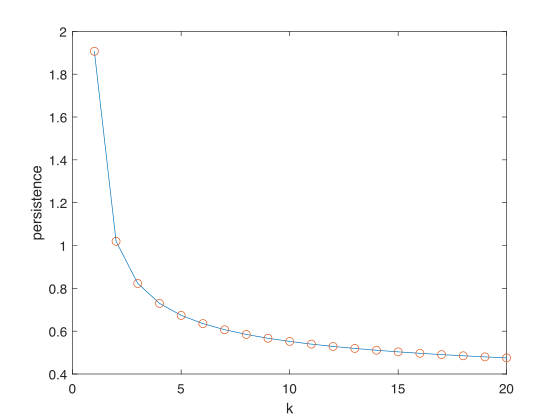
\includegraphics[width=.4\textwidth]{c2_figures/Persistence.png}
\caption{Plot of $0.7$-persistence vs. $k$ for a point $x$ that is distance 1 from all sheets of the conic domain $W_k^n$, as in Proposition \ref{prop:orthants}.}\label{FIG:Persistence}
\end{figure}


In our experiments, we numerically estimate $\gamma$-persistence via a bisection algorithm that we term the Bracketing Algorithm (Appendix \ref{sec:bracketing}).  Briefly, the algorithm first chooses search space bounds $\sigma_{\min}$ and $\sigma_{\max}$ such that $x$ is  $(\gamma,\sigma_{\min})$-stable but is not $(\gamma,\sigma_{\max})$-stable with respect to $\CC$, and then proceeds to evaluate stability by bisection until an approximation of $\sigma_\gamma^*$ is obtained.


%This is accomplished by a bracketing procedure: we first expand the search space bounds $\sigma_{\min}$ and $\sigma_{\max}$ so that the average number of samples at these bounds are below (respectively above) $\gamma$.  This search space is then sequentially bisected to identify a $\sigma$ corresponding with $\gamma$ (the full algorithm is presented in the Appendix).

%We can compute approximate the $\gamma$-persistence using a bisection algorithm we call the Bracketing Algorithm. The Bracketing Algorithm is given as Algorithm \ref{bracketing} in Appendix \ref{sec:bracketing}.  

%\renewcommand{\baselinestretch}{1.0}

%\renewcommand{\baselinestretch}{1.5}

\section{Experiments} \label{sec:experiments}

%???Did we try Carlini-Wagner method? -- B2 not yet, working on it for Imnet

% B2 -- here's what we have ready to go

In this section we investigate the stability and persistence behavior of natural and adversarial examples for MNIST ~\cite{MNIST} and ImageNet ~\cite{ILSVRC15} using a variety of different classifiers. For each set of image samples generated for a particular dataset, model, and attack protocol, we study $(\gamma,\sigma)$-stability and $\gamma$-persistence of both natural and adversarial images, and also compute persistence along trajectories from natural to adversarial images. In general, we use $\gamma = 0.7$, and note that the observed behavior does not change significantly for small changes in $\gamma$. While most of the adversarial attacks considered here have a clear target class, the measurement of persistence does not require considering a particular candidate class. These experiments were performed using PyTorch on an HPC configured with 28 CPUs, 192gb of memory, and 1 nvidia p100 GPU per node. Total compute time needed to generate the results presented was approximately 300 Teraflop/s-days. 




% Adversarial examples are generated using Iterative Gradient Sign Method (IGSM) ~\cite{kurakin_adversarial_2016}, which is an iterative version of the Fast Gradient Sign Method (FGSM) \cite{goodfellow_explaining_2014}, as well as the more primitive Limited-memory Broyden-Fletcher-Goldfarb-Shanno (L-BFGS) optimization algorithm ~\cite{liu1989limited}. 

% The neighborhoods around datapoints and adversarial examples are sampled using Gaussians with varying standard deviation $\sigma$, and Algorithm \ref{bracketing} is used to approximate $\gamma$-persistence corresponding to $\gamma=0.7$. The resultant $0.7$-persistence $\sigma_{.7}^*$ statistically identifies examples as being $(0.7,\sigma_{.7}^*)$-stable, meaning that 70\% of the samples drawn from a Gaussian with standard deviation $\sigma$ are classified the same as the original class by the model. 

% The first test of the ideas behind $(\gamma, \sigma)$-stability is to consider what happens to Gaussian samples as the standard deviation is increased from zero. To this end, for each choice of $\sigma$ ??Where?? we took 1000 samples around the original image or adversarial image and plotted the count of how many were classified with each label. These results are seen in Figures ???? %Algorithm \ref{bracketing} is used to approximate $\gamma$-persistence corresponding to $\gamma=0.7$. The resultant $0.7$-persistence $\sigma$ statistically identifies examples as being $(0.7,\sigma)$-stable, meaning that 70\% of the samples drawn from a Gaussian with standard deviation $\sigma$ are classified the same as the original class by the model. 
% In order to understand the impact of model complexity on $(\gamma, \sigma)$-stability of adversarial examples, we considered the framework of ~\cite{Szegedy2013}, looking at a variety of networks of differing complexities, including both fully-connected and convolutional neural networks.


\subsection{MNIST Experiments}

%The MNIST dataset consists of 28 by 28 pixels, so it can naturally be considered as a data set on a 784 dimensional vector space. The size of this data makes it ideal for initial testing. 
Since MNIST is relatively small compared to ImageNet, we trained several classifiers with various architectures and complexities and implemented the adversarial attacks directly. Adversarial examples were generated against each of these models using Iterative Gradient Sign Method (IGSM ~\cite{kurakin_adversarial_2016}) and Limited-memory Broyden-Fletcher-Goldfarb-Shanno (L-BFGS ~\cite{liu1989limited}).


 

\subsubsection{Investigation of $(\gamma, \sigma)$-stability on MNIST}\label{sec:mnist}

We begin with a fully connected ReLU network with layers of size 784, 100, 20, and 10 and small regularization $\lambda = 10^{-7}$ which is trained on the standard MNIST training set. We then start with a randomly selected MNIST test image $x_1$ from the \texttt{1}'s class and generate adversarial examples $x_0,x_2,\dots,x_9$ using IGSM for each target class other than \texttt{1}. The neighborhoods around each $x_i$ are examined by generating 1000 i.i.d. samples from $N(x_i,\sigma^2I)$ for each of 100 equally spaced standard deviations $\sigma\in(0,1.6)$. Figure \ref{fgsmo} shows the results of the Gaussian perturbations of a natural example $x_1$ of the class labeled \texttt{1} and the results of Gaussian perturbations of the adversarial example $x_0$ targeted at the class labeled \texttt{0}. We provide other examples of $x_2,\ldots,x_9$ in the supplementary materials. Note that the original image is very stable under perturbation, while the adversarial image is not. 

% \begin{figure}[ht]
% \includegraphics[trim=200 80 100 100, clip, width = .9\textwidth]
% %[trim=200 80 100 100, clip,width=15cm]
% {c2_figures/Image918-O1Anone_varx40.png}
% \caption{Frequency of each class in Gaussian samples with increasing variance around an adversarial image of a $1$ targeted at $0$ generated using IGSM. The adversarial class is shown as a red curve. The natural image class is shown in black. The bottom shows example sample images.}
% \label{fgsmo}
% \end{figure}


% \begin{figure}[ht]
% \includegraphics[trim=200 80 100 100,clip, width = .9\textwidth]
% %[trim=200 80 100 100, clip,width=15cm]
% {c2_figures/Image918-O1A0_varx40.png}
% \caption{Frequency of each class in Gaussian samples with increasing variance around an adversarial image of a $1$ targeted at $0$ generated using IGSM. The adversarial class is shown as a red curve. The natural image class is shown in black. The bottom shows example sample images. }
% \label{fgsma}
% \end{figure}

\begin{figure}[ht]
\includegraphics[width = .49\textwidth]
%[trim=200 80 100 100, clip,width=15cm]
{c2_figures/MNIST1.png} \includegraphics[width = .49\textwidth]
%[trim=200 80 100 100, clip,width=15cm]
{c2_figures/MNIST10.png}
\caption{Frequency of each class in Gaussian samples with increasing variance around a natural image of class \texttt{1} (left) and around an adversarial attack of that image targeted at \texttt{0} generated using IGSM (right). The adversarial class (\texttt{0}) is shown as a red curve. The natural image class (\texttt{1}) is shown in black. Bottoms show example sample images at different standard deviations for natural (left) and adversarial (right) examples.}\label{fgsmo}
\end{figure}



\subsubsection{Persistence of adversarial examples for MNIST}

% For adversarial examples, we are particularly interested in comparing the classification counts around each example relative to the distortion ($\|x\|_2/\sqrt{n}$) introduced to generate the example. We then compute $0.7$-persistence for a variety of models and samples and summarize these results.

To study persistence of adversarial examples on MNIST, we take the same network architecture as in the previous subsection and randomly select 200 MNIST images. For each image, we used IGSM to generate 9 adversarial examples (one for each target class) yielding a total of 1800 adversarial examples. In addition, we randomly sampled 1800 natural MNIST images. For each of the 3600 images, we computed $0.7$-persistence; the results are shown in Figure \ref{fig:IGSMpersistenceMNIST}. One sees that $0.7$-persistence of adversarial examples tends to be significantly smaller than that of natural examples for this classifier, indicating that they are generally less stable than natural images. We will see subsequently that this behavior is typical.

%and generate adversarial examples using IGSM for each of 200 randomly selected MNIST images to each possible target other than the original class (9 total targets) for a total of 1800 adversarial examples. 
 %The images were processed using a bisection algorithm (Algorithm \ref{bracketing} in the supplementary materials) to compute $0.7$-persistence. The results are aggregated in Figure \ref{fig:IGSMpersistenceMNIST}.
\begin{figure}[h!]
\centering
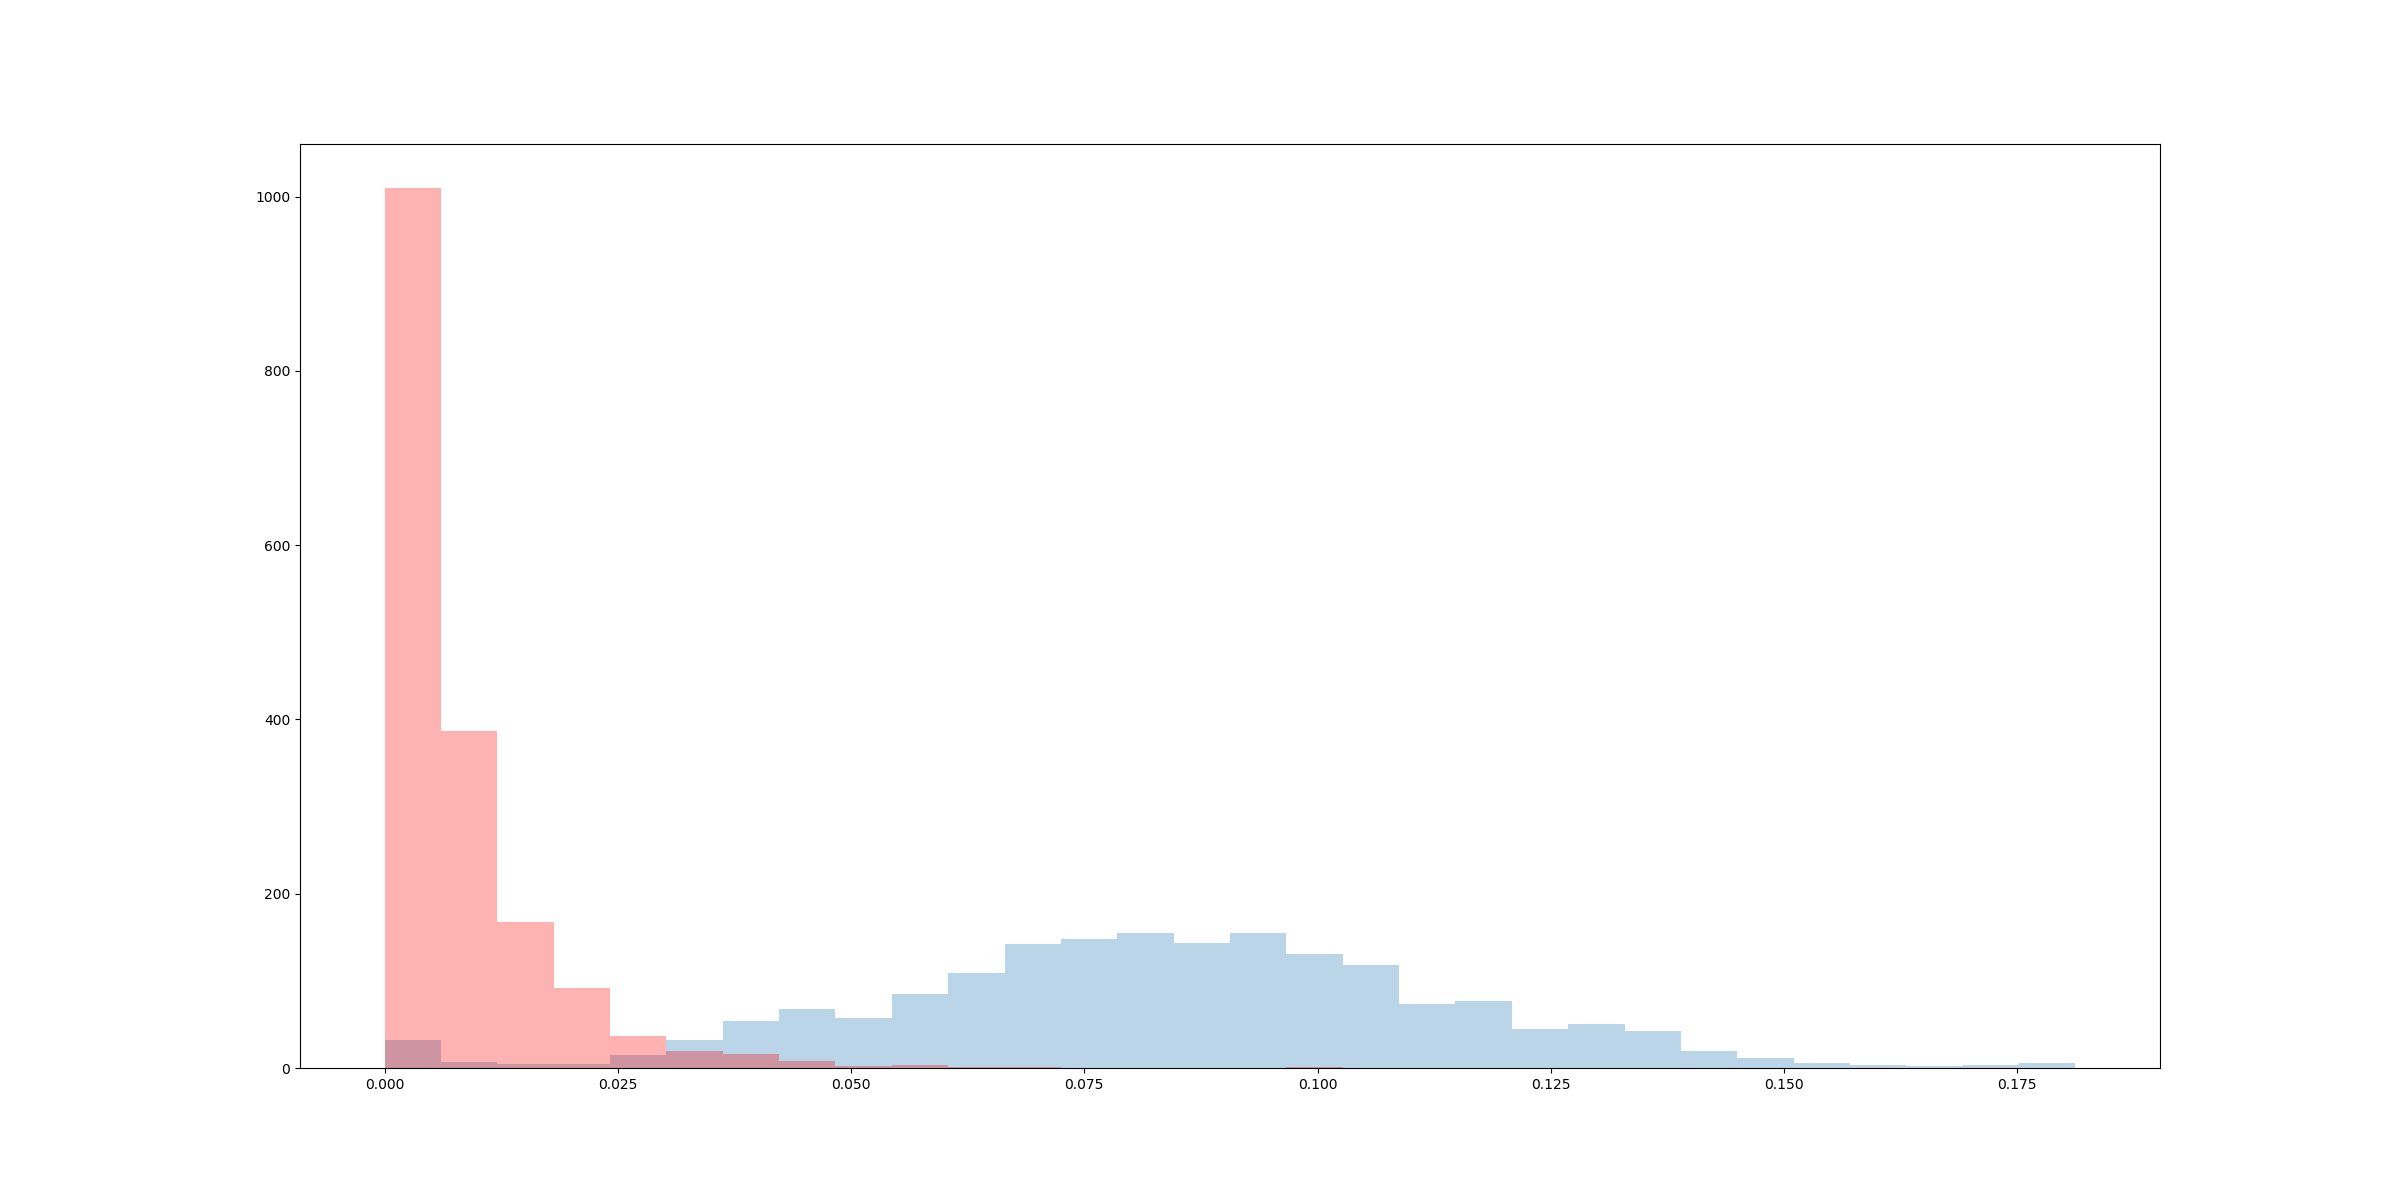
\includegraphics[trim=200 80 100 100, clip,width=.5\textwidth]{c2_figures/original_hist.png}
\caption{Histogram of $0.7$-persistence of IGSM-based adversarial examples (red) and natural examples (blue) on MNIST. %The histogram shows that $0.7$-persistence for adversarial examples tends to be smaller than $0.7$-persistence for natural examples.
}
%\label{fgsmh}
\label{fig:IGSMpersistenceMNIST}
\end{figure}
% TODO : expand figure 13 with a wide sample of adversarial versus natural examples from imagenet. 
%In this experiment, the adversarial examples (red) tended to have a lower $0.7$- persistence than natural images (blue), indicating that they were much less stable than the natural images. %DG: I HAVE REMOVED: We can define a linear classifier on these $\gamma$-persistence values which will identify adversarial attacks with 98\% accuracy. 

%\subsection{Effects of network complexity on persistence}
%{Neighborhood sampling of L-BFGS adversarial examples for MNIST}

Next, we investigate the relationship of network complexity and $(\gamma,\sigma)$-stability by revisiting the now classic work of ~\cite{Szegedy2013} on adversarial examples. 
%In these experiments, we used L-BFGS technique from \cite{Szegedy2013} to prepare adversarial examples. The same network architectures and examples were subjected to $0.7$-persistence analysis to determine the correspondence of stability with network accuracy and average distortion. In this case we will loosely define complexity as the effective number of parameters of a network and distortion is the $\ell^2$ norm divided by square root of the dimension $n$. 
%[??DG??: We need to define complexity and add it to the table]
%\subsubsection{Re-examining Szegedy Results with sampling}
%
Table \ref{table1} recreates and adds on to part of \cite[Table 1]{Szegedy2013} in which networks of differing complexity are trained and attacked using L-BFGS. The table contains new columns showing the average $0.7$-persistence for both natural and adversarial examples for each network, as well as the average distortion for the adversarial examples. The distortion is the $\ell^2$-norm divided by square root of the dimension $n$. The first networks listed are of the form FC10-k, and are fully connected single layer ReLU networks that map each input vector $x \in \RR^{784}$ to an output vector $y \in \RR^{10}$ with a regularization added to the objective function of the form $\lambda\Norm{w}_2/N$, where $\lambda = 10^{-k}$ and $N$ is the number of parameters in the weight vector $w$ defining the network. The higher values of $\lambda$ indicate more regularization.  
%added as regularization to the objective function during training. FC10-2 is the same except with $\lambda = 10^{-2}$ and FC10-0 has $\lambda=1$ (a very large coefficient for regularization). 
FC100-100-10 and FC200-200-10 are networks with 2 hidden layers (with 100 and 200 nodes, respectively) with regularization added for each layer of perceptrons with the $\lambda$ for each layer equal to $10^{-5}, 10^{-5}$, and  $10^{-6}$. Training for these networks was conducted with a fixed number of epochs (typically 21). For the bottom half of Table \ref{table1}, we also considered networks with four convolutional layers plus a max-pooling layer connected by ReLU to a fully connected hidden layer with increasing numbers of channels denoted as as ``C-Ch,'' where C reflects that this is a CNN and Ch denotes the number of channels. A more detailed description of these networks can be found in Appendix \ref{appendix:CNNs}.

\begin{table}[ht]
\centering
\caption{Recreation of ~\cite[Table 1]{Szegedy2013} for the MNIST dataset.  For each network, we show Testing Accuracy (in \%), Average Distortion ($\|x\|_2/\sqrt{n}$) of adversarial examples, and new columns show average $0.7$-persistence values for natural (Nat) and adversarial (Adv) images. 300 natural and 300 adversarial examples generated with L-BFGS were used for each aggregation.}
\label{table1}
\begin{tabular}{lllll}
\toprule
Network & Test Acc & Avg Dist & Persist (Nat) & Persist (Adv) \\
\midrule
FC10-4 & 92.09 & 0.123 & 0.93 & 1.68\\
FC10-2 & 90.77 & 0.178 & 1.37 & 4.25\\
FC10-0 & 86.89 & 0.278 & 1.92 & 12.22\\
FC100-100-10 & 97.31 & 0.086 & 0.65 & 0.56 \\
FC200-200-10 & 97.61 & 0.087 & 0.73 & 0.56 \\
\midrule
C-2 & 95.94 & 0.09 & 3.33 & 0.027 \\
C-4 & 97.36 & 0.12 & 0.35 & 0.027 \\
C-8 & 98.50 & 0.11 & 0.43  & 0.0517 \\
C-16 & 98.90 & 0.11 & 0.53 & 0.0994 \\
C-32 & 98.96 & 0.11 & 0.78 & 0.0836 \\
C-64 & 99.00 & 0.10 & 0.81 & 0.0865 \\
C-128 & 99.17 & 0.11 & 0.77 & 0.0883 \\
C-256 & 99.09 & 0.11  & 0.83 & 0.0900 \\
C-512 & 99.22 & 0.10 & 0.793 & 0.0929 \\
%C-128-2000 & 99.07 & 0.11 & 89.27 & 0.731 & 0.136 \\
%C-128-4000 & 99.13 & 0.098 & 89.71 & 1.024 & 0.424 \\
%C-128-4500 & 99.32 & 0.096 & 90.59 & NA & 0.103 \\
%C-128-4700 & 97.48 & 0.079 & 87.16 & NA & NA \\
%C-128-4708 & 95.69 & 0.077 & 80.90 & 0.15 & 0.0307 \\
%C-128-4712 & 93.04 & 0.135 & 57.11 & 0.14 & 0.0296 \\
%C-128-4714 & 78.87 & 0.211 & 41.61 & 0.059 & 0.012 \\
%C-128-4715 & 65.99 & 0.831 & 23.61 & NA & 0.0092 \\ \hline
\bottomrule
\end{tabular}
\end{table}

The main observation from Table \ref{table1} is that for higher complexity networks,
adversarial examples tend to have smaller persistence than natural examples. Histograms reflecting these observations can be found in the supplemental material. %This can be seen as well in Figure \ref{fig:FC200-200-10}, which shows the $0.7$-persistence for natural and adversarial examples for the network FC200-200-10. 
Another notable takeaway is that for models with fewer effective parameters, the attack distortion necessary to generate a successful attack is so great that the resulting image is often more stable than a natural image under that model, as seen particularly in the FC10 networks. Once there are sufficiently many parameters available in the neural network, we found that both the average distortion of the adversarial examples and the average $0.7$-persistence of the adversarial examples tended to be smaller. This observation is consistent with the idea that networks with more parameters are more likely to exhibit decision boundaries with more curvature.

% \begin{figure}[h!]
% \centering
% 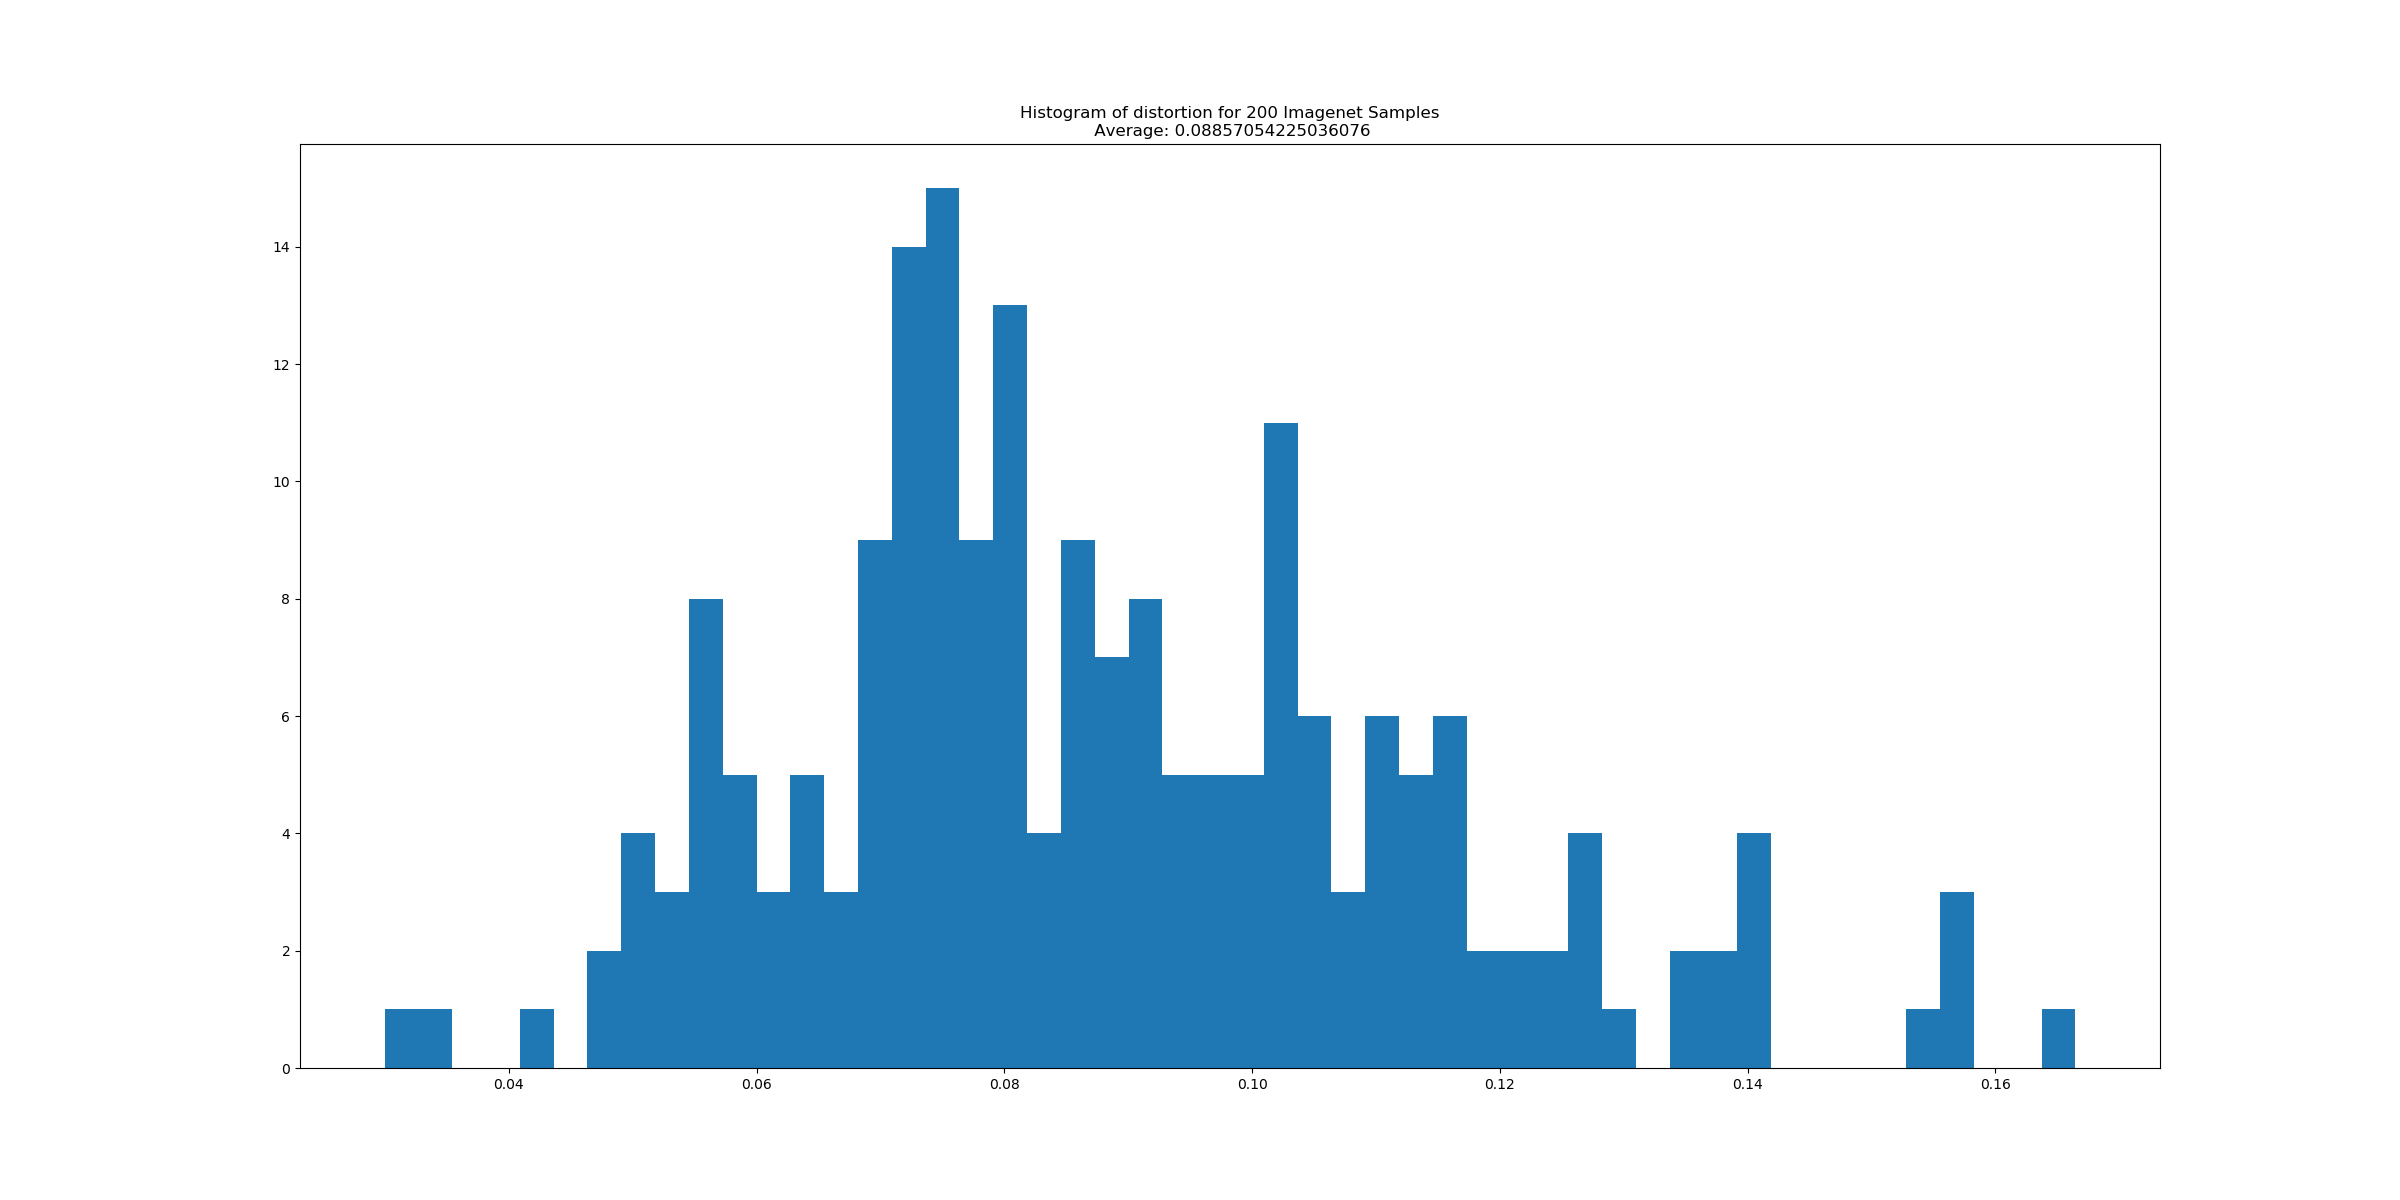
\includegraphics[trim=200 80 100 100, clip,width=7cm]{c2_figures/FC200-200-10-distortion_hist.png}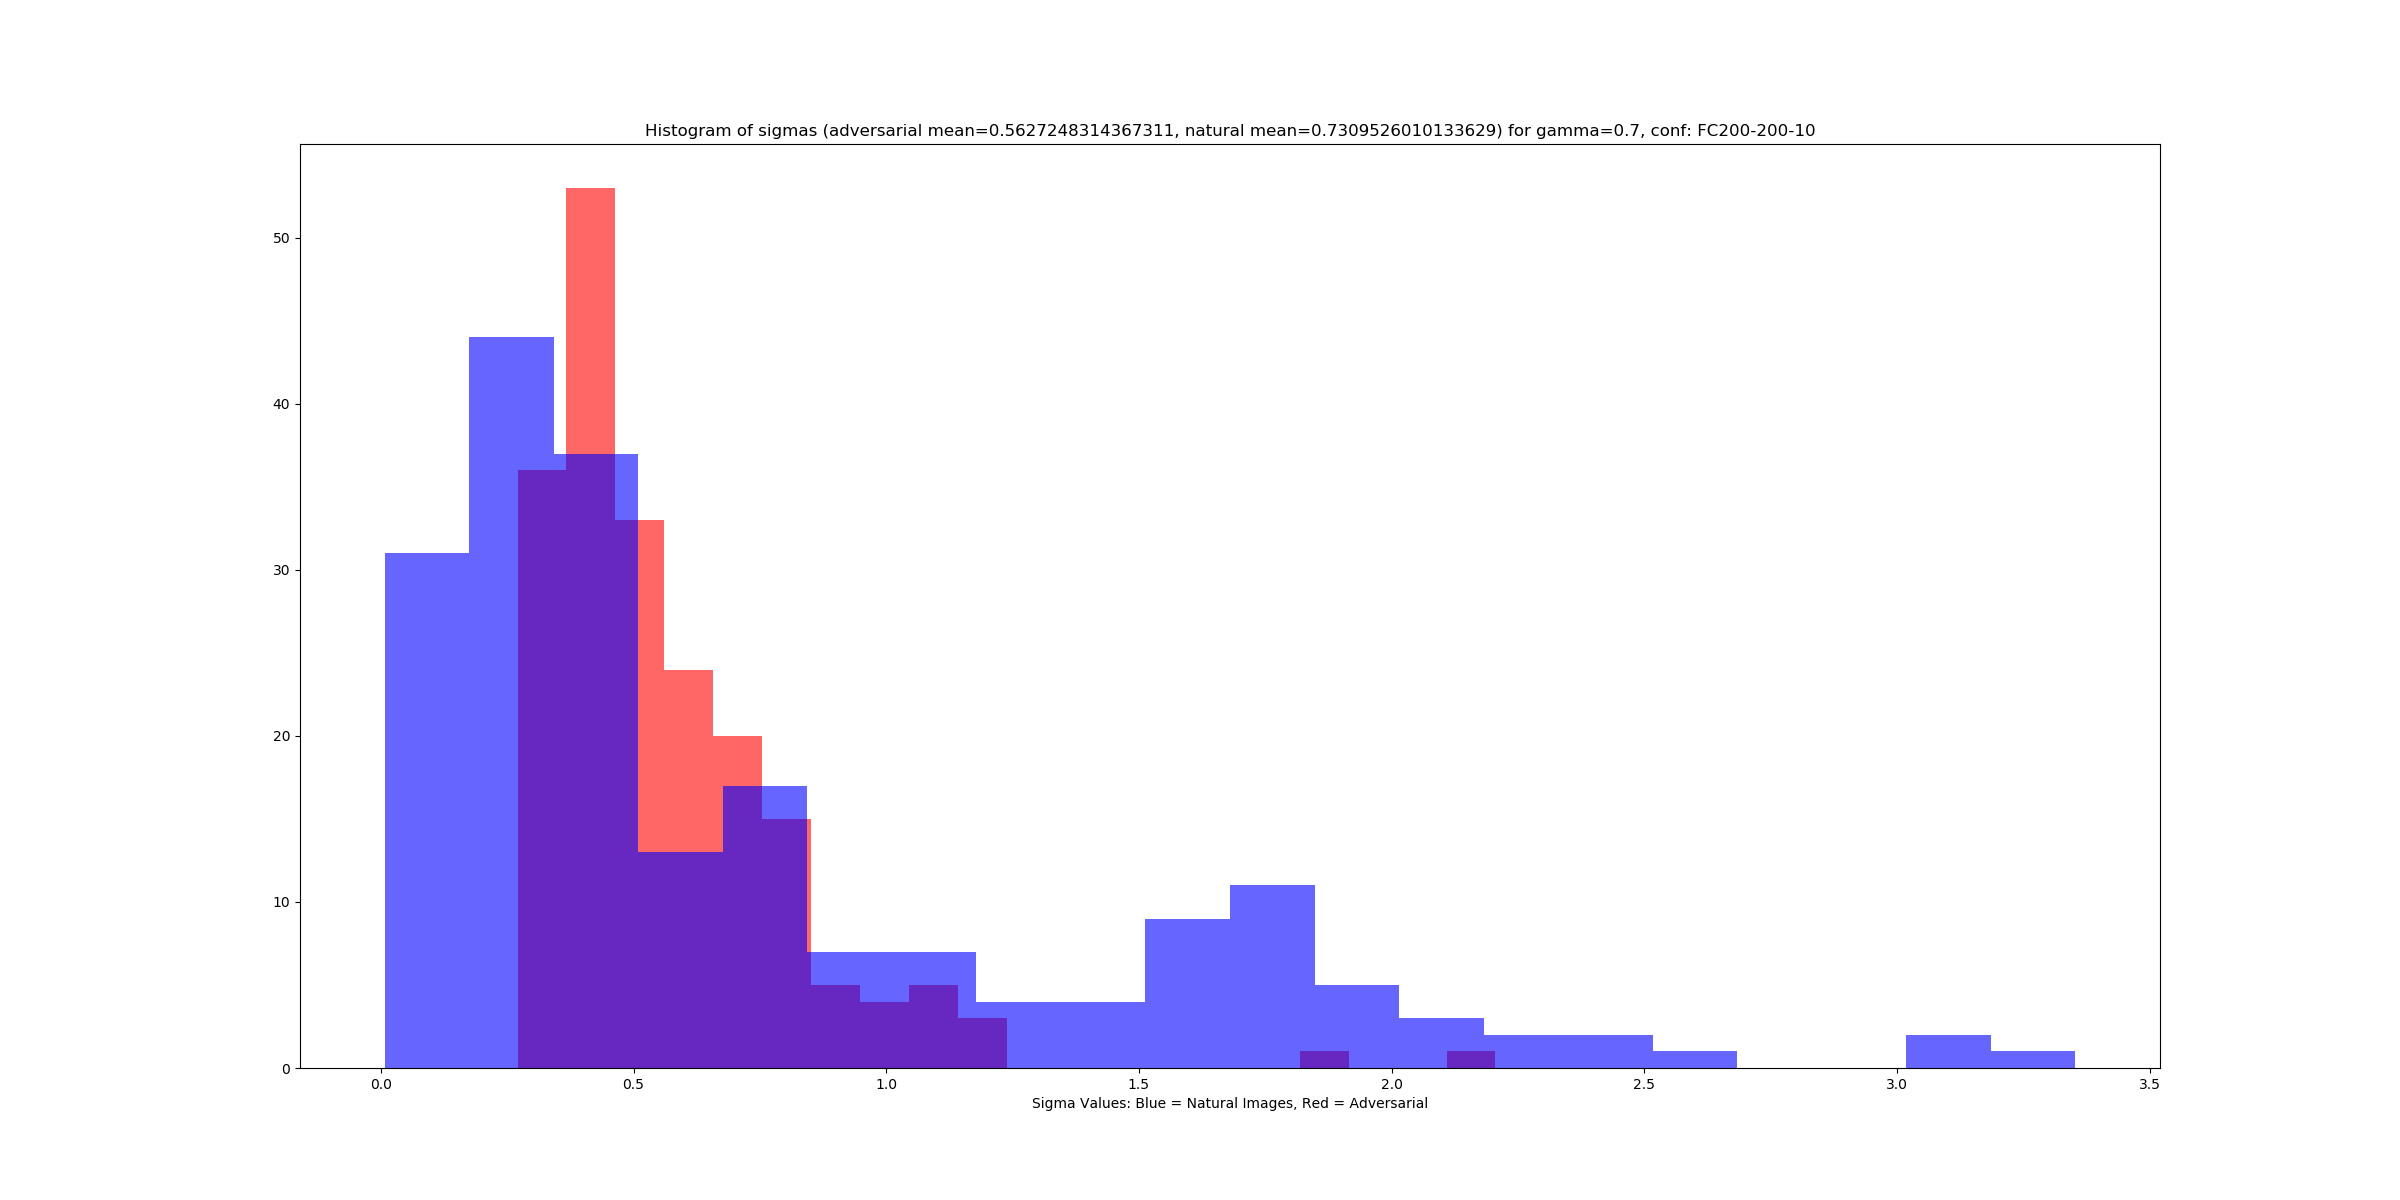
\includegraphics[trim=200 80 100 100, clip,width=7cm]{c2_figures/FC200-200-10-gamma1_hist.png}

% \caption{Average distortion for adversarial examples (left) and $0.7$-persistence (right) for FC200-200-10 in Table \ref{table1}}
% \label{fig:FC200-200-10}
% \end{figure}

%B^2 -- we're not using state of the art classifiers... used pre-trained classifiers in order to capture state-of-the-art methods. In particular, we

\subsection{Results on ImageNet}

% For ImageNet, various pretrained networks (vgg16, alexnet, resnet18, densenet161, and squeezenet) were downloaded using torchvision and were attacked with a variety of attack methods %(PGD, FGSM, APGD, CW, ??) 
% using the torchattacks package \cite{kim2021torchattacks}. In all of our tests, we begin with a subset of validation images from the given dataset and generate a collection of adversarial attacks based on those images for each combination of model and attack protocol. 

For ImageNet ~\cite{Imagenet-old}, we used pre-trained ImageNet classification models, including alexnet \cite{alexnet} and vgg16 \cite{simonyan2014very}.
%, resnet18, squeezenet, and densenet161 \cite{}
We then generated attacks based on the ILSVRC 2015 ~\cite{ILSVRC15} validation images for each of these networks using a variety of modern attack protocols, including Fast Gradient Sign Method (FGSM ~\cite{goodfellow_explaining_2014}), Momentum Iterative FGSM (MIFGSM ~\cite{dongMIFGSM}), Basic Iterative Method (BIM ~\cite{kurakin_adversarial_2016}), Projected Gradient Descent (PGD ~\cite{madry_towards_2017}), Randomized FGSM (R+FGSM ~\cite{tramer2018ensemble}), and Carlini-Wagner (CW ~\cite{carlini_towards_2016}). These were all generated using the TorchAttacks \cite{kim2021torchattacks} toolset.
%We first directly examine neighborhood classification counts as with MNIST and observe a similar dichotomy between original and attacked images. 

\subsubsection{Investigation of $(\gamma, \sigma)$-stability on ImageNet}

In this section, we show the results of Gaussian neighborhood sampling in ImageNet. Figures \ref{fig:imagenet_adv} and \ref{fig:persistent_interpimage} arise from vgg16 and adversarial examples created with BIM; results for other networks and attack strategies are similar, with additional figures in the supplementary material. Figure \ref{fig:imagenet_adv} (left) begins with an image $x$ with label \texttt{goldfinch}. For each equally spaced $\sigma\in(0,2)$, 100 i.i.d. samples were drawn from the Gaussian distribution $N(x,\sigma^2I)$, and the counts of the vgg16 classification for each label are shown. In Figure \ref{fig:imagenet_adv} (right), we see the same plot, but for an adversarial example targeted at the class \texttt{indigo\_bunting}, which is another type of bird, using the BIM attack protocol. %There are similar results with other attack protocols, as described in the supplementary materials.

The key observation in Figure \ref{fig:imagenet_adv} is that the frequency of the class of the adversarial example (\texttt{indigo\_bunting}, shown in red) falls off much quicker than the class for the natural example (\texttt{goldfinch}, shown in black). In this particular example, the original class appears again after the adversarial class becomes less prevalent, but only for a short period of $\sigma$, after which other classes begin to dominate. In some examples the original class does not dominate at all after the decline of the adversarial class. The adversarial class almost never dominates for a long period of $\sigma$. 


% \begin{figure}[ht]
% \centering
% \includegraphics[width = .9\textwidth]
% %[trim=200 80 100 100, clip,width=15cm]
% {./c2_figures/ILSVRC2012_val_00001274-vgg16-sampling.png}
% %\caption{Frequency of each class in Gaussian samples with increasing variance around an adversarial image of a $1$ targeted at $0$ generated using IGSM. The adversarial class is shown as a red curve. The natural image class is shown in black. The bottom shows example sample images.}
% \label{fig:imagenet_natural}
% \caption{Frequency of each class in Gaussian samples with increasing variance around a goldfinch image. Bottom shows example sample images. }
% \end{figure}
%
% \begin{figure}[p]
% \centering
% \includegraphics[width = .9\textwidth]
% {./c2_figures/IMNET-class-11-vgg16-RFGSM-48-attack_data-023.png}
% \end{figure}

\begin{figure}[ht]
\centering
\includegraphics[width = .49\textwidth]
%[trim=200 80 100 100, clip,width=15cm]
{./c2_figures/ILSVRC2012_val_00001274-vgg16-sampling.png}
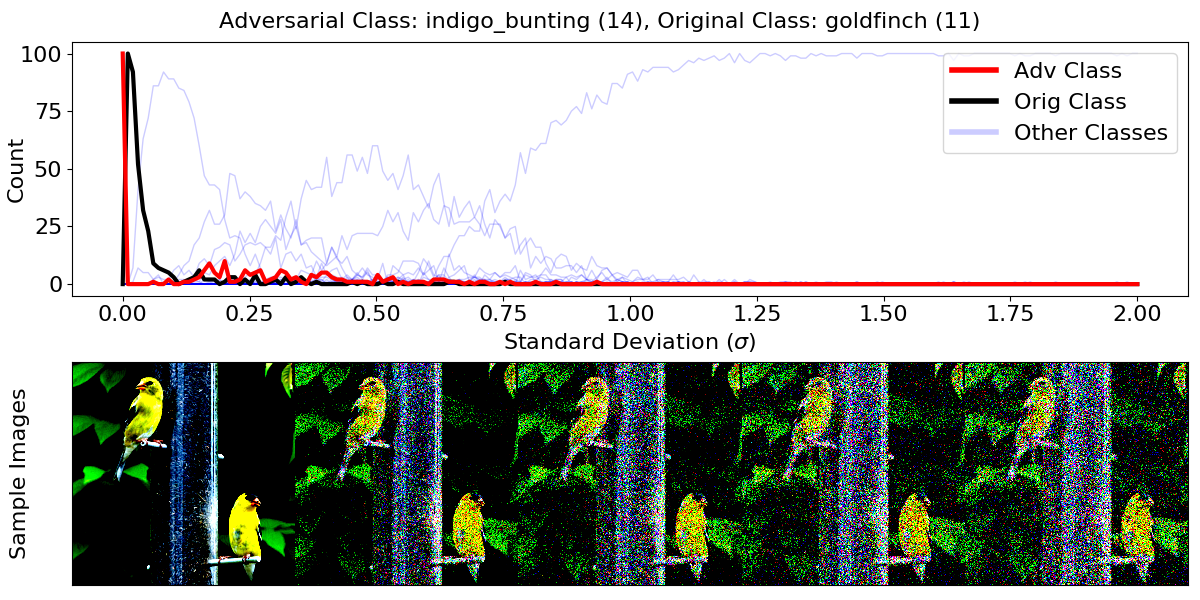
\includegraphics[width = .49\textwidth]
{./c2_figures/IMNET-class-11-vgg16-BIM-48-attack_data-023.png}
%%% Creator: Matplotlib, PGF backend
%%
%% To include the figure in your LaTeX document, write
%%   \input{<filename>.pgf}
%%
%% Make sure the required packages are loaded in your preamble
%%   \usepackage{pgf}
%%
%% and, on pdftex
%%   \usepackage[utf8]{inputenc}\DeclareUnicodeCharacter{2212}{-}
%%
%% or, on luatex and xetex
%%   \usepackage{unicode-math}
%%
%% Figures using additional raster images can only be included by \input if
%% they are in the same directory as the main LaTeX file. For loading figures
%% from other directories you can use the `import` package
%%   \usepackage{import}
%%
%% and then include the figures with
%%   \import{<path to file>}{<filename>.pgf}
%%
%% Matplotlib used the following preamble
%%   \usepackage{fontspec}
%%   \setmainfont{DejaVuSerif.ttf}[Path=C:/Users/glickenstein/anaconda3/lib/site-packages/matplotlib/mpl-data/fonts/ttf/]
%%   \setsansfont{DejaVuSans.ttf}[Path=C:/Users/glickenstein/anaconda3/lib/site-packages/matplotlib/mpl-data/fonts/ttf/]
%%   \setmonofont{DejaVuSansMono.ttf}[Path=C:/Users/glickenstein/anaconda3/lib/site-packages/matplotlib/mpl-data/fonts/ttf/]
%%
\begingroup%
\makeatletter%
\begin{pgfpicture}%
\pgfpathrectangle{\pgfpointorigin}{\pgfqpoint{5.000000in}{2.500000in}}%
\pgfusepath{use as bounding box, clip}%
\begin{pgfscope}%
\pgfsetbuttcap%
\pgfsetmiterjoin%
\definecolor{currentfill}{rgb}{1.000000,1.000000,1.000000}%
\pgfsetfillcolor{currentfill}%
\pgfsetlinewidth{0.000000pt}%
\definecolor{currentstroke}{rgb}{1.000000,1.000000,1.000000}%
\pgfsetstrokecolor{currentstroke}%
\pgfsetdash{}{0pt}%
\pgfpathmoveto{\pgfqpoint{0.000000in}{0.000000in}}%
\pgfpathlineto{\pgfqpoint{5.000000in}{0.000000in}}%
\pgfpathlineto{\pgfqpoint{5.000000in}{2.500000in}}%
\pgfpathlineto{\pgfqpoint{0.000000in}{2.500000in}}%
\pgfpathclose%
\pgfusepath{fill}%
\end{pgfscope}%
\begin{pgfscope}%
\pgfsetbuttcap%
\pgfsetmiterjoin%
\definecolor{currentfill}{rgb}{1.000000,1.000000,1.000000}%
\pgfsetfillcolor{currentfill}%
\pgfsetlinewidth{0.000000pt}%
\definecolor{currentstroke}{rgb}{0.000000,0.000000,0.000000}%
\pgfsetstrokecolor{currentstroke}%
\pgfsetstrokeopacity{0.000000}%
\pgfsetdash{}{0pt}%
\pgfpathmoveto{\pgfqpoint{0.300000in}{1.350000in}}%
\pgfpathlineto{\pgfqpoint{4.950000in}{1.350000in}}%
\pgfpathlineto{\pgfqpoint{4.950000in}{2.475000in}}%
\pgfpathlineto{\pgfqpoint{0.300000in}{2.475000in}}%
\pgfpathclose%
\pgfusepath{fill}%
\end{pgfscope}%
\begin{pgfscope}%
\pgfsetbuttcap%
\pgfsetroundjoin%
\definecolor{currentfill}{rgb}{0.000000,0.000000,0.000000}%
\pgfsetfillcolor{currentfill}%
\pgfsetlinewidth{0.803000pt}%
\definecolor{currentstroke}{rgb}{0.000000,0.000000,0.000000}%
\pgfsetstrokecolor{currentstroke}%
\pgfsetdash{}{0pt}%
\pgfsys@defobject{currentmarker}{\pgfqpoint{0.000000in}{-0.048611in}}{\pgfqpoint{0.000000in}{0.000000in}}{%
\pgfpathmoveto{\pgfqpoint{0.000000in}{0.000000in}}%
\pgfpathlineto{\pgfqpoint{0.000000in}{-0.048611in}}%
\pgfusepath{stroke,fill}%
}%
\begin{pgfscope}%
\pgfsys@transformshift{0.511364in}{1.350000in}%
\pgfsys@useobject{currentmarker}{}%
\end{pgfscope}%
\end{pgfscope}%
\begin{pgfscope}%
\definecolor{textcolor}{rgb}{0.000000,0.000000,0.000000}%
\pgfsetstrokecolor{textcolor}%
\pgfsetfillcolor{textcolor}%
\pgftext[x=0.511364in,y=1.252778in,,top]{\color{textcolor}\sffamily\fontsize{16.000000}{19.200000}\selectfont 0.0}%
\end{pgfscope}%
\begin{pgfscope}%
\pgfsetbuttcap%
\pgfsetroundjoin%
\definecolor{currentfill}{rgb}{0.000000,0.000000,0.000000}%
\pgfsetfillcolor{currentfill}%
\pgfsetlinewidth{0.803000pt}%
\definecolor{currentstroke}{rgb}{0.000000,0.000000,0.000000}%
\pgfsetstrokecolor{currentstroke}%
\pgfsetdash{}{0pt}%
\pgfsys@defobject{currentmarker}{\pgfqpoint{0.000000in}{-0.048611in}}{\pgfqpoint{0.000000in}{0.000000in}}{%
\pgfpathmoveto{\pgfqpoint{0.000000in}{0.000000in}}%
\pgfpathlineto{\pgfqpoint{0.000000in}{-0.048611in}}%
\pgfusepath{stroke,fill}%
}%
\begin{pgfscope}%
\pgfsys@transformshift{1.356818in}{1.350000in}%
\pgfsys@useobject{currentmarker}{}%
\end{pgfscope}%
\end{pgfscope}%
\begin{pgfscope}%
\definecolor{textcolor}{rgb}{0.000000,0.000000,0.000000}%
\pgfsetstrokecolor{textcolor}%
\pgfsetfillcolor{textcolor}%
\pgftext[x=1.356818in,y=1.252778in,,top]{\color{textcolor}\sffamily\fontsize{16.000000}{19.200000}\selectfont 0.2}%
\end{pgfscope}%
\begin{pgfscope}%
\pgfsetbuttcap%
\pgfsetroundjoin%
\definecolor{currentfill}{rgb}{0.000000,0.000000,0.000000}%
\pgfsetfillcolor{currentfill}%
\pgfsetlinewidth{0.803000pt}%
\definecolor{currentstroke}{rgb}{0.000000,0.000000,0.000000}%
\pgfsetstrokecolor{currentstroke}%
\pgfsetdash{}{0pt}%
\pgfsys@defobject{currentmarker}{\pgfqpoint{0.000000in}{-0.048611in}}{\pgfqpoint{0.000000in}{0.000000in}}{%
\pgfpathmoveto{\pgfqpoint{0.000000in}{0.000000in}}%
\pgfpathlineto{\pgfqpoint{0.000000in}{-0.048611in}}%
\pgfusepath{stroke,fill}%
}%
\begin{pgfscope}%
\pgfsys@transformshift{2.202273in}{1.350000in}%
\pgfsys@useobject{currentmarker}{}%
\end{pgfscope}%
\end{pgfscope}%
\begin{pgfscope}%
\definecolor{textcolor}{rgb}{0.000000,0.000000,0.000000}%
\pgfsetstrokecolor{textcolor}%
\pgfsetfillcolor{textcolor}%
\pgftext[x=2.202273in,y=1.252778in,,top]{\color{textcolor}\sffamily\fontsize{16.000000}{19.200000}\selectfont 0.4}%
\end{pgfscope}%
\begin{pgfscope}%
\pgfsetbuttcap%
\pgfsetroundjoin%
\definecolor{currentfill}{rgb}{0.000000,0.000000,0.000000}%
\pgfsetfillcolor{currentfill}%
\pgfsetlinewidth{0.803000pt}%
\definecolor{currentstroke}{rgb}{0.000000,0.000000,0.000000}%
\pgfsetstrokecolor{currentstroke}%
\pgfsetdash{}{0pt}%
\pgfsys@defobject{currentmarker}{\pgfqpoint{0.000000in}{-0.048611in}}{\pgfqpoint{0.000000in}{0.000000in}}{%
\pgfpathmoveto{\pgfqpoint{0.000000in}{0.000000in}}%
\pgfpathlineto{\pgfqpoint{0.000000in}{-0.048611in}}%
\pgfusepath{stroke,fill}%
}%
\begin{pgfscope}%
\pgfsys@transformshift{3.047727in}{1.350000in}%
\pgfsys@useobject{currentmarker}{}%
\end{pgfscope}%
\end{pgfscope}%
\begin{pgfscope}%
\definecolor{textcolor}{rgb}{0.000000,0.000000,0.000000}%
\pgfsetstrokecolor{textcolor}%
\pgfsetfillcolor{textcolor}%
\pgftext[x=3.047727in,y=1.252778in,,top]{\color{textcolor}\sffamily\fontsize{16.000000}{19.200000}\selectfont 0.6}%
\end{pgfscope}%
\begin{pgfscope}%
\pgfsetbuttcap%
\pgfsetroundjoin%
\definecolor{currentfill}{rgb}{0.000000,0.000000,0.000000}%
\pgfsetfillcolor{currentfill}%
\pgfsetlinewidth{0.803000pt}%
\definecolor{currentstroke}{rgb}{0.000000,0.000000,0.000000}%
\pgfsetstrokecolor{currentstroke}%
\pgfsetdash{}{0pt}%
\pgfsys@defobject{currentmarker}{\pgfqpoint{0.000000in}{-0.048611in}}{\pgfqpoint{0.000000in}{0.000000in}}{%
\pgfpathmoveto{\pgfqpoint{0.000000in}{0.000000in}}%
\pgfpathlineto{\pgfqpoint{0.000000in}{-0.048611in}}%
\pgfusepath{stroke,fill}%
}%
\begin{pgfscope}%
\pgfsys@transformshift{3.893182in}{1.350000in}%
\pgfsys@useobject{currentmarker}{}%
\end{pgfscope}%
\end{pgfscope}%
\begin{pgfscope}%
\definecolor{textcolor}{rgb}{0.000000,0.000000,0.000000}%
\pgfsetstrokecolor{textcolor}%
\pgfsetfillcolor{textcolor}%
\pgftext[x=3.893182in,y=1.252778in,,top]{\color{textcolor}\sffamily\fontsize{16.000000}{19.200000}\selectfont 0.8}%
\end{pgfscope}%
\begin{pgfscope}%
\pgfsetbuttcap%
\pgfsetroundjoin%
\definecolor{currentfill}{rgb}{0.000000,0.000000,0.000000}%
\pgfsetfillcolor{currentfill}%
\pgfsetlinewidth{0.803000pt}%
\definecolor{currentstroke}{rgb}{0.000000,0.000000,0.000000}%
\pgfsetstrokecolor{currentstroke}%
\pgfsetdash{}{0pt}%
\pgfsys@defobject{currentmarker}{\pgfqpoint{0.000000in}{-0.048611in}}{\pgfqpoint{0.000000in}{0.000000in}}{%
\pgfpathmoveto{\pgfqpoint{0.000000in}{0.000000in}}%
\pgfpathlineto{\pgfqpoint{0.000000in}{-0.048611in}}%
\pgfusepath{stroke,fill}%
}%
\begin{pgfscope}%
\pgfsys@transformshift{4.738636in}{1.350000in}%
\pgfsys@useobject{currentmarker}{}%
\end{pgfscope}%
\end{pgfscope}%
\begin{pgfscope}%
\definecolor{textcolor}{rgb}{0.000000,0.000000,0.000000}%
\pgfsetstrokecolor{textcolor}%
\pgfsetfillcolor{textcolor}%
\pgftext[x=4.738636in,y=1.252778in,,top]{\color{textcolor}\sffamily\fontsize{16.000000}{19.200000}\selectfont 1.0}%
\end{pgfscope}%
\begin{pgfscope}%
\definecolor{textcolor}{rgb}{0.000000,0.000000,0.000000}%
\pgfsetstrokecolor{textcolor}%
\pgfsetfillcolor{textcolor}%
\pgftext[x=2.625000in,y=0.982162in,,top]{\color{textcolor}\sffamily\fontsize{16.000000}{19.200000}\selectfont Standard Deviation (\(\displaystyle \sigma\))}%
\end{pgfscope}%
\begin{pgfscope}%
\pgfsetbuttcap%
\pgfsetroundjoin%
\definecolor{currentfill}{rgb}{0.000000,0.000000,0.000000}%
\pgfsetfillcolor{currentfill}%
\pgfsetlinewidth{0.803000pt}%
\definecolor{currentstroke}{rgb}{0.000000,0.000000,0.000000}%
\pgfsetstrokecolor{currentstroke}%
\pgfsetdash{}{0pt}%
\pgfsys@defobject{currentmarker}{\pgfqpoint{-0.048611in}{0.000000in}}{\pgfqpoint{0.000000in}{0.000000in}}{%
\pgfpathmoveto{\pgfqpoint{0.000000in}{0.000000in}}%
\pgfpathlineto{\pgfqpoint{-0.048611in}{0.000000in}}%
\pgfusepath{stroke,fill}%
}%
\begin{pgfscope}%
\pgfsys@transformshift{0.300000in}{1.401136in}%
\pgfsys@useobject{currentmarker}{}%
\end{pgfscope}%
\end{pgfscope}%
\begin{pgfscope}%
\definecolor{textcolor}{rgb}{0.000000,0.000000,0.000000}%
\pgfsetstrokecolor{textcolor}%
\pgfsetfillcolor{textcolor}%
\pgftext[x=0.061393in, y=1.316718in, left, base]{\color{textcolor}\sffamily\fontsize{16.000000}{19.200000}\selectfont 0}%
\end{pgfscope}%
\begin{pgfscope}%
\pgfsetbuttcap%
\pgfsetroundjoin%
\definecolor{currentfill}{rgb}{0.000000,0.000000,0.000000}%
\pgfsetfillcolor{currentfill}%
\pgfsetlinewidth{0.803000pt}%
\definecolor{currentstroke}{rgb}{0.000000,0.000000,0.000000}%
\pgfsetstrokecolor{currentstroke}%
\pgfsetdash{}{0pt}%
\pgfsys@defobject{currentmarker}{\pgfqpoint{-0.048611in}{0.000000in}}{\pgfqpoint{0.000000in}{0.000000in}}{%
\pgfpathmoveto{\pgfqpoint{0.000000in}{0.000000in}}%
\pgfpathlineto{\pgfqpoint{-0.048611in}{0.000000in}}%
\pgfusepath{stroke,fill}%
}%
\begin{pgfscope}%
\pgfsys@transformshift{0.300000in}{2.423864in}%
\pgfsys@useobject{currentmarker}{}%
\end{pgfscope}%
\end{pgfscope}%
\begin{pgfscope}%
\definecolor{textcolor}{rgb}{0.000000,0.000000,0.000000}%
\pgfsetstrokecolor{textcolor}%
\pgfsetfillcolor{textcolor}%
\pgftext[x=-0.221376in, y=2.339445in, left, base]{\color{textcolor}\sffamily\fontsize{16.000000}{19.200000}\selectfont 100}%
\end{pgfscope}%
\begin{pgfscope}%
\definecolor{textcolor}{rgb}{0.000000,0.000000,0.000000}%
\pgfsetstrokecolor{textcolor}%
\pgfsetfillcolor{textcolor}%
\pgftext[x=-0.151931in,y=1.912500in,,bottom,rotate=90.000000]{\color{textcolor}\sffamily\fontsize{16.000000}{19.200000}\selectfont Count}%
\end{pgfscope}%
\begin{pgfscope}%
\pgfpathrectangle{\pgfqpoint{0.300000in}{1.350000in}}{\pgfqpoint{4.650000in}{1.125000in}}%
\pgfusepath{clip}%
\pgfsetrectcap%
\pgfsetroundjoin%
\pgfsetlinewidth{1.003750pt}%
\definecolor{currentstroke}{rgb}{0.000000,0.000000,1.000000}%
\pgfsetstrokecolor{currentstroke}%
\pgfsetstrokeopacity{0.200000}%
\pgfsetdash{}{0pt}%
\pgfpathmoveto{\pgfqpoint{0.511364in}{1.401136in}}%
\pgfpathlineto{\pgfqpoint{2.848047in}{1.401136in}}%
\pgfpathlineto{\pgfqpoint{2.869290in}{1.411364in}}%
\pgfpathlineto{\pgfqpoint{2.890532in}{1.401136in}}%
\pgfpathlineto{\pgfqpoint{2.954260in}{1.401136in}}%
\pgfpathlineto{\pgfqpoint{2.996745in}{1.421591in}}%
\pgfpathlineto{\pgfqpoint{3.017988in}{1.401136in}}%
\pgfpathlineto{\pgfqpoint{3.039230in}{1.401136in}}%
\pgfpathlineto{\pgfqpoint{3.060473in}{1.411364in}}%
\pgfpathlineto{\pgfqpoint{3.081715in}{1.401136in}}%
\pgfpathlineto{\pgfqpoint{3.102958in}{1.401136in}}%
\pgfpathlineto{\pgfqpoint{3.124201in}{1.411364in}}%
\pgfpathlineto{\pgfqpoint{3.145443in}{1.401136in}}%
\pgfpathlineto{\pgfqpoint{3.357869in}{1.401136in}}%
\pgfpathlineto{\pgfqpoint{3.379111in}{1.421591in}}%
\pgfpathlineto{\pgfqpoint{3.400354in}{1.401136in}}%
\pgfpathlineto{\pgfqpoint{3.506567in}{1.401136in}}%
\pgfpathlineto{\pgfqpoint{3.527810in}{1.411364in}}%
\pgfpathlineto{\pgfqpoint{3.549052in}{1.401136in}}%
\pgfpathlineto{\pgfqpoint{3.634022in}{1.401136in}}%
\pgfpathlineto{\pgfqpoint{3.655265in}{1.411364in}}%
\pgfpathlineto{\pgfqpoint{3.676508in}{1.401136in}}%
\pgfpathlineto{\pgfqpoint{3.697750in}{1.431818in}}%
\pgfpathlineto{\pgfqpoint{3.761478in}{1.401136in}}%
\pgfpathlineto{\pgfqpoint{3.782720in}{1.431818in}}%
\pgfpathlineto{\pgfqpoint{3.803963in}{1.401136in}}%
\pgfpathlineto{\pgfqpoint{3.825206in}{1.401136in}}%
\pgfpathlineto{\pgfqpoint{3.846448in}{1.411364in}}%
\pgfpathlineto{\pgfqpoint{3.867691in}{1.401136in}}%
\pgfpathlineto{\pgfqpoint{3.888933in}{1.411364in}}%
\pgfpathlineto{\pgfqpoint{3.910176in}{1.401136in}}%
\pgfpathlineto{\pgfqpoint{3.931418in}{1.411364in}}%
\pgfpathlineto{\pgfqpoint{3.952661in}{1.401136in}}%
\pgfpathlineto{\pgfqpoint{3.973904in}{1.421591in}}%
\pgfpathlineto{\pgfqpoint{3.995146in}{1.421591in}}%
\pgfpathlineto{\pgfqpoint{4.016389in}{1.411364in}}%
\pgfpathlineto{\pgfqpoint{4.037631in}{1.411364in}}%
\pgfpathlineto{\pgfqpoint{4.058874in}{1.401136in}}%
\pgfpathlineto{\pgfqpoint{4.080116in}{1.411364in}}%
\pgfpathlineto{\pgfqpoint{4.101359in}{1.401136in}}%
\pgfpathlineto{\pgfqpoint{4.122602in}{1.411364in}}%
\pgfpathlineto{\pgfqpoint{4.143844in}{1.431818in}}%
\pgfpathlineto{\pgfqpoint{4.165087in}{1.421591in}}%
\pgfpathlineto{\pgfqpoint{4.186329in}{1.421591in}}%
\pgfpathlineto{\pgfqpoint{4.207572in}{1.401136in}}%
\pgfpathlineto{\pgfqpoint{4.228815in}{1.401136in}}%
\pgfpathlineto{\pgfqpoint{4.250057in}{1.421591in}}%
\pgfpathlineto{\pgfqpoint{4.271300in}{1.421591in}}%
\pgfpathlineto{\pgfqpoint{4.292542in}{1.401136in}}%
\pgfpathlineto{\pgfqpoint{4.313785in}{1.411364in}}%
\pgfpathlineto{\pgfqpoint{4.335027in}{1.411364in}}%
\pgfpathlineto{\pgfqpoint{4.356270in}{1.421591in}}%
\pgfpathlineto{\pgfqpoint{4.377513in}{1.411364in}}%
\pgfpathlineto{\pgfqpoint{4.398755in}{1.421591in}}%
\pgfpathlineto{\pgfqpoint{4.419998in}{1.411364in}}%
\pgfpathlineto{\pgfqpoint{4.441240in}{1.411364in}}%
\pgfpathlineto{\pgfqpoint{4.462483in}{1.442045in}}%
\pgfpathlineto{\pgfqpoint{4.483725in}{1.421591in}}%
\pgfpathlineto{\pgfqpoint{4.504968in}{1.442045in}}%
\pgfpathlineto{\pgfqpoint{4.526211in}{1.401136in}}%
\pgfpathlineto{\pgfqpoint{4.547453in}{1.401136in}}%
\pgfpathlineto{\pgfqpoint{4.568696in}{1.431818in}}%
\pgfpathlineto{\pgfqpoint{4.589938in}{1.421591in}}%
\pgfpathlineto{\pgfqpoint{4.611181in}{1.421591in}}%
\pgfpathlineto{\pgfqpoint{4.632423in}{1.401136in}}%
\pgfpathlineto{\pgfqpoint{4.674909in}{1.442045in}}%
\pgfpathlineto{\pgfqpoint{4.696151in}{1.421591in}}%
\pgfpathlineto{\pgfqpoint{4.717394in}{1.421591in}}%
\pgfpathlineto{\pgfqpoint{4.738636in}{1.431818in}}%
\pgfpathlineto{\pgfqpoint{4.738636in}{1.431818in}}%
\pgfusepath{stroke}%
\end{pgfscope}%
\begin{pgfscope}%
\pgfpathrectangle{\pgfqpoint{0.300000in}{1.350000in}}{\pgfqpoint{4.650000in}{1.125000in}}%
\pgfusepath{clip}%
\pgfsetrectcap%
\pgfsetroundjoin%
\pgfsetlinewidth{1.003750pt}%
\definecolor{currentstroke}{rgb}{0.000000,0.000000,1.000000}%
\pgfsetstrokecolor{currentstroke}%
\pgfsetstrokeopacity{0.200000}%
\pgfsetdash{}{0pt}%
\pgfpathmoveto{\pgfqpoint{0.511364in}{1.401136in}}%
\pgfpathlineto{\pgfqpoint{3.187928in}{1.401136in}}%
\pgfpathlineto{\pgfqpoint{3.209171in}{1.411364in}}%
\pgfpathlineto{\pgfqpoint{3.230413in}{1.401136in}}%
\pgfpathlineto{\pgfqpoint{4.165087in}{1.401136in}}%
\pgfpathlineto{\pgfqpoint{4.186329in}{1.411364in}}%
\pgfpathlineto{\pgfqpoint{4.207572in}{1.401136in}}%
\pgfpathlineto{\pgfqpoint{4.377513in}{1.401136in}}%
\pgfpathlineto{\pgfqpoint{4.398755in}{1.411364in}}%
\pgfpathlineto{\pgfqpoint{4.419998in}{1.401136in}}%
\pgfpathlineto{\pgfqpoint{4.738636in}{1.401136in}}%
\pgfpathlineto{\pgfqpoint{4.738636in}{1.401136in}}%
\pgfusepath{stroke}%
\end{pgfscope}%
\begin{pgfscope}%
\pgfpathrectangle{\pgfqpoint{0.300000in}{1.350000in}}{\pgfqpoint{4.650000in}{1.125000in}}%
\pgfusepath{clip}%
\pgfsetrectcap%
\pgfsetroundjoin%
\pgfsetlinewidth{1.003750pt}%
\definecolor{currentstroke}{rgb}{0.000000,0.000000,1.000000}%
\pgfsetstrokecolor{currentstroke}%
\pgfsetstrokeopacity{0.200000}%
\pgfsetdash{}{0pt}%
\pgfpathmoveto{\pgfqpoint{0.511364in}{1.401136in}}%
\pgfpathlineto{\pgfqpoint{0.638819in}{1.401136in}}%
\pgfpathlineto{\pgfqpoint{0.660062in}{1.462500in}}%
\pgfpathlineto{\pgfqpoint{0.681304in}{1.503409in}}%
\pgfpathlineto{\pgfqpoint{0.702547in}{1.667045in}}%
\pgfpathlineto{\pgfqpoint{0.723789in}{1.769318in}}%
\pgfpathlineto{\pgfqpoint{0.766275in}{1.912500in}}%
\pgfpathlineto{\pgfqpoint{0.787517in}{1.973864in}}%
\pgfpathlineto{\pgfqpoint{0.808760in}{2.055682in}}%
\pgfpathlineto{\pgfqpoint{0.830002in}{2.004545in}}%
\pgfpathlineto{\pgfqpoint{0.851245in}{2.086364in}}%
\pgfpathlineto{\pgfqpoint{0.872487in}{2.076136in}}%
\pgfpathlineto{\pgfqpoint{0.893730in}{2.106818in}}%
\pgfpathlineto{\pgfqpoint{0.914973in}{2.076136in}}%
\pgfpathlineto{\pgfqpoint{0.936215in}{2.127273in}}%
\pgfpathlineto{\pgfqpoint{0.957458in}{2.076136in}}%
\pgfpathlineto{\pgfqpoint{0.978700in}{2.127273in}}%
\pgfpathlineto{\pgfqpoint{0.999943in}{2.106818in}}%
\pgfpathlineto{\pgfqpoint{1.021185in}{2.168182in}}%
\pgfpathlineto{\pgfqpoint{1.042428in}{2.250000in}}%
\pgfpathlineto{\pgfqpoint{1.063671in}{2.137500in}}%
\pgfpathlineto{\pgfqpoint{1.084913in}{2.096591in}}%
\pgfpathlineto{\pgfqpoint{1.106156in}{2.147727in}}%
\pgfpathlineto{\pgfqpoint{1.127398in}{2.147727in}}%
\pgfpathlineto{\pgfqpoint{1.148641in}{2.045455in}}%
\pgfpathlineto{\pgfqpoint{1.169884in}{2.219318in}}%
\pgfpathlineto{\pgfqpoint{1.191126in}{2.127273in}}%
\pgfpathlineto{\pgfqpoint{1.212369in}{2.168182in}}%
\pgfpathlineto{\pgfqpoint{1.233611in}{2.168182in}}%
\pgfpathlineto{\pgfqpoint{1.254854in}{2.127273in}}%
\pgfpathlineto{\pgfqpoint{1.276096in}{2.096591in}}%
\pgfpathlineto{\pgfqpoint{1.297339in}{2.035227in}}%
\pgfpathlineto{\pgfqpoint{1.318582in}{2.127273in}}%
\pgfpathlineto{\pgfqpoint{1.339824in}{2.076136in}}%
\pgfpathlineto{\pgfqpoint{1.361067in}{2.086364in}}%
\pgfpathlineto{\pgfqpoint{1.382309in}{2.035227in}}%
\pgfpathlineto{\pgfqpoint{1.403552in}{1.922727in}}%
\pgfpathlineto{\pgfqpoint{1.424794in}{1.892045in}}%
\pgfpathlineto{\pgfqpoint{1.446037in}{1.932955in}}%
\pgfpathlineto{\pgfqpoint{1.467280in}{2.014773in}}%
\pgfpathlineto{\pgfqpoint{1.488522in}{1.820455in}}%
\pgfpathlineto{\pgfqpoint{1.509765in}{1.861364in}}%
\pgfpathlineto{\pgfqpoint{1.531007in}{1.892045in}}%
\pgfpathlineto{\pgfqpoint{1.552250in}{1.789773in}}%
\pgfpathlineto{\pgfqpoint{1.573492in}{1.810227in}}%
\pgfpathlineto{\pgfqpoint{1.594735in}{1.779545in}}%
\pgfpathlineto{\pgfqpoint{1.615978in}{1.759091in}}%
\pgfpathlineto{\pgfqpoint{1.637220in}{1.707955in}}%
\pgfpathlineto{\pgfqpoint{1.658463in}{1.759091in}}%
\pgfpathlineto{\pgfqpoint{1.679705in}{1.738636in}}%
\pgfpathlineto{\pgfqpoint{1.700948in}{1.881818in}}%
\pgfpathlineto{\pgfqpoint{1.722190in}{1.738636in}}%
\pgfpathlineto{\pgfqpoint{1.743433in}{1.789773in}}%
\pgfpathlineto{\pgfqpoint{1.764676in}{1.738636in}}%
\pgfpathlineto{\pgfqpoint{1.785918in}{1.636364in}}%
\pgfpathlineto{\pgfqpoint{1.807161in}{1.626136in}}%
\pgfpathlineto{\pgfqpoint{1.849646in}{1.687500in}}%
\pgfpathlineto{\pgfqpoint{1.870889in}{1.707955in}}%
\pgfpathlineto{\pgfqpoint{1.892131in}{1.687500in}}%
\pgfpathlineto{\pgfqpoint{1.913374in}{1.677273in}}%
\pgfpathlineto{\pgfqpoint{1.934616in}{1.677273in}}%
\pgfpathlineto{\pgfqpoint{1.955859in}{1.667045in}}%
\pgfpathlineto{\pgfqpoint{1.977101in}{1.605682in}}%
\pgfpathlineto{\pgfqpoint{1.998344in}{1.646591in}}%
\pgfpathlineto{\pgfqpoint{2.019587in}{1.605682in}}%
\pgfpathlineto{\pgfqpoint{2.040829in}{1.636364in}}%
\pgfpathlineto{\pgfqpoint{2.062072in}{1.615909in}}%
\pgfpathlineto{\pgfqpoint{2.083314in}{1.605682in}}%
\pgfpathlineto{\pgfqpoint{2.104557in}{1.656818in}}%
\pgfpathlineto{\pgfqpoint{2.125799in}{1.595455in}}%
\pgfpathlineto{\pgfqpoint{2.147042in}{1.646591in}}%
\pgfpathlineto{\pgfqpoint{2.168285in}{1.564773in}}%
\pgfpathlineto{\pgfqpoint{2.189527in}{1.615909in}}%
\pgfpathlineto{\pgfqpoint{2.210770in}{1.544318in}}%
\pgfpathlineto{\pgfqpoint{2.232012in}{1.523864in}}%
\pgfpathlineto{\pgfqpoint{2.253255in}{1.605682in}}%
\pgfpathlineto{\pgfqpoint{2.274497in}{1.544318in}}%
\pgfpathlineto{\pgfqpoint{2.295740in}{1.585227in}}%
\pgfpathlineto{\pgfqpoint{2.316983in}{1.615909in}}%
\pgfpathlineto{\pgfqpoint{2.338225in}{1.605682in}}%
\pgfpathlineto{\pgfqpoint{2.359468in}{1.646591in}}%
\pgfpathlineto{\pgfqpoint{2.380710in}{1.615909in}}%
\pgfpathlineto{\pgfqpoint{2.401953in}{1.595455in}}%
\pgfpathlineto{\pgfqpoint{2.423196in}{1.554545in}}%
\pgfpathlineto{\pgfqpoint{2.444438in}{1.595455in}}%
\pgfpathlineto{\pgfqpoint{2.465681in}{1.523864in}}%
\pgfpathlineto{\pgfqpoint{2.486923in}{1.482955in}}%
\pgfpathlineto{\pgfqpoint{2.508166in}{1.554545in}}%
\pgfpathlineto{\pgfqpoint{2.529408in}{1.534091in}}%
\pgfpathlineto{\pgfqpoint{2.550651in}{1.595455in}}%
\pgfpathlineto{\pgfqpoint{2.571894in}{1.554545in}}%
\pgfpathlineto{\pgfqpoint{2.593136in}{1.482955in}}%
\pgfpathlineto{\pgfqpoint{2.614379in}{1.513636in}}%
\pgfpathlineto{\pgfqpoint{2.635621in}{1.554545in}}%
\pgfpathlineto{\pgfqpoint{2.656864in}{1.482955in}}%
\pgfpathlineto{\pgfqpoint{2.678106in}{1.595455in}}%
\pgfpathlineto{\pgfqpoint{2.699349in}{1.503409in}}%
\pgfpathlineto{\pgfqpoint{2.720592in}{1.503409in}}%
\pgfpathlineto{\pgfqpoint{2.741834in}{1.513636in}}%
\pgfpathlineto{\pgfqpoint{2.763077in}{1.544318in}}%
\pgfpathlineto{\pgfqpoint{2.784319in}{1.544318in}}%
\pgfpathlineto{\pgfqpoint{2.805562in}{1.513636in}}%
\pgfpathlineto{\pgfqpoint{2.826804in}{1.513636in}}%
\pgfpathlineto{\pgfqpoint{2.848047in}{1.472727in}}%
\pgfpathlineto{\pgfqpoint{2.869290in}{1.503409in}}%
\pgfpathlineto{\pgfqpoint{2.890532in}{1.544318in}}%
\pgfpathlineto{\pgfqpoint{2.911775in}{1.503409in}}%
\pgfpathlineto{\pgfqpoint{2.933017in}{1.513636in}}%
\pgfpathlineto{\pgfqpoint{2.954260in}{1.452273in}}%
\pgfpathlineto{\pgfqpoint{2.996745in}{1.472727in}}%
\pgfpathlineto{\pgfqpoint{3.017988in}{1.503409in}}%
\pgfpathlineto{\pgfqpoint{3.039230in}{1.462500in}}%
\pgfpathlineto{\pgfqpoint{3.060473in}{1.523864in}}%
\pgfpathlineto{\pgfqpoint{3.081715in}{1.462500in}}%
\pgfpathlineto{\pgfqpoint{3.102958in}{1.534091in}}%
\pgfpathlineto{\pgfqpoint{3.124201in}{1.482955in}}%
\pgfpathlineto{\pgfqpoint{3.145443in}{1.482955in}}%
\pgfpathlineto{\pgfqpoint{3.166686in}{1.472727in}}%
\pgfpathlineto{\pgfqpoint{3.187928in}{1.482955in}}%
\pgfpathlineto{\pgfqpoint{3.209171in}{1.503409in}}%
\pgfpathlineto{\pgfqpoint{3.230413in}{1.462500in}}%
\pgfpathlineto{\pgfqpoint{3.251656in}{1.442045in}}%
\pgfpathlineto{\pgfqpoint{3.272899in}{1.482955in}}%
\pgfpathlineto{\pgfqpoint{3.294141in}{1.462500in}}%
\pgfpathlineto{\pgfqpoint{3.315384in}{1.493182in}}%
\pgfpathlineto{\pgfqpoint{3.336626in}{1.462500in}}%
\pgfpathlineto{\pgfqpoint{3.357869in}{1.462500in}}%
\pgfpathlineto{\pgfqpoint{3.379111in}{1.431818in}}%
\pgfpathlineto{\pgfqpoint{3.400354in}{1.421591in}}%
\pgfpathlineto{\pgfqpoint{3.421597in}{1.462500in}}%
\pgfpathlineto{\pgfqpoint{3.442839in}{1.472727in}}%
\pgfpathlineto{\pgfqpoint{3.464082in}{1.442045in}}%
\pgfpathlineto{\pgfqpoint{3.485324in}{1.462500in}}%
\pgfpathlineto{\pgfqpoint{3.506567in}{1.452273in}}%
\pgfpathlineto{\pgfqpoint{3.527810in}{1.421591in}}%
\pgfpathlineto{\pgfqpoint{3.549052in}{1.431818in}}%
\pgfpathlineto{\pgfqpoint{3.570295in}{1.462500in}}%
\pgfpathlineto{\pgfqpoint{3.591537in}{1.431818in}}%
\pgfpathlineto{\pgfqpoint{3.612780in}{1.411364in}}%
\pgfpathlineto{\pgfqpoint{3.634022in}{1.452273in}}%
\pgfpathlineto{\pgfqpoint{3.655265in}{1.442045in}}%
\pgfpathlineto{\pgfqpoint{3.676508in}{1.472727in}}%
\pgfpathlineto{\pgfqpoint{3.697750in}{1.452273in}}%
\pgfpathlineto{\pgfqpoint{3.718993in}{1.421591in}}%
\pgfpathlineto{\pgfqpoint{3.740235in}{1.411364in}}%
\pgfpathlineto{\pgfqpoint{3.761478in}{1.442045in}}%
\pgfpathlineto{\pgfqpoint{3.782720in}{1.452273in}}%
\pgfpathlineto{\pgfqpoint{3.803963in}{1.421591in}}%
\pgfpathlineto{\pgfqpoint{3.825206in}{1.401136in}}%
\pgfpathlineto{\pgfqpoint{3.846448in}{1.411364in}}%
\pgfpathlineto{\pgfqpoint{3.867691in}{1.431818in}}%
\pgfpathlineto{\pgfqpoint{3.888933in}{1.411364in}}%
\pgfpathlineto{\pgfqpoint{3.910176in}{1.442045in}}%
\pgfpathlineto{\pgfqpoint{3.931418in}{1.421591in}}%
\pgfpathlineto{\pgfqpoint{3.952661in}{1.442045in}}%
\pgfpathlineto{\pgfqpoint{3.973904in}{1.411364in}}%
\pgfpathlineto{\pgfqpoint{3.995146in}{1.421591in}}%
\pgfpathlineto{\pgfqpoint{4.016389in}{1.442045in}}%
\pgfpathlineto{\pgfqpoint{4.058874in}{1.421591in}}%
\pgfpathlineto{\pgfqpoint{4.080116in}{1.431818in}}%
\pgfpathlineto{\pgfqpoint{4.101359in}{1.421591in}}%
\pgfpathlineto{\pgfqpoint{4.122602in}{1.421591in}}%
\pgfpathlineto{\pgfqpoint{4.143844in}{1.431818in}}%
\pgfpathlineto{\pgfqpoint{4.165087in}{1.411364in}}%
\pgfpathlineto{\pgfqpoint{4.186329in}{1.421591in}}%
\pgfpathlineto{\pgfqpoint{4.207572in}{1.401136in}}%
\pgfpathlineto{\pgfqpoint{4.228815in}{1.411364in}}%
\pgfpathlineto{\pgfqpoint{4.250057in}{1.431818in}}%
\pgfpathlineto{\pgfqpoint{4.271300in}{1.401136in}}%
\pgfpathlineto{\pgfqpoint{4.292542in}{1.411364in}}%
\pgfpathlineto{\pgfqpoint{4.313785in}{1.401136in}}%
\pgfpathlineto{\pgfqpoint{4.335027in}{1.411364in}}%
\pgfpathlineto{\pgfqpoint{4.356270in}{1.401136in}}%
\pgfpathlineto{\pgfqpoint{4.377513in}{1.411364in}}%
\pgfpathlineto{\pgfqpoint{4.398755in}{1.411364in}}%
\pgfpathlineto{\pgfqpoint{4.419998in}{1.421591in}}%
\pgfpathlineto{\pgfqpoint{4.441240in}{1.401136in}}%
\pgfpathlineto{\pgfqpoint{4.504968in}{1.401136in}}%
\pgfpathlineto{\pgfqpoint{4.526211in}{1.411364in}}%
\pgfpathlineto{\pgfqpoint{4.547453in}{1.411364in}}%
\pgfpathlineto{\pgfqpoint{4.568696in}{1.401136in}}%
\pgfpathlineto{\pgfqpoint{4.589938in}{1.401136in}}%
\pgfpathlineto{\pgfqpoint{4.611181in}{1.411364in}}%
\pgfpathlineto{\pgfqpoint{4.632423in}{1.401136in}}%
\pgfpathlineto{\pgfqpoint{4.717394in}{1.401136in}}%
\pgfpathlineto{\pgfqpoint{4.738636in}{1.411364in}}%
\pgfpathlineto{\pgfqpoint{4.738636in}{1.411364in}}%
\pgfusepath{stroke}%
\end{pgfscope}%
\begin{pgfscope}%
\pgfpathrectangle{\pgfqpoint{0.300000in}{1.350000in}}{\pgfqpoint{4.650000in}{1.125000in}}%
\pgfusepath{clip}%
\pgfsetrectcap%
\pgfsetroundjoin%
\pgfsetlinewidth{1.003750pt}%
\definecolor{currentstroke}{rgb}{0.000000,0.000000,1.000000}%
\pgfsetstrokecolor{currentstroke}%
\pgfsetstrokeopacity{0.200000}%
\pgfsetdash{}{0pt}%
\pgfpathmoveto{\pgfqpoint{0.511364in}{1.401136in}}%
\pgfpathlineto{\pgfqpoint{0.575091in}{1.401136in}}%
\pgfpathlineto{\pgfqpoint{0.596334in}{1.431818in}}%
\pgfpathlineto{\pgfqpoint{0.617577in}{1.452273in}}%
\pgfpathlineto{\pgfqpoint{0.638819in}{1.513636in}}%
\pgfpathlineto{\pgfqpoint{0.660062in}{1.513636in}}%
\pgfpathlineto{\pgfqpoint{0.681304in}{1.503409in}}%
\pgfpathlineto{\pgfqpoint{0.702547in}{1.503409in}}%
\pgfpathlineto{\pgfqpoint{0.723789in}{1.472727in}}%
\pgfpathlineto{\pgfqpoint{0.745032in}{1.421591in}}%
\pgfpathlineto{\pgfqpoint{0.766275in}{1.411364in}}%
\pgfpathlineto{\pgfqpoint{0.787517in}{1.411364in}}%
\pgfpathlineto{\pgfqpoint{0.808760in}{1.421591in}}%
\pgfpathlineto{\pgfqpoint{0.851245in}{1.401136in}}%
\pgfpathlineto{\pgfqpoint{0.914973in}{1.401136in}}%
\pgfpathlineto{\pgfqpoint{0.936215in}{1.411364in}}%
\pgfpathlineto{\pgfqpoint{0.957458in}{1.401136in}}%
\pgfpathlineto{\pgfqpoint{0.978700in}{1.411364in}}%
\pgfpathlineto{\pgfqpoint{0.999943in}{1.411364in}}%
\pgfpathlineto{\pgfqpoint{1.021185in}{1.401136in}}%
\pgfpathlineto{\pgfqpoint{1.127398in}{1.401136in}}%
\pgfpathlineto{\pgfqpoint{1.148641in}{1.411364in}}%
\pgfpathlineto{\pgfqpoint{1.169884in}{1.401136in}}%
\pgfpathlineto{\pgfqpoint{4.738636in}{1.401136in}}%
\pgfpathlineto{\pgfqpoint{4.738636in}{1.401136in}}%
\pgfusepath{stroke}%
\end{pgfscope}%
\begin{pgfscope}%
\pgfpathrectangle{\pgfqpoint{0.300000in}{1.350000in}}{\pgfqpoint{4.650000in}{1.125000in}}%
\pgfusepath{clip}%
\pgfsetrectcap%
\pgfsetroundjoin%
\pgfsetlinewidth{1.003750pt}%
\definecolor{currentstroke}{rgb}{0.000000,0.000000,1.000000}%
\pgfsetstrokecolor{currentstroke}%
\pgfsetstrokeopacity{0.200000}%
\pgfsetdash{}{0pt}%
\pgfpathmoveto{\pgfqpoint{0.511364in}{1.401136in}}%
\pgfpathlineto{\pgfqpoint{0.553849in}{1.401136in}}%
\pgfpathlineto{\pgfqpoint{0.575091in}{1.442045in}}%
\pgfpathlineto{\pgfqpoint{0.596334in}{1.442045in}}%
\pgfpathlineto{\pgfqpoint{0.617577in}{1.421591in}}%
\pgfpathlineto{\pgfqpoint{0.638819in}{1.544318in}}%
\pgfpathlineto{\pgfqpoint{0.660062in}{1.554545in}}%
\pgfpathlineto{\pgfqpoint{0.681304in}{1.544318in}}%
\pgfpathlineto{\pgfqpoint{0.702547in}{1.442045in}}%
\pgfpathlineto{\pgfqpoint{0.723789in}{1.411364in}}%
\pgfpathlineto{\pgfqpoint{0.745032in}{1.421591in}}%
\pgfpathlineto{\pgfqpoint{0.766275in}{1.401136in}}%
\pgfpathlineto{\pgfqpoint{4.738636in}{1.401136in}}%
\pgfpathlineto{\pgfqpoint{4.738636in}{1.401136in}}%
\pgfusepath{stroke}%
\end{pgfscope}%
\begin{pgfscope}%
\pgfpathrectangle{\pgfqpoint{0.300000in}{1.350000in}}{\pgfqpoint{4.650000in}{1.125000in}}%
\pgfusepath{clip}%
\pgfsetrectcap%
\pgfsetroundjoin%
\pgfsetlinewidth{1.003750pt}%
\definecolor{currentstroke}{rgb}{0.000000,0.000000,1.000000}%
\pgfsetstrokecolor{currentstroke}%
\pgfsetstrokeopacity{0.200000}%
\pgfsetdash{}{0pt}%
\pgfpathmoveto{\pgfqpoint{0.511364in}{1.401136in}}%
\pgfpathlineto{\pgfqpoint{2.040829in}{1.401136in}}%
\pgfpathlineto{\pgfqpoint{2.062072in}{1.411364in}}%
\pgfpathlineto{\pgfqpoint{2.083314in}{1.401136in}}%
\pgfpathlineto{\pgfqpoint{2.189527in}{1.401136in}}%
\pgfpathlineto{\pgfqpoint{2.210770in}{1.411364in}}%
\pgfpathlineto{\pgfqpoint{2.232012in}{1.401136in}}%
\pgfpathlineto{\pgfqpoint{2.253255in}{1.401136in}}%
\pgfpathlineto{\pgfqpoint{2.274497in}{1.411364in}}%
\pgfpathlineto{\pgfqpoint{2.295740in}{1.401136in}}%
\pgfpathlineto{\pgfqpoint{2.316983in}{1.401136in}}%
\pgfpathlineto{\pgfqpoint{2.338225in}{1.431818in}}%
\pgfpathlineto{\pgfqpoint{2.359468in}{1.411364in}}%
\pgfpathlineto{\pgfqpoint{2.380710in}{1.401136in}}%
\pgfpathlineto{\pgfqpoint{2.423196in}{1.401136in}}%
\pgfpathlineto{\pgfqpoint{2.444438in}{1.411364in}}%
\pgfpathlineto{\pgfqpoint{2.465681in}{1.401136in}}%
\pgfpathlineto{\pgfqpoint{2.486923in}{1.431818in}}%
\pgfpathlineto{\pgfqpoint{2.508166in}{1.411364in}}%
\pgfpathlineto{\pgfqpoint{2.571894in}{1.442045in}}%
\pgfpathlineto{\pgfqpoint{2.593136in}{1.401136in}}%
\pgfpathlineto{\pgfqpoint{2.614379in}{1.401136in}}%
\pgfpathlineto{\pgfqpoint{2.635621in}{1.442045in}}%
\pgfpathlineto{\pgfqpoint{2.656864in}{1.411364in}}%
\pgfpathlineto{\pgfqpoint{2.678106in}{1.431818in}}%
\pgfpathlineto{\pgfqpoint{2.699349in}{1.431818in}}%
\pgfpathlineto{\pgfqpoint{2.741834in}{1.452273in}}%
\pgfpathlineto{\pgfqpoint{2.763077in}{1.411364in}}%
\pgfpathlineto{\pgfqpoint{2.784319in}{1.421591in}}%
\pgfpathlineto{\pgfqpoint{2.826804in}{1.421591in}}%
\pgfpathlineto{\pgfqpoint{2.848047in}{1.452273in}}%
\pgfpathlineto{\pgfqpoint{2.869290in}{1.462500in}}%
\pgfpathlineto{\pgfqpoint{2.890532in}{1.452273in}}%
\pgfpathlineto{\pgfqpoint{2.911775in}{1.411364in}}%
\pgfpathlineto{\pgfqpoint{2.933017in}{1.431818in}}%
\pgfpathlineto{\pgfqpoint{2.954260in}{1.442045in}}%
\pgfpathlineto{\pgfqpoint{2.975503in}{1.482955in}}%
\pgfpathlineto{\pgfqpoint{2.996745in}{1.452273in}}%
\pgfpathlineto{\pgfqpoint{3.017988in}{1.442045in}}%
\pgfpathlineto{\pgfqpoint{3.039230in}{1.411364in}}%
\pgfpathlineto{\pgfqpoint{3.060473in}{1.462500in}}%
\pgfpathlineto{\pgfqpoint{3.081715in}{1.462500in}}%
\pgfpathlineto{\pgfqpoint{3.102958in}{1.431818in}}%
\pgfpathlineto{\pgfqpoint{3.124201in}{1.442045in}}%
\pgfpathlineto{\pgfqpoint{3.145443in}{1.493182in}}%
\pgfpathlineto{\pgfqpoint{3.166686in}{1.442045in}}%
\pgfpathlineto{\pgfqpoint{3.187928in}{1.493182in}}%
\pgfpathlineto{\pgfqpoint{3.209171in}{1.431818in}}%
\pgfpathlineto{\pgfqpoint{3.230413in}{1.411364in}}%
\pgfpathlineto{\pgfqpoint{3.251656in}{1.431818in}}%
\pgfpathlineto{\pgfqpoint{3.272899in}{1.442045in}}%
\pgfpathlineto{\pgfqpoint{3.294141in}{1.472727in}}%
\pgfpathlineto{\pgfqpoint{3.315384in}{1.421591in}}%
\pgfpathlineto{\pgfqpoint{3.336626in}{1.421591in}}%
\pgfpathlineto{\pgfqpoint{3.357869in}{1.462500in}}%
\pgfpathlineto{\pgfqpoint{3.379111in}{1.421591in}}%
\pgfpathlineto{\pgfqpoint{3.400354in}{1.442045in}}%
\pgfpathlineto{\pgfqpoint{3.421597in}{1.472727in}}%
\pgfpathlineto{\pgfqpoint{3.442839in}{1.431818in}}%
\pgfpathlineto{\pgfqpoint{3.464082in}{1.472727in}}%
\pgfpathlineto{\pgfqpoint{3.485324in}{1.452273in}}%
\pgfpathlineto{\pgfqpoint{3.506567in}{1.421591in}}%
\pgfpathlineto{\pgfqpoint{3.527810in}{1.431818in}}%
\pgfpathlineto{\pgfqpoint{3.549052in}{1.472727in}}%
\pgfpathlineto{\pgfqpoint{3.570295in}{1.442045in}}%
\pgfpathlineto{\pgfqpoint{3.591537in}{1.452273in}}%
\pgfpathlineto{\pgfqpoint{3.612780in}{1.431818in}}%
\pgfpathlineto{\pgfqpoint{3.634022in}{1.462500in}}%
\pgfpathlineto{\pgfqpoint{3.655265in}{1.411364in}}%
\pgfpathlineto{\pgfqpoint{3.676508in}{1.431818in}}%
\pgfpathlineto{\pgfqpoint{3.697750in}{1.421591in}}%
\pgfpathlineto{\pgfqpoint{3.718993in}{1.472727in}}%
\pgfpathlineto{\pgfqpoint{3.740235in}{1.503409in}}%
\pgfpathlineto{\pgfqpoint{3.761478in}{1.421591in}}%
\pgfpathlineto{\pgfqpoint{3.782720in}{1.421591in}}%
\pgfpathlineto{\pgfqpoint{3.803963in}{1.411364in}}%
\pgfpathlineto{\pgfqpoint{3.825206in}{1.442045in}}%
\pgfpathlineto{\pgfqpoint{3.888933in}{1.411364in}}%
\pgfpathlineto{\pgfqpoint{3.910176in}{1.411364in}}%
\pgfpathlineto{\pgfqpoint{3.931418in}{1.421591in}}%
\pgfpathlineto{\pgfqpoint{3.952661in}{1.411364in}}%
\pgfpathlineto{\pgfqpoint{3.973904in}{1.411364in}}%
\pgfpathlineto{\pgfqpoint{3.995146in}{1.442045in}}%
\pgfpathlineto{\pgfqpoint{4.016389in}{1.421591in}}%
\pgfpathlineto{\pgfqpoint{4.037631in}{1.421591in}}%
\pgfpathlineto{\pgfqpoint{4.058874in}{1.411364in}}%
\pgfpathlineto{\pgfqpoint{4.080116in}{1.421591in}}%
\pgfpathlineto{\pgfqpoint{4.101359in}{1.411364in}}%
\pgfpathlineto{\pgfqpoint{4.122602in}{1.411364in}}%
\pgfpathlineto{\pgfqpoint{4.143844in}{1.442045in}}%
\pgfpathlineto{\pgfqpoint{4.186329in}{1.421591in}}%
\pgfpathlineto{\pgfqpoint{4.207572in}{1.421591in}}%
\pgfpathlineto{\pgfqpoint{4.228815in}{1.431818in}}%
\pgfpathlineto{\pgfqpoint{4.250057in}{1.401136in}}%
\pgfpathlineto{\pgfqpoint{4.271300in}{1.431818in}}%
\pgfpathlineto{\pgfqpoint{4.292542in}{1.401136in}}%
\pgfpathlineto{\pgfqpoint{4.335027in}{1.421591in}}%
\pgfpathlineto{\pgfqpoint{4.356270in}{1.421591in}}%
\pgfpathlineto{\pgfqpoint{4.377513in}{1.401136in}}%
\pgfpathlineto{\pgfqpoint{4.398755in}{1.411364in}}%
\pgfpathlineto{\pgfqpoint{4.419998in}{1.401136in}}%
\pgfpathlineto{\pgfqpoint{4.441240in}{1.401136in}}%
\pgfpathlineto{\pgfqpoint{4.462483in}{1.411364in}}%
\pgfpathlineto{\pgfqpoint{4.483725in}{1.411364in}}%
\pgfpathlineto{\pgfqpoint{4.504968in}{1.401136in}}%
\pgfpathlineto{\pgfqpoint{4.526211in}{1.411364in}}%
\pgfpathlineto{\pgfqpoint{4.547453in}{1.401136in}}%
\pgfpathlineto{\pgfqpoint{4.589938in}{1.401136in}}%
\pgfpathlineto{\pgfqpoint{4.611181in}{1.411364in}}%
\pgfpathlineto{\pgfqpoint{4.632423in}{1.401136in}}%
\pgfpathlineto{\pgfqpoint{4.653666in}{1.411364in}}%
\pgfpathlineto{\pgfqpoint{4.674909in}{1.411364in}}%
\pgfpathlineto{\pgfqpoint{4.696151in}{1.431818in}}%
\pgfpathlineto{\pgfqpoint{4.717394in}{1.401136in}}%
\pgfpathlineto{\pgfqpoint{4.738636in}{1.401136in}}%
\pgfpathlineto{\pgfqpoint{4.738636in}{1.401136in}}%
\pgfusepath{stroke}%
\end{pgfscope}%
\begin{pgfscope}%
\pgfpathrectangle{\pgfqpoint{0.300000in}{1.350000in}}{\pgfqpoint{4.650000in}{1.125000in}}%
\pgfusepath{clip}%
\pgfsetrectcap%
\pgfsetroundjoin%
\pgfsetlinewidth{1.003750pt}%
\definecolor{currentstroke}{rgb}{0.000000,0.000000,1.000000}%
\pgfsetstrokecolor{currentstroke}%
\pgfsetstrokeopacity{0.200000}%
\pgfsetdash{}{0pt}%
\pgfpathmoveto{\pgfqpoint{0.511364in}{1.401136in}}%
\pgfpathlineto{\pgfqpoint{1.021185in}{1.401136in}}%
\pgfpathlineto{\pgfqpoint{1.042428in}{1.411364in}}%
\pgfpathlineto{\pgfqpoint{1.063671in}{1.411364in}}%
\pgfpathlineto{\pgfqpoint{1.084913in}{1.421591in}}%
\pgfpathlineto{\pgfqpoint{1.127398in}{1.401136in}}%
\pgfpathlineto{\pgfqpoint{1.148641in}{1.421591in}}%
\pgfpathlineto{\pgfqpoint{1.191126in}{1.421591in}}%
\pgfpathlineto{\pgfqpoint{1.212369in}{1.431818in}}%
\pgfpathlineto{\pgfqpoint{1.254854in}{1.411364in}}%
\pgfpathlineto{\pgfqpoint{1.297339in}{1.452273in}}%
\pgfpathlineto{\pgfqpoint{1.318582in}{1.421591in}}%
\pgfpathlineto{\pgfqpoint{1.339824in}{1.431818in}}%
\pgfpathlineto{\pgfqpoint{1.361067in}{1.411364in}}%
\pgfpathlineto{\pgfqpoint{1.382309in}{1.421591in}}%
\pgfpathlineto{\pgfqpoint{1.403552in}{1.442045in}}%
\pgfpathlineto{\pgfqpoint{1.424794in}{1.401136in}}%
\pgfpathlineto{\pgfqpoint{1.446037in}{1.401136in}}%
\pgfpathlineto{\pgfqpoint{1.467280in}{1.421591in}}%
\pgfpathlineto{\pgfqpoint{1.488522in}{1.421591in}}%
\pgfpathlineto{\pgfqpoint{1.509765in}{1.411364in}}%
\pgfpathlineto{\pgfqpoint{1.531007in}{1.411364in}}%
\pgfpathlineto{\pgfqpoint{1.573492in}{1.431818in}}%
\pgfpathlineto{\pgfqpoint{1.594735in}{1.421591in}}%
\pgfpathlineto{\pgfqpoint{1.637220in}{1.442045in}}%
\pgfpathlineto{\pgfqpoint{1.658463in}{1.411364in}}%
\pgfpathlineto{\pgfqpoint{1.679705in}{1.401136in}}%
\pgfpathlineto{\pgfqpoint{1.700948in}{1.421591in}}%
\pgfpathlineto{\pgfqpoint{1.722190in}{1.431818in}}%
\pgfpathlineto{\pgfqpoint{1.743433in}{1.421591in}}%
\pgfpathlineto{\pgfqpoint{1.764676in}{1.401136in}}%
\pgfpathlineto{\pgfqpoint{1.785918in}{1.411364in}}%
\pgfpathlineto{\pgfqpoint{1.807161in}{1.401136in}}%
\pgfpathlineto{\pgfqpoint{1.828403in}{1.411364in}}%
\pgfpathlineto{\pgfqpoint{1.892131in}{1.411364in}}%
\pgfpathlineto{\pgfqpoint{1.913374in}{1.401136in}}%
\pgfpathlineto{\pgfqpoint{1.934616in}{1.411364in}}%
\pgfpathlineto{\pgfqpoint{1.955859in}{1.401136in}}%
\pgfpathlineto{\pgfqpoint{2.125799in}{1.401136in}}%
\pgfpathlineto{\pgfqpoint{2.147042in}{1.411364in}}%
\pgfpathlineto{\pgfqpoint{2.168285in}{1.401136in}}%
\pgfpathlineto{\pgfqpoint{2.189527in}{1.401136in}}%
\pgfpathlineto{\pgfqpoint{2.210770in}{1.411364in}}%
\pgfpathlineto{\pgfqpoint{2.232012in}{1.401136in}}%
\pgfpathlineto{\pgfqpoint{2.338225in}{1.401136in}}%
\pgfpathlineto{\pgfqpoint{2.359468in}{1.411364in}}%
\pgfpathlineto{\pgfqpoint{2.380710in}{1.401136in}}%
\pgfpathlineto{\pgfqpoint{2.401953in}{1.411364in}}%
\pgfpathlineto{\pgfqpoint{2.423196in}{1.411364in}}%
\pgfpathlineto{\pgfqpoint{2.444438in}{1.401136in}}%
\pgfpathlineto{\pgfqpoint{2.465681in}{1.401136in}}%
\pgfpathlineto{\pgfqpoint{2.486923in}{1.411364in}}%
\pgfpathlineto{\pgfqpoint{2.508166in}{1.401136in}}%
\pgfpathlineto{\pgfqpoint{2.529408in}{1.411364in}}%
\pgfpathlineto{\pgfqpoint{2.550651in}{1.411364in}}%
\pgfpathlineto{\pgfqpoint{2.571894in}{1.401136in}}%
\pgfpathlineto{\pgfqpoint{2.614379in}{1.401136in}}%
\pgfpathlineto{\pgfqpoint{2.635621in}{1.411364in}}%
\pgfpathlineto{\pgfqpoint{2.656864in}{1.401136in}}%
\pgfpathlineto{\pgfqpoint{4.738636in}{1.401136in}}%
\pgfpathlineto{\pgfqpoint{4.738636in}{1.401136in}}%
\pgfusepath{stroke}%
\end{pgfscope}%
\begin{pgfscope}%
\pgfpathrectangle{\pgfqpoint{0.300000in}{1.350000in}}{\pgfqpoint{4.650000in}{1.125000in}}%
\pgfusepath{clip}%
\pgfsetrectcap%
\pgfsetroundjoin%
\pgfsetlinewidth{1.003750pt}%
\definecolor{currentstroke}{rgb}{0.000000,0.000000,1.000000}%
\pgfsetstrokecolor{currentstroke}%
\pgfsetstrokeopacity{0.200000}%
\pgfsetdash{}{0pt}%
\pgfpathmoveto{\pgfqpoint{0.511364in}{1.401136in}}%
\pgfpathlineto{\pgfqpoint{3.421597in}{1.401136in}}%
\pgfpathlineto{\pgfqpoint{3.442839in}{1.411364in}}%
\pgfpathlineto{\pgfqpoint{3.464082in}{1.401136in}}%
\pgfpathlineto{\pgfqpoint{3.867691in}{1.401136in}}%
\pgfpathlineto{\pgfqpoint{3.888933in}{1.411364in}}%
\pgfpathlineto{\pgfqpoint{3.910176in}{1.411364in}}%
\pgfpathlineto{\pgfqpoint{3.931418in}{1.401136in}}%
\pgfpathlineto{\pgfqpoint{4.738636in}{1.401136in}}%
\pgfpathlineto{\pgfqpoint{4.738636in}{1.401136in}}%
\pgfusepath{stroke}%
\end{pgfscope}%
\begin{pgfscope}%
\pgfpathrectangle{\pgfqpoint{0.300000in}{1.350000in}}{\pgfqpoint{4.650000in}{1.125000in}}%
\pgfusepath{clip}%
\pgfsetrectcap%
\pgfsetroundjoin%
\pgfsetlinewidth{1.003750pt}%
\definecolor{currentstroke}{rgb}{0.000000,0.000000,1.000000}%
\pgfsetstrokecolor{currentstroke}%
\pgfsetstrokeopacity{0.200000}%
\pgfsetdash{}{0pt}%
\pgfpathmoveto{\pgfqpoint{0.511364in}{1.401136in}}%
\pgfpathlineto{\pgfqpoint{0.745032in}{1.401136in}}%
\pgfpathlineto{\pgfqpoint{0.766275in}{1.411364in}}%
\pgfpathlineto{\pgfqpoint{0.787517in}{1.401136in}}%
\pgfpathlineto{\pgfqpoint{0.914973in}{1.401136in}}%
\pgfpathlineto{\pgfqpoint{0.936215in}{1.411364in}}%
\pgfpathlineto{\pgfqpoint{0.957458in}{1.411364in}}%
\pgfpathlineto{\pgfqpoint{0.978700in}{1.401136in}}%
\pgfpathlineto{\pgfqpoint{0.999943in}{1.401136in}}%
\pgfpathlineto{\pgfqpoint{1.021185in}{1.431818in}}%
\pgfpathlineto{\pgfqpoint{1.042428in}{1.401136in}}%
\pgfpathlineto{\pgfqpoint{1.084913in}{1.401136in}}%
\pgfpathlineto{\pgfqpoint{1.106156in}{1.411364in}}%
\pgfpathlineto{\pgfqpoint{1.148641in}{1.411364in}}%
\pgfpathlineto{\pgfqpoint{1.169884in}{1.401136in}}%
\pgfpathlineto{\pgfqpoint{1.212369in}{1.401136in}}%
\pgfpathlineto{\pgfqpoint{1.233611in}{1.411364in}}%
\pgfpathlineto{\pgfqpoint{1.254854in}{1.401136in}}%
\pgfpathlineto{\pgfqpoint{1.276096in}{1.401136in}}%
\pgfpathlineto{\pgfqpoint{1.297339in}{1.411364in}}%
\pgfpathlineto{\pgfqpoint{1.318582in}{1.401136in}}%
\pgfpathlineto{\pgfqpoint{1.339824in}{1.401136in}}%
\pgfpathlineto{\pgfqpoint{1.361067in}{1.421591in}}%
\pgfpathlineto{\pgfqpoint{1.382309in}{1.401136in}}%
\pgfpathlineto{\pgfqpoint{1.424794in}{1.401136in}}%
\pgfpathlineto{\pgfqpoint{1.446037in}{1.411364in}}%
\pgfpathlineto{\pgfqpoint{1.488522in}{1.411364in}}%
\pgfpathlineto{\pgfqpoint{1.509765in}{1.401136in}}%
\pgfpathlineto{\pgfqpoint{4.738636in}{1.401136in}}%
\pgfpathlineto{\pgfqpoint{4.738636in}{1.401136in}}%
\pgfusepath{stroke}%
\end{pgfscope}%
\begin{pgfscope}%
\pgfpathrectangle{\pgfqpoint{0.300000in}{1.350000in}}{\pgfqpoint{4.650000in}{1.125000in}}%
\pgfusepath{clip}%
\pgfsetrectcap%
\pgfsetroundjoin%
\pgfsetlinewidth{1.003750pt}%
\definecolor{currentstroke}{rgb}{0.000000,0.000000,1.000000}%
\pgfsetstrokecolor{currentstroke}%
\pgfsetstrokeopacity{0.200000}%
\pgfsetdash{}{0pt}%
\pgfpathmoveto{\pgfqpoint{0.511364in}{1.401136in}}%
\pgfpathlineto{\pgfqpoint{3.910176in}{1.401136in}}%
\pgfpathlineto{\pgfqpoint{3.931418in}{1.411364in}}%
\pgfpathlineto{\pgfqpoint{3.952661in}{1.401136in}}%
\pgfpathlineto{\pgfqpoint{4.738636in}{1.401136in}}%
\pgfpathlineto{\pgfqpoint{4.738636in}{1.401136in}}%
\pgfusepath{stroke}%
\end{pgfscope}%
\begin{pgfscope}%
\pgfpathrectangle{\pgfqpoint{0.300000in}{1.350000in}}{\pgfqpoint{4.650000in}{1.125000in}}%
\pgfusepath{clip}%
\pgfsetrectcap%
\pgfsetroundjoin%
\pgfsetlinewidth{1.003750pt}%
\definecolor{currentstroke}{rgb}{0.000000,0.000000,1.000000}%
\pgfsetstrokecolor{currentstroke}%
\pgfsetstrokeopacity{0.200000}%
\pgfsetdash{}{0pt}%
\pgfpathmoveto{\pgfqpoint{0.511364in}{2.423864in}}%
\pgfpathlineto{\pgfqpoint{0.553849in}{2.423864in}}%
\pgfpathlineto{\pgfqpoint{0.575091in}{2.311364in}}%
\pgfpathlineto{\pgfqpoint{0.596334in}{2.229545in}}%
\pgfpathlineto{\pgfqpoint{0.617577in}{2.168182in}}%
\pgfpathlineto{\pgfqpoint{0.660062in}{1.748864in}}%
\pgfpathlineto{\pgfqpoint{0.681304in}{1.636364in}}%
\pgfpathlineto{\pgfqpoint{0.702547in}{1.513636in}}%
\pgfpathlineto{\pgfqpoint{0.723789in}{1.421591in}}%
\pgfpathlineto{\pgfqpoint{0.745032in}{1.401136in}}%
\pgfpathlineto{\pgfqpoint{0.766275in}{1.411364in}}%
\pgfpathlineto{\pgfqpoint{0.787517in}{1.411364in}}%
\pgfpathlineto{\pgfqpoint{0.808760in}{1.401136in}}%
\pgfpathlineto{\pgfqpoint{4.738636in}{1.401136in}}%
\pgfpathlineto{\pgfqpoint{4.738636in}{1.401136in}}%
\pgfusepath{stroke}%
\end{pgfscope}%
\begin{pgfscope}%
\pgfpathrectangle{\pgfqpoint{0.300000in}{1.350000in}}{\pgfqpoint{4.650000in}{1.125000in}}%
\pgfusepath{clip}%
\pgfsetrectcap%
\pgfsetroundjoin%
\pgfsetlinewidth{1.003750pt}%
\definecolor{currentstroke}{rgb}{0.000000,0.000000,1.000000}%
\pgfsetstrokecolor{currentstroke}%
\pgfsetstrokeopacity{0.200000}%
\pgfsetdash{}{0pt}%
\pgfpathmoveto{\pgfqpoint{0.511364in}{1.401136in}}%
\pgfpathlineto{\pgfqpoint{3.294141in}{1.401136in}}%
\pgfpathlineto{\pgfqpoint{3.315384in}{1.411364in}}%
\pgfpathlineto{\pgfqpoint{3.336626in}{1.401136in}}%
\pgfpathlineto{\pgfqpoint{4.738636in}{1.401136in}}%
\pgfpathlineto{\pgfqpoint{4.738636in}{1.401136in}}%
\pgfusepath{stroke}%
\end{pgfscope}%
\begin{pgfscope}%
\pgfpathrectangle{\pgfqpoint{0.300000in}{1.350000in}}{\pgfqpoint{4.650000in}{1.125000in}}%
\pgfusepath{clip}%
\pgfsetrectcap%
\pgfsetroundjoin%
\pgfsetlinewidth{1.003750pt}%
\definecolor{currentstroke}{rgb}{0.000000,0.000000,1.000000}%
\pgfsetstrokecolor{currentstroke}%
\pgfsetstrokeopacity{0.200000}%
\pgfsetdash{}{0pt}%
\pgfpathmoveto{\pgfqpoint{0.511364in}{1.401136in}}%
\pgfpathlineto{\pgfqpoint{2.911775in}{1.401136in}}%
\pgfpathlineto{\pgfqpoint{2.933017in}{1.411364in}}%
\pgfpathlineto{\pgfqpoint{2.954260in}{1.401136in}}%
\pgfpathlineto{\pgfqpoint{2.996745in}{1.421591in}}%
\pgfpathlineto{\pgfqpoint{3.017988in}{1.401136in}}%
\pgfpathlineto{\pgfqpoint{3.060473in}{1.401136in}}%
\pgfpathlineto{\pgfqpoint{3.081715in}{1.431818in}}%
\pgfpathlineto{\pgfqpoint{3.102958in}{1.411364in}}%
\pgfpathlineto{\pgfqpoint{3.124201in}{1.401136in}}%
\pgfpathlineto{\pgfqpoint{3.145443in}{1.401136in}}%
\pgfpathlineto{\pgfqpoint{3.166686in}{1.411364in}}%
\pgfpathlineto{\pgfqpoint{3.187928in}{1.411364in}}%
\pgfpathlineto{\pgfqpoint{3.209171in}{1.431818in}}%
\pgfpathlineto{\pgfqpoint{3.230413in}{1.442045in}}%
\pgfpathlineto{\pgfqpoint{3.251656in}{1.431818in}}%
\pgfpathlineto{\pgfqpoint{3.272899in}{1.431818in}}%
\pgfpathlineto{\pgfqpoint{3.294141in}{1.401136in}}%
\pgfpathlineto{\pgfqpoint{3.315384in}{1.421591in}}%
\pgfpathlineto{\pgfqpoint{3.336626in}{1.421591in}}%
\pgfpathlineto{\pgfqpoint{3.357869in}{1.431818in}}%
\pgfpathlineto{\pgfqpoint{3.379111in}{1.452273in}}%
\pgfpathlineto{\pgfqpoint{3.400354in}{1.462500in}}%
\pgfpathlineto{\pgfqpoint{3.421597in}{1.431818in}}%
\pgfpathlineto{\pgfqpoint{3.442839in}{1.431818in}}%
\pgfpathlineto{\pgfqpoint{3.464082in}{1.462500in}}%
\pgfpathlineto{\pgfqpoint{3.485324in}{1.442045in}}%
\pgfpathlineto{\pgfqpoint{3.506567in}{1.472727in}}%
\pgfpathlineto{\pgfqpoint{3.527810in}{1.472727in}}%
\pgfpathlineto{\pgfqpoint{3.549052in}{1.442045in}}%
\pgfpathlineto{\pgfqpoint{3.591537in}{1.503409in}}%
\pgfpathlineto{\pgfqpoint{3.612780in}{1.472727in}}%
\pgfpathlineto{\pgfqpoint{3.634022in}{1.482955in}}%
\pgfpathlineto{\pgfqpoint{3.655265in}{1.534091in}}%
\pgfpathlineto{\pgfqpoint{3.676508in}{1.472727in}}%
\pgfpathlineto{\pgfqpoint{3.697750in}{1.534091in}}%
\pgfpathlineto{\pgfqpoint{3.718993in}{1.513636in}}%
\pgfpathlineto{\pgfqpoint{3.740235in}{1.523864in}}%
\pgfpathlineto{\pgfqpoint{3.761478in}{1.564773in}}%
\pgfpathlineto{\pgfqpoint{3.782720in}{1.554545in}}%
\pgfpathlineto{\pgfqpoint{3.825206in}{1.615909in}}%
\pgfpathlineto{\pgfqpoint{3.846448in}{1.564773in}}%
\pgfpathlineto{\pgfqpoint{3.867691in}{1.544318in}}%
\pgfpathlineto{\pgfqpoint{3.888933in}{1.575000in}}%
\pgfpathlineto{\pgfqpoint{3.910176in}{1.523864in}}%
\pgfpathlineto{\pgfqpoint{3.931418in}{1.554545in}}%
\pgfpathlineto{\pgfqpoint{3.952661in}{1.544318in}}%
\pgfpathlineto{\pgfqpoint{3.973904in}{1.595455in}}%
\pgfpathlineto{\pgfqpoint{3.995146in}{1.564773in}}%
\pgfpathlineto{\pgfqpoint{4.016389in}{1.575000in}}%
\pgfpathlineto{\pgfqpoint{4.037631in}{1.554545in}}%
\pgfpathlineto{\pgfqpoint{4.058874in}{1.595455in}}%
\pgfpathlineto{\pgfqpoint{4.080116in}{1.564773in}}%
\pgfpathlineto{\pgfqpoint{4.101359in}{1.656818in}}%
\pgfpathlineto{\pgfqpoint{4.122602in}{1.605682in}}%
\pgfpathlineto{\pgfqpoint{4.143844in}{1.646591in}}%
\pgfpathlineto{\pgfqpoint{4.165087in}{1.615909in}}%
\pgfpathlineto{\pgfqpoint{4.186329in}{1.605682in}}%
\pgfpathlineto{\pgfqpoint{4.207572in}{1.575000in}}%
\pgfpathlineto{\pgfqpoint{4.228815in}{1.718182in}}%
\pgfpathlineto{\pgfqpoint{4.250057in}{1.840909in}}%
\pgfpathlineto{\pgfqpoint{4.271300in}{1.728409in}}%
\pgfpathlineto{\pgfqpoint{4.292542in}{1.728409in}}%
\pgfpathlineto{\pgfqpoint{4.313785in}{1.687500in}}%
\pgfpathlineto{\pgfqpoint{4.335027in}{1.667045in}}%
\pgfpathlineto{\pgfqpoint{4.356270in}{1.748864in}}%
\pgfpathlineto{\pgfqpoint{4.377513in}{1.656818in}}%
\pgfpathlineto{\pgfqpoint{4.398755in}{1.789773in}}%
\pgfpathlineto{\pgfqpoint{4.419998in}{1.718182in}}%
\pgfpathlineto{\pgfqpoint{4.441240in}{1.779545in}}%
\pgfpathlineto{\pgfqpoint{4.462483in}{1.697727in}}%
\pgfpathlineto{\pgfqpoint{4.483725in}{1.697727in}}%
\pgfpathlineto{\pgfqpoint{4.504968in}{1.769318in}}%
\pgfpathlineto{\pgfqpoint{4.526211in}{1.830682in}}%
\pgfpathlineto{\pgfqpoint{4.547453in}{1.728409in}}%
\pgfpathlineto{\pgfqpoint{4.568696in}{1.789773in}}%
\pgfpathlineto{\pgfqpoint{4.589938in}{1.810227in}}%
\pgfpathlineto{\pgfqpoint{4.611181in}{1.769318in}}%
\pgfpathlineto{\pgfqpoint{4.632423in}{1.800000in}}%
\pgfpathlineto{\pgfqpoint{4.653666in}{1.789773in}}%
\pgfpathlineto{\pgfqpoint{4.674909in}{1.800000in}}%
\pgfpathlineto{\pgfqpoint{4.696151in}{1.738636in}}%
\pgfpathlineto{\pgfqpoint{4.717394in}{1.871591in}}%
\pgfpathlineto{\pgfqpoint{4.738636in}{1.800000in}}%
\pgfpathlineto{\pgfqpoint{4.738636in}{1.800000in}}%
\pgfusepath{stroke}%
\end{pgfscope}%
\begin{pgfscope}%
\pgfpathrectangle{\pgfqpoint{0.300000in}{1.350000in}}{\pgfqpoint{4.650000in}{1.125000in}}%
\pgfusepath{clip}%
\pgfsetrectcap%
\pgfsetroundjoin%
\pgfsetlinewidth{1.003750pt}%
\definecolor{currentstroke}{rgb}{0.000000,0.000000,1.000000}%
\pgfsetstrokecolor{currentstroke}%
\pgfsetstrokeopacity{0.200000}%
\pgfsetdash{}{0pt}%
\pgfpathmoveto{\pgfqpoint{0.511364in}{1.401136in}}%
\pgfpathlineto{\pgfqpoint{0.660062in}{1.401136in}}%
\pgfpathlineto{\pgfqpoint{0.702547in}{1.442045in}}%
\pgfpathlineto{\pgfqpoint{0.723789in}{1.421591in}}%
\pgfpathlineto{\pgfqpoint{0.808760in}{1.421591in}}%
\pgfpathlineto{\pgfqpoint{0.830002in}{1.411364in}}%
\pgfpathlineto{\pgfqpoint{0.851245in}{1.411364in}}%
\pgfpathlineto{\pgfqpoint{0.872487in}{1.421591in}}%
\pgfpathlineto{\pgfqpoint{0.893730in}{1.401136in}}%
\pgfpathlineto{\pgfqpoint{0.914973in}{1.421591in}}%
\pgfpathlineto{\pgfqpoint{0.936215in}{1.421591in}}%
\pgfpathlineto{\pgfqpoint{0.978700in}{1.401136in}}%
\pgfpathlineto{\pgfqpoint{0.999943in}{1.411364in}}%
\pgfpathlineto{\pgfqpoint{1.021185in}{1.401136in}}%
\pgfpathlineto{\pgfqpoint{1.042428in}{1.401136in}}%
\pgfpathlineto{\pgfqpoint{1.063671in}{1.431818in}}%
\pgfpathlineto{\pgfqpoint{1.084913in}{1.411364in}}%
\pgfpathlineto{\pgfqpoint{1.106156in}{1.411364in}}%
\pgfpathlineto{\pgfqpoint{1.127398in}{1.401136in}}%
\pgfpathlineto{\pgfqpoint{1.169884in}{1.421591in}}%
\pgfpathlineto{\pgfqpoint{1.191126in}{1.442045in}}%
\pgfpathlineto{\pgfqpoint{1.212369in}{1.421591in}}%
\pgfpathlineto{\pgfqpoint{1.233611in}{1.431818in}}%
\pgfpathlineto{\pgfqpoint{1.254854in}{1.411364in}}%
\pgfpathlineto{\pgfqpoint{1.276096in}{1.411364in}}%
\pgfpathlineto{\pgfqpoint{1.297339in}{1.421591in}}%
\pgfpathlineto{\pgfqpoint{1.318582in}{1.442045in}}%
\pgfpathlineto{\pgfqpoint{1.339824in}{1.411364in}}%
\pgfpathlineto{\pgfqpoint{1.361067in}{1.421591in}}%
\pgfpathlineto{\pgfqpoint{1.382309in}{1.401136in}}%
\pgfpathlineto{\pgfqpoint{1.424794in}{1.421591in}}%
\pgfpathlineto{\pgfqpoint{1.446037in}{1.462500in}}%
\pgfpathlineto{\pgfqpoint{1.467280in}{1.421591in}}%
\pgfpathlineto{\pgfqpoint{1.488522in}{1.421591in}}%
\pgfpathlineto{\pgfqpoint{1.509765in}{1.401136in}}%
\pgfpathlineto{\pgfqpoint{1.552250in}{1.442045in}}%
\pgfpathlineto{\pgfqpoint{1.573492in}{1.421591in}}%
\pgfpathlineto{\pgfqpoint{1.594735in}{1.431818in}}%
\pgfpathlineto{\pgfqpoint{1.615978in}{1.472727in}}%
\pgfpathlineto{\pgfqpoint{1.637220in}{1.421591in}}%
\pgfpathlineto{\pgfqpoint{1.658463in}{1.411364in}}%
\pgfpathlineto{\pgfqpoint{1.679705in}{1.421591in}}%
\pgfpathlineto{\pgfqpoint{1.700948in}{1.401136in}}%
\pgfpathlineto{\pgfqpoint{1.722190in}{1.462500in}}%
\pgfpathlineto{\pgfqpoint{1.743433in}{1.421591in}}%
\pgfpathlineto{\pgfqpoint{1.764676in}{1.442045in}}%
\pgfpathlineto{\pgfqpoint{1.785918in}{1.421591in}}%
\pgfpathlineto{\pgfqpoint{1.807161in}{1.421591in}}%
\pgfpathlineto{\pgfqpoint{1.828403in}{1.442045in}}%
\pgfpathlineto{\pgfqpoint{1.849646in}{1.442045in}}%
\pgfpathlineto{\pgfqpoint{1.870889in}{1.431818in}}%
\pgfpathlineto{\pgfqpoint{1.892131in}{1.452273in}}%
\pgfpathlineto{\pgfqpoint{1.913374in}{1.452273in}}%
\pgfpathlineto{\pgfqpoint{1.934616in}{1.421591in}}%
\pgfpathlineto{\pgfqpoint{1.955859in}{1.421591in}}%
\pgfpathlineto{\pgfqpoint{1.977101in}{1.431818in}}%
\pgfpathlineto{\pgfqpoint{1.998344in}{1.421591in}}%
\pgfpathlineto{\pgfqpoint{2.019587in}{1.452273in}}%
\pgfpathlineto{\pgfqpoint{2.040829in}{1.431818in}}%
\pgfpathlineto{\pgfqpoint{2.083314in}{1.452273in}}%
\pgfpathlineto{\pgfqpoint{2.104557in}{1.452273in}}%
\pgfpathlineto{\pgfqpoint{2.125799in}{1.442045in}}%
\pgfpathlineto{\pgfqpoint{2.147042in}{1.452273in}}%
\pgfpathlineto{\pgfqpoint{2.189527in}{1.452273in}}%
\pgfpathlineto{\pgfqpoint{2.232012in}{1.431818in}}%
\pgfpathlineto{\pgfqpoint{2.253255in}{1.472727in}}%
\pgfpathlineto{\pgfqpoint{2.274497in}{1.452273in}}%
\pgfpathlineto{\pgfqpoint{2.295740in}{1.421591in}}%
\pgfpathlineto{\pgfqpoint{2.338225in}{1.462500in}}%
\pgfpathlineto{\pgfqpoint{2.359468in}{1.411364in}}%
\pgfpathlineto{\pgfqpoint{2.380710in}{1.442045in}}%
\pgfpathlineto{\pgfqpoint{2.401953in}{1.421591in}}%
\pgfpathlineto{\pgfqpoint{2.423196in}{1.452273in}}%
\pgfpathlineto{\pgfqpoint{2.444438in}{1.462500in}}%
\pgfpathlineto{\pgfqpoint{2.465681in}{1.442045in}}%
\pgfpathlineto{\pgfqpoint{2.486923in}{1.452273in}}%
\pgfpathlineto{\pgfqpoint{2.508166in}{1.431818in}}%
\pgfpathlineto{\pgfqpoint{2.550651in}{1.452273in}}%
\pgfpathlineto{\pgfqpoint{2.571894in}{1.431818in}}%
\pgfpathlineto{\pgfqpoint{2.593136in}{1.442045in}}%
\pgfpathlineto{\pgfqpoint{2.614379in}{1.421591in}}%
\pgfpathlineto{\pgfqpoint{2.635621in}{1.421591in}}%
\pgfpathlineto{\pgfqpoint{2.656864in}{1.452273in}}%
\pgfpathlineto{\pgfqpoint{2.678106in}{1.421591in}}%
\pgfpathlineto{\pgfqpoint{2.699349in}{1.421591in}}%
\pgfpathlineto{\pgfqpoint{2.720592in}{1.442045in}}%
\pgfpathlineto{\pgfqpoint{2.741834in}{1.401136in}}%
\pgfpathlineto{\pgfqpoint{2.763077in}{1.442045in}}%
\pgfpathlineto{\pgfqpoint{2.784319in}{1.452273in}}%
\pgfpathlineto{\pgfqpoint{2.805562in}{1.452273in}}%
\pgfpathlineto{\pgfqpoint{2.826804in}{1.421591in}}%
\pgfpathlineto{\pgfqpoint{2.848047in}{1.431818in}}%
\pgfpathlineto{\pgfqpoint{2.869290in}{1.401136in}}%
\pgfpathlineto{\pgfqpoint{2.890532in}{1.421591in}}%
\pgfpathlineto{\pgfqpoint{2.911775in}{1.431818in}}%
\pgfpathlineto{\pgfqpoint{2.933017in}{1.411364in}}%
\pgfpathlineto{\pgfqpoint{2.954260in}{1.401136in}}%
\pgfpathlineto{\pgfqpoint{2.975503in}{1.411364in}}%
\pgfpathlineto{\pgfqpoint{2.996745in}{1.431818in}}%
\pgfpathlineto{\pgfqpoint{3.039230in}{1.431818in}}%
\pgfpathlineto{\pgfqpoint{3.060473in}{1.421591in}}%
\pgfpathlineto{\pgfqpoint{3.081715in}{1.421591in}}%
\pgfpathlineto{\pgfqpoint{3.102958in}{1.442045in}}%
\pgfpathlineto{\pgfqpoint{3.124201in}{1.401136in}}%
\pgfpathlineto{\pgfqpoint{3.187928in}{1.401136in}}%
\pgfpathlineto{\pgfqpoint{3.251656in}{1.431818in}}%
\pgfpathlineto{\pgfqpoint{3.272899in}{1.421591in}}%
\pgfpathlineto{\pgfqpoint{3.294141in}{1.401136in}}%
\pgfpathlineto{\pgfqpoint{3.315384in}{1.421591in}}%
\pgfpathlineto{\pgfqpoint{3.336626in}{1.421591in}}%
\pgfpathlineto{\pgfqpoint{3.357869in}{1.411364in}}%
\pgfpathlineto{\pgfqpoint{3.379111in}{1.411364in}}%
\pgfpathlineto{\pgfqpoint{3.400354in}{1.452273in}}%
\pgfpathlineto{\pgfqpoint{3.421597in}{1.401136in}}%
\pgfpathlineto{\pgfqpoint{3.442839in}{1.411364in}}%
\pgfpathlineto{\pgfqpoint{3.464082in}{1.401136in}}%
\pgfpathlineto{\pgfqpoint{3.485324in}{1.411364in}}%
\pgfpathlineto{\pgfqpoint{3.506567in}{1.411364in}}%
\pgfpathlineto{\pgfqpoint{3.527810in}{1.401136in}}%
\pgfpathlineto{\pgfqpoint{3.549052in}{1.411364in}}%
\pgfpathlineto{\pgfqpoint{3.570295in}{1.411364in}}%
\pgfpathlineto{\pgfqpoint{3.591537in}{1.401136in}}%
\pgfpathlineto{\pgfqpoint{3.634022in}{1.401136in}}%
\pgfpathlineto{\pgfqpoint{3.655265in}{1.411364in}}%
\pgfpathlineto{\pgfqpoint{3.676508in}{1.401136in}}%
\pgfpathlineto{\pgfqpoint{3.782720in}{1.401136in}}%
\pgfpathlineto{\pgfqpoint{3.803963in}{1.411364in}}%
\pgfpathlineto{\pgfqpoint{3.825206in}{1.401136in}}%
\pgfpathlineto{\pgfqpoint{3.867691in}{1.401136in}}%
\pgfpathlineto{\pgfqpoint{3.888933in}{1.411364in}}%
\pgfpathlineto{\pgfqpoint{3.910176in}{1.401136in}}%
\pgfpathlineto{\pgfqpoint{4.250057in}{1.401136in}}%
\pgfpathlineto{\pgfqpoint{4.271300in}{1.411364in}}%
\pgfpathlineto{\pgfqpoint{4.292542in}{1.401136in}}%
\pgfpathlineto{\pgfqpoint{4.738636in}{1.401136in}}%
\pgfpathlineto{\pgfqpoint{4.738636in}{1.401136in}}%
\pgfusepath{stroke}%
\end{pgfscope}%
\begin{pgfscope}%
\pgfpathrectangle{\pgfqpoint{0.300000in}{1.350000in}}{\pgfqpoint{4.650000in}{1.125000in}}%
\pgfusepath{clip}%
\pgfsetrectcap%
\pgfsetroundjoin%
\pgfsetlinewidth{1.003750pt}%
\definecolor{currentstroke}{rgb}{0.000000,0.000000,1.000000}%
\pgfsetstrokecolor{currentstroke}%
\pgfsetstrokeopacity{0.200000}%
\pgfsetdash{}{0pt}%
\pgfpathmoveto{\pgfqpoint{0.511364in}{1.401136in}}%
\pgfpathlineto{\pgfqpoint{2.975503in}{1.401136in}}%
\pgfpathlineto{\pgfqpoint{2.996745in}{1.411364in}}%
\pgfpathlineto{\pgfqpoint{3.017988in}{1.411364in}}%
\pgfpathlineto{\pgfqpoint{3.039230in}{1.401136in}}%
\pgfpathlineto{\pgfqpoint{3.102958in}{1.401136in}}%
\pgfpathlineto{\pgfqpoint{3.124201in}{1.411364in}}%
\pgfpathlineto{\pgfqpoint{3.145443in}{1.401136in}}%
\pgfpathlineto{\pgfqpoint{3.166686in}{1.401136in}}%
\pgfpathlineto{\pgfqpoint{3.187928in}{1.411364in}}%
\pgfpathlineto{\pgfqpoint{3.209171in}{1.401136in}}%
\pgfpathlineto{\pgfqpoint{3.612780in}{1.401136in}}%
\pgfpathlineto{\pgfqpoint{3.634022in}{1.411364in}}%
\pgfpathlineto{\pgfqpoint{3.655265in}{1.401136in}}%
\pgfpathlineto{\pgfqpoint{3.846448in}{1.401136in}}%
\pgfpathlineto{\pgfqpoint{3.867691in}{1.411364in}}%
\pgfpathlineto{\pgfqpoint{3.888933in}{1.401136in}}%
\pgfpathlineto{\pgfqpoint{4.738636in}{1.401136in}}%
\pgfpathlineto{\pgfqpoint{4.738636in}{1.401136in}}%
\pgfusepath{stroke}%
\end{pgfscope}%
\begin{pgfscope}%
\pgfpathrectangle{\pgfqpoint{0.300000in}{1.350000in}}{\pgfqpoint{4.650000in}{1.125000in}}%
\pgfusepath{clip}%
\pgfsetrectcap%
\pgfsetroundjoin%
\pgfsetlinewidth{1.003750pt}%
\definecolor{currentstroke}{rgb}{0.000000,0.000000,1.000000}%
\pgfsetstrokecolor{currentstroke}%
\pgfsetstrokeopacity{0.200000}%
\pgfsetdash{}{0pt}%
\pgfpathmoveto{\pgfqpoint{0.511364in}{1.401136in}}%
\pgfpathlineto{\pgfqpoint{2.571894in}{1.401136in}}%
\pgfpathlineto{\pgfqpoint{2.593136in}{1.411364in}}%
\pgfpathlineto{\pgfqpoint{2.614379in}{1.401136in}}%
\pgfpathlineto{\pgfqpoint{2.720592in}{1.401136in}}%
\pgfpathlineto{\pgfqpoint{2.741834in}{1.411364in}}%
\pgfpathlineto{\pgfqpoint{2.763077in}{1.401136in}}%
\pgfpathlineto{\pgfqpoint{2.805562in}{1.401136in}}%
\pgfpathlineto{\pgfqpoint{2.826804in}{1.411364in}}%
\pgfpathlineto{\pgfqpoint{2.848047in}{1.401136in}}%
\pgfpathlineto{\pgfqpoint{2.869290in}{1.401136in}}%
\pgfpathlineto{\pgfqpoint{2.890532in}{1.421591in}}%
\pgfpathlineto{\pgfqpoint{2.911775in}{1.401136in}}%
\pgfpathlineto{\pgfqpoint{2.933017in}{1.411364in}}%
\pgfpathlineto{\pgfqpoint{2.954260in}{1.401136in}}%
\pgfpathlineto{\pgfqpoint{2.975503in}{1.411364in}}%
\pgfpathlineto{\pgfqpoint{2.996745in}{1.401136in}}%
\pgfpathlineto{\pgfqpoint{3.017988in}{1.411364in}}%
\pgfpathlineto{\pgfqpoint{3.039230in}{1.401136in}}%
\pgfpathlineto{\pgfqpoint{3.081715in}{1.401136in}}%
\pgfpathlineto{\pgfqpoint{3.102958in}{1.431818in}}%
\pgfpathlineto{\pgfqpoint{3.124201in}{1.411364in}}%
\pgfpathlineto{\pgfqpoint{3.145443in}{1.401136in}}%
\pgfpathlineto{\pgfqpoint{3.166686in}{1.401136in}}%
\pgfpathlineto{\pgfqpoint{3.187928in}{1.421591in}}%
\pgfpathlineto{\pgfqpoint{3.209171in}{1.401136in}}%
\pgfpathlineto{\pgfqpoint{3.230413in}{1.411364in}}%
\pgfpathlineto{\pgfqpoint{3.251656in}{1.401136in}}%
\pgfpathlineto{\pgfqpoint{3.272899in}{1.411364in}}%
\pgfpathlineto{\pgfqpoint{3.294141in}{1.411364in}}%
\pgfpathlineto{\pgfqpoint{3.315384in}{1.401136in}}%
\pgfpathlineto{\pgfqpoint{3.336626in}{1.411364in}}%
\pgfpathlineto{\pgfqpoint{3.357869in}{1.431818in}}%
\pgfpathlineto{\pgfqpoint{3.379111in}{1.421591in}}%
\pgfpathlineto{\pgfqpoint{3.400354in}{1.421591in}}%
\pgfpathlineto{\pgfqpoint{3.421597in}{1.411364in}}%
\pgfpathlineto{\pgfqpoint{3.442839in}{1.431818in}}%
\pgfpathlineto{\pgfqpoint{3.464082in}{1.401136in}}%
\pgfpathlineto{\pgfqpoint{3.485324in}{1.411364in}}%
\pgfpathlineto{\pgfqpoint{3.506567in}{1.411364in}}%
\pgfpathlineto{\pgfqpoint{3.527810in}{1.401136in}}%
\pgfpathlineto{\pgfqpoint{3.549052in}{1.442045in}}%
\pgfpathlineto{\pgfqpoint{3.570295in}{1.401136in}}%
\pgfpathlineto{\pgfqpoint{3.591537in}{1.411364in}}%
\pgfpathlineto{\pgfqpoint{3.612780in}{1.401136in}}%
\pgfpathlineto{\pgfqpoint{3.634022in}{1.411364in}}%
\pgfpathlineto{\pgfqpoint{3.655265in}{1.442045in}}%
\pgfpathlineto{\pgfqpoint{3.676508in}{1.411364in}}%
\pgfpathlineto{\pgfqpoint{3.697750in}{1.411364in}}%
\pgfpathlineto{\pgfqpoint{3.761478in}{1.442045in}}%
\pgfpathlineto{\pgfqpoint{3.782720in}{1.421591in}}%
\pgfpathlineto{\pgfqpoint{3.803963in}{1.431818in}}%
\pgfpathlineto{\pgfqpoint{3.825206in}{1.401136in}}%
\pgfpathlineto{\pgfqpoint{3.846448in}{1.421591in}}%
\pgfpathlineto{\pgfqpoint{3.867691in}{1.411364in}}%
\pgfpathlineto{\pgfqpoint{3.888933in}{1.462500in}}%
\pgfpathlineto{\pgfqpoint{3.910176in}{1.442045in}}%
\pgfpathlineto{\pgfqpoint{3.931418in}{1.431818in}}%
\pgfpathlineto{\pgfqpoint{3.952661in}{1.442045in}}%
\pgfpathlineto{\pgfqpoint{3.973904in}{1.421591in}}%
\pgfpathlineto{\pgfqpoint{3.995146in}{1.431818in}}%
\pgfpathlineto{\pgfqpoint{4.016389in}{1.421591in}}%
\pgfpathlineto{\pgfqpoint{4.037631in}{1.452273in}}%
\pgfpathlineto{\pgfqpoint{4.058874in}{1.421591in}}%
\pgfpathlineto{\pgfqpoint{4.080116in}{1.411364in}}%
\pgfpathlineto{\pgfqpoint{4.101359in}{1.421591in}}%
\pgfpathlineto{\pgfqpoint{4.143844in}{1.401136in}}%
\pgfpathlineto{\pgfqpoint{4.165087in}{1.401136in}}%
\pgfpathlineto{\pgfqpoint{4.186329in}{1.431818in}}%
\pgfpathlineto{\pgfqpoint{4.207572in}{1.411364in}}%
\pgfpathlineto{\pgfqpoint{4.228815in}{1.401136in}}%
\pgfpathlineto{\pgfqpoint{4.271300in}{1.401136in}}%
\pgfpathlineto{\pgfqpoint{4.292542in}{1.411364in}}%
\pgfpathlineto{\pgfqpoint{4.313785in}{1.431818in}}%
\pgfpathlineto{\pgfqpoint{4.335027in}{1.411364in}}%
\pgfpathlineto{\pgfqpoint{4.377513in}{1.411364in}}%
\pgfpathlineto{\pgfqpoint{4.398755in}{1.401136in}}%
\pgfpathlineto{\pgfqpoint{4.419998in}{1.401136in}}%
\pgfpathlineto{\pgfqpoint{4.441240in}{1.421591in}}%
\pgfpathlineto{\pgfqpoint{4.483725in}{1.401136in}}%
\pgfpathlineto{\pgfqpoint{4.526211in}{1.421591in}}%
\pgfpathlineto{\pgfqpoint{4.568696in}{1.421591in}}%
\pgfpathlineto{\pgfqpoint{4.589938in}{1.401136in}}%
\pgfpathlineto{\pgfqpoint{4.611181in}{1.401136in}}%
\pgfpathlineto{\pgfqpoint{4.632423in}{1.431818in}}%
\pgfpathlineto{\pgfqpoint{4.653666in}{1.431818in}}%
\pgfpathlineto{\pgfqpoint{4.674909in}{1.411364in}}%
\pgfpathlineto{\pgfqpoint{4.696151in}{1.421591in}}%
\pgfpathlineto{\pgfqpoint{4.717394in}{1.411364in}}%
\pgfpathlineto{\pgfqpoint{4.738636in}{1.421591in}}%
\pgfpathlineto{\pgfqpoint{4.738636in}{1.421591in}}%
\pgfusepath{stroke}%
\end{pgfscope}%
\begin{pgfscope}%
\pgfpathrectangle{\pgfqpoint{0.300000in}{1.350000in}}{\pgfqpoint{4.650000in}{1.125000in}}%
\pgfusepath{clip}%
\pgfsetrectcap%
\pgfsetroundjoin%
\pgfsetlinewidth{1.003750pt}%
\definecolor{currentstroke}{rgb}{0.000000,0.000000,1.000000}%
\pgfsetstrokecolor{currentstroke}%
\pgfsetstrokeopacity{0.200000}%
\pgfsetdash{}{0pt}%
\pgfpathmoveto{\pgfqpoint{0.511364in}{1.401136in}}%
\pgfpathlineto{\pgfqpoint{0.660062in}{1.401136in}}%
\pgfpathlineto{\pgfqpoint{0.723789in}{1.431818in}}%
\pgfpathlineto{\pgfqpoint{0.745032in}{1.401136in}}%
\pgfpathlineto{\pgfqpoint{0.766275in}{1.411364in}}%
\pgfpathlineto{\pgfqpoint{0.787517in}{1.401136in}}%
\pgfpathlineto{\pgfqpoint{0.808760in}{1.411364in}}%
\pgfpathlineto{\pgfqpoint{0.830002in}{1.401136in}}%
\pgfpathlineto{\pgfqpoint{4.738636in}{1.401136in}}%
\pgfpathlineto{\pgfqpoint{4.738636in}{1.401136in}}%
\pgfusepath{stroke}%
\end{pgfscope}%
\begin{pgfscope}%
\pgfpathrectangle{\pgfqpoint{0.300000in}{1.350000in}}{\pgfqpoint{4.650000in}{1.125000in}}%
\pgfusepath{clip}%
\pgfsetrectcap%
\pgfsetroundjoin%
\pgfsetlinewidth{1.003750pt}%
\definecolor{currentstroke}{rgb}{0.000000,0.000000,1.000000}%
\pgfsetstrokecolor{currentstroke}%
\pgfsetstrokeopacity{0.200000}%
\pgfsetdash{}{0pt}%
\pgfpathmoveto{\pgfqpoint{0.511364in}{1.401136in}}%
\pgfpathlineto{\pgfqpoint{2.508166in}{1.401136in}}%
\pgfpathlineto{\pgfqpoint{2.529408in}{1.411364in}}%
\pgfpathlineto{\pgfqpoint{2.550651in}{1.401136in}}%
\pgfpathlineto{\pgfqpoint{3.081715in}{1.401136in}}%
\pgfpathlineto{\pgfqpoint{3.102958in}{1.411364in}}%
\pgfpathlineto{\pgfqpoint{3.124201in}{1.401136in}}%
\pgfpathlineto{\pgfqpoint{4.738636in}{1.401136in}}%
\pgfpathlineto{\pgfqpoint{4.738636in}{1.401136in}}%
\pgfusepath{stroke}%
\end{pgfscope}%
\begin{pgfscope}%
\pgfpathrectangle{\pgfqpoint{0.300000in}{1.350000in}}{\pgfqpoint{4.650000in}{1.125000in}}%
\pgfusepath{clip}%
\pgfsetrectcap%
\pgfsetroundjoin%
\pgfsetlinewidth{1.003750pt}%
\definecolor{currentstroke}{rgb}{0.000000,0.000000,1.000000}%
\pgfsetstrokecolor{currentstroke}%
\pgfsetstrokeopacity{0.200000}%
\pgfsetdash{}{0pt}%
\pgfpathmoveto{\pgfqpoint{0.511364in}{1.401136in}}%
\pgfpathlineto{\pgfqpoint{0.553849in}{1.401136in}}%
\pgfpathlineto{\pgfqpoint{0.575091in}{1.472727in}}%
\pgfpathlineto{\pgfqpoint{0.596334in}{1.523864in}}%
\pgfpathlineto{\pgfqpoint{0.617577in}{1.585227in}}%
\pgfpathlineto{\pgfqpoint{0.638819in}{1.605682in}}%
\pgfpathlineto{\pgfqpoint{0.660062in}{1.615909in}}%
\pgfpathlineto{\pgfqpoint{0.681304in}{1.493182in}}%
\pgfpathlineto{\pgfqpoint{0.702547in}{1.462500in}}%
\pgfpathlineto{\pgfqpoint{0.723789in}{1.411364in}}%
\pgfpathlineto{\pgfqpoint{0.745032in}{1.421591in}}%
\pgfpathlineto{\pgfqpoint{0.766275in}{1.401136in}}%
\pgfpathlineto{\pgfqpoint{4.738636in}{1.401136in}}%
\pgfpathlineto{\pgfqpoint{4.738636in}{1.401136in}}%
\pgfusepath{stroke}%
\end{pgfscope}%
\begin{pgfscope}%
\pgfpathrectangle{\pgfqpoint{0.300000in}{1.350000in}}{\pgfqpoint{4.650000in}{1.125000in}}%
\pgfusepath{clip}%
\pgfsetrectcap%
\pgfsetroundjoin%
\pgfsetlinewidth{1.003750pt}%
\definecolor{currentstroke}{rgb}{0.000000,0.000000,1.000000}%
\pgfsetstrokecolor{currentstroke}%
\pgfsetstrokeopacity{0.200000}%
\pgfsetdash{}{0pt}%
\pgfpathmoveto{\pgfqpoint{0.511364in}{1.401136in}}%
\pgfpathlineto{\pgfqpoint{0.978700in}{1.401136in}}%
\pgfpathlineto{\pgfqpoint{0.999943in}{1.421591in}}%
\pgfpathlineto{\pgfqpoint{1.021185in}{1.421591in}}%
\pgfpathlineto{\pgfqpoint{1.042428in}{1.401136in}}%
\pgfpathlineto{\pgfqpoint{1.063671in}{1.421591in}}%
\pgfpathlineto{\pgfqpoint{1.084913in}{1.431818in}}%
\pgfpathlineto{\pgfqpoint{1.106156in}{1.431818in}}%
\pgfpathlineto{\pgfqpoint{1.127398in}{1.421591in}}%
\pgfpathlineto{\pgfqpoint{1.148641in}{1.462500in}}%
\pgfpathlineto{\pgfqpoint{1.169884in}{1.442045in}}%
\pgfpathlineto{\pgfqpoint{1.191126in}{1.493182in}}%
\pgfpathlineto{\pgfqpoint{1.212369in}{1.442045in}}%
\pgfpathlineto{\pgfqpoint{1.233611in}{1.482955in}}%
\pgfpathlineto{\pgfqpoint{1.254854in}{1.585227in}}%
\pgfpathlineto{\pgfqpoint{1.276096in}{1.503409in}}%
\pgfpathlineto{\pgfqpoint{1.297339in}{1.534091in}}%
\pgfpathlineto{\pgfqpoint{1.339824in}{1.554545in}}%
\pgfpathlineto{\pgfqpoint{1.361067in}{1.544318in}}%
\pgfpathlineto{\pgfqpoint{1.382309in}{1.595455in}}%
\pgfpathlineto{\pgfqpoint{1.403552in}{1.697727in}}%
\pgfpathlineto{\pgfqpoint{1.424794in}{1.707955in}}%
\pgfpathlineto{\pgfqpoint{1.446037in}{1.707955in}}%
\pgfpathlineto{\pgfqpoint{1.467280in}{1.646591in}}%
\pgfpathlineto{\pgfqpoint{1.488522in}{1.707955in}}%
\pgfpathlineto{\pgfqpoint{1.509765in}{1.718182in}}%
\pgfpathlineto{\pgfqpoint{1.552250in}{1.759091in}}%
\pgfpathlineto{\pgfqpoint{1.573492in}{1.728409in}}%
\pgfpathlineto{\pgfqpoint{1.594735in}{1.820455in}}%
\pgfpathlineto{\pgfqpoint{1.615978in}{1.728409in}}%
\pgfpathlineto{\pgfqpoint{1.637220in}{1.861364in}}%
\pgfpathlineto{\pgfqpoint{1.658463in}{1.810227in}}%
\pgfpathlineto{\pgfqpoint{1.679705in}{1.912500in}}%
\pgfpathlineto{\pgfqpoint{1.700948in}{1.800000in}}%
\pgfpathlineto{\pgfqpoint{1.722190in}{1.892045in}}%
\pgfpathlineto{\pgfqpoint{1.743433in}{1.840909in}}%
\pgfpathlineto{\pgfqpoint{1.785918in}{1.943182in}}%
\pgfpathlineto{\pgfqpoint{1.828403in}{1.922727in}}%
\pgfpathlineto{\pgfqpoint{1.849646in}{1.953409in}}%
\pgfpathlineto{\pgfqpoint{1.870889in}{1.953409in}}%
\pgfpathlineto{\pgfqpoint{1.892131in}{1.922727in}}%
\pgfpathlineto{\pgfqpoint{1.913374in}{2.014773in}}%
\pgfpathlineto{\pgfqpoint{1.934616in}{1.953409in}}%
\pgfpathlineto{\pgfqpoint{1.955859in}{2.025000in}}%
\pgfpathlineto{\pgfqpoint{1.977101in}{2.004545in}}%
\pgfpathlineto{\pgfqpoint{1.998344in}{2.014773in}}%
\pgfpathlineto{\pgfqpoint{2.019587in}{2.004545in}}%
\pgfpathlineto{\pgfqpoint{2.040829in}{1.984091in}}%
\pgfpathlineto{\pgfqpoint{2.062072in}{1.973864in}}%
\pgfpathlineto{\pgfqpoint{2.083314in}{2.076136in}}%
\pgfpathlineto{\pgfqpoint{2.104557in}{1.953409in}}%
\pgfpathlineto{\pgfqpoint{2.125799in}{2.055682in}}%
\pgfpathlineto{\pgfqpoint{2.147042in}{1.953409in}}%
\pgfpathlineto{\pgfqpoint{2.168285in}{2.065909in}}%
\pgfpathlineto{\pgfqpoint{2.189527in}{2.065909in}}%
\pgfpathlineto{\pgfqpoint{2.210770in}{2.086364in}}%
\pgfpathlineto{\pgfqpoint{2.232012in}{2.157955in}}%
\pgfpathlineto{\pgfqpoint{2.253255in}{1.932955in}}%
\pgfpathlineto{\pgfqpoint{2.274497in}{2.065909in}}%
\pgfpathlineto{\pgfqpoint{2.295740in}{2.117045in}}%
\pgfpathlineto{\pgfqpoint{2.316983in}{2.045455in}}%
\pgfpathlineto{\pgfqpoint{2.338225in}{2.014773in}}%
\pgfpathlineto{\pgfqpoint{2.359468in}{2.065909in}}%
\pgfpathlineto{\pgfqpoint{2.380710in}{2.055682in}}%
\pgfpathlineto{\pgfqpoint{2.423196in}{2.117045in}}%
\pgfpathlineto{\pgfqpoint{2.444438in}{2.025000in}}%
\pgfpathlineto{\pgfqpoint{2.465681in}{2.157955in}}%
\pgfpathlineto{\pgfqpoint{2.486923in}{2.106818in}}%
\pgfpathlineto{\pgfqpoint{2.508166in}{2.106818in}}%
\pgfpathlineto{\pgfqpoint{2.529408in}{2.117045in}}%
\pgfpathlineto{\pgfqpoint{2.550651in}{2.045455in}}%
\pgfpathlineto{\pgfqpoint{2.571894in}{2.127273in}}%
\pgfpathlineto{\pgfqpoint{2.593136in}{2.198864in}}%
\pgfpathlineto{\pgfqpoint{2.614379in}{2.157955in}}%
\pgfpathlineto{\pgfqpoint{2.635621in}{2.127273in}}%
\pgfpathlineto{\pgfqpoint{2.656864in}{2.157955in}}%
\pgfpathlineto{\pgfqpoint{2.678106in}{2.117045in}}%
\pgfpathlineto{\pgfqpoint{2.699349in}{2.168182in}}%
\pgfpathlineto{\pgfqpoint{2.720592in}{2.137500in}}%
\pgfpathlineto{\pgfqpoint{2.741834in}{2.137500in}}%
\pgfpathlineto{\pgfqpoint{2.763077in}{2.147727in}}%
\pgfpathlineto{\pgfqpoint{2.784319in}{2.096591in}}%
\pgfpathlineto{\pgfqpoint{2.805562in}{2.117045in}}%
\pgfpathlineto{\pgfqpoint{2.826804in}{2.188636in}}%
\pgfpathlineto{\pgfqpoint{2.848047in}{2.117045in}}%
\pgfpathlineto{\pgfqpoint{2.869290in}{2.137500in}}%
\pgfpathlineto{\pgfqpoint{2.890532in}{2.076136in}}%
\pgfpathlineto{\pgfqpoint{2.911775in}{2.188636in}}%
\pgfpathlineto{\pgfqpoint{2.933017in}{2.117045in}}%
\pgfpathlineto{\pgfqpoint{2.954260in}{2.178409in}}%
\pgfpathlineto{\pgfqpoint{2.975503in}{2.086364in}}%
\pgfpathlineto{\pgfqpoint{2.996745in}{2.117045in}}%
\pgfpathlineto{\pgfqpoint{3.017988in}{2.157955in}}%
\pgfpathlineto{\pgfqpoint{3.039230in}{2.147727in}}%
\pgfpathlineto{\pgfqpoint{3.060473in}{2.106818in}}%
\pgfpathlineto{\pgfqpoint{3.081715in}{2.137500in}}%
\pgfpathlineto{\pgfqpoint{3.102958in}{2.086364in}}%
\pgfpathlineto{\pgfqpoint{3.124201in}{2.096591in}}%
\pgfpathlineto{\pgfqpoint{3.145443in}{2.117045in}}%
\pgfpathlineto{\pgfqpoint{3.166686in}{2.168182in}}%
\pgfpathlineto{\pgfqpoint{3.187928in}{2.106818in}}%
\pgfpathlineto{\pgfqpoint{3.209171in}{2.086364in}}%
\pgfpathlineto{\pgfqpoint{3.230413in}{2.127273in}}%
\pgfpathlineto{\pgfqpoint{3.251656in}{2.147727in}}%
\pgfpathlineto{\pgfqpoint{3.272899in}{2.117045in}}%
\pgfpathlineto{\pgfqpoint{3.294141in}{2.157955in}}%
\pgfpathlineto{\pgfqpoint{3.315384in}{2.086364in}}%
\pgfpathlineto{\pgfqpoint{3.336626in}{2.086364in}}%
\pgfpathlineto{\pgfqpoint{3.357869in}{2.106818in}}%
\pgfpathlineto{\pgfqpoint{3.379111in}{2.106818in}}%
\pgfpathlineto{\pgfqpoint{3.400354in}{2.035227in}}%
\pgfpathlineto{\pgfqpoint{3.421597in}{2.045455in}}%
\pgfpathlineto{\pgfqpoint{3.442839in}{2.147727in}}%
\pgfpathlineto{\pgfqpoint{3.464082in}{2.147727in}}%
\pgfpathlineto{\pgfqpoint{3.485324in}{2.096591in}}%
\pgfpathlineto{\pgfqpoint{3.506567in}{1.984091in}}%
\pgfpathlineto{\pgfqpoint{3.527810in}{2.035227in}}%
\pgfpathlineto{\pgfqpoint{3.549052in}{2.055682in}}%
\pgfpathlineto{\pgfqpoint{3.570295in}{1.994318in}}%
\pgfpathlineto{\pgfqpoint{3.591537in}{2.025000in}}%
\pgfpathlineto{\pgfqpoint{3.612780in}{2.127273in}}%
\pgfpathlineto{\pgfqpoint{3.634022in}{2.014773in}}%
\pgfpathlineto{\pgfqpoint{3.655265in}{1.953409in}}%
\pgfpathlineto{\pgfqpoint{3.676508in}{2.035227in}}%
\pgfpathlineto{\pgfqpoint{3.697750in}{1.953409in}}%
\pgfpathlineto{\pgfqpoint{3.740235in}{1.973864in}}%
\pgfpathlineto{\pgfqpoint{3.761478in}{1.943182in}}%
\pgfpathlineto{\pgfqpoint{3.782720in}{1.922727in}}%
\pgfpathlineto{\pgfqpoint{3.803963in}{2.014773in}}%
\pgfpathlineto{\pgfqpoint{3.825206in}{1.943182in}}%
\pgfpathlineto{\pgfqpoint{3.846448in}{1.922727in}}%
\pgfpathlineto{\pgfqpoint{3.867691in}{1.963636in}}%
\pgfpathlineto{\pgfqpoint{3.888933in}{1.861364in}}%
\pgfpathlineto{\pgfqpoint{3.910176in}{1.912500in}}%
\pgfpathlineto{\pgfqpoint{3.931418in}{1.881818in}}%
\pgfpathlineto{\pgfqpoint{3.952661in}{1.932955in}}%
\pgfpathlineto{\pgfqpoint{3.973904in}{1.851136in}}%
\pgfpathlineto{\pgfqpoint{3.995146in}{1.912500in}}%
\pgfpathlineto{\pgfqpoint{4.016389in}{1.912500in}}%
\pgfpathlineto{\pgfqpoint{4.037631in}{1.881818in}}%
\pgfpathlineto{\pgfqpoint{4.080116in}{1.922727in}}%
\pgfpathlineto{\pgfqpoint{4.101359in}{1.912500in}}%
\pgfpathlineto{\pgfqpoint{4.122602in}{1.932955in}}%
\pgfpathlineto{\pgfqpoint{4.143844in}{1.779545in}}%
\pgfpathlineto{\pgfqpoint{4.165087in}{1.953409in}}%
\pgfpathlineto{\pgfqpoint{4.186329in}{1.800000in}}%
\pgfpathlineto{\pgfqpoint{4.207572in}{1.769318in}}%
\pgfpathlineto{\pgfqpoint{4.228815in}{1.769318in}}%
\pgfpathlineto{\pgfqpoint{4.250057in}{1.677273in}}%
\pgfpathlineto{\pgfqpoint{4.271300in}{1.800000in}}%
\pgfpathlineto{\pgfqpoint{4.292542in}{1.759091in}}%
\pgfpathlineto{\pgfqpoint{4.313785in}{1.820455in}}%
\pgfpathlineto{\pgfqpoint{4.335027in}{1.861364in}}%
\pgfpathlineto{\pgfqpoint{4.356270in}{1.738636in}}%
\pgfpathlineto{\pgfqpoint{4.377513in}{1.748864in}}%
\pgfpathlineto{\pgfqpoint{4.398755in}{1.769318in}}%
\pgfpathlineto{\pgfqpoint{4.419998in}{1.707955in}}%
\pgfpathlineto{\pgfqpoint{4.441240in}{1.769318in}}%
\pgfpathlineto{\pgfqpoint{4.462483in}{1.851136in}}%
\pgfpathlineto{\pgfqpoint{4.483725in}{1.738636in}}%
\pgfpathlineto{\pgfqpoint{4.504968in}{1.687500in}}%
\pgfpathlineto{\pgfqpoint{4.526211in}{1.697727in}}%
\pgfpathlineto{\pgfqpoint{4.547453in}{1.697727in}}%
\pgfpathlineto{\pgfqpoint{4.568696in}{1.615909in}}%
\pgfpathlineto{\pgfqpoint{4.589938in}{1.718182in}}%
\pgfpathlineto{\pgfqpoint{4.611181in}{1.707955in}}%
\pgfpathlineto{\pgfqpoint{4.632423in}{1.636364in}}%
\pgfpathlineto{\pgfqpoint{4.653666in}{1.646591in}}%
\pgfpathlineto{\pgfqpoint{4.674909in}{1.687500in}}%
\pgfpathlineto{\pgfqpoint{4.696151in}{1.707955in}}%
\pgfpathlineto{\pgfqpoint{4.717394in}{1.626136in}}%
\pgfpathlineto{\pgfqpoint{4.738636in}{1.626136in}}%
\pgfpathlineto{\pgfqpoint{4.738636in}{1.626136in}}%
\pgfusepath{stroke}%
\end{pgfscope}%
\begin{pgfscope}%
\pgfpathrectangle{\pgfqpoint{0.300000in}{1.350000in}}{\pgfqpoint{4.650000in}{1.125000in}}%
\pgfusepath{clip}%
\pgfsetrectcap%
\pgfsetroundjoin%
\pgfsetlinewidth{1.003750pt}%
\definecolor{currentstroke}{rgb}{0.000000,0.000000,1.000000}%
\pgfsetstrokecolor{currentstroke}%
\pgfsetstrokeopacity{0.200000}%
\pgfsetdash{}{0pt}%
\pgfpathmoveto{\pgfqpoint{0.511364in}{1.401136in}}%
\pgfpathlineto{\pgfqpoint{3.060473in}{1.401136in}}%
\pgfpathlineto{\pgfqpoint{3.081715in}{1.411364in}}%
\pgfpathlineto{\pgfqpoint{3.102958in}{1.401136in}}%
\pgfpathlineto{\pgfqpoint{3.145443in}{1.401136in}}%
\pgfpathlineto{\pgfqpoint{3.166686in}{1.411364in}}%
\pgfpathlineto{\pgfqpoint{3.187928in}{1.401136in}}%
\pgfpathlineto{\pgfqpoint{3.209171in}{1.411364in}}%
\pgfpathlineto{\pgfqpoint{3.230413in}{1.401136in}}%
\pgfpathlineto{\pgfqpoint{3.315384in}{1.401136in}}%
\pgfpathlineto{\pgfqpoint{3.336626in}{1.411364in}}%
\pgfpathlineto{\pgfqpoint{3.357869in}{1.401136in}}%
\pgfpathlineto{\pgfqpoint{3.379111in}{1.401136in}}%
\pgfpathlineto{\pgfqpoint{3.400354in}{1.411364in}}%
\pgfpathlineto{\pgfqpoint{3.421597in}{1.411364in}}%
\pgfpathlineto{\pgfqpoint{3.442839in}{1.401136in}}%
\pgfpathlineto{\pgfqpoint{3.464082in}{1.411364in}}%
\pgfpathlineto{\pgfqpoint{3.485324in}{1.411364in}}%
\pgfpathlineto{\pgfqpoint{3.506567in}{1.442045in}}%
\pgfpathlineto{\pgfqpoint{3.527810in}{1.431818in}}%
\pgfpathlineto{\pgfqpoint{3.549052in}{1.401136in}}%
\pgfpathlineto{\pgfqpoint{3.570295in}{1.411364in}}%
\pgfpathlineto{\pgfqpoint{3.591537in}{1.401136in}}%
\pgfpathlineto{\pgfqpoint{3.612780in}{1.411364in}}%
\pgfpathlineto{\pgfqpoint{3.634022in}{1.411364in}}%
\pgfpathlineto{\pgfqpoint{3.655265in}{1.401136in}}%
\pgfpathlineto{\pgfqpoint{3.676508in}{1.411364in}}%
\pgfpathlineto{\pgfqpoint{3.697750in}{1.411364in}}%
\pgfpathlineto{\pgfqpoint{3.718993in}{1.421591in}}%
\pgfpathlineto{\pgfqpoint{3.782720in}{1.421591in}}%
\pgfpathlineto{\pgfqpoint{3.803963in}{1.411364in}}%
\pgfpathlineto{\pgfqpoint{3.825206in}{1.411364in}}%
\pgfpathlineto{\pgfqpoint{3.846448in}{1.421591in}}%
\pgfpathlineto{\pgfqpoint{3.888933in}{1.421591in}}%
\pgfpathlineto{\pgfqpoint{3.910176in}{1.411364in}}%
\pgfpathlineto{\pgfqpoint{3.931418in}{1.421591in}}%
\pgfpathlineto{\pgfqpoint{3.952661in}{1.442045in}}%
\pgfpathlineto{\pgfqpoint{3.973904in}{1.431818in}}%
\pgfpathlineto{\pgfqpoint{3.995146in}{1.411364in}}%
\pgfpathlineto{\pgfqpoint{4.016389in}{1.462500in}}%
\pgfpathlineto{\pgfqpoint{4.037631in}{1.401136in}}%
\pgfpathlineto{\pgfqpoint{4.058874in}{1.421591in}}%
\pgfpathlineto{\pgfqpoint{4.101359in}{1.401136in}}%
\pgfpathlineto{\pgfqpoint{4.143844in}{1.442045in}}%
\pgfpathlineto{\pgfqpoint{4.165087in}{1.421591in}}%
\pgfpathlineto{\pgfqpoint{4.186329in}{1.411364in}}%
\pgfpathlineto{\pgfqpoint{4.207572in}{1.482955in}}%
\pgfpathlineto{\pgfqpoint{4.228815in}{1.401136in}}%
\pgfpathlineto{\pgfqpoint{4.271300in}{1.442045in}}%
\pgfpathlineto{\pgfqpoint{4.292542in}{1.472727in}}%
\pgfpathlineto{\pgfqpoint{4.313785in}{1.452273in}}%
\pgfpathlineto{\pgfqpoint{4.335027in}{1.411364in}}%
\pgfpathlineto{\pgfqpoint{4.356270in}{1.442045in}}%
\pgfpathlineto{\pgfqpoint{4.377513in}{1.503409in}}%
\pgfpathlineto{\pgfqpoint{4.398755in}{1.421591in}}%
\pgfpathlineto{\pgfqpoint{4.419998in}{1.462500in}}%
\pgfpathlineto{\pgfqpoint{4.441240in}{1.462500in}}%
\pgfpathlineto{\pgfqpoint{4.462483in}{1.411364in}}%
\pgfpathlineto{\pgfqpoint{4.483725in}{1.462500in}}%
\pgfpathlineto{\pgfqpoint{4.526211in}{1.421591in}}%
\pgfpathlineto{\pgfqpoint{4.547453in}{1.421591in}}%
\pgfpathlineto{\pgfqpoint{4.568696in}{1.442045in}}%
\pgfpathlineto{\pgfqpoint{4.589938in}{1.421591in}}%
\pgfpathlineto{\pgfqpoint{4.611181in}{1.442045in}}%
\pgfpathlineto{\pgfqpoint{4.632423in}{1.431818in}}%
\pgfpathlineto{\pgfqpoint{4.653666in}{1.462500in}}%
\pgfpathlineto{\pgfqpoint{4.674909in}{1.431818in}}%
\pgfpathlineto{\pgfqpoint{4.696151in}{1.421591in}}%
\pgfpathlineto{\pgfqpoint{4.717394in}{1.462500in}}%
\pgfpathlineto{\pgfqpoint{4.738636in}{1.431818in}}%
\pgfpathlineto{\pgfqpoint{4.738636in}{1.431818in}}%
\pgfusepath{stroke}%
\end{pgfscope}%
\begin{pgfscope}%
\pgfpathrectangle{\pgfqpoint{0.300000in}{1.350000in}}{\pgfqpoint{4.650000in}{1.125000in}}%
\pgfusepath{clip}%
\pgfsetrectcap%
\pgfsetroundjoin%
\pgfsetlinewidth{1.003750pt}%
\definecolor{currentstroke}{rgb}{0.000000,0.000000,1.000000}%
\pgfsetstrokecolor{currentstroke}%
\pgfsetstrokeopacity{0.200000}%
\pgfsetdash{}{0pt}%
\pgfpathmoveto{\pgfqpoint{0.511364in}{1.401136in}}%
\pgfpathlineto{\pgfqpoint{2.784319in}{1.401136in}}%
\pgfpathlineto{\pgfqpoint{2.805562in}{1.411364in}}%
\pgfpathlineto{\pgfqpoint{2.826804in}{1.411364in}}%
\pgfpathlineto{\pgfqpoint{2.848047in}{1.401136in}}%
\pgfpathlineto{\pgfqpoint{2.933017in}{1.401136in}}%
\pgfpathlineto{\pgfqpoint{2.954260in}{1.411364in}}%
\pgfpathlineto{\pgfqpoint{2.975503in}{1.401136in}}%
\pgfpathlineto{\pgfqpoint{3.102958in}{1.401136in}}%
\pgfpathlineto{\pgfqpoint{3.124201in}{1.411364in}}%
\pgfpathlineto{\pgfqpoint{3.145443in}{1.411364in}}%
\pgfpathlineto{\pgfqpoint{3.166686in}{1.401136in}}%
\pgfpathlineto{\pgfqpoint{3.230413in}{1.401136in}}%
\pgfpathlineto{\pgfqpoint{3.251656in}{1.421591in}}%
\pgfpathlineto{\pgfqpoint{3.272899in}{1.401136in}}%
\pgfpathlineto{\pgfqpoint{3.400354in}{1.401136in}}%
\pgfpathlineto{\pgfqpoint{3.421597in}{1.411364in}}%
\pgfpathlineto{\pgfqpoint{3.442839in}{1.401136in}}%
\pgfpathlineto{\pgfqpoint{3.464082in}{1.411364in}}%
\pgfpathlineto{\pgfqpoint{3.485324in}{1.401136in}}%
\pgfpathlineto{\pgfqpoint{3.506567in}{1.411364in}}%
\pgfpathlineto{\pgfqpoint{3.527810in}{1.411364in}}%
\pgfpathlineto{\pgfqpoint{3.549052in}{1.401136in}}%
\pgfpathlineto{\pgfqpoint{3.570295in}{1.411364in}}%
\pgfpathlineto{\pgfqpoint{3.591537in}{1.401136in}}%
\pgfpathlineto{\pgfqpoint{3.612780in}{1.401136in}}%
\pgfpathlineto{\pgfqpoint{3.634022in}{1.411364in}}%
\pgfpathlineto{\pgfqpoint{3.676508in}{1.411364in}}%
\pgfpathlineto{\pgfqpoint{3.697750in}{1.401136in}}%
\pgfpathlineto{\pgfqpoint{3.718993in}{1.401136in}}%
\pgfpathlineto{\pgfqpoint{3.740235in}{1.411364in}}%
\pgfpathlineto{\pgfqpoint{3.761478in}{1.411364in}}%
\pgfpathlineto{\pgfqpoint{3.782720in}{1.401136in}}%
\pgfpathlineto{\pgfqpoint{3.825206in}{1.401136in}}%
\pgfpathlineto{\pgfqpoint{3.846448in}{1.411364in}}%
\pgfpathlineto{\pgfqpoint{3.867691in}{1.401136in}}%
\pgfpathlineto{\pgfqpoint{3.888933in}{1.411364in}}%
\pgfpathlineto{\pgfqpoint{3.910176in}{1.411364in}}%
\pgfpathlineto{\pgfqpoint{3.931418in}{1.401136in}}%
\pgfpathlineto{\pgfqpoint{3.952661in}{1.401136in}}%
\pgfpathlineto{\pgfqpoint{3.973904in}{1.421591in}}%
\pgfpathlineto{\pgfqpoint{4.016389in}{1.401136in}}%
\pgfpathlineto{\pgfqpoint{4.037631in}{1.401136in}}%
\pgfpathlineto{\pgfqpoint{4.058874in}{1.411364in}}%
\pgfpathlineto{\pgfqpoint{4.122602in}{1.411364in}}%
\pgfpathlineto{\pgfqpoint{4.143844in}{1.401136in}}%
\pgfpathlineto{\pgfqpoint{4.165087in}{1.411364in}}%
\pgfpathlineto{\pgfqpoint{4.207572in}{1.411364in}}%
\pgfpathlineto{\pgfqpoint{4.228815in}{1.401136in}}%
\pgfpathlineto{\pgfqpoint{4.250057in}{1.421591in}}%
\pgfpathlineto{\pgfqpoint{4.271300in}{1.401136in}}%
\pgfpathlineto{\pgfqpoint{4.292542in}{1.421591in}}%
\pgfpathlineto{\pgfqpoint{4.335027in}{1.401136in}}%
\pgfpathlineto{\pgfqpoint{4.356270in}{1.411364in}}%
\pgfpathlineto{\pgfqpoint{4.419998in}{1.411364in}}%
\pgfpathlineto{\pgfqpoint{4.441240in}{1.401136in}}%
\pgfpathlineto{\pgfqpoint{4.462483in}{1.431818in}}%
\pgfpathlineto{\pgfqpoint{4.483725in}{1.411364in}}%
\pgfpathlineto{\pgfqpoint{4.504968in}{1.442045in}}%
\pgfpathlineto{\pgfqpoint{4.526211in}{1.411364in}}%
\pgfpathlineto{\pgfqpoint{4.547453in}{1.421591in}}%
\pgfpathlineto{\pgfqpoint{4.589938in}{1.401136in}}%
\pgfpathlineto{\pgfqpoint{4.611181in}{1.431818in}}%
\pgfpathlineto{\pgfqpoint{4.632423in}{1.431818in}}%
\pgfpathlineto{\pgfqpoint{4.653666in}{1.421591in}}%
\pgfpathlineto{\pgfqpoint{4.674909in}{1.401136in}}%
\pgfpathlineto{\pgfqpoint{4.696151in}{1.401136in}}%
\pgfpathlineto{\pgfqpoint{4.717394in}{1.442045in}}%
\pgfpathlineto{\pgfqpoint{4.738636in}{1.431818in}}%
\pgfpathlineto{\pgfqpoint{4.738636in}{1.431818in}}%
\pgfusepath{stroke}%
\end{pgfscope}%
\begin{pgfscope}%
\pgfpathrectangle{\pgfqpoint{0.300000in}{1.350000in}}{\pgfqpoint{4.650000in}{1.125000in}}%
\pgfusepath{clip}%
\pgfsetrectcap%
\pgfsetroundjoin%
\pgfsetlinewidth{1.003750pt}%
\definecolor{currentstroke}{rgb}{0.000000,0.000000,1.000000}%
\pgfsetstrokecolor{currentstroke}%
\pgfsetstrokeopacity{0.200000}%
\pgfsetdash{}{0pt}%
\pgfpathmoveto{\pgfqpoint{0.511364in}{1.401136in}}%
\pgfpathlineto{\pgfqpoint{2.741834in}{1.401136in}}%
\pgfpathlineto{\pgfqpoint{2.763077in}{1.421591in}}%
\pgfpathlineto{\pgfqpoint{2.805562in}{1.401136in}}%
\pgfpathlineto{\pgfqpoint{2.826804in}{1.401136in}}%
\pgfpathlineto{\pgfqpoint{2.869290in}{1.421591in}}%
\pgfpathlineto{\pgfqpoint{2.890532in}{1.401136in}}%
\pgfpathlineto{\pgfqpoint{2.911775in}{1.401136in}}%
\pgfpathlineto{\pgfqpoint{2.933017in}{1.411364in}}%
\pgfpathlineto{\pgfqpoint{2.954260in}{1.401136in}}%
\pgfpathlineto{\pgfqpoint{2.975503in}{1.411364in}}%
\pgfpathlineto{\pgfqpoint{2.996745in}{1.401136in}}%
\pgfpathlineto{\pgfqpoint{3.017988in}{1.411364in}}%
\pgfpathlineto{\pgfqpoint{3.039230in}{1.401136in}}%
\pgfpathlineto{\pgfqpoint{3.081715in}{1.401136in}}%
\pgfpathlineto{\pgfqpoint{3.102958in}{1.442045in}}%
\pgfpathlineto{\pgfqpoint{3.124201in}{1.411364in}}%
\pgfpathlineto{\pgfqpoint{3.166686in}{1.411364in}}%
\pgfpathlineto{\pgfqpoint{3.187928in}{1.431818in}}%
\pgfpathlineto{\pgfqpoint{3.209171in}{1.421591in}}%
\pgfpathlineto{\pgfqpoint{3.230413in}{1.421591in}}%
\pgfpathlineto{\pgfqpoint{3.251656in}{1.442045in}}%
\pgfpathlineto{\pgfqpoint{3.272899in}{1.411364in}}%
\pgfpathlineto{\pgfqpoint{3.294141in}{1.431818in}}%
\pgfpathlineto{\pgfqpoint{3.357869in}{1.431818in}}%
\pgfpathlineto{\pgfqpoint{3.379111in}{1.442045in}}%
\pgfpathlineto{\pgfqpoint{3.400354in}{1.411364in}}%
\pgfpathlineto{\pgfqpoint{3.421597in}{1.442045in}}%
\pgfpathlineto{\pgfqpoint{3.442839in}{1.411364in}}%
\pgfpathlineto{\pgfqpoint{3.506567in}{1.442045in}}%
\pgfpathlineto{\pgfqpoint{3.527810in}{1.493182in}}%
\pgfpathlineto{\pgfqpoint{3.549052in}{1.442045in}}%
\pgfpathlineto{\pgfqpoint{3.570295in}{1.452273in}}%
\pgfpathlineto{\pgfqpoint{3.591537in}{1.482955in}}%
\pgfpathlineto{\pgfqpoint{3.612780in}{1.411364in}}%
\pgfpathlineto{\pgfqpoint{3.634022in}{1.462500in}}%
\pgfpathlineto{\pgfqpoint{3.655265in}{1.462500in}}%
\pgfpathlineto{\pgfqpoint{3.676508in}{1.452273in}}%
\pgfpathlineto{\pgfqpoint{3.697750in}{1.452273in}}%
\pgfpathlineto{\pgfqpoint{3.740235in}{1.431818in}}%
\pgfpathlineto{\pgfqpoint{3.761478in}{1.431818in}}%
\pgfpathlineto{\pgfqpoint{3.782720in}{1.482955in}}%
\pgfpathlineto{\pgfqpoint{3.803963in}{1.442045in}}%
\pgfpathlineto{\pgfqpoint{3.825206in}{1.452273in}}%
\pgfpathlineto{\pgfqpoint{3.846448in}{1.452273in}}%
\pgfpathlineto{\pgfqpoint{3.867691in}{1.493182in}}%
\pgfpathlineto{\pgfqpoint{3.888933in}{1.513636in}}%
\pgfpathlineto{\pgfqpoint{3.910176in}{1.513636in}}%
\pgfpathlineto{\pgfqpoint{3.931418in}{1.472727in}}%
\pgfpathlineto{\pgfqpoint{3.952661in}{1.462500in}}%
\pgfpathlineto{\pgfqpoint{3.973904in}{1.472727in}}%
\pgfpathlineto{\pgfqpoint{3.995146in}{1.493182in}}%
\pgfpathlineto{\pgfqpoint{4.016389in}{1.421591in}}%
\pgfpathlineto{\pgfqpoint{4.037631in}{1.482955in}}%
\pgfpathlineto{\pgfqpoint{4.058874in}{1.493182in}}%
\pgfpathlineto{\pgfqpoint{4.080116in}{1.493182in}}%
\pgfpathlineto{\pgfqpoint{4.101359in}{1.462500in}}%
\pgfpathlineto{\pgfqpoint{4.122602in}{1.482955in}}%
\pgfpathlineto{\pgfqpoint{4.143844in}{1.513636in}}%
\pgfpathlineto{\pgfqpoint{4.165087in}{1.462500in}}%
\pgfpathlineto{\pgfqpoint{4.186329in}{1.493182in}}%
\pgfpathlineto{\pgfqpoint{4.207572in}{1.513636in}}%
\pgfpathlineto{\pgfqpoint{4.228815in}{1.452273in}}%
\pgfpathlineto{\pgfqpoint{4.250057in}{1.493182in}}%
\pgfpathlineto{\pgfqpoint{4.271300in}{1.493182in}}%
\pgfpathlineto{\pgfqpoint{4.292542in}{1.482955in}}%
\pgfpathlineto{\pgfqpoint{4.335027in}{1.503409in}}%
\pgfpathlineto{\pgfqpoint{4.356270in}{1.472727in}}%
\pgfpathlineto{\pgfqpoint{4.377513in}{1.493182in}}%
\pgfpathlineto{\pgfqpoint{4.398755in}{1.431818in}}%
\pgfpathlineto{\pgfqpoint{4.419998in}{1.503409in}}%
\pgfpathlineto{\pgfqpoint{4.441240in}{1.482955in}}%
\pgfpathlineto{\pgfqpoint{4.462483in}{1.482955in}}%
\pgfpathlineto{\pgfqpoint{4.483725in}{1.534091in}}%
\pgfpathlineto{\pgfqpoint{4.504968in}{1.493182in}}%
\pgfpathlineto{\pgfqpoint{4.526211in}{1.472727in}}%
\pgfpathlineto{\pgfqpoint{4.547453in}{1.523864in}}%
\pgfpathlineto{\pgfqpoint{4.568696in}{1.534091in}}%
\pgfpathlineto{\pgfqpoint{4.589938in}{1.472727in}}%
\pgfpathlineto{\pgfqpoint{4.611181in}{1.472727in}}%
\pgfpathlineto{\pgfqpoint{4.632423in}{1.554545in}}%
\pgfpathlineto{\pgfqpoint{4.653666in}{1.523864in}}%
\pgfpathlineto{\pgfqpoint{4.674909in}{1.513636in}}%
\pgfpathlineto{\pgfqpoint{4.696151in}{1.534091in}}%
\pgfpathlineto{\pgfqpoint{4.717394in}{1.431818in}}%
\pgfpathlineto{\pgfqpoint{4.738636in}{1.493182in}}%
\pgfpathlineto{\pgfqpoint{4.738636in}{1.493182in}}%
\pgfusepath{stroke}%
\end{pgfscope}%
\begin{pgfscope}%
\pgfpathrectangle{\pgfqpoint{0.300000in}{1.350000in}}{\pgfqpoint{4.650000in}{1.125000in}}%
\pgfusepath{clip}%
\pgfsetrectcap%
\pgfsetroundjoin%
\pgfsetlinewidth{1.003750pt}%
\definecolor{currentstroke}{rgb}{0.000000,0.000000,1.000000}%
\pgfsetstrokecolor{currentstroke}%
\pgfsetstrokeopacity{0.200000}%
\pgfsetdash{}{0pt}%
\pgfpathmoveto{\pgfqpoint{0.511364in}{1.401136in}}%
\pgfpathlineto{\pgfqpoint{2.890532in}{1.401136in}}%
\pgfpathlineto{\pgfqpoint{2.911775in}{1.411364in}}%
\pgfpathlineto{\pgfqpoint{2.933017in}{1.401136in}}%
\pgfpathlineto{\pgfqpoint{2.954260in}{1.401136in}}%
\pgfpathlineto{\pgfqpoint{2.975503in}{1.411364in}}%
\pgfpathlineto{\pgfqpoint{2.996745in}{1.401136in}}%
\pgfpathlineto{\pgfqpoint{3.209171in}{1.401136in}}%
\pgfpathlineto{\pgfqpoint{3.230413in}{1.411364in}}%
\pgfpathlineto{\pgfqpoint{3.251656in}{1.401136in}}%
\pgfpathlineto{\pgfqpoint{3.294141in}{1.401136in}}%
\pgfpathlineto{\pgfqpoint{3.315384in}{1.421591in}}%
\pgfpathlineto{\pgfqpoint{3.336626in}{1.401136in}}%
\pgfpathlineto{\pgfqpoint{3.506567in}{1.401136in}}%
\pgfpathlineto{\pgfqpoint{3.527810in}{1.411364in}}%
\pgfpathlineto{\pgfqpoint{3.549052in}{1.401136in}}%
\pgfpathlineto{\pgfqpoint{3.570295in}{1.411364in}}%
\pgfpathlineto{\pgfqpoint{3.591537in}{1.401136in}}%
\pgfpathlineto{\pgfqpoint{3.697750in}{1.401136in}}%
\pgfpathlineto{\pgfqpoint{3.718993in}{1.411364in}}%
\pgfpathlineto{\pgfqpoint{3.740235in}{1.401136in}}%
\pgfpathlineto{\pgfqpoint{3.761478in}{1.421591in}}%
\pgfpathlineto{\pgfqpoint{3.782720in}{1.401136in}}%
\pgfpathlineto{\pgfqpoint{3.846448in}{1.401136in}}%
\pgfpathlineto{\pgfqpoint{3.888933in}{1.421591in}}%
\pgfpathlineto{\pgfqpoint{3.910176in}{1.401136in}}%
\pgfpathlineto{\pgfqpoint{3.931418in}{1.401136in}}%
\pgfpathlineto{\pgfqpoint{3.952661in}{1.421591in}}%
\pgfpathlineto{\pgfqpoint{3.973904in}{1.421591in}}%
\pgfpathlineto{\pgfqpoint{3.995146in}{1.401136in}}%
\pgfpathlineto{\pgfqpoint{4.037631in}{1.421591in}}%
\pgfpathlineto{\pgfqpoint{4.058874in}{1.411364in}}%
\pgfpathlineto{\pgfqpoint{4.080116in}{1.421591in}}%
\pgfpathlineto{\pgfqpoint{4.101359in}{1.411364in}}%
\pgfpathlineto{\pgfqpoint{4.122602in}{1.421591in}}%
\pgfpathlineto{\pgfqpoint{4.143844in}{1.401136in}}%
\pgfpathlineto{\pgfqpoint{4.186329in}{1.421591in}}%
\pgfpathlineto{\pgfqpoint{4.207572in}{1.421591in}}%
\pgfpathlineto{\pgfqpoint{4.228815in}{1.431818in}}%
\pgfpathlineto{\pgfqpoint{4.250057in}{1.411364in}}%
\pgfpathlineto{\pgfqpoint{4.271300in}{1.401136in}}%
\pgfpathlineto{\pgfqpoint{4.292542in}{1.431818in}}%
\pgfpathlineto{\pgfqpoint{4.335027in}{1.411364in}}%
\pgfpathlineto{\pgfqpoint{4.356270in}{1.411364in}}%
\pgfpathlineto{\pgfqpoint{4.377513in}{1.401136in}}%
\pgfpathlineto{\pgfqpoint{4.419998in}{1.421591in}}%
\pgfpathlineto{\pgfqpoint{4.441240in}{1.411364in}}%
\pgfpathlineto{\pgfqpoint{4.483725in}{1.411364in}}%
\pgfpathlineto{\pgfqpoint{4.504968in}{1.401136in}}%
\pgfpathlineto{\pgfqpoint{4.526211in}{1.401136in}}%
\pgfpathlineto{\pgfqpoint{4.547453in}{1.431818in}}%
\pgfpathlineto{\pgfqpoint{4.568696in}{1.431818in}}%
\pgfpathlineto{\pgfqpoint{4.589938in}{1.421591in}}%
\pgfpathlineto{\pgfqpoint{4.611181in}{1.431818in}}%
\pgfpathlineto{\pgfqpoint{4.632423in}{1.431818in}}%
\pgfpathlineto{\pgfqpoint{4.653666in}{1.411364in}}%
\pgfpathlineto{\pgfqpoint{4.674909in}{1.411364in}}%
\pgfpathlineto{\pgfqpoint{4.696151in}{1.401136in}}%
\pgfpathlineto{\pgfqpoint{4.717394in}{1.401136in}}%
\pgfpathlineto{\pgfqpoint{4.738636in}{1.421591in}}%
\pgfpathlineto{\pgfqpoint{4.738636in}{1.421591in}}%
\pgfusepath{stroke}%
\end{pgfscope}%
\begin{pgfscope}%
\pgfpathrectangle{\pgfqpoint{0.300000in}{1.350000in}}{\pgfqpoint{4.650000in}{1.125000in}}%
\pgfusepath{clip}%
\pgfsetrectcap%
\pgfsetroundjoin%
\pgfsetlinewidth{1.003750pt}%
\definecolor{currentstroke}{rgb}{0.000000,0.000000,1.000000}%
\pgfsetstrokecolor{currentstroke}%
\pgfsetstrokeopacity{0.200000}%
\pgfsetdash{}{0pt}%
\pgfpathmoveto{\pgfqpoint{0.511364in}{1.401136in}}%
\pgfpathlineto{\pgfqpoint{1.764676in}{1.401136in}}%
\pgfpathlineto{\pgfqpoint{1.785918in}{1.411364in}}%
\pgfpathlineto{\pgfqpoint{1.807161in}{1.401136in}}%
\pgfpathlineto{\pgfqpoint{1.934616in}{1.401136in}}%
\pgfpathlineto{\pgfqpoint{1.955859in}{1.411364in}}%
\pgfpathlineto{\pgfqpoint{1.977101in}{1.411364in}}%
\pgfpathlineto{\pgfqpoint{1.998344in}{1.401136in}}%
\pgfpathlineto{\pgfqpoint{2.040829in}{1.401136in}}%
\pgfpathlineto{\pgfqpoint{2.062072in}{1.421591in}}%
\pgfpathlineto{\pgfqpoint{2.083314in}{1.401136in}}%
\pgfpathlineto{\pgfqpoint{2.125799in}{1.401136in}}%
\pgfpathlineto{\pgfqpoint{2.147042in}{1.411364in}}%
\pgfpathlineto{\pgfqpoint{2.168285in}{1.401136in}}%
\pgfpathlineto{\pgfqpoint{2.189527in}{1.401136in}}%
\pgfpathlineto{\pgfqpoint{2.210770in}{1.411364in}}%
\pgfpathlineto{\pgfqpoint{2.232012in}{1.401136in}}%
\pgfpathlineto{\pgfqpoint{2.253255in}{1.411364in}}%
\pgfpathlineto{\pgfqpoint{2.274497in}{1.411364in}}%
\pgfpathlineto{\pgfqpoint{2.295740in}{1.401136in}}%
\pgfpathlineto{\pgfqpoint{2.316983in}{1.411364in}}%
\pgfpathlineto{\pgfqpoint{2.338225in}{1.411364in}}%
\pgfpathlineto{\pgfqpoint{2.359468in}{1.401136in}}%
\pgfpathlineto{\pgfqpoint{2.380710in}{1.411364in}}%
\pgfpathlineto{\pgfqpoint{2.444438in}{1.411364in}}%
\pgfpathlineto{\pgfqpoint{2.465681in}{1.401136in}}%
\pgfpathlineto{\pgfqpoint{2.486923in}{1.411364in}}%
\pgfpathlineto{\pgfqpoint{2.508166in}{1.411364in}}%
\pgfpathlineto{\pgfqpoint{2.529408in}{1.401136in}}%
\pgfpathlineto{\pgfqpoint{2.550651in}{1.411364in}}%
\pgfpathlineto{\pgfqpoint{2.571894in}{1.401136in}}%
\pgfpathlineto{\pgfqpoint{2.614379in}{1.421591in}}%
\pgfpathlineto{\pgfqpoint{2.635621in}{1.401136in}}%
\pgfpathlineto{\pgfqpoint{2.656864in}{1.401136in}}%
\pgfpathlineto{\pgfqpoint{2.678106in}{1.411364in}}%
\pgfpathlineto{\pgfqpoint{2.699349in}{1.401136in}}%
\pgfpathlineto{\pgfqpoint{2.720592in}{1.411364in}}%
\pgfpathlineto{\pgfqpoint{2.763077in}{1.411364in}}%
\pgfpathlineto{\pgfqpoint{2.784319in}{1.401136in}}%
\pgfpathlineto{\pgfqpoint{2.805562in}{1.401136in}}%
\pgfpathlineto{\pgfqpoint{2.826804in}{1.411364in}}%
\pgfpathlineto{\pgfqpoint{2.848047in}{1.401136in}}%
\pgfpathlineto{\pgfqpoint{2.890532in}{1.401136in}}%
\pgfpathlineto{\pgfqpoint{2.911775in}{1.411364in}}%
\pgfpathlineto{\pgfqpoint{2.933017in}{1.401136in}}%
\pgfpathlineto{\pgfqpoint{2.954260in}{1.411364in}}%
\pgfpathlineto{\pgfqpoint{2.975503in}{1.411364in}}%
\pgfpathlineto{\pgfqpoint{2.996745in}{1.401136in}}%
\pgfpathlineto{\pgfqpoint{3.017988in}{1.411364in}}%
\pgfpathlineto{\pgfqpoint{3.039230in}{1.411364in}}%
\pgfpathlineto{\pgfqpoint{3.060473in}{1.401136in}}%
\pgfpathlineto{\pgfqpoint{3.145443in}{1.401136in}}%
\pgfpathlineto{\pgfqpoint{3.166686in}{1.411364in}}%
\pgfpathlineto{\pgfqpoint{3.187928in}{1.401136in}}%
\pgfpathlineto{\pgfqpoint{3.209171in}{1.411364in}}%
\pgfpathlineto{\pgfqpoint{3.230413in}{1.401136in}}%
\pgfpathlineto{\pgfqpoint{3.379111in}{1.401136in}}%
\pgfpathlineto{\pgfqpoint{3.400354in}{1.411364in}}%
\pgfpathlineto{\pgfqpoint{3.421597in}{1.401136in}}%
\pgfpathlineto{\pgfqpoint{3.591537in}{1.401136in}}%
\pgfpathlineto{\pgfqpoint{3.612780in}{1.411364in}}%
\pgfpathlineto{\pgfqpoint{3.634022in}{1.401136in}}%
\pgfpathlineto{\pgfqpoint{4.738636in}{1.401136in}}%
\pgfpathlineto{\pgfqpoint{4.738636in}{1.401136in}}%
\pgfusepath{stroke}%
\end{pgfscope}%
\begin{pgfscope}%
\pgfpathrectangle{\pgfqpoint{0.300000in}{1.350000in}}{\pgfqpoint{4.650000in}{1.125000in}}%
\pgfusepath{clip}%
\pgfsetrectcap%
\pgfsetroundjoin%
\pgfsetlinewidth{1.003750pt}%
\definecolor{currentstroke}{rgb}{0.000000,0.000000,1.000000}%
\pgfsetstrokecolor{currentstroke}%
\pgfsetstrokeopacity{0.200000}%
\pgfsetdash{}{0pt}%
\pgfpathmoveto{\pgfqpoint{0.511364in}{1.401136in}}%
\pgfpathlineto{\pgfqpoint{1.913374in}{1.401136in}}%
\pgfpathlineto{\pgfqpoint{1.934616in}{1.411364in}}%
\pgfpathlineto{\pgfqpoint{1.955859in}{1.401136in}}%
\pgfpathlineto{\pgfqpoint{1.977101in}{1.411364in}}%
\pgfpathlineto{\pgfqpoint{1.998344in}{1.401136in}}%
\pgfpathlineto{\pgfqpoint{2.040829in}{1.421591in}}%
\pgfpathlineto{\pgfqpoint{2.062072in}{1.401136in}}%
\pgfpathlineto{\pgfqpoint{2.083314in}{1.411364in}}%
\pgfpathlineto{\pgfqpoint{2.104557in}{1.401136in}}%
\pgfpathlineto{\pgfqpoint{2.125799in}{1.421591in}}%
\pgfpathlineto{\pgfqpoint{2.147042in}{1.401136in}}%
\pgfpathlineto{\pgfqpoint{2.168285in}{1.411364in}}%
\pgfpathlineto{\pgfqpoint{2.189527in}{1.401136in}}%
\pgfpathlineto{\pgfqpoint{2.210770in}{1.411364in}}%
\pgfpathlineto{\pgfqpoint{2.253255in}{1.411364in}}%
\pgfpathlineto{\pgfqpoint{2.274497in}{1.401136in}}%
\pgfpathlineto{\pgfqpoint{2.295740in}{1.401136in}}%
\pgfpathlineto{\pgfqpoint{2.316983in}{1.411364in}}%
\pgfpathlineto{\pgfqpoint{2.338225in}{1.401136in}}%
\pgfpathlineto{\pgfqpoint{2.359468in}{1.401136in}}%
\pgfpathlineto{\pgfqpoint{2.380710in}{1.421591in}}%
\pgfpathlineto{\pgfqpoint{2.423196in}{1.401136in}}%
\pgfpathlineto{\pgfqpoint{2.465681in}{1.401136in}}%
\pgfpathlineto{\pgfqpoint{2.486923in}{1.421591in}}%
\pgfpathlineto{\pgfqpoint{2.550651in}{1.421591in}}%
\pgfpathlineto{\pgfqpoint{2.571894in}{1.401136in}}%
\pgfpathlineto{\pgfqpoint{2.593136in}{1.421591in}}%
\pgfpathlineto{\pgfqpoint{2.656864in}{1.421591in}}%
\pgfpathlineto{\pgfqpoint{2.678106in}{1.411364in}}%
\pgfpathlineto{\pgfqpoint{2.741834in}{1.411364in}}%
\pgfpathlineto{\pgfqpoint{2.763077in}{1.401136in}}%
\pgfpathlineto{\pgfqpoint{2.784319in}{1.421591in}}%
\pgfpathlineto{\pgfqpoint{2.805562in}{1.421591in}}%
\pgfpathlineto{\pgfqpoint{2.826804in}{1.401136in}}%
\pgfpathlineto{\pgfqpoint{2.848047in}{1.421591in}}%
\pgfpathlineto{\pgfqpoint{2.869290in}{1.411364in}}%
\pgfpathlineto{\pgfqpoint{2.954260in}{1.411364in}}%
\pgfpathlineto{\pgfqpoint{2.975503in}{1.421591in}}%
\pgfpathlineto{\pgfqpoint{2.996745in}{1.421591in}}%
\pgfpathlineto{\pgfqpoint{3.017988in}{1.411364in}}%
\pgfpathlineto{\pgfqpoint{3.039230in}{1.421591in}}%
\pgfpathlineto{\pgfqpoint{3.081715in}{1.401136in}}%
\pgfpathlineto{\pgfqpoint{3.102958in}{1.401136in}}%
\pgfpathlineto{\pgfqpoint{3.145443in}{1.421591in}}%
\pgfpathlineto{\pgfqpoint{3.187928in}{1.401136in}}%
\pgfpathlineto{\pgfqpoint{3.209171in}{1.421591in}}%
\pgfpathlineto{\pgfqpoint{3.230413in}{1.411364in}}%
\pgfpathlineto{\pgfqpoint{3.251656in}{1.411364in}}%
\pgfpathlineto{\pgfqpoint{3.272899in}{1.421591in}}%
\pgfpathlineto{\pgfqpoint{3.294141in}{1.401136in}}%
\pgfpathlineto{\pgfqpoint{3.315384in}{1.421591in}}%
\pgfpathlineto{\pgfqpoint{3.336626in}{1.401136in}}%
\pgfpathlineto{\pgfqpoint{3.357869in}{1.411364in}}%
\pgfpathlineto{\pgfqpoint{3.379111in}{1.401136in}}%
\pgfpathlineto{\pgfqpoint{3.400354in}{1.411364in}}%
\pgfpathlineto{\pgfqpoint{3.421597in}{1.442045in}}%
\pgfpathlineto{\pgfqpoint{3.442839in}{1.401136in}}%
\pgfpathlineto{\pgfqpoint{3.464082in}{1.411364in}}%
\pgfpathlineto{\pgfqpoint{3.485324in}{1.401136in}}%
\pgfpathlineto{\pgfqpoint{3.506567in}{1.421591in}}%
\pgfpathlineto{\pgfqpoint{3.527810in}{1.401136in}}%
\pgfpathlineto{\pgfqpoint{3.591537in}{1.401136in}}%
\pgfpathlineto{\pgfqpoint{3.612780in}{1.411364in}}%
\pgfpathlineto{\pgfqpoint{3.655265in}{1.411364in}}%
\pgfpathlineto{\pgfqpoint{3.676508in}{1.401136in}}%
\pgfpathlineto{\pgfqpoint{3.697750in}{1.401136in}}%
\pgfpathlineto{\pgfqpoint{3.718993in}{1.411364in}}%
\pgfpathlineto{\pgfqpoint{3.740235in}{1.401136in}}%
\pgfpathlineto{\pgfqpoint{3.761478in}{1.411364in}}%
\pgfpathlineto{\pgfqpoint{3.782720in}{1.401136in}}%
\pgfpathlineto{\pgfqpoint{3.846448in}{1.401136in}}%
\pgfpathlineto{\pgfqpoint{3.867691in}{1.411364in}}%
\pgfpathlineto{\pgfqpoint{3.888933in}{1.401136in}}%
\pgfpathlineto{\pgfqpoint{3.910176in}{1.421591in}}%
\pgfpathlineto{\pgfqpoint{3.952661in}{1.401136in}}%
\pgfpathlineto{\pgfqpoint{3.973904in}{1.401136in}}%
\pgfpathlineto{\pgfqpoint{3.995146in}{1.411364in}}%
\pgfpathlineto{\pgfqpoint{4.016389in}{1.401136in}}%
\pgfpathlineto{\pgfqpoint{4.037631in}{1.421591in}}%
\pgfpathlineto{\pgfqpoint{4.058874in}{1.401136in}}%
\pgfpathlineto{\pgfqpoint{4.122602in}{1.401136in}}%
\pgfpathlineto{\pgfqpoint{4.143844in}{1.411364in}}%
\pgfpathlineto{\pgfqpoint{4.165087in}{1.401136in}}%
\pgfpathlineto{\pgfqpoint{4.547453in}{1.401136in}}%
\pgfpathlineto{\pgfqpoint{4.568696in}{1.411364in}}%
\pgfpathlineto{\pgfqpoint{4.589938in}{1.401136in}}%
\pgfpathlineto{\pgfqpoint{4.738636in}{1.401136in}}%
\pgfpathlineto{\pgfqpoint{4.738636in}{1.401136in}}%
\pgfusepath{stroke}%
\end{pgfscope}%
\begin{pgfscope}%
\pgfpathrectangle{\pgfqpoint{0.300000in}{1.350000in}}{\pgfqpoint{4.650000in}{1.125000in}}%
\pgfusepath{clip}%
\pgfsetrectcap%
\pgfsetroundjoin%
\pgfsetlinewidth{1.003750pt}%
\definecolor{currentstroke}{rgb}{0.000000,0.000000,1.000000}%
\pgfsetstrokecolor{currentstroke}%
\pgfsetstrokeopacity{0.200000}%
\pgfsetdash{}{0pt}%
\pgfpathmoveto{\pgfqpoint{0.511364in}{1.401136in}}%
\pgfpathlineto{\pgfqpoint{1.807161in}{1.401136in}}%
\pgfpathlineto{\pgfqpoint{1.828403in}{1.411364in}}%
\pgfpathlineto{\pgfqpoint{1.849646in}{1.401136in}}%
\pgfpathlineto{\pgfqpoint{2.019587in}{1.401136in}}%
\pgfpathlineto{\pgfqpoint{2.040829in}{1.411364in}}%
\pgfpathlineto{\pgfqpoint{2.062072in}{1.411364in}}%
\pgfpathlineto{\pgfqpoint{2.083314in}{1.401136in}}%
\pgfpathlineto{\pgfqpoint{2.104557in}{1.411364in}}%
\pgfpathlineto{\pgfqpoint{2.125799in}{1.411364in}}%
\pgfpathlineto{\pgfqpoint{2.147042in}{1.401136in}}%
\pgfpathlineto{\pgfqpoint{2.189527in}{1.401136in}}%
\pgfpathlineto{\pgfqpoint{2.232012in}{1.421591in}}%
\pgfpathlineto{\pgfqpoint{2.253255in}{1.421591in}}%
\pgfpathlineto{\pgfqpoint{2.295740in}{1.401136in}}%
\pgfpathlineto{\pgfqpoint{2.316983in}{1.411364in}}%
\pgfpathlineto{\pgfqpoint{2.338225in}{1.431818in}}%
\pgfpathlineto{\pgfqpoint{2.359468in}{1.411364in}}%
\pgfpathlineto{\pgfqpoint{2.380710in}{1.421591in}}%
\pgfpathlineto{\pgfqpoint{2.401953in}{1.411364in}}%
\pgfpathlineto{\pgfqpoint{2.423196in}{1.411364in}}%
\pgfpathlineto{\pgfqpoint{2.486923in}{1.442045in}}%
\pgfpathlineto{\pgfqpoint{2.508166in}{1.442045in}}%
\pgfpathlineto{\pgfqpoint{2.550651in}{1.421591in}}%
\pgfpathlineto{\pgfqpoint{2.571894in}{1.462500in}}%
\pgfpathlineto{\pgfqpoint{2.593136in}{1.431818in}}%
\pgfpathlineto{\pgfqpoint{2.614379in}{1.442045in}}%
\pgfpathlineto{\pgfqpoint{2.635621in}{1.421591in}}%
\pgfpathlineto{\pgfqpoint{2.656864in}{1.462500in}}%
\pgfpathlineto{\pgfqpoint{2.678106in}{1.431818in}}%
\pgfpathlineto{\pgfqpoint{2.699349in}{1.482955in}}%
\pgfpathlineto{\pgfqpoint{2.720592in}{1.452273in}}%
\pgfpathlineto{\pgfqpoint{2.784319in}{1.452273in}}%
\pgfpathlineto{\pgfqpoint{2.805562in}{1.482955in}}%
\pgfpathlineto{\pgfqpoint{2.826804in}{1.421591in}}%
\pgfpathlineto{\pgfqpoint{2.848047in}{1.493182in}}%
\pgfpathlineto{\pgfqpoint{2.869290in}{1.472727in}}%
\pgfpathlineto{\pgfqpoint{2.890532in}{1.503409in}}%
\pgfpathlineto{\pgfqpoint{2.911775in}{1.452273in}}%
\pgfpathlineto{\pgfqpoint{2.933017in}{1.493182in}}%
\pgfpathlineto{\pgfqpoint{2.954260in}{1.523864in}}%
\pgfpathlineto{\pgfqpoint{2.975503in}{1.493182in}}%
\pgfpathlineto{\pgfqpoint{2.996745in}{1.452273in}}%
\pgfpathlineto{\pgfqpoint{3.017988in}{1.442045in}}%
\pgfpathlineto{\pgfqpoint{3.039230in}{1.544318in}}%
\pgfpathlineto{\pgfqpoint{3.060473in}{1.493182in}}%
\pgfpathlineto{\pgfqpoint{3.081715in}{1.503409in}}%
\pgfpathlineto{\pgfqpoint{3.102958in}{1.442045in}}%
\pgfpathlineto{\pgfqpoint{3.124201in}{1.523864in}}%
\pgfpathlineto{\pgfqpoint{3.145443in}{1.493182in}}%
\pgfpathlineto{\pgfqpoint{3.166686in}{1.493182in}}%
\pgfpathlineto{\pgfqpoint{3.187928in}{1.472727in}}%
\pgfpathlineto{\pgfqpoint{3.230413in}{1.513636in}}%
\pgfpathlineto{\pgfqpoint{3.251656in}{1.472727in}}%
\pgfpathlineto{\pgfqpoint{3.294141in}{1.493182in}}%
\pgfpathlineto{\pgfqpoint{3.315384in}{1.493182in}}%
\pgfpathlineto{\pgfqpoint{3.336626in}{1.554545in}}%
\pgfpathlineto{\pgfqpoint{3.357869in}{1.482955in}}%
\pgfpathlineto{\pgfqpoint{3.379111in}{1.523864in}}%
\pgfpathlineto{\pgfqpoint{3.400354in}{1.554545in}}%
\pgfpathlineto{\pgfqpoint{3.421597in}{1.503409in}}%
\pgfpathlineto{\pgfqpoint{3.442839in}{1.482955in}}%
\pgfpathlineto{\pgfqpoint{3.464082in}{1.452273in}}%
\pgfpathlineto{\pgfqpoint{3.485324in}{1.513636in}}%
\pgfpathlineto{\pgfqpoint{3.506567in}{1.564773in}}%
\pgfpathlineto{\pgfqpoint{3.527810in}{1.513636in}}%
\pgfpathlineto{\pgfqpoint{3.549052in}{1.534091in}}%
\pgfpathlineto{\pgfqpoint{3.570295in}{1.564773in}}%
\pgfpathlineto{\pgfqpoint{3.591537in}{1.523864in}}%
\pgfpathlineto{\pgfqpoint{3.612780in}{1.544318in}}%
\pgfpathlineto{\pgfqpoint{3.634022in}{1.503409in}}%
\pgfpathlineto{\pgfqpoint{3.655265in}{1.544318in}}%
\pgfpathlineto{\pgfqpoint{3.676508in}{1.534091in}}%
\pgfpathlineto{\pgfqpoint{3.697750in}{1.564773in}}%
\pgfpathlineto{\pgfqpoint{3.718993in}{1.534091in}}%
\pgfpathlineto{\pgfqpoint{3.740235in}{1.513636in}}%
\pgfpathlineto{\pgfqpoint{3.761478in}{1.523864in}}%
\pgfpathlineto{\pgfqpoint{3.782720in}{1.523864in}}%
\pgfpathlineto{\pgfqpoint{3.803963in}{1.503409in}}%
\pgfpathlineto{\pgfqpoint{3.825206in}{1.564773in}}%
\pgfpathlineto{\pgfqpoint{3.846448in}{1.585227in}}%
\pgfpathlineto{\pgfqpoint{3.867691in}{1.513636in}}%
\pgfpathlineto{\pgfqpoint{3.888933in}{1.513636in}}%
\pgfpathlineto{\pgfqpoint{3.910176in}{1.534091in}}%
\pgfpathlineto{\pgfqpoint{3.931418in}{1.595455in}}%
\pgfpathlineto{\pgfqpoint{3.952661in}{1.534091in}}%
\pgfpathlineto{\pgfqpoint{3.973904in}{1.575000in}}%
\pgfpathlineto{\pgfqpoint{3.995146in}{1.513636in}}%
\pgfpathlineto{\pgfqpoint{4.016389in}{1.554545in}}%
\pgfpathlineto{\pgfqpoint{4.037631in}{1.554545in}}%
\pgfpathlineto{\pgfqpoint{4.101359in}{1.523864in}}%
\pgfpathlineto{\pgfqpoint{4.122602in}{1.503409in}}%
\pgfpathlineto{\pgfqpoint{4.143844in}{1.534091in}}%
\pgfpathlineto{\pgfqpoint{4.165087in}{1.493182in}}%
\pgfpathlineto{\pgfqpoint{4.186329in}{1.585227in}}%
\pgfpathlineto{\pgfqpoint{4.207572in}{1.626136in}}%
\pgfpathlineto{\pgfqpoint{4.228815in}{1.615909in}}%
\pgfpathlineto{\pgfqpoint{4.250057in}{1.513636in}}%
\pgfpathlineto{\pgfqpoint{4.271300in}{1.503409in}}%
\pgfpathlineto{\pgfqpoint{4.292542in}{1.513636in}}%
\pgfpathlineto{\pgfqpoint{4.313785in}{1.493182in}}%
\pgfpathlineto{\pgfqpoint{4.377513in}{1.585227in}}%
\pgfpathlineto{\pgfqpoint{4.398755in}{1.544318in}}%
\pgfpathlineto{\pgfqpoint{4.419998in}{1.575000in}}%
\pgfpathlineto{\pgfqpoint{4.441240in}{1.493182in}}%
\pgfpathlineto{\pgfqpoint{4.462483in}{1.482955in}}%
\pgfpathlineto{\pgfqpoint{4.483725in}{1.544318in}}%
\pgfpathlineto{\pgfqpoint{4.504968in}{1.544318in}}%
\pgfpathlineto{\pgfqpoint{4.526211in}{1.554545in}}%
\pgfpathlineto{\pgfqpoint{4.547453in}{1.575000in}}%
\pgfpathlineto{\pgfqpoint{4.568696in}{1.544318in}}%
\pgfpathlineto{\pgfqpoint{4.589938in}{1.564773in}}%
\pgfpathlineto{\pgfqpoint{4.611181in}{1.534091in}}%
\pgfpathlineto{\pgfqpoint{4.632423in}{1.513636in}}%
\pgfpathlineto{\pgfqpoint{4.653666in}{1.513636in}}%
\pgfpathlineto{\pgfqpoint{4.674909in}{1.523864in}}%
\pgfpathlineto{\pgfqpoint{4.696151in}{1.554545in}}%
\pgfpathlineto{\pgfqpoint{4.717394in}{1.564773in}}%
\pgfpathlineto{\pgfqpoint{4.738636in}{1.564773in}}%
\pgfpathlineto{\pgfqpoint{4.738636in}{1.564773in}}%
\pgfusepath{stroke}%
\end{pgfscope}%
\begin{pgfscope}%
\pgfpathrectangle{\pgfqpoint{0.300000in}{1.350000in}}{\pgfqpoint{4.650000in}{1.125000in}}%
\pgfusepath{clip}%
\pgfsetrectcap%
\pgfsetroundjoin%
\pgfsetlinewidth{1.003750pt}%
\definecolor{currentstroke}{rgb}{0.000000,0.000000,1.000000}%
\pgfsetstrokecolor{currentstroke}%
\pgfsetstrokeopacity{0.200000}%
\pgfsetdash{}{0pt}%
\pgfpathmoveto{\pgfqpoint{0.511364in}{1.401136in}}%
\pgfpathlineto{\pgfqpoint{0.638819in}{1.401136in}}%
\pgfpathlineto{\pgfqpoint{0.660062in}{1.534091in}}%
\pgfpathlineto{\pgfqpoint{0.681304in}{1.718182in}}%
\pgfpathlineto{\pgfqpoint{0.702547in}{1.779545in}}%
\pgfpathlineto{\pgfqpoint{0.723789in}{1.892045in}}%
\pgfpathlineto{\pgfqpoint{0.745032in}{1.902273in}}%
\pgfpathlineto{\pgfqpoint{0.766275in}{1.851136in}}%
\pgfpathlineto{\pgfqpoint{0.787517in}{1.810227in}}%
\pgfpathlineto{\pgfqpoint{0.808760in}{1.718182in}}%
\pgfpathlineto{\pgfqpoint{0.830002in}{1.800000in}}%
\pgfpathlineto{\pgfqpoint{0.851245in}{1.728409in}}%
\pgfpathlineto{\pgfqpoint{0.872487in}{1.728409in}}%
\pgfpathlineto{\pgfqpoint{0.893730in}{1.718182in}}%
\pgfpathlineto{\pgfqpoint{0.914973in}{1.728409in}}%
\pgfpathlineto{\pgfqpoint{0.936215in}{1.656818in}}%
\pgfpathlineto{\pgfqpoint{0.957458in}{1.728409in}}%
\pgfpathlineto{\pgfqpoint{0.978700in}{1.677273in}}%
\pgfpathlineto{\pgfqpoint{0.999943in}{1.677273in}}%
\pgfpathlineto{\pgfqpoint{1.021185in}{1.605682in}}%
\pgfpathlineto{\pgfqpoint{1.042428in}{1.564773in}}%
\pgfpathlineto{\pgfqpoint{1.063671in}{1.626136in}}%
\pgfpathlineto{\pgfqpoint{1.084913in}{1.667045in}}%
\pgfpathlineto{\pgfqpoint{1.106156in}{1.615909in}}%
\pgfpathlineto{\pgfqpoint{1.127398in}{1.646591in}}%
\pgfpathlineto{\pgfqpoint{1.148641in}{1.667045in}}%
\pgfpathlineto{\pgfqpoint{1.169884in}{1.523864in}}%
\pgfpathlineto{\pgfqpoint{1.212369in}{1.564773in}}%
\pgfpathlineto{\pgfqpoint{1.233611in}{1.503409in}}%
\pgfpathlineto{\pgfqpoint{1.254854in}{1.493182in}}%
\pgfpathlineto{\pgfqpoint{1.276096in}{1.575000in}}%
\pgfpathlineto{\pgfqpoint{1.297339in}{1.503409in}}%
\pgfpathlineto{\pgfqpoint{1.318582in}{1.452273in}}%
\pgfpathlineto{\pgfqpoint{1.339824in}{1.513636in}}%
\pgfpathlineto{\pgfqpoint{1.382309in}{1.513636in}}%
\pgfpathlineto{\pgfqpoint{1.403552in}{1.523864in}}%
\pgfpathlineto{\pgfqpoint{1.424794in}{1.585227in}}%
\pgfpathlineto{\pgfqpoint{1.446037in}{1.482955in}}%
\pgfpathlineto{\pgfqpoint{1.488522in}{1.462500in}}%
\pgfpathlineto{\pgfqpoint{1.509765in}{1.482955in}}%
\pgfpathlineto{\pgfqpoint{1.531007in}{1.493182in}}%
\pgfpathlineto{\pgfqpoint{1.552250in}{1.482955in}}%
\pgfpathlineto{\pgfqpoint{1.594735in}{1.482955in}}%
\pgfpathlineto{\pgfqpoint{1.615978in}{1.442045in}}%
\pgfpathlineto{\pgfqpoint{1.637220in}{1.472727in}}%
\pgfpathlineto{\pgfqpoint{1.679705in}{1.431818in}}%
\pgfpathlineto{\pgfqpoint{1.722190in}{1.431818in}}%
\pgfpathlineto{\pgfqpoint{1.743433in}{1.462500in}}%
\pgfpathlineto{\pgfqpoint{1.764676in}{1.421591in}}%
\pgfpathlineto{\pgfqpoint{1.785918in}{1.462500in}}%
\pgfpathlineto{\pgfqpoint{1.807161in}{1.431818in}}%
\pgfpathlineto{\pgfqpoint{1.849646in}{1.411364in}}%
\pgfpathlineto{\pgfqpoint{1.870889in}{1.431818in}}%
\pgfpathlineto{\pgfqpoint{1.892131in}{1.411364in}}%
\pgfpathlineto{\pgfqpoint{1.913374in}{1.411364in}}%
\pgfpathlineto{\pgfqpoint{1.934616in}{1.401136in}}%
\pgfpathlineto{\pgfqpoint{1.977101in}{1.421591in}}%
\pgfpathlineto{\pgfqpoint{1.998344in}{1.401136in}}%
\pgfpathlineto{\pgfqpoint{2.019587in}{1.411364in}}%
\pgfpathlineto{\pgfqpoint{2.062072in}{1.411364in}}%
\pgfpathlineto{\pgfqpoint{2.083314in}{1.421591in}}%
\pgfpathlineto{\pgfqpoint{2.104557in}{1.421591in}}%
\pgfpathlineto{\pgfqpoint{2.125799in}{1.401136in}}%
\pgfpathlineto{\pgfqpoint{2.147042in}{1.442045in}}%
\pgfpathlineto{\pgfqpoint{2.189527in}{1.401136in}}%
\pgfpathlineto{\pgfqpoint{2.232012in}{1.401136in}}%
\pgfpathlineto{\pgfqpoint{2.253255in}{1.411364in}}%
\pgfpathlineto{\pgfqpoint{2.274497in}{1.401136in}}%
\pgfpathlineto{\pgfqpoint{2.316983in}{1.421591in}}%
\pgfpathlineto{\pgfqpoint{2.338225in}{1.401136in}}%
\pgfpathlineto{\pgfqpoint{2.444438in}{1.401136in}}%
\pgfpathlineto{\pgfqpoint{2.465681in}{1.411364in}}%
\pgfpathlineto{\pgfqpoint{2.486923in}{1.411364in}}%
\pgfpathlineto{\pgfqpoint{2.508166in}{1.401136in}}%
\pgfpathlineto{\pgfqpoint{2.529408in}{1.411364in}}%
\pgfpathlineto{\pgfqpoint{2.550651in}{1.401136in}}%
\pgfpathlineto{\pgfqpoint{4.738636in}{1.401136in}}%
\pgfpathlineto{\pgfqpoint{4.738636in}{1.401136in}}%
\pgfusepath{stroke}%
\end{pgfscope}%
\begin{pgfscope}%
\pgfpathrectangle{\pgfqpoint{0.300000in}{1.350000in}}{\pgfqpoint{4.650000in}{1.125000in}}%
\pgfusepath{clip}%
\pgfsetrectcap%
\pgfsetroundjoin%
\pgfsetlinewidth{1.003750pt}%
\definecolor{currentstroke}{rgb}{0.000000,0.000000,1.000000}%
\pgfsetstrokecolor{currentstroke}%
\pgfsetstrokeopacity{0.200000}%
\pgfsetdash{}{0pt}%
\pgfpathmoveto{\pgfqpoint{0.511364in}{1.401136in}}%
\pgfpathlineto{\pgfqpoint{0.957458in}{1.401136in}}%
\pgfpathlineto{\pgfqpoint{0.978700in}{1.411364in}}%
\pgfpathlineto{\pgfqpoint{0.999943in}{1.401136in}}%
\pgfpathlineto{\pgfqpoint{1.212369in}{1.401136in}}%
\pgfpathlineto{\pgfqpoint{1.233611in}{1.411364in}}%
\pgfpathlineto{\pgfqpoint{1.254854in}{1.401136in}}%
\pgfpathlineto{\pgfqpoint{1.276096in}{1.411364in}}%
\pgfpathlineto{\pgfqpoint{1.297339in}{1.472727in}}%
\pgfpathlineto{\pgfqpoint{1.318582in}{1.442045in}}%
\pgfpathlineto{\pgfqpoint{1.339824in}{1.442045in}}%
\pgfpathlineto{\pgfqpoint{1.361067in}{1.431818in}}%
\pgfpathlineto{\pgfqpoint{1.382309in}{1.462500in}}%
\pgfpathlineto{\pgfqpoint{1.403552in}{1.431818in}}%
\pgfpathlineto{\pgfqpoint{1.424794in}{1.421591in}}%
\pgfpathlineto{\pgfqpoint{1.467280in}{1.442045in}}%
\pgfpathlineto{\pgfqpoint{1.488522in}{1.585227in}}%
\pgfpathlineto{\pgfqpoint{1.509765in}{1.554545in}}%
\pgfpathlineto{\pgfqpoint{1.531007in}{1.472727in}}%
\pgfpathlineto{\pgfqpoint{1.552250in}{1.534091in}}%
\pgfpathlineto{\pgfqpoint{1.573492in}{1.554545in}}%
\pgfpathlineto{\pgfqpoint{1.594735in}{1.493182in}}%
\pgfpathlineto{\pgfqpoint{1.615978in}{1.595455in}}%
\pgfpathlineto{\pgfqpoint{1.637220in}{1.523864in}}%
\pgfpathlineto{\pgfqpoint{1.658463in}{1.585227in}}%
\pgfpathlineto{\pgfqpoint{1.679705in}{1.523864in}}%
\pgfpathlineto{\pgfqpoint{1.700948in}{1.493182in}}%
\pgfpathlineto{\pgfqpoint{1.722190in}{1.472727in}}%
\pgfpathlineto{\pgfqpoint{1.743433in}{1.493182in}}%
\pgfpathlineto{\pgfqpoint{1.764676in}{1.534091in}}%
\pgfpathlineto{\pgfqpoint{1.785918in}{1.544318in}}%
\pgfpathlineto{\pgfqpoint{1.807161in}{1.615909in}}%
\pgfpathlineto{\pgfqpoint{1.828403in}{1.564773in}}%
\pgfpathlineto{\pgfqpoint{1.849646in}{1.523864in}}%
\pgfpathlineto{\pgfqpoint{1.870889in}{1.493182in}}%
\pgfpathlineto{\pgfqpoint{1.892131in}{1.544318in}}%
\pgfpathlineto{\pgfqpoint{1.913374in}{1.472727in}}%
\pgfpathlineto{\pgfqpoint{1.934616in}{1.554545in}}%
\pgfpathlineto{\pgfqpoint{1.955859in}{1.493182in}}%
\pgfpathlineto{\pgfqpoint{1.977101in}{1.544318in}}%
\pgfpathlineto{\pgfqpoint{2.019587in}{1.544318in}}%
\pgfpathlineto{\pgfqpoint{2.040829in}{1.534091in}}%
\pgfpathlineto{\pgfqpoint{2.062072in}{1.544318in}}%
\pgfpathlineto{\pgfqpoint{2.083314in}{1.462500in}}%
\pgfpathlineto{\pgfqpoint{2.104557in}{1.534091in}}%
\pgfpathlineto{\pgfqpoint{2.125799in}{1.503409in}}%
\pgfpathlineto{\pgfqpoint{2.147042in}{1.513636in}}%
\pgfpathlineto{\pgfqpoint{2.168285in}{1.513636in}}%
\pgfpathlineto{\pgfqpoint{2.189527in}{1.493182in}}%
\pgfpathlineto{\pgfqpoint{2.210770in}{1.503409in}}%
\pgfpathlineto{\pgfqpoint{2.232012in}{1.482955in}}%
\pgfpathlineto{\pgfqpoint{2.253255in}{1.564773in}}%
\pgfpathlineto{\pgfqpoint{2.274497in}{1.534091in}}%
\pgfpathlineto{\pgfqpoint{2.295740in}{1.493182in}}%
\pgfpathlineto{\pgfqpoint{2.316983in}{1.472727in}}%
\pgfpathlineto{\pgfqpoint{2.359468in}{1.472727in}}%
\pgfpathlineto{\pgfqpoint{2.380710in}{1.462500in}}%
\pgfpathlineto{\pgfqpoint{2.401953in}{1.482955in}}%
\pgfpathlineto{\pgfqpoint{2.423196in}{1.472727in}}%
\pgfpathlineto{\pgfqpoint{2.444438in}{1.503409in}}%
\pgfpathlineto{\pgfqpoint{2.465681in}{1.462500in}}%
\pgfpathlineto{\pgfqpoint{2.486923in}{1.462500in}}%
\pgfpathlineto{\pgfqpoint{2.508166in}{1.452273in}}%
\pgfpathlineto{\pgfqpoint{2.529408in}{1.431818in}}%
\pgfpathlineto{\pgfqpoint{2.550651in}{1.442045in}}%
\pgfpathlineto{\pgfqpoint{2.571894in}{1.411364in}}%
\pgfpathlineto{\pgfqpoint{2.614379in}{1.452273in}}%
\pgfpathlineto{\pgfqpoint{2.635621in}{1.431818in}}%
\pgfpathlineto{\pgfqpoint{2.656864in}{1.442045in}}%
\pgfpathlineto{\pgfqpoint{2.678106in}{1.411364in}}%
\pgfpathlineto{\pgfqpoint{2.699349in}{1.411364in}}%
\pgfpathlineto{\pgfqpoint{2.720592in}{1.431818in}}%
\pgfpathlineto{\pgfqpoint{2.741834in}{1.442045in}}%
\pgfpathlineto{\pgfqpoint{2.763077in}{1.401136in}}%
\pgfpathlineto{\pgfqpoint{2.784319in}{1.431818in}}%
\pgfpathlineto{\pgfqpoint{2.805562in}{1.411364in}}%
\pgfpathlineto{\pgfqpoint{2.826804in}{1.431818in}}%
\pgfpathlineto{\pgfqpoint{2.848047in}{1.431818in}}%
\pgfpathlineto{\pgfqpoint{2.869290in}{1.411364in}}%
\pgfpathlineto{\pgfqpoint{2.890532in}{1.401136in}}%
\pgfpathlineto{\pgfqpoint{2.933017in}{1.421591in}}%
\pgfpathlineto{\pgfqpoint{2.954260in}{1.401136in}}%
\pgfpathlineto{\pgfqpoint{2.975503in}{1.411364in}}%
\pgfpathlineto{\pgfqpoint{2.996745in}{1.431818in}}%
\pgfpathlineto{\pgfqpoint{3.017988in}{1.401136in}}%
\pgfpathlineto{\pgfqpoint{3.102958in}{1.401136in}}%
\pgfpathlineto{\pgfqpoint{3.124201in}{1.421591in}}%
\pgfpathlineto{\pgfqpoint{3.145443in}{1.401136in}}%
\pgfpathlineto{\pgfqpoint{3.251656in}{1.401136in}}%
\pgfpathlineto{\pgfqpoint{3.272899in}{1.411364in}}%
\pgfpathlineto{\pgfqpoint{3.294141in}{1.401136in}}%
\pgfpathlineto{\pgfqpoint{3.315384in}{1.411364in}}%
\pgfpathlineto{\pgfqpoint{3.336626in}{1.411364in}}%
\pgfpathlineto{\pgfqpoint{3.357869in}{1.401136in}}%
\pgfpathlineto{\pgfqpoint{4.738636in}{1.401136in}}%
\pgfpathlineto{\pgfqpoint{4.738636in}{1.401136in}}%
\pgfusepath{stroke}%
\end{pgfscope}%
\begin{pgfscope}%
\pgfpathrectangle{\pgfqpoint{0.300000in}{1.350000in}}{\pgfqpoint{4.650000in}{1.125000in}}%
\pgfusepath{clip}%
\pgfsetrectcap%
\pgfsetroundjoin%
\pgfsetlinewidth{3.011250pt}%
\definecolor{currentstroke}{rgb}{0.600000,0.600000,0.600000}%
\pgfsetstrokecolor{currentstroke}%
\pgfsetdash{}{0pt}%
\pgfpathmoveto{\pgfqpoint{0.511364in}{1.401136in}}%
\pgfpathlineto{\pgfqpoint{4.738636in}{1.401136in}}%
\pgfpathlineto{\pgfqpoint{4.738636in}{1.401136in}}%
\pgfusepath{stroke}%
\end{pgfscope}%
\begin{pgfscope}%
\pgfpathrectangle{\pgfqpoint{0.300000in}{1.350000in}}{\pgfqpoint{4.650000in}{1.125000in}}%
\pgfusepath{clip}%
\pgfsetrectcap%
\pgfsetroundjoin%
\pgfsetlinewidth{3.011250pt}%
\definecolor{currentstroke}{rgb}{0.000000,0.000000,0.000000}%
\pgfsetstrokecolor{currentstroke}%
\pgfsetdash{}{0pt}%
\pgfpathmoveto{\pgfqpoint{0.511364in}{1.401136in}}%
\pgfpathlineto{\pgfqpoint{4.738636in}{1.401136in}}%
\pgfpathlineto{\pgfqpoint{4.738636in}{1.401136in}}%
\pgfusepath{stroke}%
\end{pgfscope}%
\begin{pgfscope}%
\pgfpathrectangle{\pgfqpoint{0.300000in}{1.350000in}}{\pgfqpoint{4.650000in}{1.125000in}}%
\pgfusepath{clip}%
\pgfsetrectcap%
\pgfsetroundjoin%
\pgfsetlinewidth{3.011250pt}%
\definecolor{currentstroke}{rgb}{1.000000,0.000000,0.000000}%
\pgfsetstrokecolor{currentstroke}%
\pgfsetdash{}{0pt}%
\pgfpathmoveto{\pgfqpoint{0.511364in}{2.423864in}}%
\pgfpathlineto{\pgfqpoint{0.553849in}{2.423864in}}%
\pgfpathlineto{\pgfqpoint{0.575091in}{2.311364in}}%
\pgfpathlineto{\pgfqpoint{0.596334in}{2.229545in}}%
\pgfpathlineto{\pgfqpoint{0.617577in}{2.168182in}}%
\pgfpathlineto{\pgfqpoint{0.660062in}{1.748864in}}%
\pgfpathlineto{\pgfqpoint{0.681304in}{1.636364in}}%
\pgfpathlineto{\pgfqpoint{0.702547in}{1.513636in}}%
\pgfpathlineto{\pgfqpoint{0.723789in}{1.421591in}}%
\pgfpathlineto{\pgfqpoint{0.745032in}{1.401136in}}%
\pgfpathlineto{\pgfqpoint{0.766275in}{1.411364in}}%
\pgfpathlineto{\pgfqpoint{0.787517in}{1.411364in}}%
\pgfpathlineto{\pgfqpoint{0.808760in}{1.401136in}}%
\pgfpathlineto{\pgfqpoint{4.738636in}{1.401136in}}%
\pgfpathlineto{\pgfqpoint{4.738636in}{1.401136in}}%
\pgfusepath{stroke}%
\end{pgfscope}%
\begin{pgfscope}%
\pgfsetrectcap%
\pgfsetmiterjoin%
\pgfsetlinewidth{0.803000pt}%
\definecolor{currentstroke}{rgb}{0.000000,0.000000,0.000000}%
\pgfsetstrokecolor{currentstroke}%
\pgfsetdash{}{0pt}%
\pgfpathmoveto{\pgfqpoint{0.300000in}{1.350000in}}%
\pgfpathlineto{\pgfqpoint{0.300000in}{2.475000in}}%
\pgfusepath{stroke}%
\end{pgfscope}%
\begin{pgfscope}%
\pgfsetrectcap%
\pgfsetmiterjoin%
\pgfsetlinewidth{0.803000pt}%
\definecolor{currentstroke}{rgb}{0.000000,0.000000,0.000000}%
\pgfsetstrokecolor{currentstroke}%
\pgfsetdash{}{0pt}%
\pgfpathmoveto{\pgfqpoint{4.950000in}{1.350000in}}%
\pgfpathlineto{\pgfqpoint{4.950000in}{2.475000in}}%
\pgfusepath{stroke}%
\end{pgfscope}%
\begin{pgfscope}%
\pgfsetrectcap%
\pgfsetmiterjoin%
\pgfsetlinewidth{0.803000pt}%
\definecolor{currentstroke}{rgb}{0.000000,0.000000,0.000000}%
\pgfsetstrokecolor{currentstroke}%
\pgfsetdash{}{0pt}%
\pgfpathmoveto{\pgfqpoint{0.300000in}{1.350000in}}%
\pgfpathlineto{\pgfqpoint{4.950000in}{1.350000in}}%
\pgfusepath{stroke}%
\end{pgfscope}%
\begin{pgfscope}%
\pgfsetrectcap%
\pgfsetmiterjoin%
\pgfsetlinewidth{0.803000pt}%
\definecolor{currentstroke}{rgb}{0.000000,0.000000,0.000000}%
\pgfsetstrokecolor{currentstroke}%
\pgfsetdash{}{0pt}%
\pgfpathmoveto{\pgfqpoint{0.300000in}{2.475000in}}%
\pgfpathlineto{\pgfqpoint{4.950000in}{2.475000in}}%
\pgfusepath{stroke}%
\end{pgfscope}%
\begin{pgfscope}%
\pgfsetbuttcap%
\pgfsetmiterjoin%
\definecolor{currentfill}{rgb}{1.000000,1.000000,1.000000}%
\pgfsetfillcolor{currentfill}%
\pgfsetfillopacity{0.800000}%
\pgfsetlinewidth{1.003750pt}%
\definecolor{currentstroke}{rgb}{0.800000,0.800000,0.800000}%
\pgfsetstrokecolor{currentstroke}%
\pgfsetstrokeopacity{0.800000}%
\pgfsetdash{}{0pt}%
\pgfpathmoveto{\pgfqpoint{2.544596in}{0.992536in}}%
\pgfpathlineto{\pgfqpoint{4.794444in}{0.992536in}}%
\pgfpathquadraticcurveto{\pgfqpoint{4.838889in}{0.992536in}}{\pgfqpoint{4.838889in}{1.036980in}}%
\pgfpathlineto{\pgfqpoint{4.838889in}{2.319444in}}%
\pgfpathquadraticcurveto{\pgfqpoint{4.838889in}{2.363889in}}{\pgfqpoint{4.794444in}{2.363889in}}%
\pgfpathlineto{\pgfqpoint{2.544596in}{2.363889in}}%
\pgfpathquadraticcurveto{\pgfqpoint{2.500152in}{2.363889in}}{\pgfqpoint{2.500152in}{2.319444in}}%
\pgfpathlineto{\pgfqpoint{2.500152in}{1.036980in}}%
\pgfpathquadraticcurveto{\pgfqpoint{2.500152in}{0.992536in}}{\pgfqpoint{2.544596in}{0.992536in}}%
\pgfpathclose%
\pgfusepath{stroke,fill}%
\end{pgfscope}%
\begin{pgfscope}%
\pgfsetrectcap%
\pgfsetroundjoin%
\pgfsetlinewidth{4.015000pt}%
\definecolor{currentstroke}{rgb}{1.000000,0.000000,0.000000}%
\pgfsetstrokecolor{currentstroke}%
\pgfsetdash{}{0pt}%
\pgfpathmoveto{\pgfqpoint{2.589041in}{2.183941in}}%
\pgfpathlineto{\pgfqpoint{3.033485in}{2.183941in}}%
\pgfusepath{stroke}%
\end{pgfscope}%
\begin{pgfscope}%
\definecolor{textcolor}{rgb}{0.000000,0.000000,0.000000}%
\pgfsetstrokecolor{textcolor}%
\pgfsetfillcolor{textcolor}%
\pgftext[x=3.211263in,y=2.106163in,left,base]{\color{textcolor}\sffamily\fontsize{16.000000}{19.200000}\selectfont Pred Adv}%
\end{pgfscope}%
\begin{pgfscope}%
\pgfsetrectcap%
\pgfsetroundjoin%
\pgfsetlinewidth{4.015000pt}%
\definecolor{currentstroke}{rgb}{0.000000,0.000000,0.000000}%
\pgfsetstrokecolor{currentstroke}%
\pgfsetdash{}{0pt}%
\pgfpathmoveto{\pgfqpoint{2.589041in}{1.857769in}}%
\pgfpathlineto{\pgfqpoint{3.033485in}{1.857769in}}%
\pgfusepath{stroke}%
\end{pgfscope}%
\begin{pgfscope}%
\definecolor{textcolor}{rgb}{0.000000,0.000000,0.000000}%
\pgfsetstrokecolor{textcolor}%
\pgfsetfillcolor{textcolor}%
\pgftext[x=3.211263in,y=1.779992in,left,base]{\color{textcolor}\sffamily\fontsize{16.000000}{19.200000}\selectfont Pred Orig}%
\end{pgfscope}%
\begin{pgfscope}%
\pgfsetrectcap%
\pgfsetroundjoin%
\pgfsetlinewidth{4.015000pt}%
\definecolor{currentstroke}{rgb}{0.600000,0.600000,0.600000}%
\pgfsetstrokecolor{currentstroke}%
\pgfsetdash{}{0pt}%
\pgfpathmoveto{\pgfqpoint{2.589041in}{1.531598in}}%
\pgfpathlineto{\pgfqpoint{3.033485in}{1.531598in}}%
\pgfusepath{stroke}%
\end{pgfscope}%
\begin{pgfscope}%
\definecolor{textcolor}{rgb}{0.000000,0.000000,0.000000}%
\pgfsetstrokecolor{textcolor}%
\pgfsetfillcolor{textcolor}%
\pgftext[x=3.211263in,y=1.453820in,left,base]{\color{textcolor}\sffamily\fontsize{16.000000}{19.200000}\selectfont Label}%
\end{pgfscope}%
\begin{pgfscope}%
\pgfsetrectcap%
\pgfsetroundjoin%
\pgfsetlinewidth{4.015000pt}%
\definecolor{currentstroke}{rgb}{0.000000,0.000000,1.000000}%
\pgfsetstrokecolor{currentstroke}%
\pgfsetstrokeopacity{0.200000}%
\pgfsetdash{}{0pt}%
\pgfpathmoveto{\pgfqpoint{2.589041in}{1.205426in}}%
\pgfpathlineto{\pgfqpoint{3.033485in}{1.205426in}}%
\pgfusepath{stroke}%
\end{pgfscope}%
\begin{pgfscope}%
\definecolor{textcolor}{rgb}{0.000000,0.000000,0.000000}%
\pgfsetstrokecolor{textcolor}%
\pgfsetfillcolor{textcolor}%
\pgftext[x=3.211263in,y=1.127648in,left,base]{\color{textcolor}\sffamily\fontsize{16.000000}{19.200000}\selectfont Other Classes}%
\end{pgfscope}%
\begin{pgfscope}%
\pgfsetbuttcap%
\pgfsetmiterjoin%
\definecolor{currentfill}{rgb}{1.000000,1.000000,1.000000}%
\pgfsetfillcolor{currentfill}%
\pgfsetlinewidth{0.000000pt}%
\definecolor{currentstroke}{rgb}{0.000000,0.000000,0.000000}%
\pgfsetstrokecolor{currentstroke}%
\pgfsetstrokeopacity{0.000000}%
\pgfsetdash{}{0pt}%
\pgfpathmoveto{\pgfqpoint{0.300000in}{0.097500in}}%
\pgfpathlineto{\pgfqpoint{4.950000in}{0.097500in}}%
\pgfpathlineto{\pgfqpoint{4.950000in}{1.027500in}}%
\pgfpathlineto{\pgfqpoint{0.300000in}{1.027500in}}%
\pgfpathclose%
\pgfusepath{fill}%
\end{pgfscope}%
\begin{pgfscope}%
\pgfpathrectangle{\pgfqpoint{0.300000in}{0.097500in}}{\pgfqpoint{4.650000in}{0.930000in}}%
\pgfusepath{clip}%
\pgfsys@transformshift{0.300000in}{0.097500in}%
\pgftext[left,bottom]{
\includegraphics[interpolate=true,width=4.650000in,height=0.930000in]{samplot_test-img0.png}}%
\end{pgfscope}%
\begin{pgfscope}%
\definecolor{textcolor}{rgb}{0.000000,0.000000,0.000000}%
\pgfsetstrokecolor{textcolor}%
\pgfsetfillcolor{textcolor}%
\pgftext[x=-0.116667in,y=0.562500in,,bottom,rotate=90.000000]{\color{textcolor}\sffamily\fontsize{16.000000}{19.200000}\selectfont Sample images}%
\end{pgfscope}%
\begin{pgfscope}%
\pgfsetrectcap%
\pgfsetmiterjoin%
\pgfsetlinewidth{0.803000pt}%
\definecolor{currentstroke}{rgb}{0.000000,0.000000,0.000000}%
\pgfsetstrokecolor{currentstroke}%
\pgfsetdash{}{0pt}%
\pgfpathmoveto{\pgfqpoint{0.300000in}{0.097500in}}%
\pgfpathlineto{\pgfqpoint{0.300000in}{1.027500in}}%
\pgfusepath{stroke}%
\end{pgfscope}%
\begin{pgfscope}%
\pgfsetrectcap%
\pgfsetmiterjoin%
\pgfsetlinewidth{0.803000pt}%
\definecolor{currentstroke}{rgb}{0.000000,0.000000,0.000000}%
\pgfsetstrokecolor{currentstroke}%
\pgfsetdash{}{0pt}%
\pgfpathmoveto{\pgfqpoint{4.950000in}{0.097500in}}%
\pgfpathlineto{\pgfqpoint{4.950000in}{1.027500in}}%
\pgfusepath{stroke}%
\end{pgfscope}%
\begin{pgfscope}%
\pgfsetrectcap%
\pgfsetmiterjoin%
\pgfsetlinewidth{0.803000pt}%
\definecolor{currentstroke}{rgb}{0.000000,0.000000,0.000000}%
\pgfsetstrokecolor{currentstroke}%
\pgfsetdash{}{0pt}%
\pgfpathmoveto{\pgfqpoint{0.300000in}{0.097500in}}%
\pgfpathlineto{\pgfqpoint{4.950000in}{0.097500in}}%
\pgfusepath{stroke}%
\end{pgfscope}%
\begin{pgfscope}%
\pgfsetrectcap%
\pgfsetmiterjoin%
\pgfsetlinewidth{0.803000pt}%
\definecolor{currentstroke}{rgb}{0.000000,0.000000,0.000000}%
\pgfsetstrokecolor{currentstroke}%
\pgfsetdash{}{0pt}%
\pgfpathmoveto{\pgfqpoint{0.300000in}{1.027500in}}%
\pgfpathlineto{\pgfqpoint{4.950000in}{1.027500in}}%
\pgfusepath{stroke}%
\end{pgfscope}%
\begin{pgfscope}%
\definecolor{textcolor}{rgb}{0.000000,0.000000,0.000000}%
\pgfsetstrokecolor{textcolor}%
\pgfsetfillcolor{textcolor}%
\pgftext[x=2.500000in,y=2.450000in,,top]{\color{textcolor}\sffamily\fontsize{16.000000}{19.200000}\selectfont Pred Adv: tench (0), Pred Orig: groom (982), Label: iPod (605)}%
\end{pgfscope}%
\end{pgfpicture}%
\makeatother%
\endgroup%

\caption{Frequency of each class in Gaussian samples with increasing variance around a \texttt{goldfinch} image (left) and an adversarial example of that image targeted at the \texttt{indigo\_bunting} class and calculated using the BIM attack (right). Bottoms show example sample images at different standard deviations for natural (left) and adversarial (right) examples.}
\label{fig:imagenet_adv}
\end{figure}


\subsubsection{Persistence of adversarial examples on ImageNet}


Figure \ref{fig:persistent_interpimage} shows a plot of the $0.7$-persistence along the straight-line path between a natural example and adversarial example as parametrized between $0$ and $1$. It can be seen that the dropoff of persistence occurs precisely around the decision boundary. This indicates some sort of curvature favoring the class of the natural example, since otherwise the persistence would be roughly the same as the decision boundary is crossed.

\begin{figure}[ht]
\centering
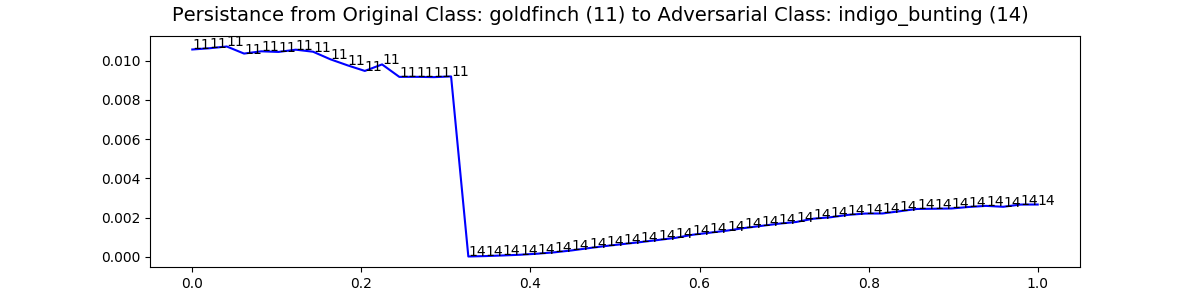
\includegraphics[width = \textwidth]
{c2_figures/persistence_interpolation-IMNET-class-11-vgg16-BIM-48-attack_data-001.png}
\caption{The $0.7$-persistence of images along the straight line path from an image in class \texttt{goldfinch} (11) to an adversarial image generated with BIM in the class \texttt{indigo\_bunting} (14) on a vgg16 classifier. The classification of each image on the straight line is listed as a number so that it is possible to see the transition from one class to another. The vertical axis is $0.7$-persistence and the horizontal axis is progress towards the adversarial image.}\label{fig:persistent_interpimage}
\end{figure}

An aggregation of persistence for many randomly selected images from the \texttt{goldfinch} class in the validation set for Imagenet are presented in Table \ref{TAB:PersistenceAlexVGG}. For each image of a \texttt{goldfinch} and for each network of alexnet and vgg16, attacks were prepared to a variety of 28 randomly selected targets using a BIM, MIFGSM, PGD, FGSM, R+FGSM, and CW attack strategies. The successful attacks were aggregated and their $0.7$-persistences were computed using the Bracketing Algorithm along with the $0.7$-persistences of the original images from which each attack was generated. Each attack strategy had a slightly different mixture of which source image and attack target combinations resulted in successful attacks. The overall rates for each are listed, as well as particular results on the most successful attack strategies in our experiments, BIM, MIFGSM, and PGD. The results indicate that adversarial images generated for these networks (alexnet and vgg16) using these attacks were less persistent, and hence less stable, than natural images for the same models. 


### kill

\begin{table}[ht]
\centering
\caption{The $0.7$-persistence values for natural (Nat) and adversarial (Adv) images along with average distortion for adversarial images of alexnet and vgg16 for attacks generated with BIM, MIFGSM, and PGD on images from class \texttt{goldfinch} targeted toward other classes from the ILSVRC 2015 classification labels.}
\label{TAB:PersistenceAlexVGG}
\begin{tabular}{llll}
\toprule
Network/Method & Avg Dist & Persist (Nat) & Persist (Adv) \\
\midrule
alexnet (total) & 0.0194 & 0.0155 & 0.0049 \\ 
\:\: BIM        & 0.0188 & 0.0162 & 0.0050 \\ 
\:\: MIFGSM     & 0.0240 & 0.0159 & 0.0053 \\ 
\:\: PGD        & 0.0188 & 0.0162 & 0.0050 \\ 
\midrule
vgg16   (total) & 0.0154 & 0.0146 & 0.0011 \\ 
\:\: BIM        & 0.0181 & 0.0145 & 0.0012 \\ 
\:\: MIFGSM     & 0.0238 & 0.0149 & 0.0018 \\ 
\:\: PGD        & 0.0181 & 0.0145 & 0.0012 \\ 
\bottomrule
\end{tabular}
\end{table}

% % figure showing natural image
% \begin{figure}[p]
% \centering
% \includegraphics[width = \textwidth]
% %[trim=200 80 100 10,width = .95\textwidth]
% %trim=200 80 100 100, clip,width=15cm]
% {sampling_histograms/samplot_test.png}
% %{c2_figures/Image918-O1Anone_varx40.png}
% %%% Creator: Matplotlib, PGF backend
%%
%% To include the figure in your LaTeX document, write
%%   \input{<filename>.pgf}
%%
%% Make sure the required packages are loaded in your preamble
%%   \usepackage{pgf}
%%
%% and, on pdftex
%%   \usepackage[utf8]{inputenc}\DeclareUnicodeCharacter{2212}{-}
%%
%% or, on luatex and xetex
%%   \usepackage{unicode-math}
%%
%% Figures using additional raster images can only be included by \input if
%% they are in the same directory as the main LaTeX file. For loading figures
%% from other directories you can use the `import` package
%%   \usepackage{import}
%%
%% and then include the figures with
%%   \import{<path to file>}{<filename>.pgf}
%%
%% Matplotlib used the following preamble
%%   \usepackage{fontspec}
%%   \setmainfont{DejaVuSerif.ttf}[Path=C:/Users/glickenstein/anaconda3/lib/site-packages/matplotlib/mpl-data/fonts/ttf/]
%%   \setsansfont{DejaVuSans.ttf}[Path=C:/Users/glickenstein/anaconda3/lib/site-packages/matplotlib/mpl-data/fonts/ttf/]
%%   \setmonofont{DejaVuSansMono.ttf}[Path=C:/Users/glickenstein/anaconda3/lib/site-packages/matplotlib/mpl-data/fonts/ttf/]
%%
\begingroup%
\makeatletter%
\begin{pgfpicture}%
\pgfpathrectangle{\pgfpointorigin}{\pgfqpoint{5.000000in}{2.500000in}}%
\pgfusepath{use as bounding box, clip}%
\begin{pgfscope}%
\pgfsetbuttcap%
\pgfsetmiterjoin%
\definecolor{currentfill}{rgb}{1.000000,1.000000,1.000000}%
\pgfsetfillcolor{currentfill}%
\pgfsetlinewidth{0.000000pt}%
\definecolor{currentstroke}{rgb}{1.000000,1.000000,1.000000}%
\pgfsetstrokecolor{currentstroke}%
\pgfsetdash{}{0pt}%
\pgfpathmoveto{\pgfqpoint{0.000000in}{0.000000in}}%
\pgfpathlineto{\pgfqpoint{5.000000in}{0.000000in}}%
\pgfpathlineto{\pgfqpoint{5.000000in}{2.500000in}}%
\pgfpathlineto{\pgfqpoint{0.000000in}{2.500000in}}%
\pgfpathclose%
\pgfusepath{fill}%
\end{pgfscope}%
\begin{pgfscope}%
\pgfsetbuttcap%
\pgfsetmiterjoin%
\definecolor{currentfill}{rgb}{1.000000,1.000000,1.000000}%
\pgfsetfillcolor{currentfill}%
\pgfsetlinewidth{0.000000pt}%
\definecolor{currentstroke}{rgb}{0.000000,0.000000,0.000000}%
\pgfsetstrokecolor{currentstroke}%
\pgfsetstrokeopacity{0.000000}%
\pgfsetdash{}{0pt}%
\pgfpathmoveto{\pgfqpoint{0.300000in}{1.350000in}}%
\pgfpathlineto{\pgfqpoint{4.950000in}{1.350000in}}%
\pgfpathlineto{\pgfqpoint{4.950000in}{2.475000in}}%
\pgfpathlineto{\pgfqpoint{0.300000in}{2.475000in}}%
\pgfpathclose%
\pgfusepath{fill}%
\end{pgfscope}%
\begin{pgfscope}%
\pgfsetbuttcap%
\pgfsetroundjoin%
\definecolor{currentfill}{rgb}{0.000000,0.000000,0.000000}%
\pgfsetfillcolor{currentfill}%
\pgfsetlinewidth{0.803000pt}%
\definecolor{currentstroke}{rgb}{0.000000,0.000000,0.000000}%
\pgfsetstrokecolor{currentstroke}%
\pgfsetdash{}{0pt}%
\pgfsys@defobject{currentmarker}{\pgfqpoint{0.000000in}{-0.048611in}}{\pgfqpoint{0.000000in}{0.000000in}}{%
\pgfpathmoveto{\pgfqpoint{0.000000in}{0.000000in}}%
\pgfpathlineto{\pgfqpoint{0.000000in}{-0.048611in}}%
\pgfusepath{stroke,fill}%
}%
\begin{pgfscope}%
\pgfsys@transformshift{0.511364in}{1.350000in}%
\pgfsys@useobject{currentmarker}{}%
\end{pgfscope}%
\end{pgfscope}%
\begin{pgfscope}%
\definecolor{textcolor}{rgb}{0.000000,0.000000,0.000000}%
\pgfsetstrokecolor{textcolor}%
\pgfsetfillcolor{textcolor}%
\pgftext[x=0.511364in,y=1.252778in,,top]{\color{textcolor}\sffamily\fontsize{16.000000}{19.200000}\selectfont 0.0}%
\end{pgfscope}%
\begin{pgfscope}%
\pgfsetbuttcap%
\pgfsetroundjoin%
\definecolor{currentfill}{rgb}{0.000000,0.000000,0.000000}%
\pgfsetfillcolor{currentfill}%
\pgfsetlinewidth{0.803000pt}%
\definecolor{currentstroke}{rgb}{0.000000,0.000000,0.000000}%
\pgfsetstrokecolor{currentstroke}%
\pgfsetdash{}{0pt}%
\pgfsys@defobject{currentmarker}{\pgfqpoint{0.000000in}{-0.048611in}}{\pgfqpoint{0.000000in}{0.000000in}}{%
\pgfpathmoveto{\pgfqpoint{0.000000in}{0.000000in}}%
\pgfpathlineto{\pgfqpoint{0.000000in}{-0.048611in}}%
\pgfusepath{stroke,fill}%
}%
\begin{pgfscope}%
\pgfsys@transformshift{1.356818in}{1.350000in}%
\pgfsys@useobject{currentmarker}{}%
\end{pgfscope}%
\end{pgfscope}%
\begin{pgfscope}%
\definecolor{textcolor}{rgb}{0.000000,0.000000,0.000000}%
\pgfsetstrokecolor{textcolor}%
\pgfsetfillcolor{textcolor}%
\pgftext[x=1.356818in,y=1.252778in,,top]{\color{textcolor}\sffamily\fontsize{16.000000}{19.200000}\selectfont 0.2}%
\end{pgfscope}%
\begin{pgfscope}%
\pgfsetbuttcap%
\pgfsetroundjoin%
\definecolor{currentfill}{rgb}{0.000000,0.000000,0.000000}%
\pgfsetfillcolor{currentfill}%
\pgfsetlinewidth{0.803000pt}%
\definecolor{currentstroke}{rgb}{0.000000,0.000000,0.000000}%
\pgfsetstrokecolor{currentstroke}%
\pgfsetdash{}{0pt}%
\pgfsys@defobject{currentmarker}{\pgfqpoint{0.000000in}{-0.048611in}}{\pgfqpoint{0.000000in}{0.000000in}}{%
\pgfpathmoveto{\pgfqpoint{0.000000in}{0.000000in}}%
\pgfpathlineto{\pgfqpoint{0.000000in}{-0.048611in}}%
\pgfusepath{stroke,fill}%
}%
\begin{pgfscope}%
\pgfsys@transformshift{2.202273in}{1.350000in}%
\pgfsys@useobject{currentmarker}{}%
\end{pgfscope}%
\end{pgfscope}%
\begin{pgfscope}%
\definecolor{textcolor}{rgb}{0.000000,0.000000,0.000000}%
\pgfsetstrokecolor{textcolor}%
\pgfsetfillcolor{textcolor}%
\pgftext[x=2.202273in,y=1.252778in,,top]{\color{textcolor}\sffamily\fontsize{16.000000}{19.200000}\selectfont 0.4}%
\end{pgfscope}%
\begin{pgfscope}%
\pgfsetbuttcap%
\pgfsetroundjoin%
\definecolor{currentfill}{rgb}{0.000000,0.000000,0.000000}%
\pgfsetfillcolor{currentfill}%
\pgfsetlinewidth{0.803000pt}%
\definecolor{currentstroke}{rgb}{0.000000,0.000000,0.000000}%
\pgfsetstrokecolor{currentstroke}%
\pgfsetdash{}{0pt}%
\pgfsys@defobject{currentmarker}{\pgfqpoint{0.000000in}{-0.048611in}}{\pgfqpoint{0.000000in}{0.000000in}}{%
\pgfpathmoveto{\pgfqpoint{0.000000in}{0.000000in}}%
\pgfpathlineto{\pgfqpoint{0.000000in}{-0.048611in}}%
\pgfusepath{stroke,fill}%
}%
\begin{pgfscope}%
\pgfsys@transformshift{3.047727in}{1.350000in}%
\pgfsys@useobject{currentmarker}{}%
\end{pgfscope}%
\end{pgfscope}%
\begin{pgfscope}%
\definecolor{textcolor}{rgb}{0.000000,0.000000,0.000000}%
\pgfsetstrokecolor{textcolor}%
\pgfsetfillcolor{textcolor}%
\pgftext[x=3.047727in,y=1.252778in,,top]{\color{textcolor}\sffamily\fontsize{16.000000}{19.200000}\selectfont 0.6}%
\end{pgfscope}%
\begin{pgfscope}%
\pgfsetbuttcap%
\pgfsetroundjoin%
\definecolor{currentfill}{rgb}{0.000000,0.000000,0.000000}%
\pgfsetfillcolor{currentfill}%
\pgfsetlinewidth{0.803000pt}%
\definecolor{currentstroke}{rgb}{0.000000,0.000000,0.000000}%
\pgfsetstrokecolor{currentstroke}%
\pgfsetdash{}{0pt}%
\pgfsys@defobject{currentmarker}{\pgfqpoint{0.000000in}{-0.048611in}}{\pgfqpoint{0.000000in}{0.000000in}}{%
\pgfpathmoveto{\pgfqpoint{0.000000in}{0.000000in}}%
\pgfpathlineto{\pgfqpoint{0.000000in}{-0.048611in}}%
\pgfusepath{stroke,fill}%
}%
\begin{pgfscope}%
\pgfsys@transformshift{3.893182in}{1.350000in}%
\pgfsys@useobject{currentmarker}{}%
\end{pgfscope}%
\end{pgfscope}%
\begin{pgfscope}%
\definecolor{textcolor}{rgb}{0.000000,0.000000,0.000000}%
\pgfsetstrokecolor{textcolor}%
\pgfsetfillcolor{textcolor}%
\pgftext[x=3.893182in,y=1.252778in,,top]{\color{textcolor}\sffamily\fontsize{16.000000}{19.200000}\selectfont 0.8}%
\end{pgfscope}%
\begin{pgfscope}%
\pgfsetbuttcap%
\pgfsetroundjoin%
\definecolor{currentfill}{rgb}{0.000000,0.000000,0.000000}%
\pgfsetfillcolor{currentfill}%
\pgfsetlinewidth{0.803000pt}%
\definecolor{currentstroke}{rgb}{0.000000,0.000000,0.000000}%
\pgfsetstrokecolor{currentstroke}%
\pgfsetdash{}{0pt}%
\pgfsys@defobject{currentmarker}{\pgfqpoint{0.000000in}{-0.048611in}}{\pgfqpoint{0.000000in}{0.000000in}}{%
\pgfpathmoveto{\pgfqpoint{0.000000in}{0.000000in}}%
\pgfpathlineto{\pgfqpoint{0.000000in}{-0.048611in}}%
\pgfusepath{stroke,fill}%
}%
\begin{pgfscope}%
\pgfsys@transformshift{4.738636in}{1.350000in}%
\pgfsys@useobject{currentmarker}{}%
\end{pgfscope}%
\end{pgfscope}%
\begin{pgfscope}%
\definecolor{textcolor}{rgb}{0.000000,0.000000,0.000000}%
\pgfsetstrokecolor{textcolor}%
\pgfsetfillcolor{textcolor}%
\pgftext[x=4.738636in,y=1.252778in,,top]{\color{textcolor}\sffamily\fontsize{16.000000}{19.200000}\selectfont 1.0}%
\end{pgfscope}%
\begin{pgfscope}%
\definecolor{textcolor}{rgb}{0.000000,0.000000,0.000000}%
\pgfsetstrokecolor{textcolor}%
\pgfsetfillcolor{textcolor}%
\pgftext[x=2.625000in,y=0.982162in,,top]{\color{textcolor}\sffamily\fontsize{16.000000}{19.200000}\selectfont Standard Deviation (\(\displaystyle \sigma\))}%
\end{pgfscope}%
\begin{pgfscope}%
\pgfsetbuttcap%
\pgfsetroundjoin%
\definecolor{currentfill}{rgb}{0.000000,0.000000,0.000000}%
\pgfsetfillcolor{currentfill}%
\pgfsetlinewidth{0.803000pt}%
\definecolor{currentstroke}{rgb}{0.000000,0.000000,0.000000}%
\pgfsetstrokecolor{currentstroke}%
\pgfsetdash{}{0pt}%
\pgfsys@defobject{currentmarker}{\pgfqpoint{-0.048611in}{0.000000in}}{\pgfqpoint{0.000000in}{0.000000in}}{%
\pgfpathmoveto{\pgfqpoint{0.000000in}{0.000000in}}%
\pgfpathlineto{\pgfqpoint{-0.048611in}{0.000000in}}%
\pgfusepath{stroke,fill}%
}%
\begin{pgfscope}%
\pgfsys@transformshift{0.300000in}{1.401136in}%
\pgfsys@useobject{currentmarker}{}%
\end{pgfscope}%
\end{pgfscope}%
\begin{pgfscope}%
\definecolor{textcolor}{rgb}{0.000000,0.000000,0.000000}%
\pgfsetstrokecolor{textcolor}%
\pgfsetfillcolor{textcolor}%
\pgftext[x=0.061393in, y=1.316718in, left, base]{\color{textcolor}\sffamily\fontsize{16.000000}{19.200000}\selectfont 0}%
\end{pgfscope}%
\begin{pgfscope}%
\pgfsetbuttcap%
\pgfsetroundjoin%
\definecolor{currentfill}{rgb}{0.000000,0.000000,0.000000}%
\pgfsetfillcolor{currentfill}%
\pgfsetlinewidth{0.803000pt}%
\definecolor{currentstroke}{rgb}{0.000000,0.000000,0.000000}%
\pgfsetstrokecolor{currentstroke}%
\pgfsetdash{}{0pt}%
\pgfsys@defobject{currentmarker}{\pgfqpoint{-0.048611in}{0.000000in}}{\pgfqpoint{0.000000in}{0.000000in}}{%
\pgfpathmoveto{\pgfqpoint{0.000000in}{0.000000in}}%
\pgfpathlineto{\pgfqpoint{-0.048611in}{0.000000in}}%
\pgfusepath{stroke,fill}%
}%
\begin{pgfscope}%
\pgfsys@transformshift{0.300000in}{2.423864in}%
\pgfsys@useobject{currentmarker}{}%
\end{pgfscope}%
\end{pgfscope}%
\begin{pgfscope}%
\definecolor{textcolor}{rgb}{0.000000,0.000000,0.000000}%
\pgfsetstrokecolor{textcolor}%
\pgfsetfillcolor{textcolor}%
\pgftext[x=-0.221376in, y=2.339445in, left, base]{\color{textcolor}\sffamily\fontsize{16.000000}{19.200000}\selectfont 100}%
\end{pgfscope}%
\begin{pgfscope}%
\definecolor{textcolor}{rgb}{0.000000,0.000000,0.000000}%
\pgfsetstrokecolor{textcolor}%
\pgfsetfillcolor{textcolor}%
\pgftext[x=-0.151931in,y=1.912500in,,bottom,rotate=90.000000]{\color{textcolor}\sffamily\fontsize{16.000000}{19.200000}\selectfont Count}%
\end{pgfscope}%
\begin{pgfscope}%
\pgfpathrectangle{\pgfqpoint{0.300000in}{1.350000in}}{\pgfqpoint{4.650000in}{1.125000in}}%
\pgfusepath{clip}%
\pgfsetrectcap%
\pgfsetroundjoin%
\pgfsetlinewidth{1.003750pt}%
\definecolor{currentstroke}{rgb}{0.000000,0.000000,1.000000}%
\pgfsetstrokecolor{currentstroke}%
\pgfsetstrokeopacity{0.200000}%
\pgfsetdash{}{0pt}%
\pgfpathmoveto{\pgfqpoint{0.511364in}{1.401136in}}%
\pgfpathlineto{\pgfqpoint{2.848047in}{1.401136in}}%
\pgfpathlineto{\pgfqpoint{2.869290in}{1.411364in}}%
\pgfpathlineto{\pgfqpoint{2.890532in}{1.401136in}}%
\pgfpathlineto{\pgfqpoint{2.954260in}{1.401136in}}%
\pgfpathlineto{\pgfqpoint{2.996745in}{1.421591in}}%
\pgfpathlineto{\pgfqpoint{3.017988in}{1.401136in}}%
\pgfpathlineto{\pgfqpoint{3.039230in}{1.401136in}}%
\pgfpathlineto{\pgfqpoint{3.060473in}{1.411364in}}%
\pgfpathlineto{\pgfqpoint{3.081715in}{1.401136in}}%
\pgfpathlineto{\pgfqpoint{3.102958in}{1.401136in}}%
\pgfpathlineto{\pgfqpoint{3.124201in}{1.411364in}}%
\pgfpathlineto{\pgfqpoint{3.145443in}{1.401136in}}%
\pgfpathlineto{\pgfqpoint{3.357869in}{1.401136in}}%
\pgfpathlineto{\pgfqpoint{3.379111in}{1.421591in}}%
\pgfpathlineto{\pgfqpoint{3.400354in}{1.401136in}}%
\pgfpathlineto{\pgfqpoint{3.506567in}{1.401136in}}%
\pgfpathlineto{\pgfqpoint{3.527810in}{1.411364in}}%
\pgfpathlineto{\pgfqpoint{3.549052in}{1.401136in}}%
\pgfpathlineto{\pgfqpoint{3.634022in}{1.401136in}}%
\pgfpathlineto{\pgfqpoint{3.655265in}{1.411364in}}%
\pgfpathlineto{\pgfqpoint{3.676508in}{1.401136in}}%
\pgfpathlineto{\pgfqpoint{3.697750in}{1.431818in}}%
\pgfpathlineto{\pgfqpoint{3.761478in}{1.401136in}}%
\pgfpathlineto{\pgfqpoint{3.782720in}{1.431818in}}%
\pgfpathlineto{\pgfqpoint{3.803963in}{1.401136in}}%
\pgfpathlineto{\pgfqpoint{3.825206in}{1.401136in}}%
\pgfpathlineto{\pgfqpoint{3.846448in}{1.411364in}}%
\pgfpathlineto{\pgfqpoint{3.867691in}{1.401136in}}%
\pgfpathlineto{\pgfqpoint{3.888933in}{1.411364in}}%
\pgfpathlineto{\pgfqpoint{3.910176in}{1.401136in}}%
\pgfpathlineto{\pgfqpoint{3.931418in}{1.411364in}}%
\pgfpathlineto{\pgfqpoint{3.952661in}{1.401136in}}%
\pgfpathlineto{\pgfqpoint{3.973904in}{1.421591in}}%
\pgfpathlineto{\pgfqpoint{3.995146in}{1.421591in}}%
\pgfpathlineto{\pgfqpoint{4.016389in}{1.411364in}}%
\pgfpathlineto{\pgfqpoint{4.037631in}{1.411364in}}%
\pgfpathlineto{\pgfqpoint{4.058874in}{1.401136in}}%
\pgfpathlineto{\pgfqpoint{4.080116in}{1.411364in}}%
\pgfpathlineto{\pgfqpoint{4.101359in}{1.401136in}}%
\pgfpathlineto{\pgfqpoint{4.122602in}{1.411364in}}%
\pgfpathlineto{\pgfqpoint{4.143844in}{1.431818in}}%
\pgfpathlineto{\pgfqpoint{4.165087in}{1.421591in}}%
\pgfpathlineto{\pgfqpoint{4.186329in}{1.421591in}}%
\pgfpathlineto{\pgfqpoint{4.207572in}{1.401136in}}%
\pgfpathlineto{\pgfqpoint{4.228815in}{1.401136in}}%
\pgfpathlineto{\pgfqpoint{4.250057in}{1.421591in}}%
\pgfpathlineto{\pgfqpoint{4.271300in}{1.421591in}}%
\pgfpathlineto{\pgfqpoint{4.292542in}{1.401136in}}%
\pgfpathlineto{\pgfqpoint{4.313785in}{1.411364in}}%
\pgfpathlineto{\pgfqpoint{4.335027in}{1.411364in}}%
\pgfpathlineto{\pgfqpoint{4.356270in}{1.421591in}}%
\pgfpathlineto{\pgfqpoint{4.377513in}{1.411364in}}%
\pgfpathlineto{\pgfqpoint{4.398755in}{1.421591in}}%
\pgfpathlineto{\pgfqpoint{4.419998in}{1.411364in}}%
\pgfpathlineto{\pgfqpoint{4.441240in}{1.411364in}}%
\pgfpathlineto{\pgfqpoint{4.462483in}{1.442045in}}%
\pgfpathlineto{\pgfqpoint{4.483725in}{1.421591in}}%
\pgfpathlineto{\pgfqpoint{4.504968in}{1.442045in}}%
\pgfpathlineto{\pgfqpoint{4.526211in}{1.401136in}}%
\pgfpathlineto{\pgfqpoint{4.547453in}{1.401136in}}%
\pgfpathlineto{\pgfqpoint{4.568696in}{1.431818in}}%
\pgfpathlineto{\pgfqpoint{4.589938in}{1.421591in}}%
\pgfpathlineto{\pgfqpoint{4.611181in}{1.421591in}}%
\pgfpathlineto{\pgfqpoint{4.632423in}{1.401136in}}%
\pgfpathlineto{\pgfqpoint{4.674909in}{1.442045in}}%
\pgfpathlineto{\pgfqpoint{4.696151in}{1.421591in}}%
\pgfpathlineto{\pgfqpoint{4.717394in}{1.421591in}}%
\pgfpathlineto{\pgfqpoint{4.738636in}{1.431818in}}%
\pgfpathlineto{\pgfqpoint{4.738636in}{1.431818in}}%
\pgfusepath{stroke}%
\end{pgfscope}%
\begin{pgfscope}%
\pgfpathrectangle{\pgfqpoint{0.300000in}{1.350000in}}{\pgfqpoint{4.650000in}{1.125000in}}%
\pgfusepath{clip}%
\pgfsetrectcap%
\pgfsetroundjoin%
\pgfsetlinewidth{1.003750pt}%
\definecolor{currentstroke}{rgb}{0.000000,0.000000,1.000000}%
\pgfsetstrokecolor{currentstroke}%
\pgfsetstrokeopacity{0.200000}%
\pgfsetdash{}{0pt}%
\pgfpathmoveto{\pgfqpoint{0.511364in}{1.401136in}}%
\pgfpathlineto{\pgfqpoint{3.187928in}{1.401136in}}%
\pgfpathlineto{\pgfqpoint{3.209171in}{1.411364in}}%
\pgfpathlineto{\pgfqpoint{3.230413in}{1.401136in}}%
\pgfpathlineto{\pgfqpoint{4.165087in}{1.401136in}}%
\pgfpathlineto{\pgfqpoint{4.186329in}{1.411364in}}%
\pgfpathlineto{\pgfqpoint{4.207572in}{1.401136in}}%
\pgfpathlineto{\pgfqpoint{4.377513in}{1.401136in}}%
\pgfpathlineto{\pgfqpoint{4.398755in}{1.411364in}}%
\pgfpathlineto{\pgfqpoint{4.419998in}{1.401136in}}%
\pgfpathlineto{\pgfqpoint{4.738636in}{1.401136in}}%
\pgfpathlineto{\pgfqpoint{4.738636in}{1.401136in}}%
\pgfusepath{stroke}%
\end{pgfscope}%
\begin{pgfscope}%
\pgfpathrectangle{\pgfqpoint{0.300000in}{1.350000in}}{\pgfqpoint{4.650000in}{1.125000in}}%
\pgfusepath{clip}%
\pgfsetrectcap%
\pgfsetroundjoin%
\pgfsetlinewidth{1.003750pt}%
\definecolor{currentstroke}{rgb}{0.000000,0.000000,1.000000}%
\pgfsetstrokecolor{currentstroke}%
\pgfsetstrokeopacity{0.200000}%
\pgfsetdash{}{0pt}%
\pgfpathmoveto{\pgfqpoint{0.511364in}{1.401136in}}%
\pgfpathlineto{\pgfqpoint{0.638819in}{1.401136in}}%
\pgfpathlineto{\pgfqpoint{0.660062in}{1.462500in}}%
\pgfpathlineto{\pgfqpoint{0.681304in}{1.503409in}}%
\pgfpathlineto{\pgfqpoint{0.702547in}{1.667045in}}%
\pgfpathlineto{\pgfqpoint{0.723789in}{1.769318in}}%
\pgfpathlineto{\pgfqpoint{0.766275in}{1.912500in}}%
\pgfpathlineto{\pgfqpoint{0.787517in}{1.973864in}}%
\pgfpathlineto{\pgfqpoint{0.808760in}{2.055682in}}%
\pgfpathlineto{\pgfqpoint{0.830002in}{2.004545in}}%
\pgfpathlineto{\pgfqpoint{0.851245in}{2.086364in}}%
\pgfpathlineto{\pgfqpoint{0.872487in}{2.076136in}}%
\pgfpathlineto{\pgfqpoint{0.893730in}{2.106818in}}%
\pgfpathlineto{\pgfqpoint{0.914973in}{2.076136in}}%
\pgfpathlineto{\pgfqpoint{0.936215in}{2.127273in}}%
\pgfpathlineto{\pgfqpoint{0.957458in}{2.076136in}}%
\pgfpathlineto{\pgfqpoint{0.978700in}{2.127273in}}%
\pgfpathlineto{\pgfqpoint{0.999943in}{2.106818in}}%
\pgfpathlineto{\pgfqpoint{1.021185in}{2.168182in}}%
\pgfpathlineto{\pgfqpoint{1.042428in}{2.250000in}}%
\pgfpathlineto{\pgfqpoint{1.063671in}{2.137500in}}%
\pgfpathlineto{\pgfqpoint{1.084913in}{2.096591in}}%
\pgfpathlineto{\pgfqpoint{1.106156in}{2.147727in}}%
\pgfpathlineto{\pgfqpoint{1.127398in}{2.147727in}}%
\pgfpathlineto{\pgfqpoint{1.148641in}{2.045455in}}%
\pgfpathlineto{\pgfqpoint{1.169884in}{2.219318in}}%
\pgfpathlineto{\pgfqpoint{1.191126in}{2.127273in}}%
\pgfpathlineto{\pgfqpoint{1.212369in}{2.168182in}}%
\pgfpathlineto{\pgfqpoint{1.233611in}{2.168182in}}%
\pgfpathlineto{\pgfqpoint{1.254854in}{2.127273in}}%
\pgfpathlineto{\pgfqpoint{1.276096in}{2.096591in}}%
\pgfpathlineto{\pgfqpoint{1.297339in}{2.035227in}}%
\pgfpathlineto{\pgfqpoint{1.318582in}{2.127273in}}%
\pgfpathlineto{\pgfqpoint{1.339824in}{2.076136in}}%
\pgfpathlineto{\pgfqpoint{1.361067in}{2.086364in}}%
\pgfpathlineto{\pgfqpoint{1.382309in}{2.035227in}}%
\pgfpathlineto{\pgfqpoint{1.403552in}{1.922727in}}%
\pgfpathlineto{\pgfqpoint{1.424794in}{1.892045in}}%
\pgfpathlineto{\pgfqpoint{1.446037in}{1.932955in}}%
\pgfpathlineto{\pgfqpoint{1.467280in}{2.014773in}}%
\pgfpathlineto{\pgfqpoint{1.488522in}{1.820455in}}%
\pgfpathlineto{\pgfqpoint{1.509765in}{1.861364in}}%
\pgfpathlineto{\pgfqpoint{1.531007in}{1.892045in}}%
\pgfpathlineto{\pgfqpoint{1.552250in}{1.789773in}}%
\pgfpathlineto{\pgfqpoint{1.573492in}{1.810227in}}%
\pgfpathlineto{\pgfqpoint{1.594735in}{1.779545in}}%
\pgfpathlineto{\pgfqpoint{1.615978in}{1.759091in}}%
\pgfpathlineto{\pgfqpoint{1.637220in}{1.707955in}}%
\pgfpathlineto{\pgfqpoint{1.658463in}{1.759091in}}%
\pgfpathlineto{\pgfqpoint{1.679705in}{1.738636in}}%
\pgfpathlineto{\pgfqpoint{1.700948in}{1.881818in}}%
\pgfpathlineto{\pgfqpoint{1.722190in}{1.738636in}}%
\pgfpathlineto{\pgfqpoint{1.743433in}{1.789773in}}%
\pgfpathlineto{\pgfqpoint{1.764676in}{1.738636in}}%
\pgfpathlineto{\pgfqpoint{1.785918in}{1.636364in}}%
\pgfpathlineto{\pgfqpoint{1.807161in}{1.626136in}}%
\pgfpathlineto{\pgfqpoint{1.849646in}{1.687500in}}%
\pgfpathlineto{\pgfqpoint{1.870889in}{1.707955in}}%
\pgfpathlineto{\pgfqpoint{1.892131in}{1.687500in}}%
\pgfpathlineto{\pgfqpoint{1.913374in}{1.677273in}}%
\pgfpathlineto{\pgfqpoint{1.934616in}{1.677273in}}%
\pgfpathlineto{\pgfqpoint{1.955859in}{1.667045in}}%
\pgfpathlineto{\pgfqpoint{1.977101in}{1.605682in}}%
\pgfpathlineto{\pgfqpoint{1.998344in}{1.646591in}}%
\pgfpathlineto{\pgfqpoint{2.019587in}{1.605682in}}%
\pgfpathlineto{\pgfqpoint{2.040829in}{1.636364in}}%
\pgfpathlineto{\pgfqpoint{2.062072in}{1.615909in}}%
\pgfpathlineto{\pgfqpoint{2.083314in}{1.605682in}}%
\pgfpathlineto{\pgfqpoint{2.104557in}{1.656818in}}%
\pgfpathlineto{\pgfqpoint{2.125799in}{1.595455in}}%
\pgfpathlineto{\pgfqpoint{2.147042in}{1.646591in}}%
\pgfpathlineto{\pgfqpoint{2.168285in}{1.564773in}}%
\pgfpathlineto{\pgfqpoint{2.189527in}{1.615909in}}%
\pgfpathlineto{\pgfqpoint{2.210770in}{1.544318in}}%
\pgfpathlineto{\pgfqpoint{2.232012in}{1.523864in}}%
\pgfpathlineto{\pgfqpoint{2.253255in}{1.605682in}}%
\pgfpathlineto{\pgfqpoint{2.274497in}{1.544318in}}%
\pgfpathlineto{\pgfqpoint{2.295740in}{1.585227in}}%
\pgfpathlineto{\pgfqpoint{2.316983in}{1.615909in}}%
\pgfpathlineto{\pgfqpoint{2.338225in}{1.605682in}}%
\pgfpathlineto{\pgfqpoint{2.359468in}{1.646591in}}%
\pgfpathlineto{\pgfqpoint{2.380710in}{1.615909in}}%
\pgfpathlineto{\pgfqpoint{2.401953in}{1.595455in}}%
\pgfpathlineto{\pgfqpoint{2.423196in}{1.554545in}}%
\pgfpathlineto{\pgfqpoint{2.444438in}{1.595455in}}%
\pgfpathlineto{\pgfqpoint{2.465681in}{1.523864in}}%
\pgfpathlineto{\pgfqpoint{2.486923in}{1.482955in}}%
\pgfpathlineto{\pgfqpoint{2.508166in}{1.554545in}}%
\pgfpathlineto{\pgfqpoint{2.529408in}{1.534091in}}%
\pgfpathlineto{\pgfqpoint{2.550651in}{1.595455in}}%
\pgfpathlineto{\pgfqpoint{2.571894in}{1.554545in}}%
\pgfpathlineto{\pgfqpoint{2.593136in}{1.482955in}}%
\pgfpathlineto{\pgfqpoint{2.614379in}{1.513636in}}%
\pgfpathlineto{\pgfqpoint{2.635621in}{1.554545in}}%
\pgfpathlineto{\pgfqpoint{2.656864in}{1.482955in}}%
\pgfpathlineto{\pgfqpoint{2.678106in}{1.595455in}}%
\pgfpathlineto{\pgfqpoint{2.699349in}{1.503409in}}%
\pgfpathlineto{\pgfqpoint{2.720592in}{1.503409in}}%
\pgfpathlineto{\pgfqpoint{2.741834in}{1.513636in}}%
\pgfpathlineto{\pgfqpoint{2.763077in}{1.544318in}}%
\pgfpathlineto{\pgfqpoint{2.784319in}{1.544318in}}%
\pgfpathlineto{\pgfqpoint{2.805562in}{1.513636in}}%
\pgfpathlineto{\pgfqpoint{2.826804in}{1.513636in}}%
\pgfpathlineto{\pgfqpoint{2.848047in}{1.472727in}}%
\pgfpathlineto{\pgfqpoint{2.869290in}{1.503409in}}%
\pgfpathlineto{\pgfqpoint{2.890532in}{1.544318in}}%
\pgfpathlineto{\pgfqpoint{2.911775in}{1.503409in}}%
\pgfpathlineto{\pgfqpoint{2.933017in}{1.513636in}}%
\pgfpathlineto{\pgfqpoint{2.954260in}{1.452273in}}%
\pgfpathlineto{\pgfqpoint{2.996745in}{1.472727in}}%
\pgfpathlineto{\pgfqpoint{3.017988in}{1.503409in}}%
\pgfpathlineto{\pgfqpoint{3.039230in}{1.462500in}}%
\pgfpathlineto{\pgfqpoint{3.060473in}{1.523864in}}%
\pgfpathlineto{\pgfqpoint{3.081715in}{1.462500in}}%
\pgfpathlineto{\pgfqpoint{3.102958in}{1.534091in}}%
\pgfpathlineto{\pgfqpoint{3.124201in}{1.482955in}}%
\pgfpathlineto{\pgfqpoint{3.145443in}{1.482955in}}%
\pgfpathlineto{\pgfqpoint{3.166686in}{1.472727in}}%
\pgfpathlineto{\pgfqpoint{3.187928in}{1.482955in}}%
\pgfpathlineto{\pgfqpoint{3.209171in}{1.503409in}}%
\pgfpathlineto{\pgfqpoint{3.230413in}{1.462500in}}%
\pgfpathlineto{\pgfqpoint{3.251656in}{1.442045in}}%
\pgfpathlineto{\pgfqpoint{3.272899in}{1.482955in}}%
\pgfpathlineto{\pgfqpoint{3.294141in}{1.462500in}}%
\pgfpathlineto{\pgfqpoint{3.315384in}{1.493182in}}%
\pgfpathlineto{\pgfqpoint{3.336626in}{1.462500in}}%
\pgfpathlineto{\pgfqpoint{3.357869in}{1.462500in}}%
\pgfpathlineto{\pgfqpoint{3.379111in}{1.431818in}}%
\pgfpathlineto{\pgfqpoint{3.400354in}{1.421591in}}%
\pgfpathlineto{\pgfqpoint{3.421597in}{1.462500in}}%
\pgfpathlineto{\pgfqpoint{3.442839in}{1.472727in}}%
\pgfpathlineto{\pgfqpoint{3.464082in}{1.442045in}}%
\pgfpathlineto{\pgfqpoint{3.485324in}{1.462500in}}%
\pgfpathlineto{\pgfqpoint{3.506567in}{1.452273in}}%
\pgfpathlineto{\pgfqpoint{3.527810in}{1.421591in}}%
\pgfpathlineto{\pgfqpoint{3.549052in}{1.431818in}}%
\pgfpathlineto{\pgfqpoint{3.570295in}{1.462500in}}%
\pgfpathlineto{\pgfqpoint{3.591537in}{1.431818in}}%
\pgfpathlineto{\pgfqpoint{3.612780in}{1.411364in}}%
\pgfpathlineto{\pgfqpoint{3.634022in}{1.452273in}}%
\pgfpathlineto{\pgfqpoint{3.655265in}{1.442045in}}%
\pgfpathlineto{\pgfqpoint{3.676508in}{1.472727in}}%
\pgfpathlineto{\pgfqpoint{3.697750in}{1.452273in}}%
\pgfpathlineto{\pgfqpoint{3.718993in}{1.421591in}}%
\pgfpathlineto{\pgfqpoint{3.740235in}{1.411364in}}%
\pgfpathlineto{\pgfqpoint{3.761478in}{1.442045in}}%
\pgfpathlineto{\pgfqpoint{3.782720in}{1.452273in}}%
\pgfpathlineto{\pgfqpoint{3.803963in}{1.421591in}}%
\pgfpathlineto{\pgfqpoint{3.825206in}{1.401136in}}%
\pgfpathlineto{\pgfqpoint{3.846448in}{1.411364in}}%
\pgfpathlineto{\pgfqpoint{3.867691in}{1.431818in}}%
\pgfpathlineto{\pgfqpoint{3.888933in}{1.411364in}}%
\pgfpathlineto{\pgfqpoint{3.910176in}{1.442045in}}%
\pgfpathlineto{\pgfqpoint{3.931418in}{1.421591in}}%
\pgfpathlineto{\pgfqpoint{3.952661in}{1.442045in}}%
\pgfpathlineto{\pgfqpoint{3.973904in}{1.411364in}}%
\pgfpathlineto{\pgfqpoint{3.995146in}{1.421591in}}%
\pgfpathlineto{\pgfqpoint{4.016389in}{1.442045in}}%
\pgfpathlineto{\pgfqpoint{4.058874in}{1.421591in}}%
\pgfpathlineto{\pgfqpoint{4.080116in}{1.431818in}}%
\pgfpathlineto{\pgfqpoint{4.101359in}{1.421591in}}%
\pgfpathlineto{\pgfqpoint{4.122602in}{1.421591in}}%
\pgfpathlineto{\pgfqpoint{4.143844in}{1.431818in}}%
\pgfpathlineto{\pgfqpoint{4.165087in}{1.411364in}}%
\pgfpathlineto{\pgfqpoint{4.186329in}{1.421591in}}%
\pgfpathlineto{\pgfqpoint{4.207572in}{1.401136in}}%
\pgfpathlineto{\pgfqpoint{4.228815in}{1.411364in}}%
\pgfpathlineto{\pgfqpoint{4.250057in}{1.431818in}}%
\pgfpathlineto{\pgfqpoint{4.271300in}{1.401136in}}%
\pgfpathlineto{\pgfqpoint{4.292542in}{1.411364in}}%
\pgfpathlineto{\pgfqpoint{4.313785in}{1.401136in}}%
\pgfpathlineto{\pgfqpoint{4.335027in}{1.411364in}}%
\pgfpathlineto{\pgfqpoint{4.356270in}{1.401136in}}%
\pgfpathlineto{\pgfqpoint{4.377513in}{1.411364in}}%
\pgfpathlineto{\pgfqpoint{4.398755in}{1.411364in}}%
\pgfpathlineto{\pgfqpoint{4.419998in}{1.421591in}}%
\pgfpathlineto{\pgfqpoint{4.441240in}{1.401136in}}%
\pgfpathlineto{\pgfqpoint{4.504968in}{1.401136in}}%
\pgfpathlineto{\pgfqpoint{4.526211in}{1.411364in}}%
\pgfpathlineto{\pgfqpoint{4.547453in}{1.411364in}}%
\pgfpathlineto{\pgfqpoint{4.568696in}{1.401136in}}%
\pgfpathlineto{\pgfqpoint{4.589938in}{1.401136in}}%
\pgfpathlineto{\pgfqpoint{4.611181in}{1.411364in}}%
\pgfpathlineto{\pgfqpoint{4.632423in}{1.401136in}}%
\pgfpathlineto{\pgfqpoint{4.717394in}{1.401136in}}%
\pgfpathlineto{\pgfqpoint{4.738636in}{1.411364in}}%
\pgfpathlineto{\pgfqpoint{4.738636in}{1.411364in}}%
\pgfusepath{stroke}%
\end{pgfscope}%
\begin{pgfscope}%
\pgfpathrectangle{\pgfqpoint{0.300000in}{1.350000in}}{\pgfqpoint{4.650000in}{1.125000in}}%
\pgfusepath{clip}%
\pgfsetrectcap%
\pgfsetroundjoin%
\pgfsetlinewidth{1.003750pt}%
\definecolor{currentstroke}{rgb}{0.000000,0.000000,1.000000}%
\pgfsetstrokecolor{currentstroke}%
\pgfsetstrokeopacity{0.200000}%
\pgfsetdash{}{0pt}%
\pgfpathmoveto{\pgfqpoint{0.511364in}{1.401136in}}%
\pgfpathlineto{\pgfqpoint{0.575091in}{1.401136in}}%
\pgfpathlineto{\pgfqpoint{0.596334in}{1.431818in}}%
\pgfpathlineto{\pgfqpoint{0.617577in}{1.452273in}}%
\pgfpathlineto{\pgfqpoint{0.638819in}{1.513636in}}%
\pgfpathlineto{\pgfqpoint{0.660062in}{1.513636in}}%
\pgfpathlineto{\pgfqpoint{0.681304in}{1.503409in}}%
\pgfpathlineto{\pgfqpoint{0.702547in}{1.503409in}}%
\pgfpathlineto{\pgfqpoint{0.723789in}{1.472727in}}%
\pgfpathlineto{\pgfqpoint{0.745032in}{1.421591in}}%
\pgfpathlineto{\pgfqpoint{0.766275in}{1.411364in}}%
\pgfpathlineto{\pgfqpoint{0.787517in}{1.411364in}}%
\pgfpathlineto{\pgfqpoint{0.808760in}{1.421591in}}%
\pgfpathlineto{\pgfqpoint{0.851245in}{1.401136in}}%
\pgfpathlineto{\pgfqpoint{0.914973in}{1.401136in}}%
\pgfpathlineto{\pgfqpoint{0.936215in}{1.411364in}}%
\pgfpathlineto{\pgfqpoint{0.957458in}{1.401136in}}%
\pgfpathlineto{\pgfqpoint{0.978700in}{1.411364in}}%
\pgfpathlineto{\pgfqpoint{0.999943in}{1.411364in}}%
\pgfpathlineto{\pgfqpoint{1.021185in}{1.401136in}}%
\pgfpathlineto{\pgfqpoint{1.127398in}{1.401136in}}%
\pgfpathlineto{\pgfqpoint{1.148641in}{1.411364in}}%
\pgfpathlineto{\pgfqpoint{1.169884in}{1.401136in}}%
\pgfpathlineto{\pgfqpoint{4.738636in}{1.401136in}}%
\pgfpathlineto{\pgfqpoint{4.738636in}{1.401136in}}%
\pgfusepath{stroke}%
\end{pgfscope}%
\begin{pgfscope}%
\pgfpathrectangle{\pgfqpoint{0.300000in}{1.350000in}}{\pgfqpoint{4.650000in}{1.125000in}}%
\pgfusepath{clip}%
\pgfsetrectcap%
\pgfsetroundjoin%
\pgfsetlinewidth{1.003750pt}%
\definecolor{currentstroke}{rgb}{0.000000,0.000000,1.000000}%
\pgfsetstrokecolor{currentstroke}%
\pgfsetstrokeopacity{0.200000}%
\pgfsetdash{}{0pt}%
\pgfpathmoveto{\pgfqpoint{0.511364in}{1.401136in}}%
\pgfpathlineto{\pgfqpoint{0.553849in}{1.401136in}}%
\pgfpathlineto{\pgfqpoint{0.575091in}{1.442045in}}%
\pgfpathlineto{\pgfqpoint{0.596334in}{1.442045in}}%
\pgfpathlineto{\pgfqpoint{0.617577in}{1.421591in}}%
\pgfpathlineto{\pgfqpoint{0.638819in}{1.544318in}}%
\pgfpathlineto{\pgfqpoint{0.660062in}{1.554545in}}%
\pgfpathlineto{\pgfqpoint{0.681304in}{1.544318in}}%
\pgfpathlineto{\pgfqpoint{0.702547in}{1.442045in}}%
\pgfpathlineto{\pgfqpoint{0.723789in}{1.411364in}}%
\pgfpathlineto{\pgfqpoint{0.745032in}{1.421591in}}%
\pgfpathlineto{\pgfqpoint{0.766275in}{1.401136in}}%
\pgfpathlineto{\pgfqpoint{4.738636in}{1.401136in}}%
\pgfpathlineto{\pgfqpoint{4.738636in}{1.401136in}}%
\pgfusepath{stroke}%
\end{pgfscope}%
\begin{pgfscope}%
\pgfpathrectangle{\pgfqpoint{0.300000in}{1.350000in}}{\pgfqpoint{4.650000in}{1.125000in}}%
\pgfusepath{clip}%
\pgfsetrectcap%
\pgfsetroundjoin%
\pgfsetlinewidth{1.003750pt}%
\definecolor{currentstroke}{rgb}{0.000000,0.000000,1.000000}%
\pgfsetstrokecolor{currentstroke}%
\pgfsetstrokeopacity{0.200000}%
\pgfsetdash{}{0pt}%
\pgfpathmoveto{\pgfqpoint{0.511364in}{1.401136in}}%
\pgfpathlineto{\pgfqpoint{2.040829in}{1.401136in}}%
\pgfpathlineto{\pgfqpoint{2.062072in}{1.411364in}}%
\pgfpathlineto{\pgfqpoint{2.083314in}{1.401136in}}%
\pgfpathlineto{\pgfqpoint{2.189527in}{1.401136in}}%
\pgfpathlineto{\pgfqpoint{2.210770in}{1.411364in}}%
\pgfpathlineto{\pgfqpoint{2.232012in}{1.401136in}}%
\pgfpathlineto{\pgfqpoint{2.253255in}{1.401136in}}%
\pgfpathlineto{\pgfqpoint{2.274497in}{1.411364in}}%
\pgfpathlineto{\pgfqpoint{2.295740in}{1.401136in}}%
\pgfpathlineto{\pgfqpoint{2.316983in}{1.401136in}}%
\pgfpathlineto{\pgfqpoint{2.338225in}{1.431818in}}%
\pgfpathlineto{\pgfqpoint{2.359468in}{1.411364in}}%
\pgfpathlineto{\pgfqpoint{2.380710in}{1.401136in}}%
\pgfpathlineto{\pgfqpoint{2.423196in}{1.401136in}}%
\pgfpathlineto{\pgfqpoint{2.444438in}{1.411364in}}%
\pgfpathlineto{\pgfqpoint{2.465681in}{1.401136in}}%
\pgfpathlineto{\pgfqpoint{2.486923in}{1.431818in}}%
\pgfpathlineto{\pgfqpoint{2.508166in}{1.411364in}}%
\pgfpathlineto{\pgfqpoint{2.571894in}{1.442045in}}%
\pgfpathlineto{\pgfqpoint{2.593136in}{1.401136in}}%
\pgfpathlineto{\pgfqpoint{2.614379in}{1.401136in}}%
\pgfpathlineto{\pgfqpoint{2.635621in}{1.442045in}}%
\pgfpathlineto{\pgfqpoint{2.656864in}{1.411364in}}%
\pgfpathlineto{\pgfqpoint{2.678106in}{1.431818in}}%
\pgfpathlineto{\pgfqpoint{2.699349in}{1.431818in}}%
\pgfpathlineto{\pgfqpoint{2.741834in}{1.452273in}}%
\pgfpathlineto{\pgfqpoint{2.763077in}{1.411364in}}%
\pgfpathlineto{\pgfqpoint{2.784319in}{1.421591in}}%
\pgfpathlineto{\pgfqpoint{2.826804in}{1.421591in}}%
\pgfpathlineto{\pgfqpoint{2.848047in}{1.452273in}}%
\pgfpathlineto{\pgfqpoint{2.869290in}{1.462500in}}%
\pgfpathlineto{\pgfqpoint{2.890532in}{1.452273in}}%
\pgfpathlineto{\pgfqpoint{2.911775in}{1.411364in}}%
\pgfpathlineto{\pgfqpoint{2.933017in}{1.431818in}}%
\pgfpathlineto{\pgfqpoint{2.954260in}{1.442045in}}%
\pgfpathlineto{\pgfqpoint{2.975503in}{1.482955in}}%
\pgfpathlineto{\pgfqpoint{2.996745in}{1.452273in}}%
\pgfpathlineto{\pgfqpoint{3.017988in}{1.442045in}}%
\pgfpathlineto{\pgfqpoint{3.039230in}{1.411364in}}%
\pgfpathlineto{\pgfqpoint{3.060473in}{1.462500in}}%
\pgfpathlineto{\pgfqpoint{3.081715in}{1.462500in}}%
\pgfpathlineto{\pgfqpoint{3.102958in}{1.431818in}}%
\pgfpathlineto{\pgfqpoint{3.124201in}{1.442045in}}%
\pgfpathlineto{\pgfqpoint{3.145443in}{1.493182in}}%
\pgfpathlineto{\pgfqpoint{3.166686in}{1.442045in}}%
\pgfpathlineto{\pgfqpoint{3.187928in}{1.493182in}}%
\pgfpathlineto{\pgfqpoint{3.209171in}{1.431818in}}%
\pgfpathlineto{\pgfqpoint{3.230413in}{1.411364in}}%
\pgfpathlineto{\pgfqpoint{3.251656in}{1.431818in}}%
\pgfpathlineto{\pgfqpoint{3.272899in}{1.442045in}}%
\pgfpathlineto{\pgfqpoint{3.294141in}{1.472727in}}%
\pgfpathlineto{\pgfqpoint{3.315384in}{1.421591in}}%
\pgfpathlineto{\pgfqpoint{3.336626in}{1.421591in}}%
\pgfpathlineto{\pgfqpoint{3.357869in}{1.462500in}}%
\pgfpathlineto{\pgfqpoint{3.379111in}{1.421591in}}%
\pgfpathlineto{\pgfqpoint{3.400354in}{1.442045in}}%
\pgfpathlineto{\pgfqpoint{3.421597in}{1.472727in}}%
\pgfpathlineto{\pgfqpoint{3.442839in}{1.431818in}}%
\pgfpathlineto{\pgfqpoint{3.464082in}{1.472727in}}%
\pgfpathlineto{\pgfqpoint{3.485324in}{1.452273in}}%
\pgfpathlineto{\pgfqpoint{3.506567in}{1.421591in}}%
\pgfpathlineto{\pgfqpoint{3.527810in}{1.431818in}}%
\pgfpathlineto{\pgfqpoint{3.549052in}{1.472727in}}%
\pgfpathlineto{\pgfqpoint{3.570295in}{1.442045in}}%
\pgfpathlineto{\pgfqpoint{3.591537in}{1.452273in}}%
\pgfpathlineto{\pgfqpoint{3.612780in}{1.431818in}}%
\pgfpathlineto{\pgfqpoint{3.634022in}{1.462500in}}%
\pgfpathlineto{\pgfqpoint{3.655265in}{1.411364in}}%
\pgfpathlineto{\pgfqpoint{3.676508in}{1.431818in}}%
\pgfpathlineto{\pgfqpoint{3.697750in}{1.421591in}}%
\pgfpathlineto{\pgfqpoint{3.718993in}{1.472727in}}%
\pgfpathlineto{\pgfqpoint{3.740235in}{1.503409in}}%
\pgfpathlineto{\pgfqpoint{3.761478in}{1.421591in}}%
\pgfpathlineto{\pgfqpoint{3.782720in}{1.421591in}}%
\pgfpathlineto{\pgfqpoint{3.803963in}{1.411364in}}%
\pgfpathlineto{\pgfqpoint{3.825206in}{1.442045in}}%
\pgfpathlineto{\pgfqpoint{3.888933in}{1.411364in}}%
\pgfpathlineto{\pgfqpoint{3.910176in}{1.411364in}}%
\pgfpathlineto{\pgfqpoint{3.931418in}{1.421591in}}%
\pgfpathlineto{\pgfqpoint{3.952661in}{1.411364in}}%
\pgfpathlineto{\pgfqpoint{3.973904in}{1.411364in}}%
\pgfpathlineto{\pgfqpoint{3.995146in}{1.442045in}}%
\pgfpathlineto{\pgfqpoint{4.016389in}{1.421591in}}%
\pgfpathlineto{\pgfqpoint{4.037631in}{1.421591in}}%
\pgfpathlineto{\pgfqpoint{4.058874in}{1.411364in}}%
\pgfpathlineto{\pgfqpoint{4.080116in}{1.421591in}}%
\pgfpathlineto{\pgfqpoint{4.101359in}{1.411364in}}%
\pgfpathlineto{\pgfqpoint{4.122602in}{1.411364in}}%
\pgfpathlineto{\pgfqpoint{4.143844in}{1.442045in}}%
\pgfpathlineto{\pgfqpoint{4.186329in}{1.421591in}}%
\pgfpathlineto{\pgfqpoint{4.207572in}{1.421591in}}%
\pgfpathlineto{\pgfqpoint{4.228815in}{1.431818in}}%
\pgfpathlineto{\pgfqpoint{4.250057in}{1.401136in}}%
\pgfpathlineto{\pgfqpoint{4.271300in}{1.431818in}}%
\pgfpathlineto{\pgfqpoint{4.292542in}{1.401136in}}%
\pgfpathlineto{\pgfqpoint{4.335027in}{1.421591in}}%
\pgfpathlineto{\pgfqpoint{4.356270in}{1.421591in}}%
\pgfpathlineto{\pgfqpoint{4.377513in}{1.401136in}}%
\pgfpathlineto{\pgfqpoint{4.398755in}{1.411364in}}%
\pgfpathlineto{\pgfqpoint{4.419998in}{1.401136in}}%
\pgfpathlineto{\pgfqpoint{4.441240in}{1.401136in}}%
\pgfpathlineto{\pgfqpoint{4.462483in}{1.411364in}}%
\pgfpathlineto{\pgfqpoint{4.483725in}{1.411364in}}%
\pgfpathlineto{\pgfqpoint{4.504968in}{1.401136in}}%
\pgfpathlineto{\pgfqpoint{4.526211in}{1.411364in}}%
\pgfpathlineto{\pgfqpoint{4.547453in}{1.401136in}}%
\pgfpathlineto{\pgfqpoint{4.589938in}{1.401136in}}%
\pgfpathlineto{\pgfqpoint{4.611181in}{1.411364in}}%
\pgfpathlineto{\pgfqpoint{4.632423in}{1.401136in}}%
\pgfpathlineto{\pgfqpoint{4.653666in}{1.411364in}}%
\pgfpathlineto{\pgfqpoint{4.674909in}{1.411364in}}%
\pgfpathlineto{\pgfqpoint{4.696151in}{1.431818in}}%
\pgfpathlineto{\pgfqpoint{4.717394in}{1.401136in}}%
\pgfpathlineto{\pgfqpoint{4.738636in}{1.401136in}}%
\pgfpathlineto{\pgfqpoint{4.738636in}{1.401136in}}%
\pgfusepath{stroke}%
\end{pgfscope}%
\begin{pgfscope}%
\pgfpathrectangle{\pgfqpoint{0.300000in}{1.350000in}}{\pgfqpoint{4.650000in}{1.125000in}}%
\pgfusepath{clip}%
\pgfsetrectcap%
\pgfsetroundjoin%
\pgfsetlinewidth{1.003750pt}%
\definecolor{currentstroke}{rgb}{0.000000,0.000000,1.000000}%
\pgfsetstrokecolor{currentstroke}%
\pgfsetstrokeopacity{0.200000}%
\pgfsetdash{}{0pt}%
\pgfpathmoveto{\pgfqpoint{0.511364in}{1.401136in}}%
\pgfpathlineto{\pgfqpoint{1.021185in}{1.401136in}}%
\pgfpathlineto{\pgfqpoint{1.042428in}{1.411364in}}%
\pgfpathlineto{\pgfqpoint{1.063671in}{1.411364in}}%
\pgfpathlineto{\pgfqpoint{1.084913in}{1.421591in}}%
\pgfpathlineto{\pgfqpoint{1.127398in}{1.401136in}}%
\pgfpathlineto{\pgfqpoint{1.148641in}{1.421591in}}%
\pgfpathlineto{\pgfqpoint{1.191126in}{1.421591in}}%
\pgfpathlineto{\pgfqpoint{1.212369in}{1.431818in}}%
\pgfpathlineto{\pgfqpoint{1.254854in}{1.411364in}}%
\pgfpathlineto{\pgfqpoint{1.297339in}{1.452273in}}%
\pgfpathlineto{\pgfqpoint{1.318582in}{1.421591in}}%
\pgfpathlineto{\pgfqpoint{1.339824in}{1.431818in}}%
\pgfpathlineto{\pgfqpoint{1.361067in}{1.411364in}}%
\pgfpathlineto{\pgfqpoint{1.382309in}{1.421591in}}%
\pgfpathlineto{\pgfqpoint{1.403552in}{1.442045in}}%
\pgfpathlineto{\pgfqpoint{1.424794in}{1.401136in}}%
\pgfpathlineto{\pgfqpoint{1.446037in}{1.401136in}}%
\pgfpathlineto{\pgfqpoint{1.467280in}{1.421591in}}%
\pgfpathlineto{\pgfqpoint{1.488522in}{1.421591in}}%
\pgfpathlineto{\pgfqpoint{1.509765in}{1.411364in}}%
\pgfpathlineto{\pgfqpoint{1.531007in}{1.411364in}}%
\pgfpathlineto{\pgfqpoint{1.573492in}{1.431818in}}%
\pgfpathlineto{\pgfqpoint{1.594735in}{1.421591in}}%
\pgfpathlineto{\pgfqpoint{1.637220in}{1.442045in}}%
\pgfpathlineto{\pgfqpoint{1.658463in}{1.411364in}}%
\pgfpathlineto{\pgfqpoint{1.679705in}{1.401136in}}%
\pgfpathlineto{\pgfqpoint{1.700948in}{1.421591in}}%
\pgfpathlineto{\pgfqpoint{1.722190in}{1.431818in}}%
\pgfpathlineto{\pgfqpoint{1.743433in}{1.421591in}}%
\pgfpathlineto{\pgfqpoint{1.764676in}{1.401136in}}%
\pgfpathlineto{\pgfqpoint{1.785918in}{1.411364in}}%
\pgfpathlineto{\pgfqpoint{1.807161in}{1.401136in}}%
\pgfpathlineto{\pgfqpoint{1.828403in}{1.411364in}}%
\pgfpathlineto{\pgfqpoint{1.892131in}{1.411364in}}%
\pgfpathlineto{\pgfqpoint{1.913374in}{1.401136in}}%
\pgfpathlineto{\pgfqpoint{1.934616in}{1.411364in}}%
\pgfpathlineto{\pgfqpoint{1.955859in}{1.401136in}}%
\pgfpathlineto{\pgfqpoint{2.125799in}{1.401136in}}%
\pgfpathlineto{\pgfqpoint{2.147042in}{1.411364in}}%
\pgfpathlineto{\pgfqpoint{2.168285in}{1.401136in}}%
\pgfpathlineto{\pgfqpoint{2.189527in}{1.401136in}}%
\pgfpathlineto{\pgfqpoint{2.210770in}{1.411364in}}%
\pgfpathlineto{\pgfqpoint{2.232012in}{1.401136in}}%
\pgfpathlineto{\pgfqpoint{2.338225in}{1.401136in}}%
\pgfpathlineto{\pgfqpoint{2.359468in}{1.411364in}}%
\pgfpathlineto{\pgfqpoint{2.380710in}{1.401136in}}%
\pgfpathlineto{\pgfqpoint{2.401953in}{1.411364in}}%
\pgfpathlineto{\pgfqpoint{2.423196in}{1.411364in}}%
\pgfpathlineto{\pgfqpoint{2.444438in}{1.401136in}}%
\pgfpathlineto{\pgfqpoint{2.465681in}{1.401136in}}%
\pgfpathlineto{\pgfqpoint{2.486923in}{1.411364in}}%
\pgfpathlineto{\pgfqpoint{2.508166in}{1.401136in}}%
\pgfpathlineto{\pgfqpoint{2.529408in}{1.411364in}}%
\pgfpathlineto{\pgfqpoint{2.550651in}{1.411364in}}%
\pgfpathlineto{\pgfqpoint{2.571894in}{1.401136in}}%
\pgfpathlineto{\pgfqpoint{2.614379in}{1.401136in}}%
\pgfpathlineto{\pgfqpoint{2.635621in}{1.411364in}}%
\pgfpathlineto{\pgfqpoint{2.656864in}{1.401136in}}%
\pgfpathlineto{\pgfqpoint{4.738636in}{1.401136in}}%
\pgfpathlineto{\pgfqpoint{4.738636in}{1.401136in}}%
\pgfusepath{stroke}%
\end{pgfscope}%
\begin{pgfscope}%
\pgfpathrectangle{\pgfqpoint{0.300000in}{1.350000in}}{\pgfqpoint{4.650000in}{1.125000in}}%
\pgfusepath{clip}%
\pgfsetrectcap%
\pgfsetroundjoin%
\pgfsetlinewidth{1.003750pt}%
\definecolor{currentstroke}{rgb}{0.000000,0.000000,1.000000}%
\pgfsetstrokecolor{currentstroke}%
\pgfsetstrokeopacity{0.200000}%
\pgfsetdash{}{0pt}%
\pgfpathmoveto{\pgfqpoint{0.511364in}{1.401136in}}%
\pgfpathlineto{\pgfqpoint{3.421597in}{1.401136in}}%
\pgfpathlineto{\pgfqpoint{3.442839in}{1.411364in}}%
\pgfpathlineto{\pgfqpoint{3.464082in}{1.401136in}}%
\pgfpathlineto{\pgfqpoint{3.867691in}{1.401136in}}%
\pgfpathlineto{\pgfqpoint{3.888933in}{1.411364in}}%
\pgfpathlineto{\pgfqpoint{3.910176in}{1.411364in}}%
\pgfpathlineto{\pgfqpoint{3.931418in}{1.401136in}}%
\pgfpathlineto{\pgfqpoint{4.738636in}{1.401136in}}%
\pgfpathlineto{\pgfqpoint{4.738636in}{1.401136in}}%
\pgfusepath{stroke}%
\end{pgfscope}%
\begin{pgfscope}%
\pgfpathrectangle{\pgfqpoint{0.300000in}{1.350000in}}{\pgfqpoint{4.650000in}{1.125000in}}%
\pgfusepath{clip}%
\pgfsetrectcap%
\pgfsetroundjoin%
\pgfsetlinewidth{1.003750pt}%
\definecolor{currentstroke}{rgb}{0.000000,0.000000,1.000000}%
\pgfsetstrokecolor{currentstroke}%
\pgfsetstrokeopacity{0.200000}%
\pgfsetdash{}{0pt}%
\pgfpathmoveto{\pgfqpoint{0.511364in}{1.401136in}}%
\pgfpathlineto{\pgfqpoint{0.745032in}{1.401136in}}%
\pgfpathlineto{\pgfqpoint{0.766275in}{1.411364in}}%
\pgfpathlineto{\pgfqpoint{0.787517in}{1.401136in}}%
\pgfpathlineto{\pgfqpoint{0.914973in}{1.401136in}}%
\pgfpathlineto{\pgfqpoint{0.936215in}{1.411364in}}%
\pgfpathlineto{\pgfqpoint{0.957458in}{1.411364in}}%
\pgfpathlineto{\pgfqpoint{0.978700in}{1.401136in}}%
\pgfpathlineto{\pgfqpoint{0.999943in}{1.401136in}}%
\pgfpathlineto{\pgfqpoint{1.021185in}{1.431818in}}%
\pgfpathlineto{\pgfqpoint{1.042428in}{1.401136in}}%
\pgfpathlineto{\pgfqpoint{1.084913in}{1.401136in}}%
\pgfpathlineto{\pgfqpoint{1.106156in}{1.411364in}}%
\pgfpathlineto{\pgfqpoint{1.148641in}{1.411364in}}%
\pgfpathlineto{\pgfqpoint{1.169884in}{1.401136in}}%
\pgfpathlineto{\pgfqpoint{1.212369in}{1.401136in}}%
\pgfpathlineto{\pgfqpoint{1.233611in}{1.411364in}}%
\pgfpathlineto{\pgfqpoint{1.254854in}{1.401136in}}%
\pgfpathlineto{\pgfqpoint{1.276096in}{1.401136in}}%
\pgfpathlineto{\pgfqpoint{1.297339in}{1.411364in}}%
\pgfpathlineto{\pgfqpoint{1.318582in}{1.401136in}}%
\pgfpathlineto{\pgfqpoint{1.339824in}{1.401136in}}%
\pgfpathlineto{\pgfqpoint{1.361067in}{1.421591in}}%
\pgfpathlineto{\pgfqpoint{1.382309in}{1.401136in}}%
\pgfpathlineto{\pgfqpoint{1.424794in}{1.401136in}}%
\pgfpathlineto{\pgfqpoint{1.446037in}{1.411364in}}%
\pgfpathlineto{\pgfqpoint{1.488522in}{1.411364in}}%
\pgfpathlineto{\pgfqpoint{1.509765in}{1.401136in}}%
\pgfpathlineto{\pgfqpoint{4.738636in}{1.401136in}}%
\pgfpathlineto{\pgfqpoint{4.738636in}{1.401136in}}%
\pgfusepath{stroke}%
\end{pgfscope}%
\begin{pgfscope}%
\pgfpathrectangle{\pgfqpoint{0.300000in}{1.350000in}}{\pgfqpoint{4.650000in}{1.125000in}}%
\pgfusepath{clip}%
\pgfsetrectcap%
\pgfsetroundjoin%
\pgfsetlinewidth{1.003750pt}%
\definecolor{currentstroke}{rgb}{0.000000,0.000000,1.000000}%
\pgfsetstrokecolor{currentstroke}%
\pgfsetstrokeopacity{0.200000}%
\pgfsetdash{}{0pt}%
\pgfpathmoveto{\pgfqpoint{0.511364in}{1.401136in}}%
\pgfpathlineto{\pgfqpoint{3.910176in}{1.401136in}}%
\pgfpathlineto{\pgfqpoint{3.931418in}{1.411364in}}%
\pgfpathlineto{\pgfqpoint{3.952661in}{1.401136in}}%
\pgfpathlineto{\pgfqpoint{4.738636in}{1.401136in}}%
\pgfpathlineto{\pgfqpoint{4.738636in}{1.401136in}}%
\pgfusepath{stroke}%
\end{pgfscope}%
\begin{pgfscope}%
\pgfpathrectangle{\pgfqpoint{0.300000in}{1.350000in}}{\pgfqpoint{4.650000in}{1.125000in}}%
\pgfusepath{clip}%
\pgfsetrectcap%
\pgfsetroundjoin%
\pgfsetlinewidth{1.003750pt}%
\definecolor{currentstroke}{rgb}{0.000000,0.000000,1.000000}%
\pgfsetstrokecolor{currentstroke}%
\pgfsetstrokeopacity{0.200000}%
\pgfsetdash{}{0pt}%
\pgfpathmoveto{\pgfqpoint{0.511364in}{2.423864in}}%
\pgfpathlineto{\pgfqpoint{0.553849in}{2.423864in}}%
\pgfpathlineto{\pgfqpoint{0.575091in}{2.311364in}}%
\pgfpathlineto{\pgfqpoint{0.596334in}{2.229545in}}%
\pgfpathlineto{\pgfqpoint{0.617577in}{2.168182in}}%
\pgfpathlineto{\pgfqpoint{0.660062in}{1.748864in}}%
\pgfpathlineto{\pgfqpoint{0.681304in}{1.636364in}}%
\pgfpathlineto{\pgfqpoint{0.702547in}{1.513636in}}%
\pgfpathlineto{\pgfqpoint{0.723789in}{1.421591in}}%
\pgfpathlineto{\pgfqpoint{0.745032in}{1.401136in}}%
\pgfpathlineto{\pgfqpoint{0.766275in}{1.411364in}}%
\pgfpathlineto{\pgfqpoint{0.787517in}{1.411364in}}%
\pgfpathlineto{\pgfqpoint{0.808760in}{1.401136in}}%
\pgfpathlineto{\pgfqpoint{4.738636in}{1.401136in}}%
\pgfpathlineto{\pgfqpoint{4.738636in}{1.401136in}}%
\pgfusepath{stroke}%
\end{pgfscope}%
\begin{pgfscope}%
\pgfpathrectangle{\pgfqpoint{0.300000in}{1.350000in}}{\pgfqpoint{4.650000in}{1.125000in}}%
\pgfusepath{clip}%
\pgfsetrectcap%
\pgfsetroundjoin%
\pgfsetlinewidth{1.003750pt}%
\definecolor{currentstroke}{rgb}{0.000000,0.000000,1.000000}%
\pgfsetstrokecolor{currentstroke}%
\pgfsetstrokeopacity{0.200000}%
\pgfsetdash{}{0pt}%
\pgfpathmoveto{\pgfqpoint{0.511364in}{1.401136in}}%
\pgfpathlineto{\pgfqpoint{3.294141in}{1.401136in}}%
\pgfpathlineto{\pgfqpoint{3.315384in}{1.411364in}}%
\pgfpathlineto{\pgfqpoint{3.336626in}{1.401136in}}%
\pgfpathlineto{\pgfqpoint{4.738636in}{1.401136in}}%
\pgfpathlineto{\pgfqpoint{4.738636in}{1.401136in}}%
\pgfusepath{stroke}%
\end{pgfscope}%
\begin{pgfscope}%
\pgfpathrectangle{\pgfqpoint{0.300000in}{1.350000in}}{\pgfqpoint{4.650000in}{1.125000in}}%
\pgfusepath{clip}%
\pgfsetrectcap%
\pgfsetroundjoin%
\pgfsetlinewidth{1.003750pt}%
\definecolor{currentstroke}{rgb}{0.000000,0.000000,1.000000}%
\pgfsetstrokecolor{currentstroke}%
\pgfsetstrokeopacity{0.200000}%
\pgfsetdash{}{0pt}%
\pgfpathmoveto{\pgfqpoint{0.511364in}{1.401136in}}%
\pgfpathlineto{\pgfqpoint{2.911775in}{1.401136in}}%
\pgfpathlineto{\pgfqpoint{2.933017in}{1.411364in}}%
\pgfpathlineto{\pgfqpoint{2.954260in}{1.401136in}}%
\pgfpathlineto{\pgfqpoint{2.996745in}{1.421591in}}%
\pgfpathlineto{\pgfqpoint{3.017988in}{1.401136in}}%
\pgfpathlineto{\pgfqpoint{3.060473in}{1.401136in}}%
\pgfpathlineto{\pgfqpoint{3.081715in}{1.431818in}}%
\pgfpathlineto{\pgfqpoint{3.102958in}{1.411364in}}%
\pgfpathlineto{\pgfqpoint{3.124201in}{1.401136in}}%
\pgfpathlineto{\pgfqpoint{3.145443in}{1.401136in}}%
\pgfpathlineto{\pgfqpoint{3.166686in}{1.411364in}}%
\pgfpathlineto{\pgfqpoint{3.187928in}{1.411364in}}%
\pgfpathlineto{\pgfqpoint{3.209171in}{1.431818in}}%
\pgfpathlineto{\pgfqpoint{3.230413in}{1.442045in}}%
\pgfpathlineto{\pgfqpoint{3.251656in}{1.431818in}}%
\pgfpathlineto{\pgfqpoint{3.272899in}{1.431818in}}%
\pgfpathlineto{\pgfqpoint{3.294141in}{1.401136in}}%
\pgfpathlineto{\pgfqpoint{3.315384in}{1.421591in}}%
\pgfpathlineto{\pgfqpoint{3.336626in}{1.421591in}}%
\pgfpathlineto{\pgfqpoint{3.357869in}{1.431818in}}%
\pgfpathlineto{\pgfqpoint{3.379111in}{1.452273in}}%
\pgfpathlineto{\pgfqpoint{3.400354in}{1.462500in}}%
\pgfpathlineto{\pgfqpoint{3.421597in}{1.431818in}}%
\pgfpathlineto{\pgfqpoint{3.442839in}{1.431818in}}%
\pgfpathlineto{\pgfqpoint{3.464082in}{1.462500in}}%
\pgfpathlineto{\pgfqpoint{3.485324in}{1.442045in}}%
\pgfpathlineto{\pgfqpoint{3.506567in}{1.472727in}}%
\pgfpathlineto{\pgfqpoint{3.527810in}{1.472727in}}%
\pgfpathlineto{\pgfqpoint{3.549052in}{1.442045in}}%
\pgfpathlineto{\pgfqpoint{3.591537in}{1.503409in}}%
\pgfpathlineto{\pgfqpoint{3.612780in}{1.472727in}}%
\pgfpathlineto{\pgfqpoint{3.634022in}{1.482955in}}%
\pgfpathlineto{\pgfqpoint{3.655265in}{1.534091in}}%
\pgfpathlineto{\pgfqpoint{3.676508in}{1.472727in}}%
\pgfpathlineto{\pgfqpoint{3.697750in}{1.534091in}}%
\pgfpathlineto{\pgfqpoint{3.718993in}{1.513636in}}%
\pgfpathlineto{\pgfqpoint{3.740235in}{1.523864in}}%
\pgfpathlineto{\pgfqpoint{3.761478in}{1.564773in}}%
\pgfpathlineto{\pgfqpoint{3.782720in}{1.554545in}}%
\pgfpathlineto{\pgfqpoint{3.825206in}{1.615909in}}%
\pgfpathlineto{\pgfqpoint{3.846448in}{1.564773in}}%
\pgfpathlineto{\pgfqpoint{3.867691in}{1.544318in}}%
\pgfpathlineto{\pgfqpoint{3.888933in}{1.575000in}}%
\pgfpathlineto{\pgfqpoint{3.910176in}{1.523864in}}%
\pgfpathlineto{\pgfqpoint{3.931418in}{1.554545in}}%
\pgfpathlineto{\pgfqpoint{3.952661in}{1.544318in}}%
\pgfpathlineto{\pgfqpoint{3.973904in}{1.595455in}}%
\pgfpathlineto{\pgfqpoint{3.995146in}{1.564773in}}%
\pgfpathlineto{\pgfqpoint{4.016389in}{1.575000in}}%
\pgfpathlineto{\pgfqpoint{4.037631in}{1.554545in}}%
\pgfpathlineto{\pgfqpoint{4.058874in}{1.595455in}}%
\pgfpathlineto{\pgfqpoint{4.080116in}{1.564773in}}%
\pgfpathlineto{\pgfqpoint{4.101359in}{1.656818in}}%
\pgfpathlineto{\pgfqpoint{4.122602in}{1.605682in}}%
\pgfpathlineto{\pgfqpoint{4.143844in}{1.646591in}}%
\pgfpathlineto{\pgfqpoint{4.165087in}{1.615909in}}%
\pgfpathlineto{\pgfqpoint{4.186329in}{1.605682in}}%
\pgfpathlineto{\pgfqpoint{4.207572in}{1.575000in}}%
\pgfpathlineto{\pgfqpoint{4.228815in}{1.718182in}}%
\pgfpathlineto{\pgfqpoint{4.250057in}{1.840909in}}%
\pgfpathlineto{\pgfqpoint{4.271300in}{1.728409in}}%
\pgfpathlineto{\pgfqpoint{4.292542in}{1.728409in}}%
\pgfpathlineto{\pgfqpoint{4.313785in}{1.687500in}}%
\pgfpathlineto{\pgfqpoint{4.335027in}{1.667045in}}%
\pgfpathlineto{\pgfqpoint{4.356270in}{1.748864in}}%
\pgfpathlineto{\pgfqpoint{4.377513in}{1.656818in}}%
\pgfpathlineto{\pgfqpoint{4.398755in}{1.789773in}}%
\pgfpathlineto{\pgfqpoint{4.419998in}{1.718182in}}%
\pgfpathlineto{\pgfqpoint{4.441240in}{1.779545in}}%
\pgfpathlineto{\pgfqpoint{4.462483in}{1.697727in}}%
\pgfpathlineto{\pgfqpoint{4.483725in}{1.697727in}}%
\pgfpathlineto{\pgfqpoint{4.504968in}{1.769318in}}%
\pgfpathlineto{\pgfqpoint{4.526211in}{1.830682in}}%
\pgfpathlineto{\pgfqpoint{4.547453in}{1.728409in}}%
\pgfpathlineto{\pgfqpoint{4.568696in}{1.789773in}}%
\pgfpathlineto{\pgfqpoint{4.589938in}{1.810227in}}%
\pgfpathlineto{\pgfqpoint{4.611181in}{1.769318in}}%
\pgfpathlineto{\pgfqpoint{4.632423in}{1.800000in}}%
\pgfpathlineto{\pgfqpoint{4.653666in}{1.789773in}}%
\pgfpathlineto{\pgfqpoint{4.674909in}{1.800000in}}%
\pgfpathlineto{\pgfqpoint{4.696151in}{1.738636in}}%
\pgfpathlineto{\pgfqpoint{4.717394in}{1.871591in}}%
\pgfpathlineto{\pgfqpoint{4.738636in}{1.800000in}}%
\pgfpathlineto{\pgfqpoint{4.738636in}{1.800000in}}%
\pgfusepath{stroke}%
\end{pgfscope}%
\begin{pgfscope}%
\pgfpathrectangle{\pgfqpoint{0.300000in}{1.350000in}}{\pgfqpoint{4.650000in}{1.125000in}}%
\pgfusepath{clip}%
\pgfsetrectcap%
\pgfsetroundjoin%
\pgfsetlinewidth{1.003750pt}%
\definecolor{currentstroke}{rgb}{0.000000,0.000000,1.000000}%
\pgfsetstrokecolor{currentstroke}%
\pgfsetstrokeopacity{0.200000}%
\pgfsetdash{}{0pt}%
\pgfpathmoveto{\pgfqpoint{0.511364in}{1.401136in}}%
\pgfpathlineto{\pgfqpoint{0.660062in}{1.401136in}}%
\pgfpathlineto{\pgfqpoint{0.702547in}{1.442045in}}%
\pgfpathlineto{\pgfqpoint{0.723789in}{1.421591in}}%
\pgfpathlineto{\pgfqpoint{0.808760in}{1.421591in}}%
\pgfpathlineto{\pgfqpoint{0.830002in}{1.411364in}}%
\pgfpathlineto{\pgfqpoint{0.851245in}{1.411364in}}%
\pgfpathlineto{\pgfqpoint{0.872487in}{1.421591in}}%
\pgfpathlineto{\pgfqpoint{0.893730in}{1.401136in}}%
\pgfpathlineto{\pgfqpoint{0.914973in}{1.421591in}}%
\pgfpathlineto{\pgfqpoint{0.936215in}{1.421591in}}%
\pgfpathlineto{\pgfqpoint{0.978700in}{1.401136in}}%
\pgfpathlineto{\pgfqpoint{0.999943in}{1.411364in}}%
\pgfpathlineto{\pgfqpoint{1.021185in}{1.401136in}}%
\pgfpathlineto{\pgfqpoint{1.042428in}{1.401136in}}%
\pgfpathlineto{\pgfqpoint{1.063671in}{1.431818in}}%
\pgfpathlineto{\pgfqpoint{1.084913in}{1.411364in}}%
\pgfpathlineto{\pgfqpoint{1.106156in}{1.411364in}}%
\pgfpathlineto{\pgfqpoint{1.127398in}{1.401136in}}%
\pgfpathlineto{\pgfqpoint{1.169884in}{1.421591in}}%
\pgfpathlineto{\pgfqpoint{1.191126in}{1.442045in}}%
\pgfpathlineto{\pgfqpoint{1.212369in}{1.421591in}}%
\pgfpathlineto{\pgfqpoint{1.233611in}{1.431818in}}%
\pgfpathlineto{\pgfqpoint{1.254854in}{1.411364in}}%
\pgfpathlineto{\pgfqpoint{1.276096in}{1.411364in}}%
\pgfpathlineto{\pgfqpoint{1.297339in}{1.421591in}}%
\pgfpathlineto{\pgfqpoint{1.318582in}{1.442045in}}%
\pgfpathlineto{\pgfqpoint{1.339824in}{1.411364in}}%
\pgfpathlineto{\pgfqpoint{1.361067in}{1.421591in}}%
\pgfpathlineto{\pgfqpoint{1.382309in}{1.401136in}}%
\pgfpathlineto{\pgfqpoint{1.424794in}{1.421591in}}%
\pgfpathlineto{\pgfqpoint{1.446037in}{1.462500in}}%
\pgfpathlineto{\pgfqpoint{1.467280in}{1.421591in}}%
\pgfpathlineto{\pgfqpoint{1.488522in}{1.421591in}}%
\pgfpathlineto{\pgfqpoint{1.509765in}{1.401136in}}%
\pgfpathlineto{\pgfqpoint{1.552250in}{1.442045in}}%
\pgfpathlineto{\pgfqpoint{1.573492in}{1.421591in}}%
\pgfpathlineto{\pgfqpoint{1.594735in}{1.431818in}}%
\pgfpathlineto{\pgfqpoint{1.615978in}{1.472727in}}%
\pgfpathlineto{\pgfqpoint{1.637220in}{1.421591in}}%
\pgfpathlineto{\pgfqpoint{1.658463in}{1.411364in}}%
\pgfpathlineto{\pgfqpoint{1.679705in}{1.421591in}}%
\pgfpathlineto{\pgfqpoint{1.700948in}{1.401136in}}%
\pgfpathlineto{\pgfqpoint{1.722190in}{1.462500in}}%
\pgfpathlineto{\pgfqpoint{1.743433in}{1.421591in}}%
\pgfpathlineto{\pgfqpoint{1.764676in}{1.442045in}}%
\pgfpathlineto{\pgfqpoint{1.785918in}{1.421591in}}%
\pgfpathlineto{\pgfqpoint{1.807161in}{1.421591in}}%
\pgfpathlineto{\pgfqpoint{1.828403in}{1.442045in}}%
\pgfpathlineto{\pgfqpoint{1.849646in}{1.442045in}}%
\pgfpathlineto{\pgfqpoint{1.870889in}{1.431818in}}%
\pgfpathlineto{\pgfqpoint{1.892131in}{1.452273in}}%
\pgfpathlineto{\pgfqpoint{1.913374in}{1.452273in}}%
\pgfpathlineto{\pgfqpoint{1.934616in}{1.421591in}}%
\pgfpathlineto{\pgfqpoint{1.955859in}{1.421591in}}%
\pgfpathlineto{\pgfqpoint{1.977101in}{1.431818in}}%
\pgfpathlineto{\pgfqpoint{1.998344in}{1.421591in}}%
\pgfpathlineto{\pgfqpoint{2.019587in}{1.452273in}}%
\pgfpathlineto{\pgfqpoint{2.040829in}{1.431818in}}%
\pgfpathlineto{\pgfqpoint{2.083314in}{1.452273in}}%
\pgfpathlineto{\pgfqpoint{2.104557in}{1.452273in}}%
\pgfpathlineto{\pgfqpoint{2.125799in}{1.442045in}}%
\pgfpathlineto{\pgfqpoint{2.147042in}{1.452273in}}%
\pgfpathlineto{\pgfqpoint{2.189527in}{1.452273in}}%
\pgfpathlineto{\pgfqpoint{2.232012in}{1.431818in}}%
\pgfpathlineto{\pgfqpoint{2.253255in}{1.472727in}}%
\pgfpathlineto{\pgfqpoint{2.274497in}{1.452273in}}%
\pgfpathlineto{\pgfqpoint{2.295740in}{1.421591in}}%
\pgfpathlineto{\pgfqpoint{2.338225in}{1.462500in}}%
\pgfpathlineto{\pgfqpoint{2.359468in}{1.411364in}}%
\pgfpathlineto{\pgfqpoint{2.380710in}{1.442045in}}%
\pgfpathlineto{\pgfqpoint{2.401953in}{1.421591in}}%
\pgfpathlineto{\pgfqpoint{2.423196in}{1.452273in}}%
\pgfpathlineto{\pgfqpoint{2.444438in}{1.462500in}}%
\pgfpathlineto{\pgfqpoint{2.465681in}{1.442045in}}%
\pgfpathlineto{\pgfqpoint{2.486923in}{1.452273in}}%
\pgfpathlineto{\pgfqpoint{2.508166in}{1.431818in}}%
\pgfpathlineto{\pgfqpoint{2.550651in}{1.452273in}}%
\pgfpathlineto{\pgfqpoint{2.571894in}{1.431818in}}%
\pgfpathlineto{\pgfqpoint{2.593136in}{1.442045in}}%
\pgfpathlineto{\pgfqpoint{2.614379in}{1.421591in}}%
\pgfpathlineto{\pgfqpoint{2.635621in}{1.421591in}}%
\pgfpathlineto{\pgfqpoint{2.656864in}{1.452273in}}%
\pgfpathlineto{\pgfqpoint{2.678106in}{1.421591in}}%
\pgfpathlineto{\pgfqpoint{2.699349in}{1.421591in}}%
\pgfpathlineto{\pgfqpoint{2.720592in}{1.442045in}}%
\pgfpathlineto{\pgfqpoint{2.741834in}{1.401136in}}%
\pgfpathlineto{\pgfqpoint{2.763077in}{1.442045in}}%
\pgfpathlineto{\pgfqpoint{2.784319in}{1.452273in}}%
\pgfpathlineto{\pgfqpoint{2.805562in}{1.452273in}}%
\pgfpathlineto{\pgfqpoint{2.826804in}{1.421591in}}%
\pgfpathlineto{\pgfqpoint{2.848047in}{1.431818in}}%
\pgfpathlineto{\pgfqpoint{2.869290in}{1.401136in}}%
\pgfpathlineto{\pgfqpoint{2.890532in}{1.421591in}}%
\pgfpathlineto{\pgfqpoint{2.911775in}{1.431818in}}%
\pgfpathlineto{\pgfqpoint{2.933017in}{1.411364in}}%
\pgfpathlineto{\pgfqpoint{2.954260in}{1.401136in}}%
\pgfpathlineto{\pgfqpoint{2.975503in}{1.411364in}}%
\pgfpathlineto{\pgfqpoint{2.996745in}{1.431818in}}%
\pgfpathlineto{\pgfqpoint{3.039230in}{1.431818in}}%
\pgfpathlineto{\pgfqpoint{3.060473in}{1.421591in}}%
\pgfpathlineto{\pgfqpoint{3.081715in}{1.421591in}}%
\pgfpathlineto{\pgfqpoint{3.102958in}{1.442045in}}%
\pgfpathlineto{\pgfqpoint{3.124201in}{1.401136in}}%
\pgfpathlineto{\pgfqpoint{3.187928in}{1.401136in}}%
\pgfpathlineto{\pgfqpoint{3.251656in}{1.431818in}}%
\pgfpathlineto{\pgfqpoint{3.272899in}{1.421591in}}%
\pgfpathlineto{\pgfqpoint{3.294141in}{1.401136in}}%
\pgfpathlineto{\pgfqpoint{3.315384in}{1.421591in}}%
\pgfpathlineto{\pgfqpoint{3.336626in}{1.421591in}}%
\pgfpathlineto{\pgfqpoint{3.357869in}{1.411364in}}%
\pgfpathlineto{\pgfqpoint{3.379111in}{1.411364in}}%
\pgfpathlineto{\pgfqpoint{3.400354in}{1.452273in}}%
\pgfpathlineto{\pgfqpoint{3.421597in}{1.401136in}}%
\pgfpathlineto{\pgfqpoint{3.442839in}{1.411364in}}%
\pgfpathlineto{\pgfqpoint{3.464082in}{1.401136in}}%
\pgfpathlineto{\pgfqpoint{3.485324in}{1.411364in}}%
\pgfpathlineto{\pgfqpoint{3.506567in}{1.411364in}}%
\pgfpathlineto{\pgfqpoint{3.527810in}{1.401136in}}%
\pgfpathlineto{\pgfqpoint{3.549052in}{1.411364in}}%
\pgfpathlineto{\pgfqpoint{3.570295in}{1.411364in}}%
\pgfpathlineto{\pgfqpoint{3.591537in}{1.401136in}}%
\pgfpathlineto{\pgfqpoint{3.634022in}{1.401136in}}%
\pgfpathlineto{\pgfqpoint{3.655265in}{1.411364in}}%
\pgfpathlineto{\pgfqpoint{3.676508in}{1.401136in}}%
\pgfpathlineto{\pgfqpoint{3.782720in}{1.401136in}}%
\pgfpathlineto{\pgfqpoint{3.803963in}{1.411364in}}%
\pgfpathlineto{\pgfqpoint{3.825206in}{1.401136in}}%
\pgfpathlineto{\pgfqpoint{3.867691in}{1.401136in}}%
\pgfpathlineto{\pgfqpoint{3.888933in}{1.411364in}}%
\pgfpathlineto{\pgfqpoint{3.910176in}{1.401136in}}%
\pgfpathlineto{\pgfqpoint{4.250057in}{1.401136in}}%
\pgfpathlineto{\pgfqpoint{4.271300in}{1.411364in}}%
\pgfpathlineto{\pgfqpoint{4.292542in}{1.401136in}}%
\pgfpathlineto{\pgfqpoint{4.738636in}{1.401136in}}%
\pgfpathlineto{\pgfqpoint{4.738636in}{1.401136in}}%
\pgfusepath{stroke}%
\end{pgfscope}%
\begin{pgfscope}%
\pgfpathrectangle{\pgfqpoint{0.300000in}{1.350000in}}{\pgfqpoint{4.650000in}{1.125000in}}%
\pgfusepath{clip}%
\pgfsetrectcap%
\pgfsetroundjoin%
\pgfsetlinewidth{1.003750pt}%
\definecolor{currentstroke}{rgb}{0.000000,0.000000,1.000000}%
\pgfsetstrokecolor{currentstroke}%
\pgfsetstrokeopacity{0.200000}%
\pgfsetdash{}{0pt}%
\pgfpathmoveto{\pgfqpoint{0.511364in}{1.401136in}}%
\pgfpathlineto{\pgfqpoint{2.975503in}{1.401136in}}%
\pgfpathlineto{\pgfqpoint{2.996745in}{1.411364in}}%
\pgfpathlineto{\pgfqpoint{3.017988in}{1.411364in}}%
\pgfpathlineto{\pgfqpoint{3.039230in}{1.401136in}}%
\pgfpathlineto{\pgfqpoint{3.102958in}{1.401136in}}%
\pgfpathlineto{\pgfqpoint{3.124201in}{1.411364in}}%
\pgfpathlineto{\pgfqpoint{3.145443in}{1.401136in}}%
\pgfpathlineto{\pgfqpoint{3.166686in}{1.401136in}}%
\pgfpathlineto{\pgfqpoint{3.187928in}{1.411364in}}%
\pgfpathlineto{\pgfqpoint{3.209171in}{1.401136in}}%
\pgfpathlineto{\pgfqpoint{3.612780in}{1.401136in}}%
\pgfpathlineto{\pgfqpoint{3.634022in}{1.411364in}}%
\pgfpathlineto{\pgfqpoint{3.655265in}{1.401136in}}%
\pgfpathlineto{\pgfqpoint{3.846448in}{1.401136in}}%
\pgfpathlineto{\pgfqpoint{3.867691in}{1.411364in}}%
\pgfpathlineto{\pgfqpoint{3.888933in}{1.401136in}}%
\pgfpathlineto{\pgfqpoint{4.738636in}{1.401136in}}%
\pgfpathlineto{\pgfqpoint{4.738636in}{1.401136in}}%
\pgfusepath{stroke}%
\end{pgfscope}%
\begin{pgfscope}%
\pgfpathrectangle{\pgfqpoint{0.300000in}{1.350000in}}{\pgfqpoint{4.650000in}{1.125000in}}%
\pgfusepath{clip}%
\pgfsetrectcap%
\pgfsetroundjoin%
\pgfsetlinewidth{1.003750pt}%
\definecolor{currentstroke}{rgb}{0.000000,0.000000,1.000000}%
\pgfsetstrokecolor{currentstroke}%
\pgfsetstrokeopacity{0.200000}%
\pgfsetdash{}{0pt}%
\pgfpathmoveto{\pgfqpoint{0.511364in}{1.401136in}}%
\pgfpathlineto{\pgfqpoint{2.571894in}{1.401136in}}%
\pgfpathlineto{\pgfqpoint{2.593136in}{1.411364in}}%
\pgfpathlineto{\pgfqpoint{2.614379in}{1.401136in}}%
\pgfpathlineto{\pgfqpoint{2.720592in}{1.401136in}}%
\pgfpathlineto{\pgfqpoint{2.741834in}{1.411364in}}%
\pgfpathlineto{\pgfqpoint{2.763077in}{1.401136in}}%
\pgfpathlineto{\pgfqpoint{2.805562in}{1.401136in}}%
\pgfpathlineto{\pgfqpoint{2.826804in}{1.411364in}}%
\pgfpathlineto{\pgfqpoint{2.848047in}{1.401136in}}%
\pgfpathlineto{\pgfqpoint{2.869290in}{1.401136in}}%
\pgfpathlineto{\pgfqpoint{2.890532in}{1.421591in}}%
\pgfpathlineto{\pgfqpoint{2.911775in}{1.401136in}}%
\pgfpathlineto{\pgfqpoint{2.933017in}{1.411364in}}%
\pgfpathlineto{\pgfqpoint{2.954260in}{1.401136in}}%
\pgfpathlineto{\pgfqpoint{2.975503in}{1.411364in}}%
\pgfpathlineto{\pgfqpoint{2.996745in}{1.401136in}}%
\pgfpathlineto{\pgfqpoint{3.017988in}{1.411364in}}%
\pgfpathlineto{\pgfqpoint{3.039230in}{1.401136in}}%
\pgfpathlineto{\pgfqpoint{3.081715in}{1.401136in}}%
\pgfpathlineto{\pgfqpoint{3.102958in}{1.431818in}}%
\pgfpathlineto{\pgfqpoint{3.124201in}{1.411364in}}%
\pgfpathlineto{\pgfqpoint{3.145443in}{1.401136in}}%
\pgfpathlineto{\pgfqpoint{3.166686in}{1.401136in}}%
\pgfpathlineto{\pgfqpoint{3.187928in}{1.421591in}}%
\pgfpathlineto{\pgfqpoint{3.209171in}{1.401136in}}%
\pgfpathlineto{\pgfqpoint{3.230413in}{1.411364in}}%
\pgfpathlineto{\pgfqpoint{3.251656in}{1.401136in}}%
\pgfpathlineto{\pgfqpoint{3.272899in}{1.411364in}}%
\pgfpathlineto{\pgfqpoint{3.294141in}{1.411364in}}%
\pgfpathlineto{\pgfqpoint{3.315384in}{1.401136in}}%
\pgfpathlineto{\pgfqpoint{3.336626in}{1.411364in}}%
\pgfpathlineto{\pgfqpoint{3.357869in}{1.431818in}}%
\pgfpathlineto{\pgfqpoint{3.379111in}{1.421591in}}%
\pgfpathlineto{\pgfqpoint{3.400354in}{1.421591in}}%
\pgfpathlineto{\pgfqpoint{3.421597in}{1.411364in}}%
\pgfpathlineto{\pgfqpoint{3.442839in}{1.431818in}}%
\pgfpathlineto{\pgfqpoint{3.464082in}{1.401136in}}%
\pgfpathlineto{\pgfqpoint{3.485324in}{1.411364in}}%
\pgfpathlineto{\pgfqpoint{3.506567in}{1.411364in}}%
\pgfpathlineto{\pgfqpoint{3.527810in}{1.401136in}}%
\pgfpathlineto{\pgfqpoint{3.549052in}{1.442045in}}%
\pgfpathlineto{\pgfqpoint{3.570295in}{1.401136in}}%
\pgfpathlineto{\pgfqpoint{3.591537in}{1.411364in}}%
\pgfpathlineto{\pgfqpoint{3.612780in}{1.401136in}}%
\pgfpathlineto{\pgfqpoint{3.634022in}{1.411364in}}%
\pgfpathlineto{\pgfqpoint{3.655265in}{1.442045in}}%
\pgfpathlineto{\pgfqpoint{3.676508in}{1.411364in}}%
\pgfpathlineto{\pgfqpoint{3.697750in}{1.411364in}}%
\pgfpathlineto{\pgfqpoint{3.761478in}{1.442045in}}%
\pgfpathlineto{\pgfqpoint{3.782720in}{1.421591in}}%
\pgfpathlineto{\pgfqpoint{3.803963in}{1.431818in}}%
\pgfpathlineto{\pgfqpoint{3.825206in}{1.401136in}}%
\pgfpathlineto{\pgfqpoint{3.846448in}{1.421591in}}%
\pgfpathlineto{\pgfqpoint{3.867691in}{1.411364in}}%
\pgfpathlineto{\pgfqpoint{3.888933in}{1.462500in}}%
\pgfpathlineto{\pgfqpoint{3.910176in}{1.442045in}}%
\pgfpathlineto{\pgfqpoint{3.931418in}{1.431818in}}%
\pgfpathlineto{\pgfqpoint{3.952661in}{1.442045in}}%
\pgfpathlineto{\pgfqpoint{3.973904in}{1.421591in}}%
\pgfpathlineto{\pgfqpoint{3.995146in}{1.431818in}}%
\pgfpathlineto{\pgfqpoint{4.016389in}{1.421591in}}%
\pgfpathlineto{\pgfqpoint{4.037631in}{1.452273in}}%
\pgfpathlineto{\pgfqpoint{4.058874in}{1.421591in}}%
\pgfpathlineto{\pgfqpoint{4.080116in}{1.411364in}}%
\pgfpathlineto{\pgfqpoint{4.101359in}{1.421591in}}%
\pgfpathlineto{\pgfqpoint{4.143844in}{1.401136in}}%
\pgfpathlineto{\pgfqpoint{4.165087in}{1.401136in}}%
\pgfpathlineto{\pgfqpoint{4.186329in}{1.431818in}}%
\pgfpathlineto{\pgfqpoint{4.207572in}{1.411364in}}%
\pgfpathlineto{\pgfqpoint{4.228815in}{1.401136in}}%
\pgfpathlineto{\pgfqpoint{4.271300in}{1.401136in}}%
\pgfpathlineto{\pgfqpoint{4.292542in}{1.411364in}}%
\pgfpathlineto{\pgfqpoint{4.313785in}{1.431818in}}%
\pgfpathlineto{\pgfqpoint{4.335027in}{1.411364in}}%
\pgfpathlineto{\pgfqpoint{4.377513in}{1.411364in}}%
\pgfpathlineto{\pgfqpoint{4.398755in}{1.401136in}}%
\pgfpathlineto{\pgfqpoint{4.419998in}{1.401136in}}%
\pgfpathlineto{\pgfqpoint{4.441240in}{1.421591in}}%
\pgfpathlineto{\pgfqpoint{4.483725in}{1.401136in}}%
\pgfpathlineto{\pgfqpoint{4.526211in}{1.421591in}}%
\pgfpathlineto{\pgfqpoint{4.568696in}{1.421591in}}%
\pgfpathlineto{\pgfqpoint{4.589938in}{1.401136in}}%
\pgfpathlineto{\pgfqpoint{4.611181in}{1.401136in}}%
\pgfpathlineto{\pgfqpoint{4.632423in}{1.431818in}}%
\pgfpathlineto{\pgfqpoint{4.653666in}{1.431818in}}%
\pgfpathlineto{\pgfqpoint{4.674909in}{1.411364in}}%
\pgfpathlineto{\pgfqpoint{4.696151in}{1.421591in}}%
\pgfpathlineto{\pgfqpoint{4.717394in}{1.411364in}}%
\pgfpathlineto{\pgfqpoint{4.738636in}{1.421591in}}%
\pgfpathlineto{\pgfqpoint{4.738636in}{1.421591in}}%
\pgfusepath{stroke}%
\end{pgfscope}%
\begin{pgfscope}%
\pgfpathrectangle{\pgfqpoint{0.300000in}{1.350000in}}{\pgfqpoint{4.650000in}{1.125000in}}%
\pgfusepath{clip}%
\pgfsetrectcap%
\pgfsetroundjoin%
\pgfsetlinewidth{1.003750pt}%
\definecolor{currentstroke}{rgb}{0.000000,0.000000,1.000000}%
\pgfsetstrokecolor{currentstroke}%
\pgfsetstrokeopacity{0.200000}%
\pgfsetdash{}{0pt}%
\pgfpathmoveto{\pgfqpoint{0.511364in}{1.401136in}}%
\pgfpathlineto{\pgfqpoint{0.660062in}{1.401136in}}%
\pgfpathlineto{\pgfqpoint{0.723789in}{1.431818in}}%
\pgfpathlineto{\pgfqpoint{0.745032in}{1.401136in}}%
\pgfpathlineto{\pgfqpoint{0.766275in}{1.411364in}}%
\pgfpathlineto{\pgfqpoint{0.787517in}{1.401136in}}%
\pgfpathlineto{\pgfqpoint{0.808760in}{1.411364in}}%
\pgfpathlineto{\pgfqpoint{0.830002in}{1.401136in}}%
\pgfpathlineto{\pgfqpoint{4.738636in}{1.401136in}}%
\pgfpathlineto{\pgfqpoint{4.738636in}{1.401136in}}%
\pgfusepath{stroke}%
\end{pgfscope}%
\begin{pgfscope}%
\pgfpathrectangle{\pgfqpoint{0.300000in}{1.350000in}}{\pgfqpoint{4.650000in}{1.125000in}}%
\pgfusepath{clip}%
\pgfsetrectcap%
\pgfsetroundjoin%
\pgfsetlinewidth{1.003750pt}%
\definecolor{currentstroke}{rgb}{0.000000,0.000000,1.000000}%
\pgfsetstrokecolor{currentstroke}%
\pgfsetstrokeopacity{0.200000}%
\pgfsetdash{}{0pt}%
\pgfpathmoveto{\pgfqpoint{0.511364in}{1.401136in}}%
\pgfpathlineto{\pgfqpoint{2.508166in}{1.401136in}}%
\pgfpathlineto{\pgfqpoint{2.529408in}{1.411364in}}%
\pgfpathlineto{\pgfqpoint{2.550651in}{1.401136in}}%
\pgfpathlineto{\pgfqpoint{3.081715in}{1.401136in}}%
\pgfpathlineto{\pgfqpoint{3.102958in}{1.411364in}}%
\pgfpathlineto{\pgfqpoint{3.124201in}{1.401136in}}%
\pgfpathlineto{\pgfqpoint{4.738636in}{1.401136in}}%
\pgfpathlineto{\pgfqpoint{4.738636in}{1.401136in}}%
\pgfusepath{stroke}%
\end{pgfscope}%
\begin{pgfscope}%
\pgfpathrectangle{\pgfqpoint{0.300000in}{1.350000in}}{\pgfqpoint{4.650000in}{1.125000in}}%
\pgfusepath{clip}%
\pgfsetrectcap%
\pgfsetroundjoin%
\pgfsetlinewidth{1.003750pt}%
\definecolor{currentstroke}{rgb}{0.000000,0.000000,1.000000}%
\pgfsetstrokecolor{currentstroke}%
\pgfsetstrokeopacity{0.200000}%
\pgfsetdash{}{0pt}%
\pgfpathmoveto{\pgfqpoint{0.511364in}{1.401136in}}%
\pgfpathlineto{\pgfqpoint{0.553849in}{1.401136in}}%
\pgfpathlineto{\pgfqpoint{0.575091in}{1.472727in}}%
\pgfpathlineto{\pgfqpoint{0.596334in}{1.523864in}}%
\pgfpathlineto{\pgfqpoint{0.617577in}{1.585227in}}%
\pgfpathlineto{\pgfqpoint{0.638819in}{1.605682in}}%
\pgfpathlineto{\pgfqpoint{0.660062in}{1.615909in}}%
\pgfpathlineto{\pgfqpoint{0.681304in}{1.493182in}}%
\pgfpathlineto{\pgfqpoint{0.702547in}{1.462500in}}%
\pgfpathlineto{\pgfqpoint{0.723789in}{1.411364in}}%
\pgfpathlineto{\pgfqpoint{0.745032in}{1.421591in}}%
\pgfpathlineto{\pgfqpoint{0.766275in}{1.401136in}}%
\pgfpathlineto{\pgfqpoint{4.738636in}{1.401136in}}%
\pgfpathlineto{\pgfqpoint{4.738636in}{1.401136in}}%
\pgfusepath{stroke}%
\end{pgfscope}%
\begin{pgfscope}%
\pgfpathrectangle{\pgfqpoint{0.300000in}{1.350000in}}{\pgfqpoint{4.650000in}{1.125000in}}%
\pgfusepath{clip}%
\pgfsetrectcap%
\pgfsetroundjoin%
\pgfsetlinewidth{1.003750pt}%
\definecolor{currentstroke}{rgb}{0.000000,0.000000,1.000000}%
\pgfsetstrokecolor{currentstroke}%
\pgfsetstrokeopacity{0.200000}%
\pgfsetdash{}{0pt}%
\pgfpathmoveto{\pgfqpoint{0.511364in}{1.401136in}}%
\pgfpathlineto{\pgfqpoint{0.978700in}{1.401136in}}%
\pgfpathlineto{\pgfqpoint{0.999943in}{1.421591in}}%
\pgfpathlineto{\pgfqpoint{1.021185in}{1.421591in}}%
\pgfpathlineto{\pgfqpoint{1.042428in}{1.401136in}}%
\pgfpathlineto{\pgfqpoint{1.063671in}{1.421591in}}%
\pgfpathlineto{\pgfqpoint{1.084913in}{1.431818in}}%
\pgfpathlineto{\pgfqpoint{1.106156in}{1.431818in}}%
\pgfpathlineto{\pgfqpoint{1.127398in}{1.421591in}}%
\pgfpathlineto{\pgfqpoint{1.148641in}{1.462500in}}%
\pgfpathlineto{\pgfqpoint{1.169884in}{1.442045in}}%
\pgfpathlineto{\pgfqpoint{1.191126in}{1.493182in}}%
\pgfpathlineto{\pgfqpoint{1.212369in}{1.442045in}}%
\pgfpathlineto{\pgfqpoint{1.233611in}{1.482955in}}%
\pgfpathlineto{\pgfqpoint{1.254854in}{1.585227in}}%
\pgfpathlineto{\pgfqpoint{1.276096in}{1.503409in}}%
\pgfpathlineto{\pgfqpoint{1.297339in}{1.534091in}}%
\pgfpathlineto{\pgfqpoint{1.339824in}{1.554545in}}%
\pgfpathlineto{\pgfqpoint{1.361067in}{1.544318in}}%
\pgfpathlineto{\pgfqpoint{1.382309in}{1.595455in}}%
\pgfpathlineto{\pgfqpoint{1.403552in}{1.697727in}}%
\pgfpathlineto{\pgfqpoint{1.424794in}{1.707955in}}%
\pgfpathlineto{\pgfqpoint{1.446037in}{1.707955in}}%
\pgfpathlineto{\pgfqpoint{1.467280in}{1.646591in}}%
\pgfpathlineto{\pgfqpoint{1.488522in}{1.707955in}}%
\pgfpathlineto{\pgfqpoint{1.509765in}{1.718182in}}%
\pgfpathlineto{\pgfqpoint{1.552250in}{1.759091in}}%
\pgfpathlineto{\pgfqpoint{1.573492in}{1.728409in}}%
\pgfpathlineto{\pgfqpoint{1.594735in}{1.820455in}}%
\pgfpathlineto{\pgfqpoint{1.615978in}{1.728409in}}%
\pgfpathlineto{\pgfqpoint{1.637220in}{1.861364in}}%
\pgfpathlineto{\pgfqpoint{1.658463in}{1.810227in}}%
\pgfpathlineto{\pgfqpoint{1.679705in}{1.912500in}}%
\pgfpathlineto{\pgfqpoint{1.700948in}{1.800000in}}%
\pgfpathlineto{\pgfqpoint{1.722190in}{1.892045in}}%
\pgfpathlineto{\pgfqpoint{1.743433in}{1.840909in}}%
\pgfpathlineto{\pgfqpoint{1.785918in}{1.943182in}}%
\pgfpathlineto{\pgfqpoint{1.828403in}{1.922727in}}%
\pgfpathlineto{\pgfqpoint{1.849646in}{1.953409in}}%
\pgfpathlineto{\pgfqpoint{1.870889in}{1.953409in}}%
\pgfpathlineto{\pgfqpoint{1.892131in}{1.922727in}}%
\pgfpathlineto{\pgfqpoint{1.913374in}{2.014773in}}%
\pgfpathlineto{\pgfqpoint{1.934616in}{1.953409in}}%
\pgfpathlineto{\pgfqpoint{1.955859in}{2.025000in}}%
\pgfpathlineto{\pgfqpoint{1.977101in}{2.004545in}}%
\pgfpathlineto{\pgfqpoint{1.998344in}{2.014773in}}%
\pgfpathlineto{\pgfqpoint{2.019587in}{2.004545in}}%
\pgfpathlineto{\pgfqpoint{2.040829in}{1.984091in}}%
\pgfpathlineto{\pgfqpoint{2.062072in}{1.973864in}}%
\pgfpathlineto{\pgfqpoint{2.083314in}{2.076136in}}%
\pgfpathlineto{\pgfqpoint{2.104557in}{1.953409in}}%
\pgfpathlineto{\pgfqpoint{2.125799in}{2.055682in}}%
\pgfpathlineto{\pgfqpoint{2.147042in}{1.953409in}}%
\pgfpathlineto{\pgfqpoint{2.168285in}{2.065909in}}%
\pgfpathlineto{\pgfqpoint{2.189527in}{2.065909in}}%
\pgfpathlineto{\pgfqpoint{2.210770in}{2.086364in}}%
\pgfpathlineto{\pgfqpoint{2.232012in}{2.157955in}}%
\pgfpathlineto{\pgfqpoint{2.253255in}{1.932955in}}%
\pgfpathlineto{\pgfqpoint{2.274497in}{2.065909in}}%
\pgfpathlineto{\pgfqpoint{2.295740in}{2.117045in}}%
\pgfpathlineto{\pgfqpoint{2.316983in}{2.045455in}}%
\pgfpathlineto{\pgfqpoint{2.338225in}{2.014773in}}%
\pgfpathlineto{\pgfqpoint{2.359468in}{2.065909in}}%
\pgfpathlineto{\pgfqpoint{2.380710in}{2.055682in}}%
\pgfpathlineto{\pgfqpoint{2.423196in}{2.117045in}}%
\pgfpathlineto{\pgfqpoint{2.444438in}{2.025000in}}%
\pgfpathlineto{\pgfqpoint{2.465681in}{2.157955in}}%
\pgfpathlineto{\pgfqpoint{2.486923in}{2.106818in}}%
\pgfpathlineto{\pgfqpoint{2.508166in}{2.106818in}}%
\pgfpathlineto{\pgfqpoint{2.529408in}{2.117045in}}%
\pgfpathlineto{\pgfqpoint{2.550651in}{2.045455in}}%
\pgfpathlineto{\pgfqpoint{2.571894in}{2.127273in}}%
\pgfpathlineto{\pgfqpoint{2.593136in}{2.198864in}}%
\pgfpathlineto{\pgfqpoint{2.614379in}{2.157955in}}%
\pgfpathlineto{\pgfqpoint{2.635621in}{2.127273in}}%
\pgfpathlineto{\pgfqpoint{2.656864in}{2.157955in}}%
\pgfpathlineto{\pgfqpoint{2.678106in}{2.117045in}}%
\pgfpathlineto{\pgfqpoint{2.699349in}{2.168182in}}%
\pgfpathlineto{\pgfqpoint{2.720592in}{2.137500in}}%
\pgfpathlineto{\pgfqpoint{2.741834in}{2.137500in}}%
\pgfpathlineto{\pgfqpoint{2.763077in}{2.147727in}}%
\pgfpathlineto{\pgfqpoint{2.784319in}{2.096591in}}%
\pgfpathlineto{\pgfqpoint{2.805562in}{2.117045in}}%
\pgfpathlineto{\pgfqpoint{2.826804in}{2.188636in}}%
\pgfpathlineto{\pgfqpoint{2.848047in}{2.117045in}}%
\pgfpathlineto{\pgfqpoint{2.869290in}{2.137500in}}%
\pgfpathlineto{\pgfqpoint{2.890532in}{2.076136in}}%
\pgfpathlineto{\pgfqpoint{2.911775in}{2.188636in}}%
\pgfpathlineto{\pgfqpoint{2.933017in}{2.117045in}}%
\pgfpathlineto{\pgfqpoint{2.954260in}{2.178409in}}%
\pgfpathlineto{\pgfqpoint{2.975503in}{2.086364in}}%
\pgfpathlineto{\pgfqpoint{2.996745in}{2.117045in}}%
\pgfpathlineto{\pgfqpoint{3.017988in}{2.157955in}}%
\pgfpathlineto{\pgfqpoint{3.039230in}{2.147727in}}%
\pgfpathlineto{\pgfqpoint{3.060473in}{2.106818in}}%
\pgfpathlineto{\pgfqpoint{3.081715in}{2.137500in}}%
\pgfpathlineto{\pgfqpoint{3.102958in}{2.086364in}}%
\pgfpathlineto{\pgfqpoint{3.124201in}{2.096591in}}%
\pgfpathlineto{\pgfqpoint{3.145443in}{2.117045in}}%
\pgfpathlineto{\pgfqpoint{3.166686in}{2.168182in}}%
\pgfpathlineto{\pgfqpoint{3.187928in}{2.106818in}}%
\pgfpathlineto{\pgfqpoint{3.209171in}{2.086364in}}%
\pgfpathlineto{\pgfqpoint{3.230413in}{2.127273in}}%
\pgfpathlineto{\pgfqpoint{3.251656in}{2.147727in}}%
\pgfpathlineto{\pgfqpoint{3.272899in}{2.117045in}}%
\pgfpathlineto{\pgfqpoint{3.294141in}{2.157955in}}%
\pgfpathlineto{\pgfqpoint{3.315384in}{2.086364in}}%
\pgfpathlineto{\pgfqpoint{3.336626in}{2.086364in}}%
\pgfpathlineto{\pgfqpoint{3.357869in}{2.106818in}}%
\pgfpathlineto{\pgfqpoint{3.379111in}{2.106818in}}%
\pgfpathlineto{\pgfqpoint{3.400354in}{2.035227in}}%
\pgfpathlineto{\pgfqpoint{3.421597in}{2.045455in}}%
\pgfpathlineto{\pgfqpoint{3.442839in}{2.147727in}}%
\pgfpathlineto{\pgfqpoint{3.464082in}{2.147727in}}%
\pgfpathlineto{\pgfqpoint{3.485324in}{2.096591in}}%
\pgfpathlineto{\pgfqpoint{3.506567in}{1.984091in}}%
\pgfpathlineto{\pgfqpoint{3.527810in}{2.035227in}}%
\pgfpathlineto{\pgfqpoint{3.549052in}{2.055682in}}%
\pgfpathlineto{\pgfqpoint{3.570295in}{1.994318in}}%
\pgfpathlineto{\pgfqpoint{3.591537in}{2.025000in}}%
\pgfpathlineto{\pgfqpoint{3.612780in}{2.127273in}}%
\pgfpathlineto{\pgfqpoint{3.634022in}{2.014773in}}%
\pgfpathlineto{\pgfqpoint{3.655265in}{1.953409in}}%
\pgfpathlineto{\pgfqpoint{3.676508in}{2.035227in}}%
\pgfpathlineto{\pgfqpoint{3.697750in}{1.953409in}}%
\pgfpathlineto{\pgfqpoint{3.740235in}{1.973864in}}%
\pgfpathlineto{\pgfqpoint{3.761478in}{1.943182in}}%
\pgfpathlineto{\pgfqpoint{3.782720in}{1.922727in}}%
\pgfpathlineto{\pgfqpoint{3.803963in}{2.014773in}}%
\pgfpathlineto{\pgfqpoint{3.825206in}{1.943182in}}%
\pgfpathlineto{\pgfqpoint{3.846448in}{1.922727in}}%
\pgfpathlineto{\pgfqpoint{3.867691in}{1.963636in}}%
\pgfpathlineto{\pgfqpoint{3.888933in}{1.861364in}}%
\pgfpathlineto{\pgfqpoint{3.910176in}{1.912500in}}%
\pgfpathlineto{\pgfqpoint{3.931418in}{1.881818in}}%
\pgfpathlineto{\pgfqpoint{3.952661in}{1.932955in}}%
\pgfpathlineto{\pgfqpoint{3.973904in}{1.851136in}}%
\pgfpathlineto{\pgfqpoint{3.995146in}{1.912500in}}%
\pgfpathlineto{\pgfqpoint{4.016389in}{1.912500in}}%
\pgfpathlineto{\pgfqpoint{4.037631in}{1.881818in}}%
\pgfpathlineto{\pgfqpoint{4.080116in}{1.922727in}}%
\pgfpathlineto{\pgfqpoint{4.101359in}{1.912500in}}%
\pgfpathlineto{\pgfqpoint{4.122602in}{1.932955in}}%
\pgfpathlineto{\pgfqpoint{4.143844in}{1.779545in}}%
\pgfpathlineto{\pgfqpoint{4.165087in}{1.953409in}}%
\pgfpathlineto{\pgfqpoint{4.186329in}{1.800000in}}%
\pgfpathlineto{\pgfqpoint{4.207572in}{1.769318in}}%
\pgfpathlineto{\pgfqpoint{4.228815in}{1.769318in}}%
\pgfpathlineto{\pgfqpoint{4.250057in}{1.677273in}}%
\pgfpathlineto{\pgfqpoint{4.271300in}{1.800000in}}%
\pgfpathlineto{\pgfqpoint{4.292542in}{1.759091in}}%
\pgfpathlineto{\pgfqpoint{4.313785in}{1.820455in}}%
\pgfpathlineto{\pgfqpoint{4.335027in}{1.861364in}}%
\pgfpathlineto{\pgfqpoint{4.356270in}{1.738636in}}%
\pgfpathlineto{\pgfqpoint{4.377513in}{1.748864in}}%
\pgfpathlineto{\pgfqpoint{4.398755in}{1.769318in}}%
\pgfpathlineto{\pgfqpoint{4.419998in}{1.707955in}}%
\pgfpathlineto{\pgfqpoint{4.441240in}{1.769318in}}%
\pgfpathlineto{\pgfqpoint{4.462483in}{1.851136in}}%
\pgfpathlineto{\pgfqpoint{4.483725in}{1.738636in}}%
\pgfpathlineto{\pgfqpoint{4.504968in}{1.687500in}}%
\pgfpathlineto{\pgfqpoint{4.526211in}{1.697727in}}%
\pgfpathlineto{\pgfqpoint{4.547453in}{1.697727in}}%
\pgfpathlineto{\pgfqpoint{4.568696in}{1.615909in}}%
\pgfpathlineto{\pgfqpoint{4.589938in}{1.718182in}}%
\pgfpathlineto{\pgfqpoint{4.611181in}{1.707955in}}%
\pgfpathlineto{\pgfqpoint{4.632423in}{1.636364in}}%
\pgfpathlineto{\pgfqpoint{4.653666in}{1.646591in}}%
\pgfpathlineto{\pgfqpoint{4.674909in}{1.687500in}}%
\pgfpathlineto{\pgfqpoint{4.696151in}{1.707955in}}%
\pgfpathlineto{\pgfqpoint{4.717394in}{1.626136in}}%
\pgfpathlineto{\pgfqpoint{4.738636in}{1.626136in}}%
\pgfpathlineto{\pgfqpoint{4.738636in}{1.626136in}}%
\pgfusepath{stroke}%
\end{pgfscope}%
\begin{pgfscope}%
\pgfpathrectangle{\pgfqpoint{0.300000in}{1.350000in}}{\pgfqpoint{4.650000in}{1.125000in}}%
\pgfusepath{clip}%
\pgfsetrectcap%
\pgfsetroundjoin%
\pgfsetlinewidth{1.003750pt}%
\definecolor{currentstroke}{rgb}{0.000000,0.000000,1.000000}%
\pgfsetstrokecolor{currentstroke}%
\pgfsetstrokeopacity{0.200000}%
\pgfsetdash{}{0pt}%
\pgfpathmoveto{\pgfqpoint{0.511364in}{1.401136in}}%
\pgfpathlineto{\pgfqpoint{3.060473in}{1.401136in}}%
\pgfpathlineto{\pgfqpoint{3.081715in}{1.411364in}}%
\pgfpathlineto{\pgfqpoint{3.102958in}{1.401136in}}%
\pgfpathlineto{\pgfqpoint{3.145443in}{1.401136in}}%
\pgfpathlineto{\pgfqpoint{3.166686in}{1.411364in}}%
\pgfpathlineto{\pgfqpoint{3.187928in}{1.401136in}}%
\pgfpathlineto{\pgfqpoint{3.209171in}{1.411364in}}%
\pgfpathlineto{\pgfqpoint{3.230413in}{1.401136in}}%
\pgfpathlineto{\pgfqpoint{3.315384in}{1.401136in}}%
\pgfpathlineto{\pgfqpoint{3.336626in}{1.411364in}}%
\pgfpathlineto{\pgfqpoint{3.357869in}{1.401136in}}%
\pgfpathlineto{\pgfqpoint{3.379111in}{1.401136in}}%
\pgfpathlineto{\pgfqpoint{3.400354in}{1.411364in}}%
\pgfpathlineto{\pgfqpoint{3.421597in}{1.411364in}}%
\pgfpathlineto{\pgfqpoint{3.442839in}{1.401136in}}%
\pgfpathlineto{\pgfqpoint{3.464082in}{1.411364in}}%
\pgfpathlineto{\pgfqpoint{3.485324in}{1.411364in}}%
\pgfpathlineto{\pgfqpoint{3.506567in}{1.442045in}}%
\pgfpathlineto{\pgfqpoint{3.527810in}{1.431818in}}%
\pgfpathlineto{\pgfqpoint{3.549052in}{1.401136in}}%
\pgfpathlineto{\pgfqpoint{3.570295in}{1.411364in}}%
\pgfpathlineto{\pgfqpoint{3.591537in}{1.401136in}}%
\pgfpathlineto{\pgfqpoint{3.612780in}{1.411364in}}%
\pgfpathlineto{\pgfqpoint{3.634022in}{1.411364in}}%
\pgfpathlineto{\pgfqpoint{3.655265in}{1.401136in}}%
\pgfpathlineto{\pgfqpoint{3.676508in}{1.411364in}}%
\pgfpathlineto{\pgfqpoint{3.697750in}{1.411364in}}%
\pgfpathlineto{\pgfqpoint{3.718993in}{1.421591in}}%
\pgfpathlineto{\pgfqpoint{3.782720in}{1.421591in}}%
\pgfpathlineto{\pgfqpoint{3.803963in}{1.411364in}}%
\pgfpathlineto{\pgfqpoint{3.825206in}{1.411364in}}%
\pgfpathlineto{\pgfqpoint{3.846448in}{1.421591in}}%
\pgfpathlineto{\pgfqpoint{3.888933in}{1.421591in}}%
\pgfpathlineto{\pgfqpoint{3.910176in}{1.411364in}}%
\pgfpathlineto{\pgfqpoint{3.931418in}{1.421591in}}%
\pgfpathlineto{\pgfqpoint{3.952661in}{1.442045in}}%
\pgfpathlineto{\pgfqpoint{3.973904in}{1.431818in}}%
\pgfpathlineto{\pgfqpoint{3.995146in}{1.411364in}}%
\pgfpathlineto{\pgfqpoint{4.016389in}{1.462500in}}%
\pgfpathlineto{\pgfqpoint{4.037631in}{1.401136in}}%
\pgfpathlineto{\pgfqpoint{4.058874in}{1.421591in}}%
\pgfpathlineto{\pgfqpoint{4.101359in}{1.401136in}}%
\pgfpathlineto{\pgfqpoint{4.143844in}{1.442045in}}%
\pgfpathlineto{\pgfqpoint{4.165087in}{1.421591in}}%
\pgfpathlineto{\pgfqpoint{4.186329in}{1.411364in}}%
\pgfpathlineto{\pgfqpoint{4.207572in}{1.482955in}}%
\pgfpathlineto{\pgfqpoint{4.228815in}{1.401136in}}%
\pgfpathlineto{\pgfqpoint{4.271300in}{1.442045in}}%
\pgfpathlineto{\pgfqpoint{4.292542in}{1.472727in}}%
\pgfpathlineto{\pgfqpoint{4.313785in}{1.452273in}}%
\pgfpathlineto{\pgfqpoint{4.335027in}{1.411364in}}%
\pgfpathlineto{\pgfqpoint{4.356270in}{1.442045in}}%
\pgfpathlineto{\pgfqpoint{4.377513in}{1.503409in}}%
\pgfpathlineto{\pgfqpoint{4.398755in}{1.421591in}}%
\pgfpathlineto{\pgfqpoint{4.419998in}{1.462500in}}%
\pgfpathlineto{\pgfqpoint{4.441240in}{1.462500in}}%
\pgfpathlineto{\pgfqpoint{4.462483in}{1.411364in}}%
\pgfpathlineto{\pgfqpoint{4.483725in}{1.462500in}}%
\pgfpathlineto{\pgfqpoint{4.526211in}{1.421591in}}%
\pgfpathlineto{\pgfqpoint{4.547453in}{1.421591in}}%
\pgfpathlineto{\pgfqpoint{4.568696in}{1.442045in}}%
\pgfpathlineto{\pgfqpoint{4.589938in}{1.421591in}}%
\pgfpathlineto{\pgfqpoint{4.611181in}{1.442045in}}%
\pgfpathlineto{\pgfqpoint{4.632423in}{1.431818in}}%
\pgfpathlineto{\pgfqpoint{4.653666in}{1.462500in}}%
\pgfpathlineto{\pgfqpoint{4.674909in}{1.431818in}}%
\pgfpathlineto{\pgfqpoint{4.696151in}{1.421591in}}%
\pgfpathlineto{\pgfqpoint{4.717394in}{1.462500in}}%
\pgfpathlineto{\pgfqpoint{4.738636in}{1.431818in}}%
\pgfpathlineto{\pgfqpoint{4.738636in}{1.431818in}}%
\pgfusepath{stroke}%
\end{pgfscope}%
\begin{pgfscope}%
\pgfpathrectangle{\pgfqpoint{0.300000in}{1.350000in}}{\pgfqpoint{4.650000in}{1.125000in}}%
\pgfusepath{clip}%
\pgfsetrectcap%
\pgfsetroundjoin%
\pgfsetlinewidth{1.003750pt}%
\definecolor{currentstroke}{rgb}{0.000000,0.000000,1.000000}%
\pgfsetstrokecolor{currentstroke}%
\pgfsetstrokeopacity{0.200000}%
\pgfsetdash{}{0pt}%
\pgfpathmoveto{\pgfqpoint{0.511364in}{1.401136in}}%
\pgfpathlineto{\pgfqpoint{2.784319in}{1.401136in}}%
\pgfpathlineto{\pgfqpoint{2.805562in}{1.411364in}}%
\pgfpathlineto{\pgfqpoint{2.826804in}{1.411364in}}%
\pgfpathlineto{\pgfqpoint{2.848047in}{1.401136in}}%
\pgfpathlineto{\pgfqpoint{2.933017in}{1.401136in}}%
\pgfpathlineto{\pgfqpoint{2.954260in}{1.411364in}}%
\pgfpathlineto{\pgfqpoint{2.975503in}{1.401136in}}%
\pgfpathlineto{\pgfqpoint{3.102958in}{1.401136in}}%
\pgfpathlineto{\pgfqpoint{3.124201in}{1.411364in}}%
\pgfpathlineto{\pgfqpoint{3.145443in}{1.411364in}}%
\pgfpathlineto{\pgfqpoint{3.166686in}{1.401136in}}%
\pgfpathlineto{\pgfqpoint{3.230413in}{1.401136in}}%
\pgfpathlineto{\pgfqpoint{3.251656in}{1.421591in}}%
\pgfpathlineto{\pgfqpoint{3.272899in}{1.401136in}}%
\pgfpathlineto{\pgfqpoint{3.400354in}{1.401136in}}%
\pgfpathlineto{\pgfqpoint{3.421597in}{1.411364in}}%
\pgfpathlineto{\pgfqpoint{3.442839in}{1.401136in}}%
\pgfpathlineto{\pgfqpoint{3.464082in}{1.411364in}}%
\pgfpathlineto{\pgfqpoint{3.485324in}{1.401136in}}%
\pgfpathlineto{\pgfqpoint{3.506567in}{1.411364in}}%
\pgfpathlineto{\pgfqpoint{3.527810in}{1.411364in}}%
\pgfpathlineto{\pgfqpoint{3.549052in}{1.401136in}}%
\pgfpathlineto{\pgfqpoint{3.570295in}{1.411364in}}%
\pgfpathlineto{\pgfqpoint{3.591537in}{1.401136in}}%
\pgfpathlineto{\pgfqpoint{3.612780in}{1.401136in}}%
\pgfpathlineto{\pgfqpoint{3.634022in}{1.411364in}}%
\pgfpathlineto{\pgfqpoint{3.676508in}{1.411364in}}%
\pgfpathlineto{\pgfqpoint{3.697750in}{1.401136in}}%
\pgfpathlineto{\pgfqpoint{3.718993in}{1.401136in}}%
\pgfpathlineto{\pgfqpoint{3.740235in}{1.411364in}}%
\pgfpathlineto{\pgfqpoint{3.761478in}{1.411364in}}%
\pgfpathlineto{\pgfqpoint{3.782720in}{1.401136in}}%
\pgfpathlineto{\pgfqpoint{3.825206in}{1.401136in}}%
\pgfpathlineto{\pgfqpoint{3.846448in}{1.411364in}}%
\pgfpathlineto{\pgfqpoint{3.867691in}{1.401136in}}%
\pgfpathlineto{\pgfqpoint{3.888933in}{1.411364in}}%
\pgfpathlineto{\pgfqpoint{3.910176in}{1.411364in}}%
\pgfpathlineto{\pgfqpoint{3.931418in}{1.401136in}}%
\pgfpathlineto{\pgfqpoint{3.952661in}{1.401136in}}%
\pgfpathlineto{\pgfqpoint{3.973904in}{1.421591in}}%
\pgfpathlineto{\pgfqpoint{4.016389in}{1.401136in}}%
\pgfpathlineto{\pgfqpoint{4.037631in}{1.401136in}}%
\pgfpathlineto{\pgfqpoint{4.058874in}{1.411364in}}%
\pgfpathlineto{\pgfqpoint{4.122602in}{1.411364in}}%
\pgfpathlineto{\pgfqpoint{4.143844in}{1.401136in}}%
\pgfpathlineto{\pgfqpoint{4.165087in}{1.411364in}}%
\pgfpathlineto{\pgfqpoint{4.207572in}{1.411364in}}%
\pgfpathlineto{\pgfqpoint{4.228815in}{1.401136in}}%
\pgfpathlineto{\pgfqpoint{4.250057in}{1.421591in}}%
\pgfpathlineto{\pgfqpoint{4.271300in}{1.401136in}}%
\pgfpathlineto{\pgfqpoint{4.292542in}{1.421591in}}%
\pgfpathlineto{\pgfqpoint{4.335027in}{1.401136in}}%
\pgfpathlineto{\pgfqpoint{4.356270in}{1.411364in}}%
\pgfpathlineto{\pgfqpoint{4.419998in}{1.411364in}}%
\pgfpathlineto{\pgfqpoint{4.441240in}{1.401136in}}%
\pgfpathlineto{\pgfqpoint{4.462483in}{1.431818in}}%
\pgfpathlineto{\pgfqpoint{4.483725in}{1.411364in}}%
\pgfpathlineto{\pgfqpoint{4.504968in}{1.442045in}}%
\pgfpathlineto{\pgfqpoint{4.526211in}{1.411364in}}%
\pgfpathlineto{\pgfqpoint{4.547453in}{1.421591in}}%
\pgfpathlineto{\pgfqpoint{4.589938in}{1.401136in}}%
\pgfpathlineto{\pgfqpoint{4.611181in}{1.431818in}}%
\pgfpathlineto{\pgfqpoint{4.632423in}{1.431818in}}%
\pgfpathlineto{\pgfqpoint{4.653666in}{1.421591in}}%
\pgfpathlineto{\pgfqpoint{4.674909in}{1.401136in}}%
\pgfpathlineto{\pgfqpoint{4.696151in}{1.401136in}}%
\pgfpathlineto{\pgfqpoint{4.717394in}{1.442045in}}%
\pgfpathlineto{\pgfqpoint{4.738636in}{1.431818in}}%
\pgfpathlineto{\pgfqpoint{4.738636in}{1.431818in}}%
\pgfusepath{stroke}%
\end{pgfscope}%
\begin{pgfscope}%
\pgfpathrectangle{\pgfqpoint{0.300000in}{1.350000in}}{\pgfqpoint{4.650000in}{1.125000in}}%
\pgfusepath{clip}%
\pgfsetrectcap%
\pgfsetroundjoin%
\pgfsetlinewidth{1.003750pt}%
\definecolor{currentstroke}{rgb}{0.000000,0.000000,1.000000}%
\pgfsetstrokecolor{currentstroke}%
\pgfsetstrokeopacity{0.200000}%
\pgfsetdash{}{0pt}%
\pgfpathmoveto{\pgfqpoint{0.511364in}{1.401136in}}%
\pgfpathlineto{\pgfqpoint{2.741834in}{1.401136in}}%
\pgfpathlineto{\pgfqpoint{2.763077in}{1.421591in}}%
\pgfpathlineto{\pgfqpoint{2.805562in}{1.401136in}}%
\pgfpathlineto{\pgfqpoint{2.826804in}{1.401136in}}%
\pgfpathlineto{\pgfqpoint{2.869290in}{1.421591in}}%
\pgfpathlineto{\pgfqpoint{2.890532in}{1.401136in}}%
\pgfpathlineto{\pgfqpoint{2.911775in}{1.401136in}}%
\pgfpathlineto{\pgfqpoint{2.933017in}{1.411364in}}%
\pgfpathlineto{\pgfqpoint{2.954260in}{1.401136in}}%
\pgfpathlineto{\pgfqpoint{2.975503in}{1.411364in}}%
\pgfpathlineto{\pgfqpoint{2.996745in}{1.401136in}}%
\pgfpathlineto{\pgfqpoint{3.017988in}{1.411364in}}%
\pgfpathlineto{\pgfqpoint{3.039230in}{1.401136in}}%
\pgfpathlineto{\pgfqpoint{3.081715in}{1.401136in}}%
\pgfpathlineto{\pgfqpoint{3.102958in}{1.442045in}}%
\pgfpathlineto{\pgfqpoint{3.124201in}{1.411364in}}%
\pgfpathlineto{\pgfqpoint{3.166686in}{1.411364in}}%
\pgfpathlineto{\pgfqpoint{3.187928in}{1.431818in}}%
\pgfpathlineto{\pgfqpoint{3.209171in}{1.421591in}}%
\pgfpathlineto{\pgfqpoint{3.230413in}{1.421591in}}%
\pgfpathlineto{\pgfqpoint{3.251656in}{1.442045in}}%
\pgfpathlineto{\pgfqpoint{3.272899in}{1.411364in}}%
\pgfpathlineto{\pgfqpoint{3.294141in}{1.431818in}}%
\pgfpathlineto{\pgfqpoint{3.357869in}{1.431818in}}%
\pgfpathlineto{\pgfqpoint{3.379111in}{1.442045in}}%
\pgfpathlineto{\pgfqpoint{3.400354in}{1.411364in}}%
\pgfpathlineto{\pgfqpoint{3.421597in}{1.442045in}}%
\pgfpathlineto{\pgfqpoint{3.442839in}{1.411364in}}%
\pgfpathlineto{\pgfqpoint{3.506567in}{1.442045in}}%
\pgfpathlineto{\pgfqpoint{3.527810in}{1.493182in}}%
\pgfpathlineto{\pgfqpoint{3.549052in}{1.442045in}}%
\pgfpathlineto{\pgfqpoint{3.570295in}{1.452273in}}%
\pgfpathlineto{\pgfqpoint{3.591537in}{1.482955in}}%
\pgfpathlineto{\pgfqpoint{3.612780in}{1.411364in}}%
\pgfpathlineto{\pgfqpoint{3.634022in}{1.462500in}}%
\pgfpathlineto{\pgfqpoint{3.655265in}{1.462500in}}%
\pgfpathlineto{\pgfqpoint{3.676508in}{1.452273in}}%
\pgfpathlineto{\pgfqpoint{3.697750in}{1.452273in}}%
\pgfpathlineto{\pgfqpoint{3.740235in}{1.431818in}}%
\pgfpathlineto{\pgfqpoint{3.761478in}{1.431818in}}%
\pgfpathlineto{\pgfqpoint{3.782720in}{1.482955in}}%
\pgfpathlineto{\pgfqpoint{3.803963in}{1.442045in}}%
\pgfpathlineto{\pgfqpoint{3.825206in}{1.452273in}}%
\pgfpathlineto{\pgfqpoint{3.846448in}{1.452273in}}%
\pgfpathlineto{\pgfqpoint{3.867691in}{1.493182in}}%
\pgfpathlineto{\pgfqpoint{3.888933in}{1.513636in}}%
\pgfpathlineto{\pgfqpoint{3.910176in}{1.513636in}}%
\pgfpathlineto{\pgfqpoint{3.931418in}{1.472727in}}%
\pgfpathlineto{\pgfqpoint{3.952661in}{1.462500in}}%
\pgfpathlineto{\pgfqpoint{3.973904in}{1.472727in}}%
\pgfpathlineto{\pgfqpoint{3.995146in}{1.493182in}}%
\pgfpathlineto{\pgfqpoint{4.016389in}{1.421591in}}%
\pgfpathlineto{\pgfqpoint{4.037631in}{1.482955in}}%
\pgfpathlineto{\pgfqpoint{4.058874in}{1.493182in}}%
\pgfpathlineto{\pgfqpoint{4.080116in}{1.493182in}}%
\pgfpathlineto{\pgfqpoint{4.101359in}{1.462500in}}%
\pgfpathlineto{\pgfqpoint{4.122602in}{1.482955in}}%
\pgfpathlineto{\pgfqpoint{4.143844in}{1.513636in}}%
\pgfpathlineto{\pgfqpoint{4.165087in}{1.462500in}}%
\pgfpathlineto{\pgfqpoint{4.186329in}{1.493182in}}%
\pgfpathlineto{\pgfqpoint{4.207572in}{1.513636in}}%
\pgfpathlineto{\pgfqpoint{4.228815in}{1.452273in}}%
\pgfpathlineto{\pgfqpoint{4.250057in}{1.493182in}}%
\pgfpathlineto{\pgfqpoint{4.271300in}{1.493182in}}%
\pgfpathlineto{\pgfqpoint{4.292542in}{1.482955in}}%
\pgfpathlineto{\pgfqpoint{4.335027in}{1.503409in}}%
\pgfpathlineto{\pgfqpoint{4.356270in}{1.472727in}}%
\pgfpathlineto{\pgfqpoint{4.377513in}{1.493182in}}%
\pgfpathlineto{\pgfqpoint{4.398755in}{1.431818in}}%
\pgfpathlineto{\pgfqpoint{4.419998in}{1.503409in}}%
\pgfpathlineto{\pgfqpoint{4.441240in}{1.482955in}}%
\pgfpathlineto{\pgfqpoint{4.462483in}{1.482955in}}%
\pgfpathlineto{\pgfqpoint{4.483725in}{1.534091in}}%
\pgfpathlineto{\pgfqpoint{4.504968in}{1.493182in}}%
\pgfpathlineto{\pgfqpoint{4.526211in}{1.472727in}}%
\pgfpathlineto{\pgfqpoint{4.547453in}{1.523864in}}%
\pgfpathlineto{\pgfqpoint{4.568696in}{1.534091in}}%
\pgfpathlineto{\pgfqpoint{4.589938in}{1.472727in}}%
\pgfpathlineto{\pgfqpoint{4.611181in}{1.472727in}}%
\pgfpathlineto{\pgfqpoint{4.632423in}{1.554545in}}%
\pgfpathlineto{\pgfqpoint{4.653666in}{1.523864in}}%
\pgfpathlineto{\pgfqpoint{4.674909in}{1.513636in}}%
\pgfpathlineto{\pgfqpoint{4.696151in}{1.534091in}}%
\pgfpathlineto{\pgfqpoint{4.717394in}{1.431818in}}%
\pgfpathlineto{\pgfqpoint{4.738636in}{1.493182in}}%
\pgfpathlineto{\pgfqpoint{4.738636in}{1.493182in}}%
\pgfusepath{stroke}%
\end{pgfscope}%
\begin{pgfscope}%
\pgfpathrectangle{\pgfqpoint{0.300000in}{1.350000in}}{\pgfqpoint{4.650000in}{1.125000in}}%
\pgfusepath{clip}%
\pgfsetrectcap%
\pgfsetroundjoin%
\pgfsetlinewidth{1.003750pt}%
\definecolor{currentstroke}{rgb}{0.000000,0.000000,1.000000}%
\pgfsetstrokecolor{currentstroke}%
\pgfsetstrokeopacity{0.200000}%
\pgfsetdash{}{0pt}%
\pgfpathmoveto{\pgfqpoint{0.511364in}{1.401136in}}%
\pgfpathlineto{\pgfqpoint{2.890532in}{1.401136in}}%
\pgfpathlineto{\pgfqpoint{2.911775in}{1.411364in}}%
\pgfpathlineto{\pgfqpoint{2.933017in}{1.401136in}}%
\pgfpathlineto{\pgfqpoint{2.954260in}{1.401136in}}%
\pgfpathlineto{\pgfqpoint{2.975503in}{1.411364in}}%
\pgfpathlineto{\pgfqpoint{2.996745in}{1.401136in}}%
\pgfpathlineto{\pgfqpoint{3.209171in}{1.401136in}}%
\pgfpathlineto{\pgfqpoint{3.230413in}{1.411364in}}%
\pgfpathlineto{\pgfqpoint{3.251656in}{1.401136in}}%
\pgfpathlineto{\pgfqpoint{3.294141in}{1.401136in}}%
\pgfpathlineto{\pgfqpoint{3.315384in}{1.421591in}}%
\pgfpathlineto{\pgfqpoint{3.336626in}{1.401136in}}%
\pgfpathlineto{\pgfqpoint{3.506567in}{1.401136in}}%
\pgfpathlineto{\pgfqpoint{3.527810in}{1.411364in}}%
\pgfpathlineto{\pgfqpoint{3.549052in}{1.401136in}}%
\pgfpathlineto{\pgfqpoint{3.570295in}{1.411364in}}%
\pgfpathlineto{\pgfqpoint{3.591537in}{1.401136in}}%
\pgfpathlineto{\pgfqpoint{3.697750in}{1.401136in}}%
\pgfpathlineto{\pgfqpoint{3.718993in}{1.411364in}}%
\pgfpathlineto{\pgfqpoint{3.740235in}{1.401136in}}%
\pgfpathlineto{\pgfqpoint{3.761478in}{1.421591in}}%
\pgfpathlineto{\pgfqpoint{3.782720in}{1.401136in}}%
\pgfpathlineto{\pgfqpoint{3.846448in}{1.401136in}}%
\pgfpathlineto{\pgfqpoint{3.888933in}{1.421591in}}%
\pgfpathlineto{\pgfqpoint{3.910176in}{1.401136in}}%
\pgfpathlineto{\pgfqpoint{3.931418in}{1.401136in}}%
\pgfpathlineto{\pgfqpoint{3.952661in}{1.421591in}}%
\pgfpathlineto{\pgfqpoint{3.973904in}{1.421591in}}%
\pgfpathlineto{\pgfqpoint{3.995146in}{1.401136in}}%
\pgfpathlineto{\pgfqpoint{4.037631in}{1.421591in}}%
\pgfpathlineto{\pgfqpoint{4.058874in}{1.411364in}}%
\pgfpathlineto{\pgfqpoint{4.080116in}{1.421591in}}%
\pgfpathlineto{\pgfqpoint{4.101359in}{1.411364in}}%
\pgfpathlineto{\pgfqpoint{4.122602in}{1.421591in}}%
\pgfpathlineto{\pgfqpoint{4.143844in}{1.401136in}}%
\pgfpathlineto{\pgfqpoint{4.186329in}{1.421591in}}%
\pgfpathlineto{\pgfqpoint{4.207572in}{1.421591in}}%
\pgfpathlineto{\pgfqpoint{4.228815in}{1.431818in}}%
\pgfpathlineto{\pgfqpoint{4.250057in}{1.411364in}}%
\pgfpathlineto{\pgfqpoint{4.271300in}{1.401136in}}%
\pgfpathlineto{\pgfqpoint{4.292542in}{1.431818in}}%
\pgfpathlineto{\pgfqpoint{4.335027in}{1.411364in}}%
\pgfpathlineto{\pgfqpoint{4.356270in}{1.411364in}}%
\pgfpathlineto{\pgfqpoint{4.377513in}{1.401136in}}%
\pgfpathlineto{\pgfqpoint{4.419998in}{1.421591in}}%
\pgfpathlineto{\pgfqpoint{4.441240in}{1.411364in}}%
\pgfpathlineto{\pgfqpoint{4.483725in}{1.411364in}}%
\pgfpathlineto{\pgfqpoint{4.504968in}{1.401136in}}%
\pgfpathlineto{\pgfqpoint{4.526211in}{1.401136in}}%
\pgfpathlineto{\pgfqpoint{4.547453in}{1.431818in}}%
\pgfpathlineto{\pgfqpoint{4.568696in}{1.431818in}}%
\pgfpathlineto{\pgfqpoint{4.589938in}{1.421591in}}%
\pgfpathlineto{\pgfqpoint{4.611181in}{1.431818in}}%
\pgfpathlineto{\pgfqpoint{4.632423in}{1.431818in}}%
\pgfpathlineto{\pgfqpoint{4.653666in}{1.411364in}}%
\pgfpathlineto{\pgfqpoint{4.674909in}{1.411364in}}%
\pgfpathlineto{\pgfqpoint{4.696151in}{1.401136in}}%
\pgfpathlineto{\pgfqpoint{4.717394in}{1.401136in}}%
\pgfpathlineto{\pgfqpoint{4.738636in}{1.421591in}}%
\pgfpathlineto{\pgfqpoint{4.738636in}{1.421591in}}%
\pgfusepath{stroke}%
\end{pgfscope}%
\begin{pgfscope}%
\pgfpathrectangle{\pgfqpoint{0.300000in}{1.350000in}}{\pgfqpoint{4.650000in}{1.125000in}}%
\pgfusepath{clip}%
\pgfsetrectcap%
\pgfsetroundjoin%
\pgfsetlinewidth{1.003750pt}%
\definecolor{currentstroke}{rgb}{0.000000,0.000000,1.000000}%
\pgfsetstrokecolor{currentstroke}%
\pgfsetstrokeopacity{0.200000}%
\pgfsetdash{}{0pt}%
\pgfpathmoveto{\pgfqpoint{0.511364in}{1.401136in}}%
\pgfpathlineto{\pgfqpoint{1.764676in}{1.401136in}}%
\pgfpathlineto{\pgfqpoint{1.785918in}{1.411364in}}%
\pgfpathlineto{\pgfqpoint{1.807161in}{1.401136in}}%
\pgfpathlineto{\pgfqpoint{1.934616in}{1.401136in}}%
\pgfpathlineto{\pgfqpoint{1.955859in}{1.411364in}}%
\pgfpathlineto{\pgfqpoint{1.977101in}{1.411364in}}%
\pgfpathlineto{\pgfqpoint{1.998344in}{1.401136in}}%
\pgfpathlineto{\pgfqpoint{2.040829in}{1.401136in}}%
\pgfpathlineto{\pgfqpoint{2.062072in}{1.421591in}}%
\pgfpathlineto{\pgfqpoint{2.083314in}{1.401136in}}%
\pgfpathlineto{\pgfqpoint{2.125799in}{1.401136in}}%
\pgfpathlineto{\pgfqpoint{2.147042in}{1.411364in}}%
\pgfpathlineto{\pgfqpoint{2.168285in}{1.401136in}}%
\pgfpathlineto{\pgfqpoint{2.189527in}{1.401136in}}%
\pgfpathlineto{\pgfqpoint{2.210770in}{1.411364in}}%
\pgfpathlineto{\pgfqpoint{2.232012in}{1.401136in}}%
\pgfpathlineto{\pgfqpoint{2.253255in}{1.411364in}}%
\pgfpathlineto{\pgfqpoint{2.274497in}{1.411364in}}%
\pgfpathlineto{\pgfqpoint{2.295740in}{1.401136in}}%
\pgfpathlineto{\pgfqpoint{2.316983in}{1.411364in}}%
\pgfpathlineto{\pgfqpoint{2.338225in}{1.411364in}}%
\pgfpathlineto{\pgfqpoint{2.359468in}{1.401136in}}%
\pgfpathlineto{\pgfqpoint{2.380710in}{1.411364in}}%
\pgfpathlineto{\pgfqpoint{2.444438in}{1.411364in}}%
\pgfpathlineto{\pgfqpoint{2.465681in}{1.401136in}}%
\pgfpathlineto{\pgfqpoint{2.486923in}{1.411364in}}%
\pgfpathlineto{\pgfqpoint{2.508166in}{1.411364in}}%
\pgfpathlineto{\pgfqpoint{2.529408in}{1.401136in}}%
\pgfpathlineto{\pgfqpoint{2.550651in}{1.411364in}}%
\pgfpathlineto{\pgfqpoint{2.571894in}{1.401136in}}%
\pgfpathlineto{\pgfqpoint{2.614379in}{1.421591in}}%
\pgfpathlineto{\pgfqpoint{2.635621in}{1.401136in}}%
\pgfpathlineto{\pgfqpoint{2.656864in}{1.401136in}}%
\pgfpathlineto{\pgfqpoint{2.678106in}{1.411364in}}%
\pgfpathlineto{\pgfqpoint{2.699349in}{1.401136in}}%
\pgfpathlineto{\pgfqpoint{2.720592in}{1.411364in}}%
\pgfpathlineto{\pgfqpoint{2.763077in}{1.411364in}}%
\pgfpathlineto{\pgfqpoint{2.784319in}{1.401136in}}%
\pgfpathlineto{\pgfqpoint{2.805562in}{1.401136in}}%
\pgfpathlineto{\pgfqpoint{2.826804in}{1.411364in}}%
\pgfpathlineto{\pgfqpoint{2.848047in}{1.401136in}}%
\pgfpathlineto{\pgfqpoint{2.890532in}{1.401136in}}%
\pgfpathlineto{\pgfqpoint{2.911775in}{1.411364in}}%
\pgfpathlineto{\pgfqpoint{2.933017in}{1.401136in}}%
\pgfpathlineto{\pgfqpoint{2.954260in}{1.411364in}}%
\pgfpathlineto{\pgfqpoint{2.975503in}{1.411364in}}%
\pgfpathlineto{\pgfqpoint{2.996745in}{1.401136in}}%
\pgfpathlineto{\pgfqpoint{3.017988in}{1.411364in}}%
\pgfpathlineto{\pgfqpoint{3.039230in}{1.411364in}}%
\pgfpathlineto{\pgfqpoint{3.060473in}{1.401136in}}%
\pgfpathlineto{\pgfqpoint{3.145443in}{1.401136in}}%
\pgfpathlineto{\pgfqpoint{3.166686in}{1.411364in}}%
\pgfpathlineto{\pgfqpoint{3.187928in}{1.401136in}}%
\pgfpathlineto{\pgfqpoint{3.209171in}{1.411364in}}%
\pgfpathlineto{\pgfqpoint{3.230413in}{1.401136in}}%
\pgfpathlineto{\pgfqpoint{3.379111in}{1.401136in}}%
\pgfpathlineto{\pgfqpoint{3.400354in}{1.411364in}}%
\pgfpathlineto{\pgfqpoint{3.421597in}{1.401136in}}%
\pgfpathlineto{\pgfqpoint{3.591537in}{1.401136in}}%
\pgfpathlineto{\pgfqpoint{3.612780in}{1.411364in}}%
\pgfpathlineto{\pgfqpoint{3.634022in}{1.401136in}}%
\pgfpathlineto{\pgfqpoint{4.738636in}{1.401136in}}%
\pgfpathlineto{\pgfqpoint{4.738636in}{1.401136in}}%
\pgfusepath{stroke}%
\end{pgfscope}%
\begin{pgfscope}%
\pgfpathrectangle{\pgfqpoint{0.300000in}{1.350000in}}{\pgfqpoint{4.650000in}{1.125000in}}%
\pgfusepath{clip}%
\pgfsetrectcap%
\pgfsetroundjoin%
\pgfsetlinewidth{1.003750pt}%
\definecolor{currentstroke}{rgb}{0.000000,0.000000,1.000000}%
\pgfsetstrokecolor{currentstroke}%
\pgfsetstrokeopacity{0.200000}%
\pgfsetdash{}{0pt}%
\pgfpathmoveto{\pgfqpoint{0.511364in}{1.401136in}}%
\pgfpathlineto{\pgfqpoint{1.913374in}{1.401136in}}%
\pgfpathlineto{\pgfqpoint{1.934616in}{1.411364in}}%
\pgfpathlineto{\pgfqpoint{1.955859in}{1.401136in}}%
\pgfpathlineto{\pgfqpoint{1.977101in}{1.411364in}}%
\pgfpathlineto{\pgfqpoint{1.998344in}{1.401136in}}%
\pgfpathlineto{\pgfqpoint{2.040829in}{1.421591in}}%
\pgfpathlineto{\pgfqpoint{2.062072in}{1.401136in}}%
\pgfpathlineto{\pgfqpoint{2.083314in}{1.411364in}}%
\pgfpathlineto{\pgfqpoint{2.104557in}{1.401136in}}%
\pgfpathlineto{\pgfqpoint{2.125799in}{1.421591in}}%
\pgfpathlineto{\pgfqpoint{2.147042in}{1.401136in}}%
\pgfpathlineto{\pgfqpoint{2.168285in}{1.411364in}}%
\pgfpathlineto{\pgfqpoint{2.189527in}{1.401136in}}%
\pgfpathlineto{\pgfqpoint{2.210770in}{1.411364in}}%
\pgfpathlineto{\pgfqpoint{2.253255in}{1.411364in}}%
\pgfpathlineto{\pgfqpoint{2.274497in}{1.401136in}}%
\pgfpathlineto{\pgfqpoint{2.295740in}{1.401136in}}%
\pgfpathlineto{\pgfqpoint{2.316983in}{1.411364in}}%
\pgfpathlineto{\pgfqpoint{2.338225in}{1.401136in}}%
\pgfpathlineto{\pgfqpoint{2.359468in}{1.401136in}}%
\pgfpathlineto{\pgfqpoint{2.380710in}{1.421591in}}%
\pgfpathlineto{\pgfqpoint{2.423196in}{1.401136in}}%
\pgfpathlineto{\pgfqpoint{2.465681in}{1.401136in}}%
\pgfpathlineto{\pgfqpoint{2.486923in}{1.421591in}}%
\pgfpathlineto{\pgfqpoint{2.550651in}{1.421591in}}%
\pgfpathlineto{\pgfqpoint{2.571894in}{1.401136in}}%
\pgfpathlineto{\pgfqpoint{2.593136in}{1.421591in}}%
\pgfpathlineto{\pgfqpoint{2.656864in}{1.421591in}}%
\pgfpathlineto{\pgfqpoint{2.678106in}{1.411364in}}%
\pgfpathlineto{\pgfqpoint{2.741834in}{1.411364in}}%
\pgfpathlineto{\pgfqpoint{2.763077in}{1.401136in}}%
\pgfpathlineto{\pgfqpoint{2.784319in}{1.421591in}}%
\pgfpathlineto{\pgfqpoint{2.805562in}{1.421591in}}%
\pgfpathlineto{\pgfqpoint{2.826804in}{1.401136in}}%
\pgfpathlineto{\pgfqpoint{2.848047in}{1.421591in}}%
\pgfpathlineto{\pgfqpoint{2.869290in}{1.411364in}}%
\pgfpathlineto{\pgfqpoint{2.954260in}{1.411364in}}%
\pgfpathlineto{\pgfqpoint{2.975503in}{1.421591in}}%
\pgfpathlineto{\pgfqpoint{2.996745in}{1.421591in}}%
\pgfpathlineto{\pgfqpoint{3.017988in}{1.411364in}}%
\pgfpathlineto{\pgfqpoint{3.039230in}{1.421591in}}%
\pgfpathlineto{\pgfqpoint{3.081715in}{1.401136in}}%
\pgfpathlineto{\pgfqpoint{3.102958in}{1.401136in}}%
\pgfpathlineto{\pgfqpoint{3.145443in}{1.421591in}}%
\pgfpathlineto{\pgfqpoint{3.187928in}{1.401136in}}%
\pgfpathlineto{\pgfqpoint{3.209171in}{1.421591in}}%
\pgfpathlineto{\pgfqpoint{3.230413in}{1.411364in}}%
\pgfpathlineto{\pgfqpoint{3.251656in}{1.411364in}}%
\pgfpathlineto{\pgfqpoint{3.272899in}{1.421591in}}%
\pgfpathlineto{\pgfqpoint{3.294141in}{1.401136in}}%
\pgfpathlineto{\pgfqpoint{3.315384in}{1.421591in}}%
\pgfpathlineto{\pgfqpoint{3.336626in}{1.401136in}}%
\pgfpathlineto{\pgfqpoint{3.357869in}{1.411364in}}%
\pgfpathlineto{\pgfqpoint{3.379111in}{1.401136in}}%
\pgfpathlineto{\pgfqpoint{3.400354in}{1.411364in}}%
\pgfpathlineto{\pgfqpoint{3.421597in}{1.442045in}}%
\pgfpathlineto{\pgfqpoint{3.442839in}{1.401136in}}%
\pgfpathlineto{\pgfqpoint{3.464082in}{1.411364in}}%
\pgfpathlineto{\pgfqpoint{3.485324in}{1.401136in}}%
\pgfpathlineto{\pgfqpoint{3.506567in}{1.421591in}}%
\pgfpathlineto{\pgfqpoint{3.527810in}{1.401136in}}%
\pgfpathlineto{\pgfqpoint{3.591537in}{1.401136in}}%
\pgfpathlineto{\pgfqpoint{3.612780in}{1.411364in}}%
\pgfpathlineto{\pgfqpoint{3.655265in}{1.411364in}}%
\pgfpathlineto{\pgfqpoint{3.676508in}{1.401136in}}%
\pgfpathlineto{\pgfqpoint{3.697750in}{1.401136in}}%
\pgfpathlineto{\pgfqpoint{3.718993in}{1.411364in}}%
\pgfpathlineto{\pgfqpoint{3.740235in}{1.401136in}}%
\pgfpathlineto{\pgfqpoint{3.761478in}{1.411364in}}%
\pgfpathlineto{\pgfqpoint{3.782720in}{1.401136in}}%
\pgfpathlineto{\pgfqpoint{3.846448in}{1.401136in}}%
\pgfpathlineto{\pgfqpoint{3.867691in}{1.411364in}}%
\pgfpathlineto{\pgfqpoint{3.888933in}{1.401136in}}%
\pgfpathlineto{\pgfqpoint{3.910176in}{1.421591in}}%
\pgfpathlineto{\pgfqpoint{3.952661in}{1.401136in}}%
\pgfpathlineto{\pgfqpoint{3.973904in}{1.401136in}}%
\pgfpathlineto{\pgfqpoint{3.995146in}{1.411364in}}%
\pgfpathlineto{\pgfqpoint{4.016389in}{1.401136in}}%
\pgfpathlineto{\pgfqpoint{4.037631in}{1.421591in}}%
\pgfpathlineto{\pgfqpoint{4.058874in}{1.401136in}}%
\pgfpathlineto{\pgfqpoint{4.122602in}{1.401136in}}%
\pgfpathlineto{\pgfqpoint{4.143844in}{1.411364in}}%
\pgfpathlineto{\pgfqpoint{4.165087in}{1.401136in}}%
\pgfpathlineto{\pgfqpoint{4.547453in}{1.401136in}}%
\pgfpathlineto{\pgfqpoint{4.568696in}{1.411364in}}%
\pgfpathlineto{\pgfqpoint{4.589938in}{1.401136in}}%
\pgfpathlineto{\pgfqpoint{4.738636in}{1.401136in}}%
\pgfpathlineto{\pgfqpoint{4.738636in}{1.401136in}}%
\pgfusepath{stroke}%
\end{pgfscope}%
\begin{pgfscope}%
\pgfpathrectangle{\pgfqpoint{0.300000in}{1.350000in}}{\pgfqpoint{4.650000in}{1.125000in}}%
\pgfusepath{clip}%
\pgfsetrectcap%
\pgfsetroundjoin%
\pgfsetlinewidth{1.003750pt}%
\definecolor{currentstroke}{rgb}{0.000000,0.000000,1.000000}%
\pgfsetstrokecolor{currentstroke}%
\pgfsetstrokeopacity{0.200000}%
\pgfsetdash{}{0pt}%
\pgfpathmoveto{\pgfqpoint{0.511364in}{1.401136in}}%
\pgfpathlineto{\pgfqpoint{1.807161in}{1.401136in}}%
\pgfpathlineto{\pgfqpoint{1.828403in}{1.411364in}}%
\pgfpathlineto{\pgfqpoint{1.849646in}{1.401136in}}%
\pgfpathlineto{\pgfqpoint{2.019587in}{1.401136in}}%
\pgfpathlineto{\pgfqpoint{2.040829in}{1.411364in}}%
\pgfpathlineto{\pgfqpoint{2.062072in}{1.411364in}}%
\pgfpathlineto{\pgfqpoint{2.083314in}{1.401136in}}%
\pgfpathlineto{\pgfqpoint{2.104557in}{1.411364in}}%
\pgfpathlineto{\pgfqpoint{2.125799in}{1.411364in}}%
\pgfpathlineto{\pgfqpoint{2.147042in}{1.401136in}}%
\pgfpathlineto{\pgfqpoint{2.189527in}{1.401136in}}%
\pgfpathlineto{\pgfqpoint{2.232012in}{1.421591in}}%
\pgfpathlineto{\pgfqpoint{2.253255in}{1.421591in}}%
\pgfpathlineto{\pgfqpoint{2.295740in}{1.401136in}}%
\pgfpathlineto{\pgfqpoint{2.316983in}{1.411364in}}%
\pgfpathlineto{\pgfqpoint{2.338225in}{1.431818in}}%
\pgfpathlineto{\pgfqpoint{2.359468in}{1.411364in}}%
\pgfpathlineto{\pgfqpoint{2.380710in}{1.421591in}}%
\pgfpathlineto{\pgfqpoint{2.401953in}{1.411364in}}%
\pgfpathlineto{\pgfqpoint{2.423196in}{1.411364in}}%
\pgfpathlineto{\pgfqpoint{2.486923in}{1.442045in}}%
\pgfpathlineto{\pgfqpoint{2.508166in}{1.442045in}}%
\pgfpathlineto{\pgfqpoint{2.550651in}{1.421591in}}%
\pgfpathlineto{\pgfqpoint{2.571894in}{1.462500in}}%
\pgfpathlineto{\pgfqpoint{2.593136in}{1.431818in}}%
\pgfpathlineto{\pgfqpoint{2.614379in}{1.442045in}}%
\pgfpathlineto{\pgfqpoint{2.635621in}{1.421591in}}%
\pgfpathlineto{\pgfqpoint{2.656864in}{1.462500in}}%
\pgfpathlineto{\pgfqpoint{2.678106in}{1.431818in}}%
\pgfpathlineto{\pgfqpoint{2.699349in}{1.482955in}}%
\pgfpathlineto{\pgfqpoint{2.720592in}{1.452273in}}%
\pgfpathlineto{\pgfqpoint{2.784319in}{1.452273in}}%
\pgfpathlineto{\pgfqpoint{2.805562in}{1.482955in}}%
\pgfpathlineto{\pgfqpoint{2.826804in}{1.421591in}}%
\pgfpathlineto{\pgfqpoint{2.848047in}{1.493182in}}%
\pgfpathlineto{\pgfqpoint{2.869290in}{1.472727in}}%
\pgfpathlineto{\pgfqpoint{2.890532in}{1.503409in}}%
\pgfpathlineto{\pgfqpoint{2.911775in}{1.452273in}}%
\pgfpathlineto{\pgfqpoint{2.933017in}{1.493182in}}%
\pgfpathlineto{\pgfqpoint{2.954260in}{1.523864in}}%
\pgfpathlineto{\pgfqpoint{2.975503in}{1.493182in}}%
\pgfpathlineto{\pgfqpoint{2.996745in}{1.452273in}}%
\pgfpathlineto{\pgfqpoint{3.017988in}{1.442045in}}%
\pgfpathlineto{\pgfqpoint{3.039230in}{1.544318in}}%
\pgfpathlineto{\pgfqpoint{3.060473in}{1.493182in}}%
\pgfpathlineto{\pgfqpoint{3.081715in}{1.503409in}}%
\pgfpathlineto{\pgfqpoint{3.102958in}{1.442045in}}%
\pgfpathlineto{\pgfqpoint{3.124201in}{1.523864in}}%
\pgfpathlineto{\pgfqpoint{3.145443in}{1.493182in}}%
\pgfpathlineto{\pgfqpoint{3.166686in}{1.493182in}}%
\pgfpathlineto{\pgfqpoint{3.187928in}{1.472727in}}%
\pgfpathlineto{\pgfqpoint{3.230413in}{1.513636in}}%
\pgfpathlineto{\pgfqpoint{3.251656in}{1.472727in}}%
\pgfpathlineto{\pgfqpoint{3.294141in}{1.493182in}}%
\pgfpathlineto{\pgfqpoint{3.315384in}{1.493182in}}%
\pgfpathlineto{\pgfqpoint{3.336626in}{1.554545in}}%
\pgfpathlineto{\pgfqpoint{3.357869in}{1.482955in}}%
\pgfpathlineto{\pgfqpoint{3.379111in}{1.523864in}}%
\pgfpathlineto{\pgfqpoint{3.400354in}{1.554545in}}%
\pgfpathlineto{\pgfqpoint{3.421597in}{1.503409in}}%
\pgfpathlineto{\pgfqpoint{3.442839in}{1.482955in}}%
\pgfpathlineto{\pgfqpoint{3.464082in}{1.452273in}}%
\pgfpathlineto{\pgfqpoint{3.485324in}{1.513636in}}%
\pgfpathlineto{\pgfqpoint{3.506567in}{1.564773in}}%
\pgfpathlineto{\pgfqpoint{3.527810in}{1.513636in}}%
\pgfpathlineto{\pgfqpoint{3.549052in}{1.534091in}}%
\pgfpathlineto{\pgfqpoint{3.570295in}{1.564773in}}%
\pgfpathlineto{\pgfqpoint{3.591537in}{1.523864in}}%
\pgfpathlineto{\pgfqpoint{3.612780in}{1.544318in}}%
\pgfpathlineto{\pgfqpoint{3.634022in}{1.503409in}}%
\pgfpathlineto{\pgfqpoint{3.655265in}{1.544318in}}%
\pgfpathlineto{\pgfqpoint{3.676508in}{1.534091in}}%
\pgfpathlineto{\pgfqpoint{3.697750in}{1.564773in}}%
\pgfpathlineto{\pgfqpoint{3.718993in}{1.534091in}}%
\pgfpathlineto{\pgfqpoint{3.740235in}{1.513636in}}%
\pgfpathlineto{\pgfqpoint{3.761478in}{1.523864in}}%
\pgfpathlineto{\pgfqpoint{3.782720in}{1.523864in}}%
\pgfpathlineto{\pgfqpoint{3.803963in}{1.503409in}}%
\pgfpathlineto{\pgfqpoint{3.825206in}{1.564773in}}%
\pgfpathlineto{\pgfqpoint{3.846448in}{1.585227in}}%
\pgfpathlineto{\pgfqpoint{3.867691in}{1.513636in}}%
\pgfpathlineto{\pgfqpoint{3.888933in}{1.513636in}}%
\pgfpathlineto{\pgfqpoint{3.910176in}{1.534091in}}%
\pgfpathlineto{\pgfqpoint{3.931418in}{1.595455in}}%
\pgfpathlineto{\pgfqpoint{3.952661in}{1.534091in}}%
\pgfpathlineto{\pgfqpoint{3.973904in}{1.575000in}}%
\pgfpathlineto{\pgfqpoint{3.995146in}{1.513636in}}%
\pgfpathlineto{\pgfqpoint{4.016389in}{1.554545in}}%
\pgfpathlineto{\pgfqpoint{4.037631in}{1.554545in}}%
\pgfpathlineto{\pgfqpoint{4.101359in}{1.523864in}}%
\pgfpathlineto{\pgfqpoint{4.122602in}{1.503409in}}%
\pgfpathlineto{\pgfqpoint{4.143844in}{1.534091in}}%
\pgfpathlineto{\pgfqpoint{4.165087in}{1.493182in}}%
\pgfpathlineto{\pgfqpoint{4.186329in}{1.585227in}}%
\pgfpathlineto{\pgfqpoint{4.207572in}{1.626136in}}%
\pgfpathlineto{\pgfqpoint{4.228815in}{1.615909in}}%
\pgfpathlineto{\pgfqpoint{4.250057in}{1.513636in}}%
\pgfpathlineto{\pgfqpoint{4.271300in}{1.503409in}}%
\pgfpathlineto{\pgfqpoint{4.292542in}{1.513636in}}%
\pgfpathlineto{\pgfqpoint{4.313785in}{1.493182in}}%
\pgfpathlineto{\pgfqpoint{4.377513in}{1.585227in}}%
\pgfpathlineto{\pgfqpoint{4.398755in}{1.544318in}}%
\pgfpathlineto{\pgfqpoint{4.419998in}{1.575000in}}%
\pgfpathlineto{\pgfqpoint{4.441240in}{1.493182in}}%
\pgfpathlineto{\pgfqpoint{4.462483in}{1.482955in}}%
\pgfpathlineto{\pgfqpoint{4.483725in}{1.544318in}}%
\pgfpathlineto{\pgfqpoint{4.504968in}{1.544318in}}%
\pgfpathlineto{\pgfqpoint{4.526211in}{1.554545in}}%
\pgfpathlineto{\pgfqpoint{4.547453in}{1.575000in}}%
\pgfpathlineto{\pgfqpoint{4.568696in}{1.544318in}}%
\pgfpathlineto{\pgfqpoint{4.589938in}{1.564773in}}%
\pgfpathlineto{\pgfqpoint{4.611181in}{1.534091in}}%
\pgfpathlineto{\pgfqpoint{4.632423in}{1.513636in}}%
\pgfpathlineto{\pgfqpoint{4.653666in}{1.513636in}}%
\pgfpathlineto{\pgfqpoint{4.674909in}{1.523864in}}%
\pgfpathlineto{\pgfqpoint{4.696151in}{1.554545in}}%
\pgfpathlineto{\pgfqpoint{4.717394in}{1.564773in}}%
\pgfpathlineto{\pgfqpoint{4.738636in}{1.564773in}}%
\pgfpathlineto{\pgfqpoint{4.738636in}{1.564773in}}%
\pgfusepath{stroke}%
\end{pgfscope}%
\begin{pgfscope}%
\pgfpathrectangle{\pgfqpoint{0.300000in}{1.350000in}}{\pgfqpoint{4.650000in}{1.125000in}}%
\pgfusepath{clip}%
\pgfsetrectcap%
\pgfsetroundjoin%
\pgfsetlinewidth{1.003750pt}%
\definecolor{currentstroke}{rgb}{0.000000,0.000000,1.000000}%
\pgfsetstrokecolor{currentstroke}%
\pgfsetstrokeopacity{0.200000}%
\pgfsetdash{}{0pt}%
\pgfpathmoveto{\pgfqpoint{0.511364in}{1.401136in}}%
\pgfpathlineto{\pgfqpoint{0.638819in}{1.401136in}}%
\pgfpathlineto{\pgfqpoint{0.660062in}{1.534091in}}%
\pgfpathlineto{\pgfqpoint{0.681304in}{1.718182in}}%
\pgfpathlineto{\pgfqpoint{0.702547in}{1.779545in}}%
\pgfpathlineto{\pgfqpoint{0.723789in}{1.892045in}}%
\pgfpathlineto{\pgfqpoint{0.745032in}{1.902273in}}%
\pgfpathlineto{\pgfqpoint{0.766275in}{1.851136in}}%
\pgfpathlineto{\pgfqpoint{0.787517in}{1.810227in}}%
\pgfpathlineto{\pgfqpoint{0.808760in}{1.718182in}}%
\pgfpathlineto{\pgfqpoint{0.830002in}{1.800000in}}%
\pgfpathlineto{\pgfqpoint{0.851245in}{1.728409in}}%
\pgfpathlineto{\pgfqpoint{0.872487in}{1.728409in}}%
\pgfpathlineto{\pgfqpoint{0.893730in}{1.718182in}}%
\pgfpathlineto{\pgfqpoint{0.914973in}{1.728409in}}%
\pgfpathlineto{\pgfqpoint{0.936215in}{1.656818in}}%
\pgfpathlineto{\pgfqpoint{0.957458in}{1.728409in}}%
\pgfpathlineto{\pgfqpoint{0.978700in}{1.677273in}}%
\pgfpathlineto{\pgfqpoint{0.999943in}{1.677273in}}%
\pgfpathlineto{\pgfqpoint{1.021185in}{1.605682in}}%
\pgfpathlineto{\pgfqpoint{1.042428in}{1.564773in}}%
\pgfpathlineto{\pgfqpoint{1.063671in}{1.626136in}}%
\pgfpathlineto{\pgfqpoint{1.084913in}{1.667045in}}%
\pgfpathlineto{\pgfqpoint{1.106156in}{1.615909in}}%
\pgfpathlineto{\pgfqpoint{1.127398in}{1.646591in}}%
\pgfpathlineto{\pgfqpoint{1.148641in}{1.667045in}}%
\pgfpathlineto{\pgfqpoint{1.169884in}{1.523864in}}%
\pgfpathlineto{\pgfqpoint{1.212369in}{1.564773in}}%
\pgfpathlineto{\pgfqpoint{1.233611in}{1.503409in}}%
\pgfpathlineto{\pgfqpoint{1.254854in}{1.493182in}}%
\pgfpathlineto{\pgfqpoint{1.276096in}{1.575000in}}%
\pgfpathlineto{\pgfqpoint{1.297339in}{1.503409in}}%
\pgfpathlineto{\pgfqpoint{1.318582in}{1.452273in}}%
\pgfpathlineto{\pgfqpoint{1.339824in}{1.513636in}}%
\pgfpathlineto{\pgfqpoint{1.382309in}{1.513636in}}%
\pgfpathlineto{\pgfqpoint{1.403552in}{1.523864in}}%
\pgfpathlineto{\pgfqpoint{1.424794in}{1.585227in}}%
\pgfpathlineto{\pgfqpoint{1.446037in}{1.482955in}}%
\pgfpathlineto{\pgfqpoint{1.488522in}{1.462500in}}%
\pgfpathlineto{\pgfqpoint{1.509765in}{1.482955in}}%
\pgfpathlineto{\pgfqpoint{1.531007in}{1.493182in}}%
\pgfpathlineto{\pgfqpoint{1.552250in}{1.482955in}}%
\pgfpathlineto{\pgfqpoint{1.594735in}{1.482955in}}%
\pgfpathlineto{\pgfqpoint{1.615978in}{1.442045in}}%
\pgfpathlineto{\pgfqpoint{1.637220in}{1.472727in}}%
\pgfpathlineto{\pgfqpoint{1.679705in}{1.431818in}}%
\pgfpathlineto{\pgfqpoint{1.722190in}{1.431818in}}%
\pgfpathlineto{\pgfqpoint{1.743433in}{1.462500in}}%
\pgfpathlineto{\pgfqpoint{1.764676in}{1.421591in}}%
\pgfpathlineto{\pgfqpoint{1.785918in}{1.462500in}}%
\pgfpathlineto{\pgfqpoint{1.807161in}{1.431818in}}%
\pgfpathlineto{\pgfqpoint{1.849646in}{1.411364in}}%
\pgfpathlineto{\pgfqpoint{1.870889in}{1.431818in}}%
\pgfpathlineto{\pgfqpoint{1.892131in}{1.411364in}}%
\pgfpathlineto{\pgfqpoint{1.913374in}{1.411364in}}%
\pgfpathlineto{\pgfqpoint{1.934616in}{1.401136in}}%
\pgfpathlineto{\pgfqpoint{1.977101in}{1.421591in}}%
\pgfpathlineto{\pgfqpoint{1.998344in}{1.401136in}}%
\pgfpathlineto{\pgfqpoint{2.019587in}{1.411364in}}%
\pgfpathlineto{\pgfqpoint{2.062072in}{1.411364in}}%
\pgfpathlineto{\pgfqpoint{2.083314in}{1.421591in}}%
\pgfpathlineto{\pgfqpoint{2.104557in}{1.421591in}}%
\pgfpathlineto{\pgfqpoint{2.125799in}{1.401136in}}%
\pgfpathlineto{\pgfqpoint{2.147042in}{1.442045in}}%
\pgfpathlineto{\pgfqpoint{2.189527in}{1.401136in}}%
\pgfpathlineto{\pgfqpoint{2.232012in}{1.401136in}}%
\pgfpathlineto{\pgfqpoint{2.253255in}{1.411364in}}%
\pgfpathlineto{\pgfqpoint{2.274497in}{1.401136in}}%
\pgfpathlineto{\pgfqpoint{2.316983in}{1.421591in}}%
\pgfpathlineto{\pgfqpoint{2.338225in}{1.401136in}}%
\pgfpathlineto{\pgfqpoint{2.444438in}{1.401136in}}%
\pgfpathlineto{\pgfqpoint{2.465681in}{1.411364in}}%
\pgfpathlineto{\pgfqpoint{2.486923in}{1.411364in}}%
\pgfpathlineto{\pgfqpoint{2.508166in}{1.401136in}}%
\pgfpathlineto{\pgfqpoint{2.529408in}{1.411364in}}%
\pgfpathlineto{\pgfqpoint{2.550651in}{1.401136in}}%
\pgfpathlineto{\pgfqpoint{4.738636in}{1.401136in}}%
\pgfpathlineto{\pgfqpoint{4.738636in}{1.401136in}}%
\pgfusepath{stroke}%
\end{pgfscope}%
\begin{pgfscope}%
\pgfpathrectangle{\pgfqpoint{0.300000in}{1.350000in}}{\pgfqpoint{4.650000in}{1.125000in}}%
\pgfusepath{clip}%
\pgfsetrectcap%
\pgfsetroundjoin%
\pgfsetlinewidth{1.003750pt}%
\definecolor{currentstroke}{rgb}{0.000000,0.000000,1.000000}%
\pgfsetstrokecolor{currentstroke}%
\pgfsetstrokeopacity{0.200000}%
\pgfsetdash{}{0pt}%
\pgfpathmoveto{\pgfqpoint{0.511364in}{1.401136in}}%
\pgfpathlineto{\pgfqpoint{0.957458in}{1.401136in}}%
\pgfpathlineto{\pgfqpoint{0.978700in}{1.411364in}}%
\pgfpathlineto{\pgfqpoint{0.999943in}{1.401136in}}%
\pgfpathlineto{\pgfqpoint{1.212369in}{1.401136in}}%
\pgfpathlineto{\pgfqpoint{1.233611in}{1.411364in}}%
\pgfpathlineto{\pgfqpoint{1.254854in}{1.401136in}}%
\pgfpathlineto{\pgfqpoint{1.276096in}{1.411364in}}%
\pgfpathlineto{\pgfqpoint{1.297339in}{1.472727in}}%
\pgfpathlineto{\pgfqpoint{1.318582in}{1.442045in}}%
\pgfpathlineto{\pgfqpoint{1.339824in}{1.442045in}}%
\pgfpathlineto{\pgfqpoint{1.361067in}{1.431818in}}%
\pgfpathlineto{\pgfqpoint{1.382309in}{1.462500in}}%
\pgfpathlineto{\pgfqpoint{1.403552in}{1.431818in}}%
\pgfpathlineto{\pgfqpoint{1.424794in}{1.421591in}}%
\pgfpathlineto{\pgfqpoint{1.467280in}{1.442045in}}%
\pgfpathlineto{\pgfqpoint{1.488522in}{1.585227in}}%
\pgfpathlineto{\pgfqpoint{1.509765in}{1.554545in}}%
\pgfpathlineto{\pgfqpoint{1.531007in}{1.472727in}}%
\pgfpathlineto{\pgfqpoint{1.552250in}{1.534091in}}%
\pgfpathlineto{\pgfqpoint{1.573492in}{1.554545in}}%
\pgfpathlineto{\pgfqpoint{1.594735in}{1.493182in}}%
\pgfpathlineto{\pgfqpoint{1.615978in}{1.595455in}}%
\pgfpathlineto{\pgfqpoint{1.637220in}{1.523864in}}%
\pgfpathlineto{\pgfqpoint{1.658463in}{1.585227in}}%
\pgfpathlineto{\pgfqpoint{1.679705in}{1.523864in}}%
\pgfpathlineto{\pgfqpoint{1.700948in}{1.493182in}}%
\pgfpathlineto{\pgfqpoint{1.722190in}{1.472727in}}%
\pgfpathlineto{\pgfqpoint{1.743433in}{1.493182in}}%
\pgfpathlineto{\pgfqpoint{1.764676in}{1.534091in}}%
\pgfpathlineto{\pgfqpoint{1.785918in}{1.544318in}}%
\pgfpathlineto{\pgfqpoint{1.807161in}{1.615909in}}%
\pgfpathlineto{\pgfqpoint{1.828403in}{1.564773in}}%
\pgfpathlineto{\pgfqpoint{1.849646in}{1.523864in}}%
\pgfpathlineto{\pgfqpoint{1.870889in}{1.493182in}}%
\pgfpathlineto{\pgfqpoint{1.892131in}{1.544318in}}%
\pgfpathlineto{\pgfqpoint{1.913374in}{1.472727in}}%
\pgfpathlineto{\pgfqpoint{1.934616in}{1.554545in}}%
\pgfpathlineto{\pgfqpoint{1.955859in}{1.493182in}}%
\pgfpathlineto{\pgfqpoint{1.977101in}{1.544318in}}%
\pgfpathlineto{\pgfqpoint{2.019587in}{1.544318in}}%
\pgfpathlineto{\pgfqpoint{2.040829in}{1.534091in}}%
\pgfpathlineto{\pgfqpoint{2.062072in}{1.544318in}}%
\pgfpathlineto{\pgfqpoint{2.083314in}{1.462500in}}%
\pgfpathlineto{\pgfqpoint{2.104557in}{1.534091in}}%
\pgfpathlineto{\pgfqpoint{2.125799in}{1.503409in}}%
\pgfpathlineto{\pgfqpoint{2.147042in}{1.513636in}}%
\pgfpathlineto{\pgfqpoint{2.168285in}{1.513636in}}%
\pgfpathlineto{\pgfqpoint{2.189527in}{1.493182in}}%
\pgfpathlineto{\pgfqpoint{2.210770in}{1.503409in}}%
\pgfpathlineto{\pgfqpoint{2.232012in}{1.482955in}}%
\pgfpathlineto{\pgfqpoint{2.253255in}{1.564773in}}%
\pgfpathlineto{\pgfqpoint{2.274497in}{1.534091in}}%
\pgfpathlineto{\pgfqpoint{2.295740in}{1.493182in}}%
\pgfpathlineto{\pgfqpoint{2.316983in}{1.472727in}}%
\pgfpathlineto{\pgfqpoint{2.359468in}{1.472727in}}%
\pgfpathlineto{\pgfqpoint{2.380710in}{1.462500in}}%
\pgfpathlineto{\pgfqpoint{2.401953in}{1.482955in}}%
\pgfpathlineto{\pgfqpoint{2.423196in}{1.472727in}}%
\pgfpathlineto{\pgfqpoint{2.444438in}{1.503409in}}%
\pgfpathlineto{\pgfqpoint{2.465681in}{1.462500in}}%
\pgfpathlineto{\pgfqpoint{2.486923in}{1.462500in}}%
\pgfpathlineto{\pgfqpoint{2.508166in}{1.452273in}}%
\pgfpathlineto{\pgfqpoint{2.529408in}{1.431818in}}%
\pgfpathlineto{\pgfqpoint{2.550651in}{1.442045in}}%
\pgfpathlineto{\pgfqpoint{2.571894in}{1.411364in}}%
\pgfpathlineto{\pgfqpoint{2.614379in}{1.452273in}}%
\pgfpathlineto{\pgfqpoint{2.635621in}{1.431818in}}%
\pgfpathlineto{\pgfqpoint{2.656864in}{1.442045in}}%
\pgfpathlineto{\pgfqpoint{2.678106in}{1.411364in}}%
\pgfpathlineto{\pgfqpoint{2.699349in}{1.411364in}}%
\pgfpathlineto{\pgfqpoint{2.720592in}{1.431818in}}%
\pgfpathlineto{\pgfqpoint{2.741834in}{1.442045in}}%
\pgfpathlineto{\pgfqpoint{2.763077in}{1.401136in}}%
\pgfpathlineto{\pgfqpoint{2.784319in}{1.431818in}}%
\pgfpathlineto{\pgfqpoint{2.805562in}{1.411364in}}%
\pgfpathlineto{\pgfqpoint{2.826804in}{1.431818in}}%
\pgfpathlineto{\pgfqpoint{2.848047in}{1.431818in}}%
\pgfpathlineto{\pgfqpoint{2.869290in}{1.411364in}}%
\pgfpathlineto{\pgfqpoint{2.890532in}{1.401136in}}%
\pgfpathlineto{\pgfqpoint{2.933017in}{1.421591in}}%
\pgfpathlineto{\pgfqpoint{2.954260in}{1.401136in}}%
\pgfpathlineto{\pgfqpoint{2.975503in}{1.411364in}}%
\pgfpathlineto{\pgfqpoint{2.996745in}{1.431818in}}%
\pgfpathlineto{\pgfqpoint{3.017988in}{1.401136in}}%
\pgfpathlineto{\pgfqpoint{3.102958in}{1.401136in}}%
\pgfpathlineto{\pgfqpoint{3.124201in}{1.421591in}}%
\pgfpathlineto{\pgfqpoint{3.145443in}{1.401136in}}%
\pgfpathlineto{\pgfqpoint{3.251656in}{1.401136in}}%
\pgfpathlineto{\pgfqpoint{3.272899in}{1.411364in}}%
\pgfpathlineto{\pgfqpoint{3.294141in}{1.401136in}}%
\pgfpathlineto{\pgfqpoint{3.315384in}{1.411364in}}%
\pgfpathlineto{\pgfqpoint{3.336626in}{1.411364in}}%
\pgfpathlineto{\pgfqpoint{3.357869in}{1.401136in}}%
\pgfpathlineto{\pgfqpoint{4.738636in}{1.401136in}}%
\pgfpathlineto{\pgfqpoint{4.738636in}{1.401136in}}%
\pgfusepath{stroke}%
\end{pgfscope}%
\begin{pgfscope}%
\pgfpathrectangle{\pgfqpoint{0.300000in}{1.350000in}}{\pgfqpoint{4.650000in}{1.125000in}}%
\pgfusepath{clip}%
\pgfsetrectcap%
\pgfsetroundjoin%
\pgfsetlinewidth{3.011250pt}%
\definecolor{currentstroke}{rgb}{0.600000,0.600000,0.600000}%
\pgfsetstrokecolor{currentstroke}%
\pgfsetdash{}{0pt}%
\pgfpathmoveto{\pgfqpoint{0.511364in}{1.401136in}}%
\pgfpathlineto{\pgfqpoint{4.738636in}{1.401136in}}%
\pgfpathlineto{\pgfqpoint{4.738636in}{1.401136in}}%
\pgfusepath{stroke}%
\end{pgfscope}%
\begin{pgfscope}%
\pgfpathrectangle{\pgfqpoint{0.300000in}{1.350000in}}{\pgfqpoint{4.650000in}{1.125000in}}%
\pgfusepath{clip}%
\pgfsetrectcap%
\pgfsetroundjoin%
\pgfsetlinewidth{3.011250pt}%
\definecolor{currentstroke}{rgb}{0.000000,0.000000,0.000000}%
\pgfsetstrokecolor{currentstroke}%
\pgfsetdash{}{0pt}%
\pgfpathmoveto{\pgfqpoint{0.511364in}{1.401136in}}%
\pgfpathlineto{\pgfqpoint{4.738636in}{1.401136in}}%
\pgfpathlineto{\pgfqpoint{4.738636in}{1.401136in}}%
\pgfusepath{stroke}%
\end{pgfscope}%
\begin{pgfscope}%
\pgfpathrectangle{\pgfqpoint{0.300000in}{1.350000in}}{\pgfqpoint{4.650000in}{1.125000in}}%
\pgfusepath{clip}%
\pgfsetrectcap%
\pgfsetroundjoin%
\pgfsetlinewidth{3.011250pt}%
\definecolor{currentstroke}{rgb}{1.000000,0.000000,0.000000}%
\pgfsetstrokecolor{currentstroke}%
\pgfsetdash{}{0pt}%
\pgfpathmoveto{\pgfqpoint{0.511364in}{2.423864in}}%
\pgfpathlineto{\pgfqpoint{0.553849in}{2.423864in}}%
\pgfpathlineto{\pgfqpoint{0.575091in}{2.311364in}}%
\pgfpathlineto{\pgfqpoint{0.596334in}{2.229545in}}%
\pgfpathlineto{\pgfqpoint{0.617577in}{2.168182in}}%
\pgfpathlineto{\pgfqpoint{0.660062in}{1.748864in}}%
\pgfpathlineto{\pgfqpoint{0.681304in}{1.636364in}}%
\pgfpathlineto{\pgfqpoint{0.702547in}{1.513636in}}%
\pgfpathlineto{\pgfqpoint{0.723789in}{1.421591in}}%
\pgfpathlineto{\pgfqpoint{0.745032in}{1.401136in}}%
\pgfpathlineto{\pgfqpoint{0.766275in}{1.411364in}}%
\pgfpathlineto{\pgfqpoint{0.787517in}{1.411364in}}%
\pgfpathlineto{\pgfqpoint{0.808760in}{1.401136in}}%
\pgfpathlineto{\pgfqpoint{4.738636in}{1.401136in}}%
\pgfpathlineto{\pgfqpoint{4.738636in}{1.401136in}}%
\pgfusepath{stroke}%
\end{pgfscope}%
\begin{pgfscope}%
\pgfsetrectcap%
\pgfsetmiterjoin%
\pgfsetlinewidth{0.803000pt}%
\definecolor{currentstroke}{rgb}{0.000000,0.000000,0.000000}%
\pgfsetstrokecolor{currentstroke}%
\pgfsetdash{}{0pt}%
\pgfpathmoveto{\pgfqpoint{0.300000in}{1.350000in}}%
\pgfpathlineto{\pgfqpoint{0.300000in}{2.475000in}}%
\pgfusepath{stroke}%
\end{pgfscope}%
\begin{pgfscope}%
\pgfsetrectcap%
\pgfsetmiterjoin%
\pgfsetlinewidth{0.803000pt}%
\definecolor{currentstroke}{rgb}{0.000000,0.000000,0.000000}%
\pgfsetstrokecolor{currentstroke}%
\pgfsetdash{}{0pt}%
\pgfpathmoveto{\pgfqpoint{4.950000in}{1.350000in}}%
\pgfpathlineto{\pgfqpoint{4.950000in}{2.475000in}}%
\pgfusepath{stroke}%
\end{pgfscope}%
\begin{pgfscope}%
\pgfsetrectcap%
\pgfsetmiterjoin%
\pgfsetlinewidth{0.803000pt}%
\definecolor{currentstroke}{rgb}{0.000000,0.000000,0.000000}%
\pgfsetstrokecolor{currentstroke}%
\pgfsetdash{}{0pt}%
\pgfpathmoveto{\pgfqpoint{0.300000in}{1.350000in}}%
\pgfpathlineto{\pgfqpoint{4.950000in}{1.350000in}}%
\pgfusepath{stroke}%
\end{pgfscope}%
\begin{pgfscope}%
\pgfsetrectcap%
\pgfsetmiterjoin%
\pgfsetlinewidth{0.803000pt}%
\definecolor{currentstroke}{rgb}{0.000000,0.000000,0.000000}%
\pgfsetstrokecolor{currentstroke}%
\pgfsetdash{}{0pt}%
\pgfpathmoveto{\pgfqpoint{0.300000in}{2.475000in}}%
\pgfpathlineto{\pgfqpoint{4.950000in}{2.475000in}}%
\pgfusepath{stroke}%
\end{pgfscope}%
\begin{pgfscope}%
\pgfsetbuttcap%
\pgfsetmiterjoin%
\definecolor{currentfill}{rgb}{1.000000,1.000000,1.000000}%
\pgfsetfillcolor{currentfill}%
\pgfsetfillopacity{0.800000}%
\pgfsetlinewidth{1.003750pt}%
\definecolor{currentstroke}{rgb}{0.800000,0.800000,0.800000}%
\pgfsetstrokecolor{currentstroke}%
\pgfsetstrokeopacity{0.800000}%
\pgfsetdash{}{0pt}%
\pgfpathmoveto{\pgfqpoint{2.544596in}{0.992536in}}%
\pgfpathlineto{\pgfqpoint{4.794444in}{0.992536in}}%
\pgfpathquadraticcurveto{\pgfqpoint{4.838889in}{0.992536in}}{\pgfqpoint{4.838889in}{1.036980in}}%
\pgfpathlineto{\pgfqpoint{4.838889in}{2.319444in}}%
\pgfpathquadraticcurveto{\pgfqpoint{4.838889in}{2.363889in}}{\pgfqpoint{4.794444in}{2.363889in}}%
\pgfpathlineto{\pgfqpoint{2.544596in}{2.363889in}}%
\pgfpathquadraticcurveto{\pgfqpoint{2.500152in}{2.363889in}}{\pgfqpoint{2.500152in}{2.319444in}}%
\pgfpathlineto{\pgfqpoint{2.500152in}{1.036980in}}%
\pgfpathquadraticcurveto{\pgfqpoint{2.500152in}{0.992536in}}{\pgfqpoint{2.544596in}{0.992536in}}%
\pgfpathclose%
\pgfusepath{stroke,fill}%
\end{pgfscope}%
\begin{pgfscope}%
\pgfsetrectcap%
\pgfsetroundjoin%
\pgfsetlinewidth{4.015000pt}%
\definecolor{currentstroke}{rgb}{1.000000,0.000000,0.000000}%
\pgfsetstrokecolor{currentstroke}%
\pgfsetdash{}{0pt}%
\pgfpathmoveto{\pgfqpoint{2.589041in}{2.183941in}}%
\pgfpathlineto{\pgfqpoint{3.033485in}{2.183941in}}%
\pgfusepath{stroke}%
\end{pgfscope}%
\begin{pgfscope}%
\definecolor{textcolor}{rgb}{0.000000,0.000000,0.000000}%
\pgfsetstrokecolor{textcolor}%
\pgfsetfillcolor{textcolor}%
\pgftext[x=3.211263in,y=2.106163in,left,base]{\color{textcolor}\sffamily\fontsize{16.000000}{19.200000}\selectfont Pred Adv}%
\end{pgfscope}%
\begin{pgfscope}%
\pgfsetrectcap%
\pgfsetroundjoin%
\pgfsetlinewidth{4.015000pt}%
\definecolor{currentstroke}{rgb}{0.000000,0.000000,0.000000}%
\pgfsetstrokecolor{currentstroke}%
\pgfsetdash{}{0pt}%
\pgfpathmoveto{\pgfqpoint{2.589041in}{1.857769in}}%
\pgfpathlineto{\pgfqpoint{3.033485in}{1.857769in}}%
\pgfusepath{stroke}%
\end{pgfscope}%
\begin{pgfscope}%
\definecolor{textcolor}{rgb}{0.000000,0.000000,0.000000}%
\pgfsetstrokecolor{textcolor}%
\pgfsetfillcolor{textcolor}%
\pgftext[x=3.211263in,y=1.779992in,left,base]{\color{textcolor}\sffamily\fontsize{16.000000}{19.200000}\selectfont Pred Orig}%
\end{pgfscope}%
\begin{pgfscope}%
\pgfsetrectcap%
\pgfsetroundjoin%
\pgfsetlinewidth{4.015000pt}%
\definecolor{currentstroke}{rgb}{0.600000,0.600000,0.600000}%
\pgfsetstrokecolor{currentstroke}%
\pgfsetdash{}{0pt}%
\pgfpathmoveto{\pgfqpoint{2.589041in}{1.531598in}}%
\pgfpathlineto{\pgfqpoint{3.033485in}{1.531598in}}%
\pgfusepath{stroke}%
\end{pgfscope}%
\begin{pgfscope}%
\definecolor{textcolor}{rgb}{0.000000,0.000000,0.000000}%
\pgfsetstrokecolor{textcolor}%
\pgfsetfillcolor{textcolor}%
\pgftext[x=3.211263in,y=1.453820in,left,base]{\color{textcolor}\sffamily\fontsize{16.000000}{19.200000}\selectfont Label}%
\end{pgfscope}%
\begin{pgfscope}%
\pgfsetrectcap%
\pgfsetroundjoin%
\pgfsetlinewidth{4.015000pt}%
\definecolor{currentstroke}{rgb}{0.000000,0.000000,1.000000}%
\pgfsetstrokecolor{currentstroke}%
\pgfsetstrokeopacity{0.200000}%
\pgfsetdash{}{0pt}%
\pgfpathmoveto{\pgfqpoint{2.589041in}{1.205426in}}%
\pgfpathlineto{\pgfqpoint{3.033485in}{1.205426in}}%
\pgfusepath{stroke}%
\end{pgfscope}%
\begin{pgfscope}%
\definecolor{textcolor}{rgb}{0.000000,0.000000,0.000000}%
\pgfsetstrokecolor{textcolor}%
\pgfsetfillcolor{textcolor}%
\pgftext[x=3.211263in,y=1.127648in,left,base]{\color{textcolor}\sffamily\fontsize{16.000000}{19.200000}\selectfont Other Classes}%
\end{pgfscope}%
\begin{pgfscope}%
\pgfsetbuttcap%
\pgfsetmiterjoin%
\definecolor{currentfill}{rgb}{1.000000,1.000000,1.000000}%
\pgfsetfillcolor{currentfill}%
\pgfsetlinewidth{0.000000pt}%
\definecolor{currentstroke}{rgb}{0.000000,0.000000,0.000000}%
\pgfsetstrokecolor{currentstroke}%
\pgfsetstrokeopacity{0.000000}%
\pgfsetdash{}{0pt}%
\pgfpathmoveto{\pgfqpoint{0.300000in}{0.097500in}}%
\pgfpathlineto{\pgfqpoint{4.950000in}{0.097500in}}%
\pgfpathlineto{\pgfqpoint{4.950000in}{1.027500in}}%
\pgfpathlineto{\pgfqpoint{0.300000in}{1.027500in}}%
\pgfpathclose%
\pgfusepath{fill}%
\end{pgfscope}%
\begin{pgfscope}%
\pgfpathrectangle{\pgfqpoint{0.300000in}{0.097500in}}{\pgfqpoint{4.650000in}{0.930000in}}%
\pgfusepath{clip}%
\pgfsys@transformshift{0.300000in}{0.097500in}%
\pgftext[left,bottom]{
\includegraphics[interpolate=true,width=4.650000in,height=0.930000in]{samplot_test-img0.png}}%
\end{pgfscope}%
\begin{pgfscope}%
\definecolor{textcolor}{rgb}{0.000000,0.000000,0.000000}%
\pgfsetstrokecolor{textcolor}%
\pgfsetfillcolor{textcolor}%
\pgftext[x=-0.116667in,y=0.562500in,,bottom,rotate=90.000000]{\color{textcolor}\sffamily\fontsize{16.000000}{19.200000}\selectfont Sample images}%
\end{pgfscope}%
\begin{pgfscope}%
\pgfsetrectcap%
\pgfsetmiterjoin%
\pgfsetlinewidth{0.803000pt}%
\definecolor{currentstroke}{rgb}{0.000000,0.000000,0.000000}%
\pgfsetstrokecolor{currentstroke}%
\pgfsetdash{}{0pt}%
\pgfpathmoveto{\pgfqpoint{0.300000in}{0.097500in}}%
\pgfpathlineto{\pgfqpoint{0.300000in}{1.027500in}}%
\pgfusepath{stroke}%
\end{pgfscope}%
\begin{pgfscope}%
\pgfsetrectcap%
\pgfsetmiterjoin%
\pgfsetlinewidth{0.803000pt}%
\definecolor{currentstroke}{rgb}{0.000000,0.000000,0.000000}%
\pgfsetstrokecolor{currentstroke}%
\pgfsetdash{}{0pt}%
\pgfpathmoveto{\pgfqpoint{4.950000in}{0.097500in}}%
\pgfpathlineto{\pgfqpoint{4.950000in}{1.027500in}}%
\pgfusepath{stroke}%
\end{pgfscope}%
\begin{pgfscope}%
\pgfsetrectcap%
\pgfsetmiterjoin%
\pgfsetlinewidth{0.803000pt}%
\definecolor{currentstroke}{rgb}{0.000000,0.000000,0.000000}%
\pgfsetstrokecolor{currentstroke}%
\pgfsetdash{}{0pt}%
\pgfpathmoveto{\pgfqpoint{0.300000in}{0.097500in}}%
\pgfpathlineto{\pgfqpoint{4.950000in}{0.097500in}}%
\pgfusepath{stroke}%
\end{pgfscope}%
\begin{pgfscope}%
\pgfsetrectcap%
\pgfsetmiterjoin%
\pgfsetlinewidth{0.803000pt}%
\definecolor{currentstroke}{rgb}{0.000000,0.000000,0.000000}%
\pgfsetstrokecolor{currentstroke}%
\pgfsetdash{}{0pt}%
\pgfpathmoveto{\pgfqpoint{0.300000in}{1.027500in}}%
\pgfpathlineto{\pgfqpoint{4.950000in}{1.027500in}}%
\pgfusepath{stroke}%
\end{pgfscope}%
\begin{pgfscope}%
\definecolor{textcolor}{rgb}{0.000000,0.000000,0.000000}%
\pgfsetstrokecolor{textcolor}%
\pgfsetfillcolor{textcolor}%
\pgftext[x=2.500000in,y=2.450000in,,top]{\color{textcolor}\sffamily\fontsize{16.000000}{19.200000}\selectfont Pred Adv: tench (0), Pred Orig: groom (982), Label: iPod (605)}%
\end{pgfscope}%
\end{pgfpicture}%
\makeatother%
\endgroup%

% \caption{Frequency of each class in Gaussian samples with increasing variance around a natural image of a number $1$. The original image class is shown as a black curve. Bottom shows example sample images. }
% \label{fgsmo}
% \end{figure}

% figure showing adversarial image

%%%%%%%%%%%%%%%%%%%%%%%%%%%%%%%%%%%%%%%%
% end of what is "written"
%%%%%%%%%%%%%%%%%%%%%%%%%%%%%%%%%%%%%%%%

% We first revisit attacks and metrics from ~\cite{Szegedy2013} so that we can compare our stability metric with the properties observed in that original paper. ~\cite{tramer2020adaptive} present methodology and approach necessary to perform adaptive attacks against defended neural networks. These methods provide a framework for our work, which picks a subset of these networks to study in more depth.
% We then further explore the effect of DNN complexity by training, attacking, and analyzing a collection of CNNs of increasing complexity and a collection of CNNs with diminishingly narrower auto-encoders. 

% % B2 -- here's what's coming down the pipeline: 
% Using pre-trained Imagenet classification models (vgg16, alexnet, resnet18, squeezenet, densenet, and inception v3), we generate attacks based on imagenet  ILSVRC 2015 validation images for each of each of these networks \cite{??}. We then generate stability statistics for the original images and adversarial images. 

% % B2 -- here are some things on my todo list but as yet unprioritized
% % option 1 : implement more attacks
% We used the method of ~\cite{carliniwagner} and other typical attacks to generate attacks against each of the MNIST networks mentioned above and also the pretrained Imagenet networks. We generated stability analysis for these attacks as well. 

% % option 2 : generate adaptive attacks against our stability metric when used as a detector
% Working from the Adaptive Adversarial attack framework described by ~\cite{madry_towards_2017}, we wrote a detector based on the stability analysis, attacked this new augmented network (both MNIST and Imagenet). We present the accuracy of our detector model on adversarial images and our rate of detection. In addition, we have performed stability analysis on the resulting attack images and present that as well. 

% % Option 3 : analyze stability of images along the optimization trajectory used to generate the adversarial images 
% [DG: This is not completed, right?] We analyzed stability of images at all steps along the optimization used to generate adversarial attacks to gain insight about how that optimization path corresponds with the decision boundary -- both distortion and persistence are presented along this optimization (plot x-axis is distortion -- plot y-axis is persistence, trajectory is plotted using arrows and dots to show the order of the optimization steps.) (Example images are shown along this path in the adjacent plot)




% We look first at finding adversarial examples of fully connected DNN classifier for MNIST. We then consider adversarial examples of fully connected DNN classifiers for ImageNet. Finally, we explore the influence of the complexity of the DNN by considering both fully connected and convolutional DNNs on MNIST of varying levels of complexity.


% In the following experiments, adversarial examples are generated using Iterative Gradient Sign Method (IGSM) ~\cite{kurakin_adversarial_2016}, which is an iterative version of the Fast Gradient Sign Method (FGSM) \cite{goodfellow_explaining_2014}, as well as the more primitive Limited-memory Broyden-Fletcher-Goldfarb-Shanno (L-BFGS)
% optimization algorithm ~\cite{liu1989limited}. 
% DG: Say more

% \begin{figure}[p]
% %\includegraphics[width=7cm]{c2_figures/Image918-O1A1_varx40.png}
% 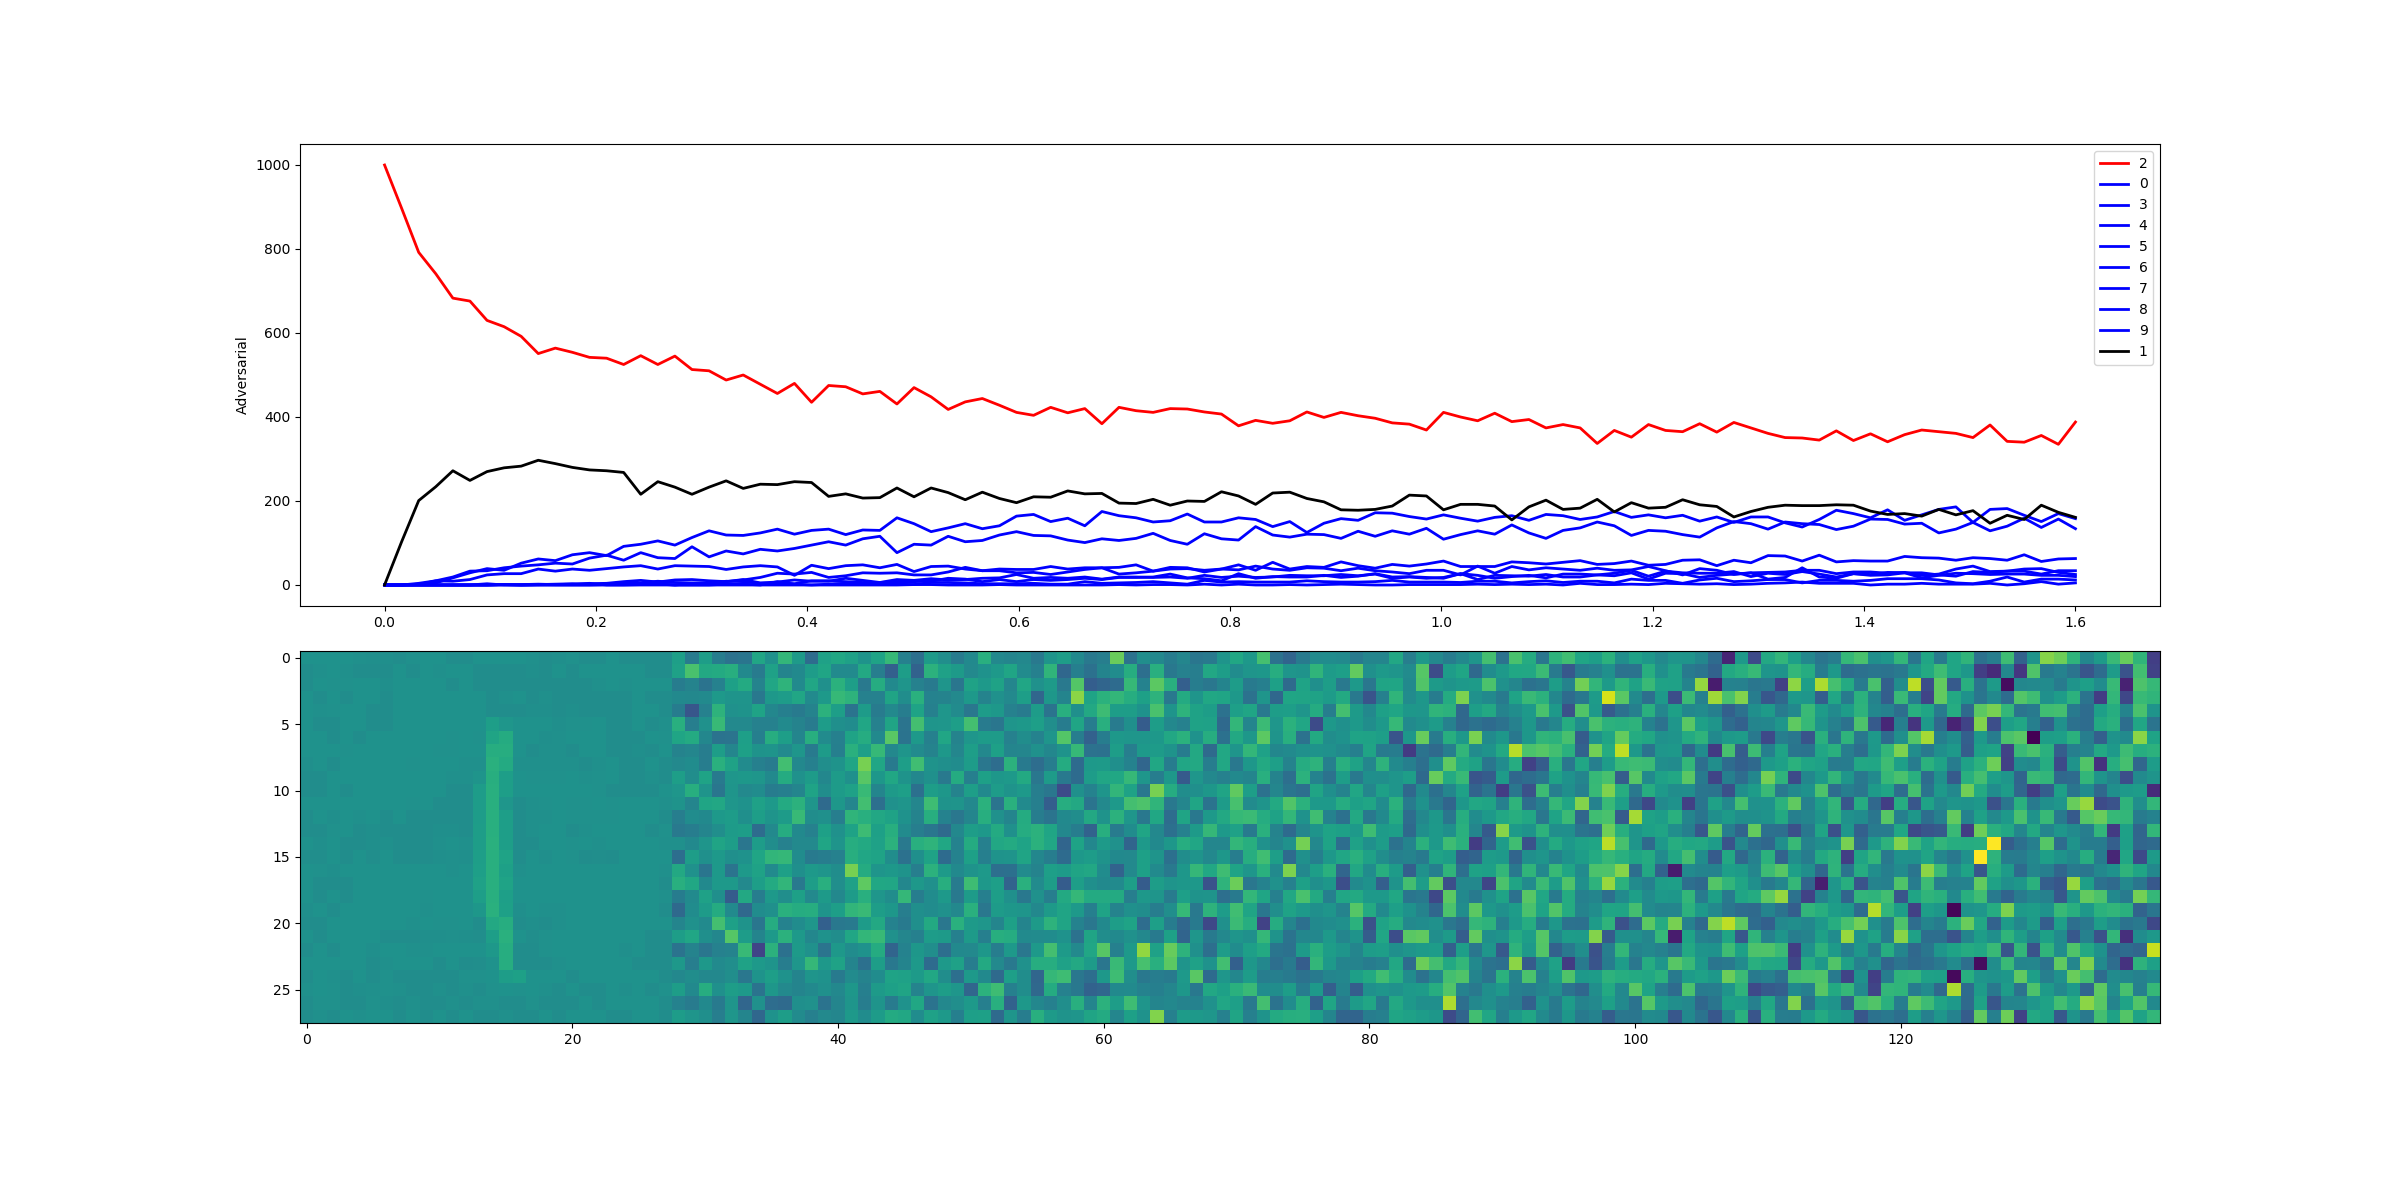
\includegraphics[trim=200 80 100 100, clip,width=7cm]{c2_figures/Image918-O1A2_varx40.png}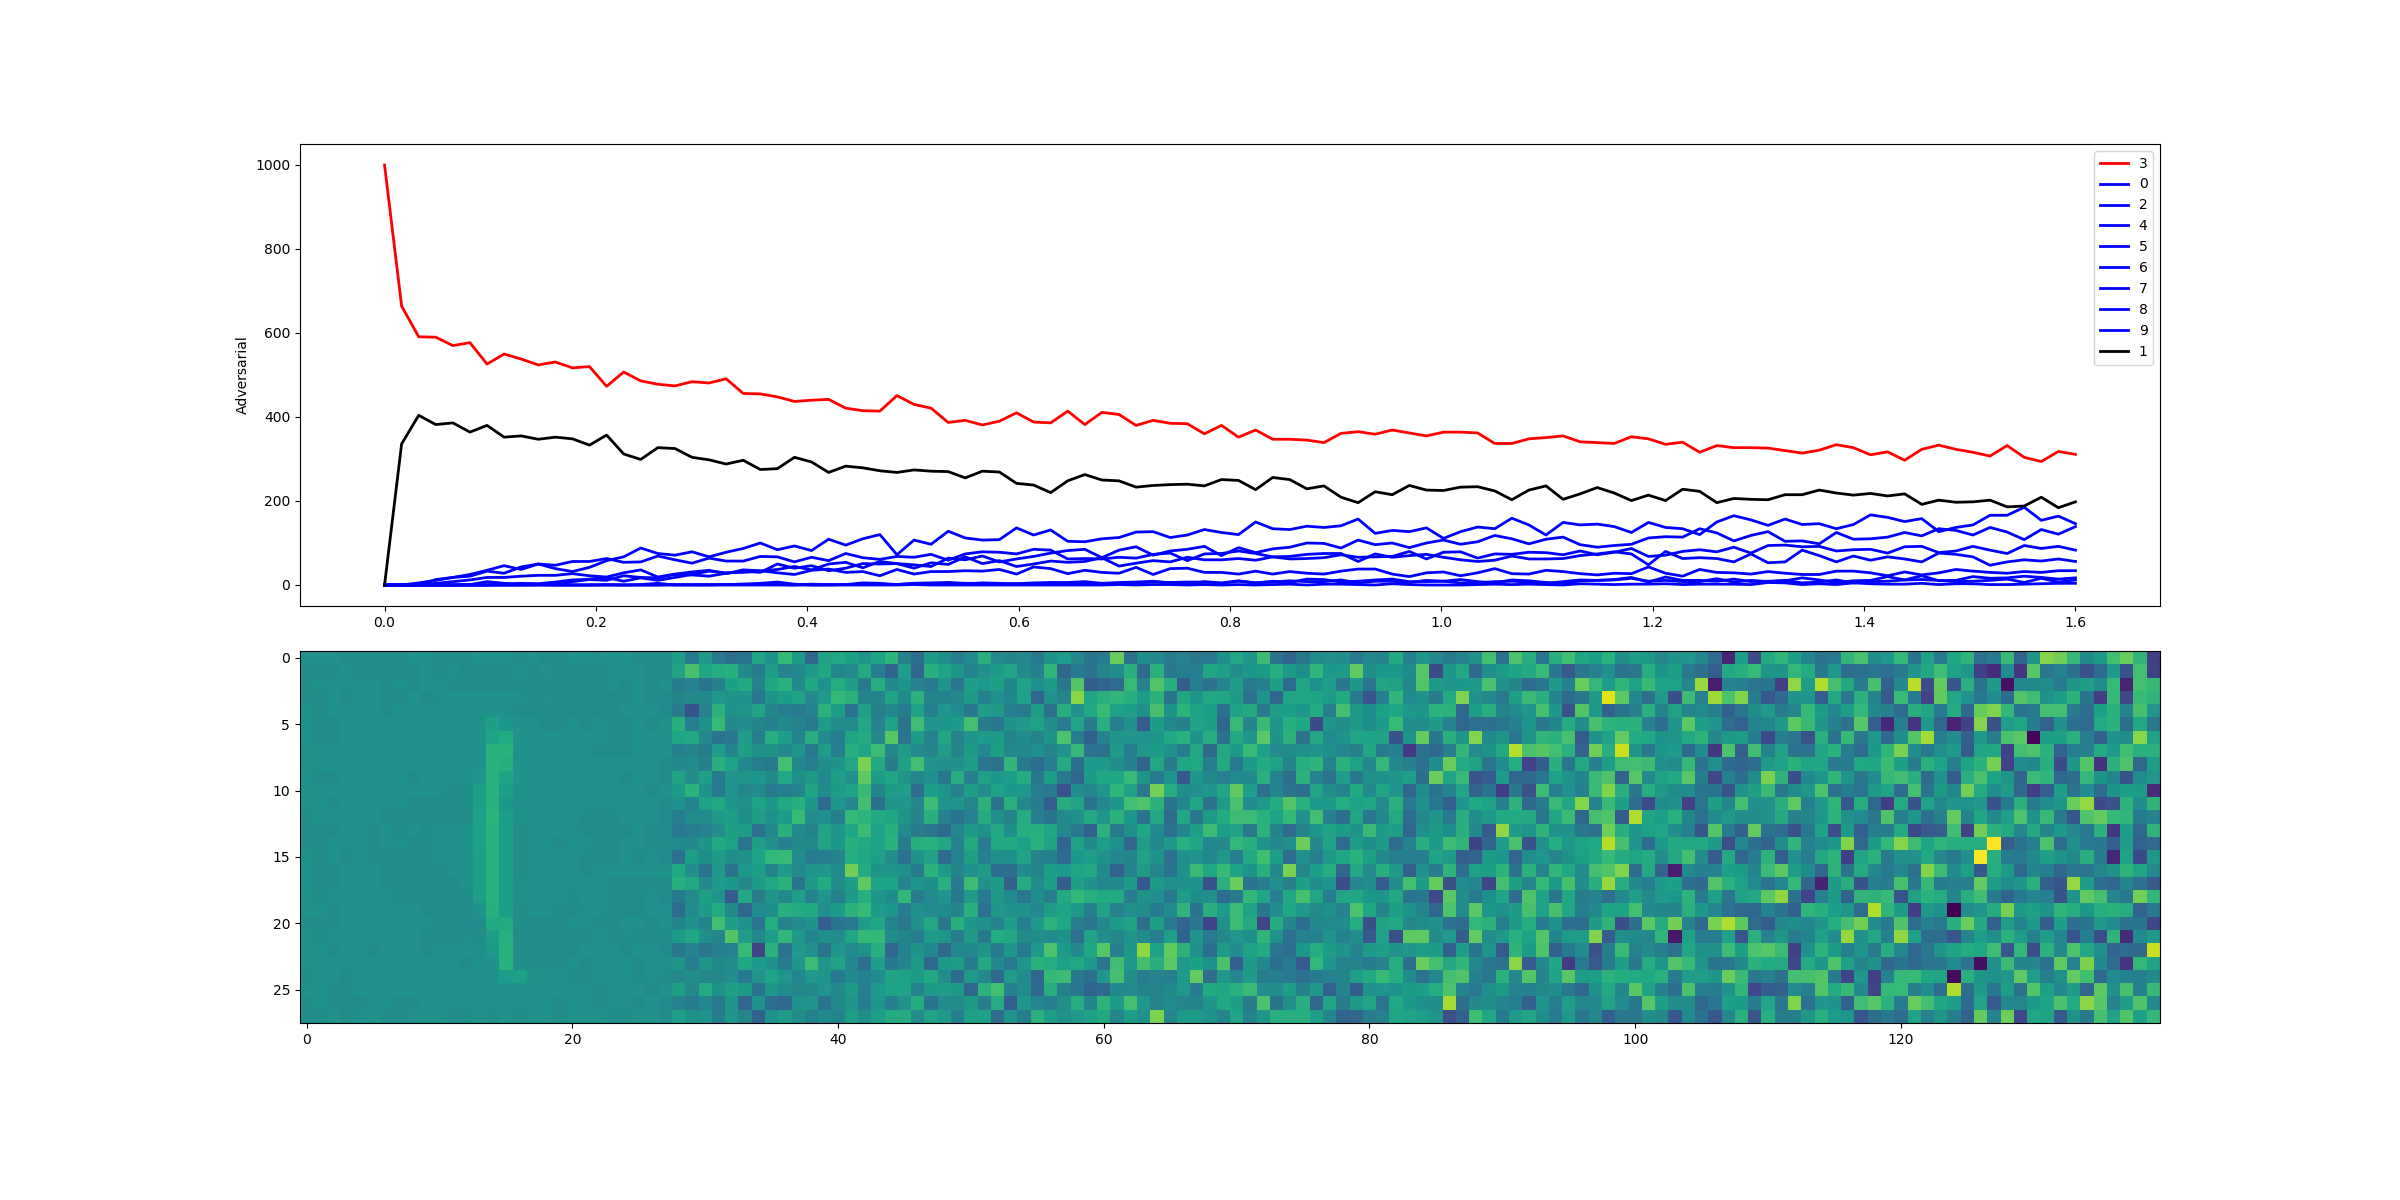
\includegraphics[trim=200 80 100 100, clip,width=7cm]{c2_figures/Image918-O1A3_varx40.png}
% 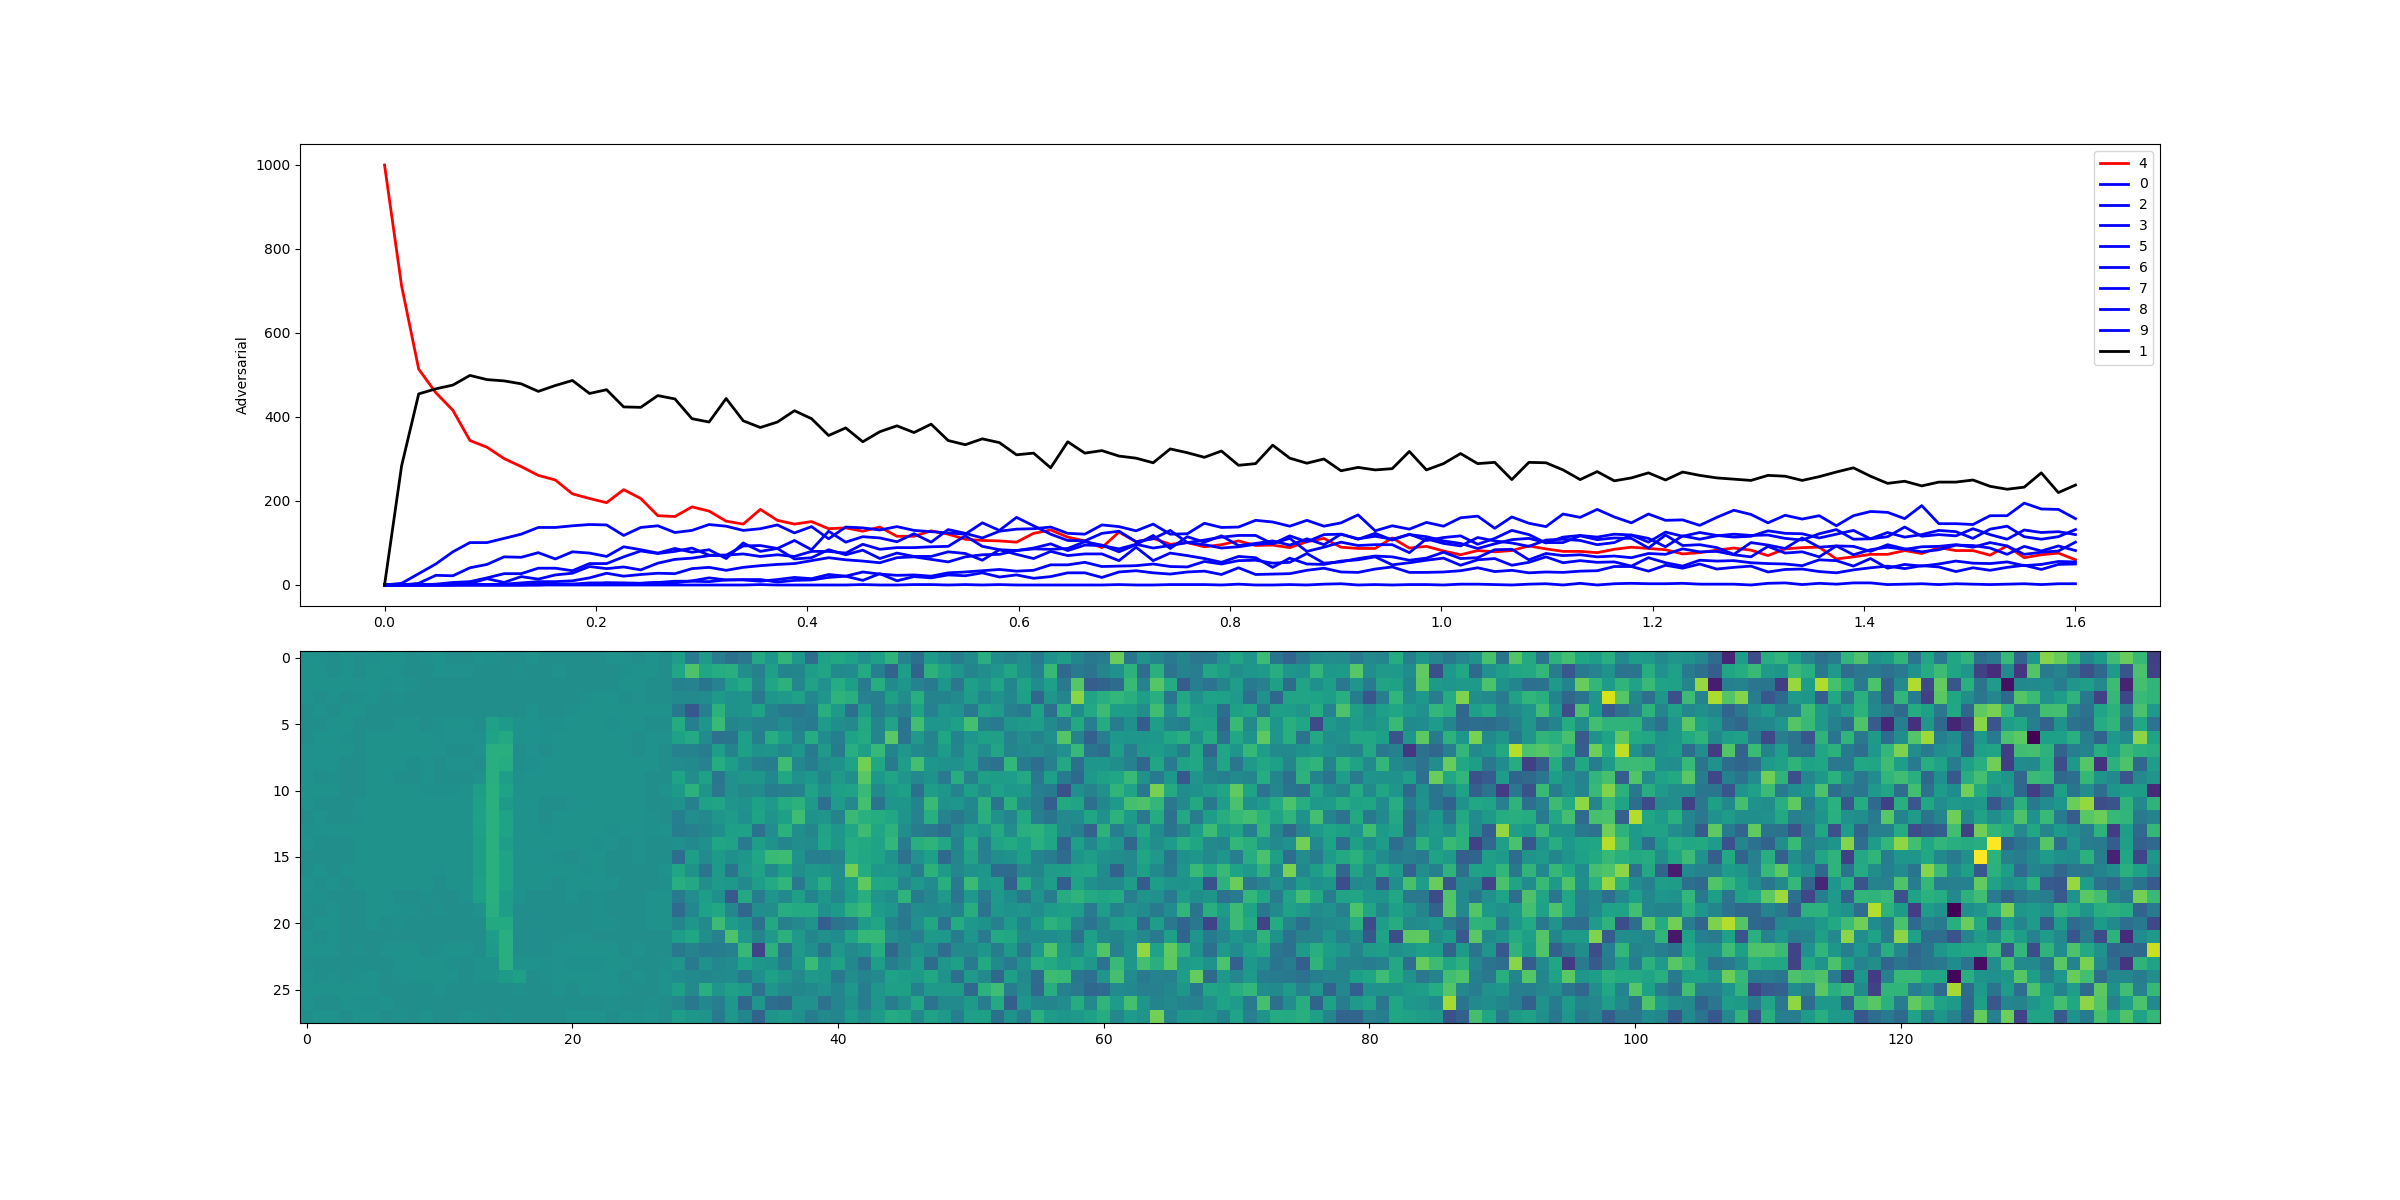
\includegraphics[trim=200 80 100 100, clip,width=7cm]{c2_figures/Image918-O1A4_varx40.png}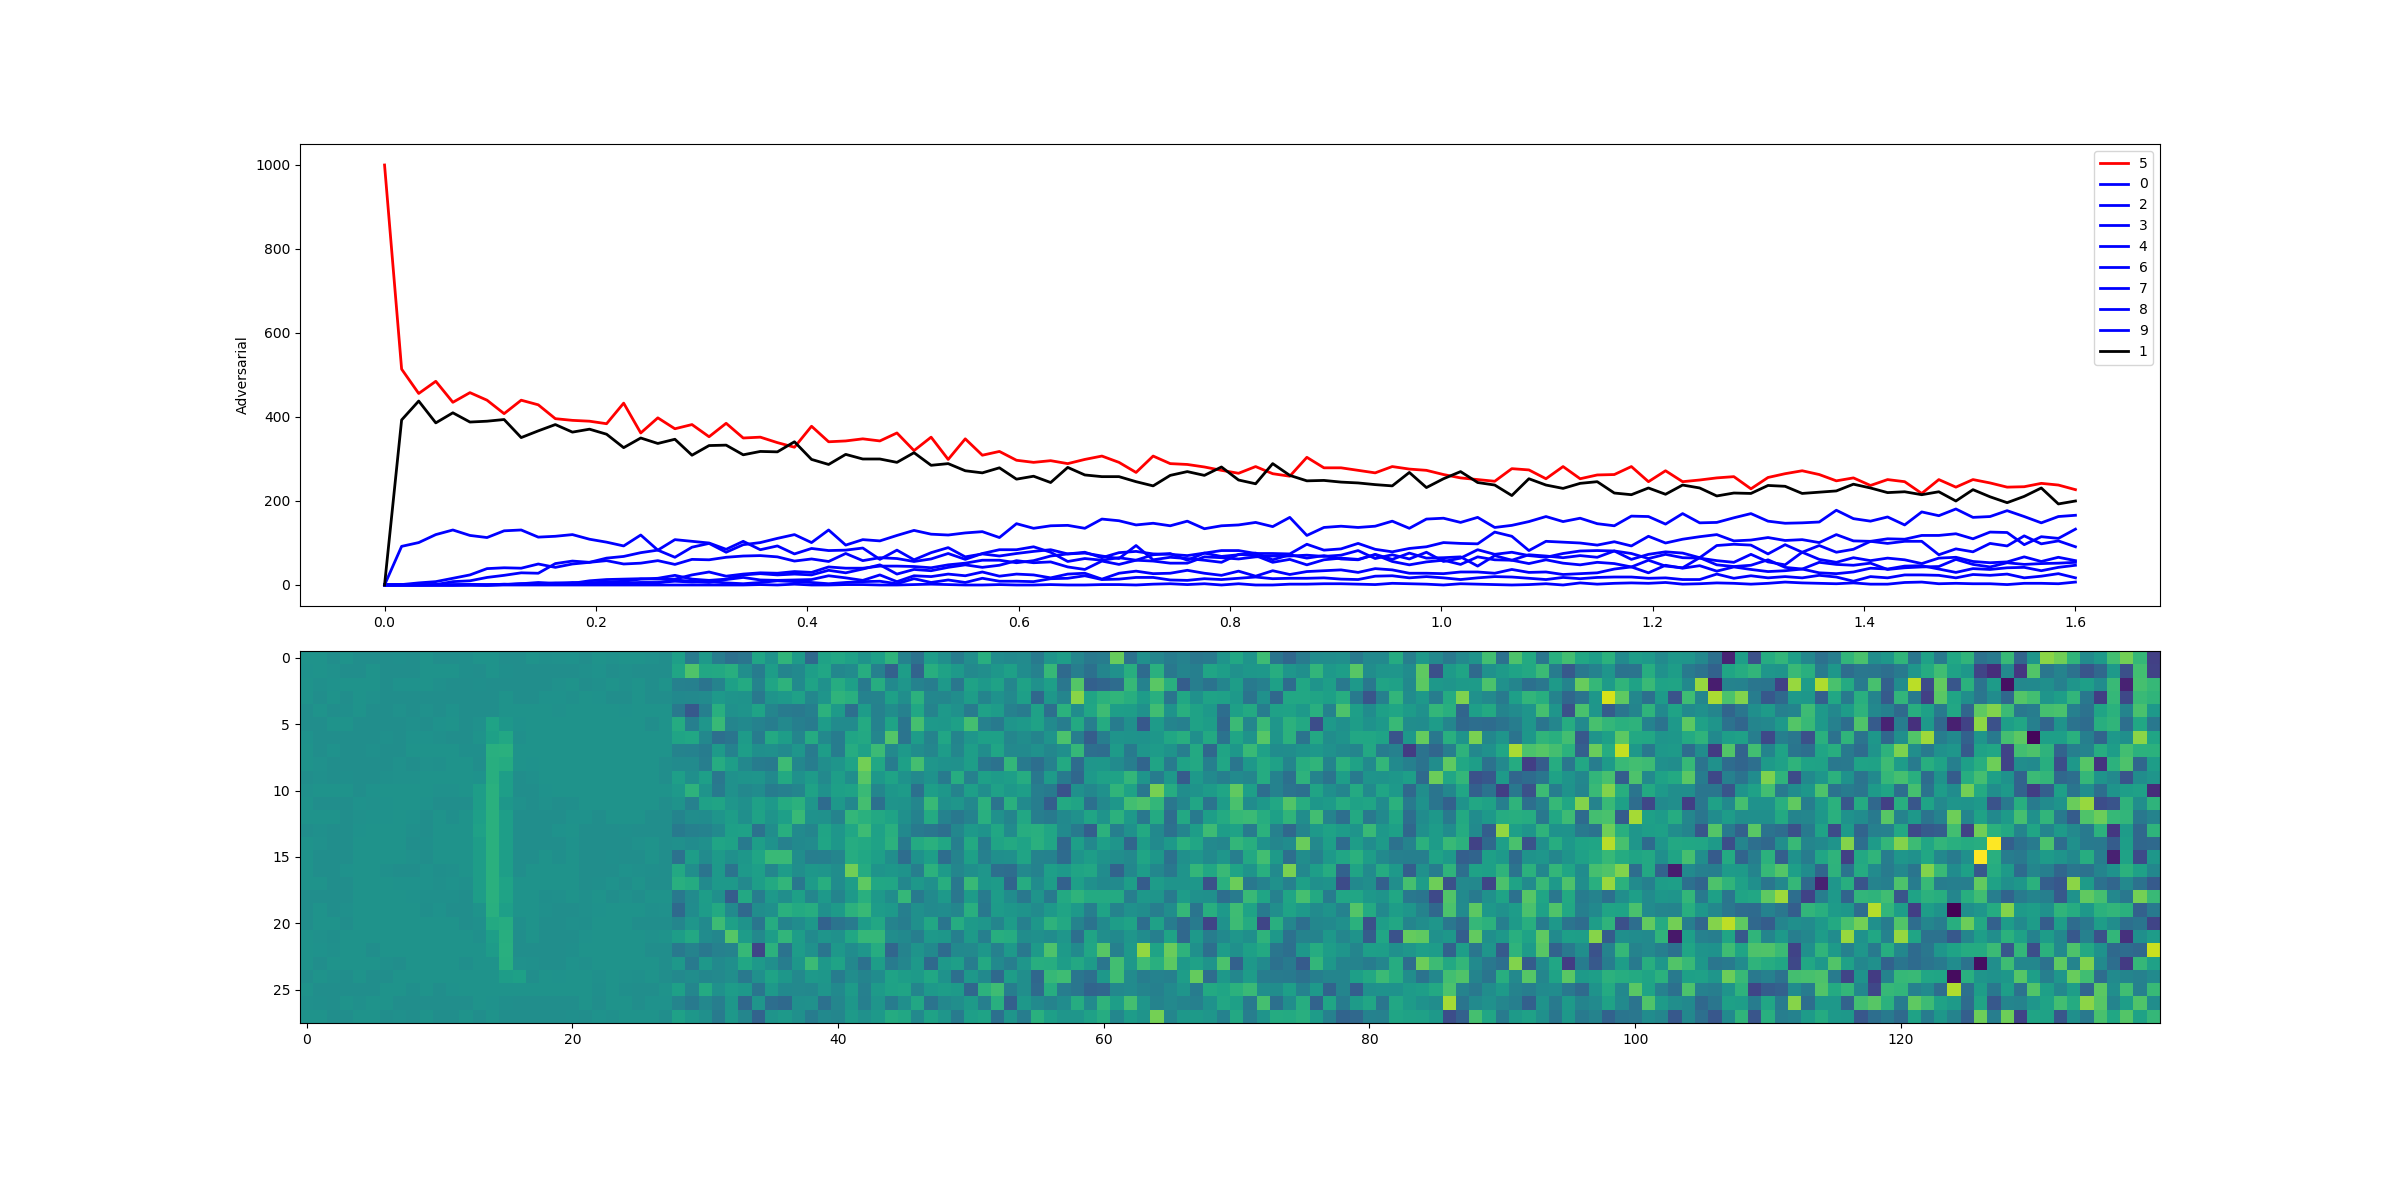
\includegraphics[trim=200 80 100 100, clip,width=7cm]{c2_figures/Image918-O1A5_varx40.png}
% \caption{Frequency of each class in {\it natural} samples with increasing variance around adversarial examples to a $1$ targeted to $2$ (top left), $3$ (top right), $4$ (bottom left), and $5$ (bottom right). The adversarial examples were generated using IGSM. Original Class is shown as a black curve, adversarial in red, all others are blue. 
% Bottom shows example sample images. }
% \label{fgsme}
% \end{figure}

% \begin{figure}[p]
% 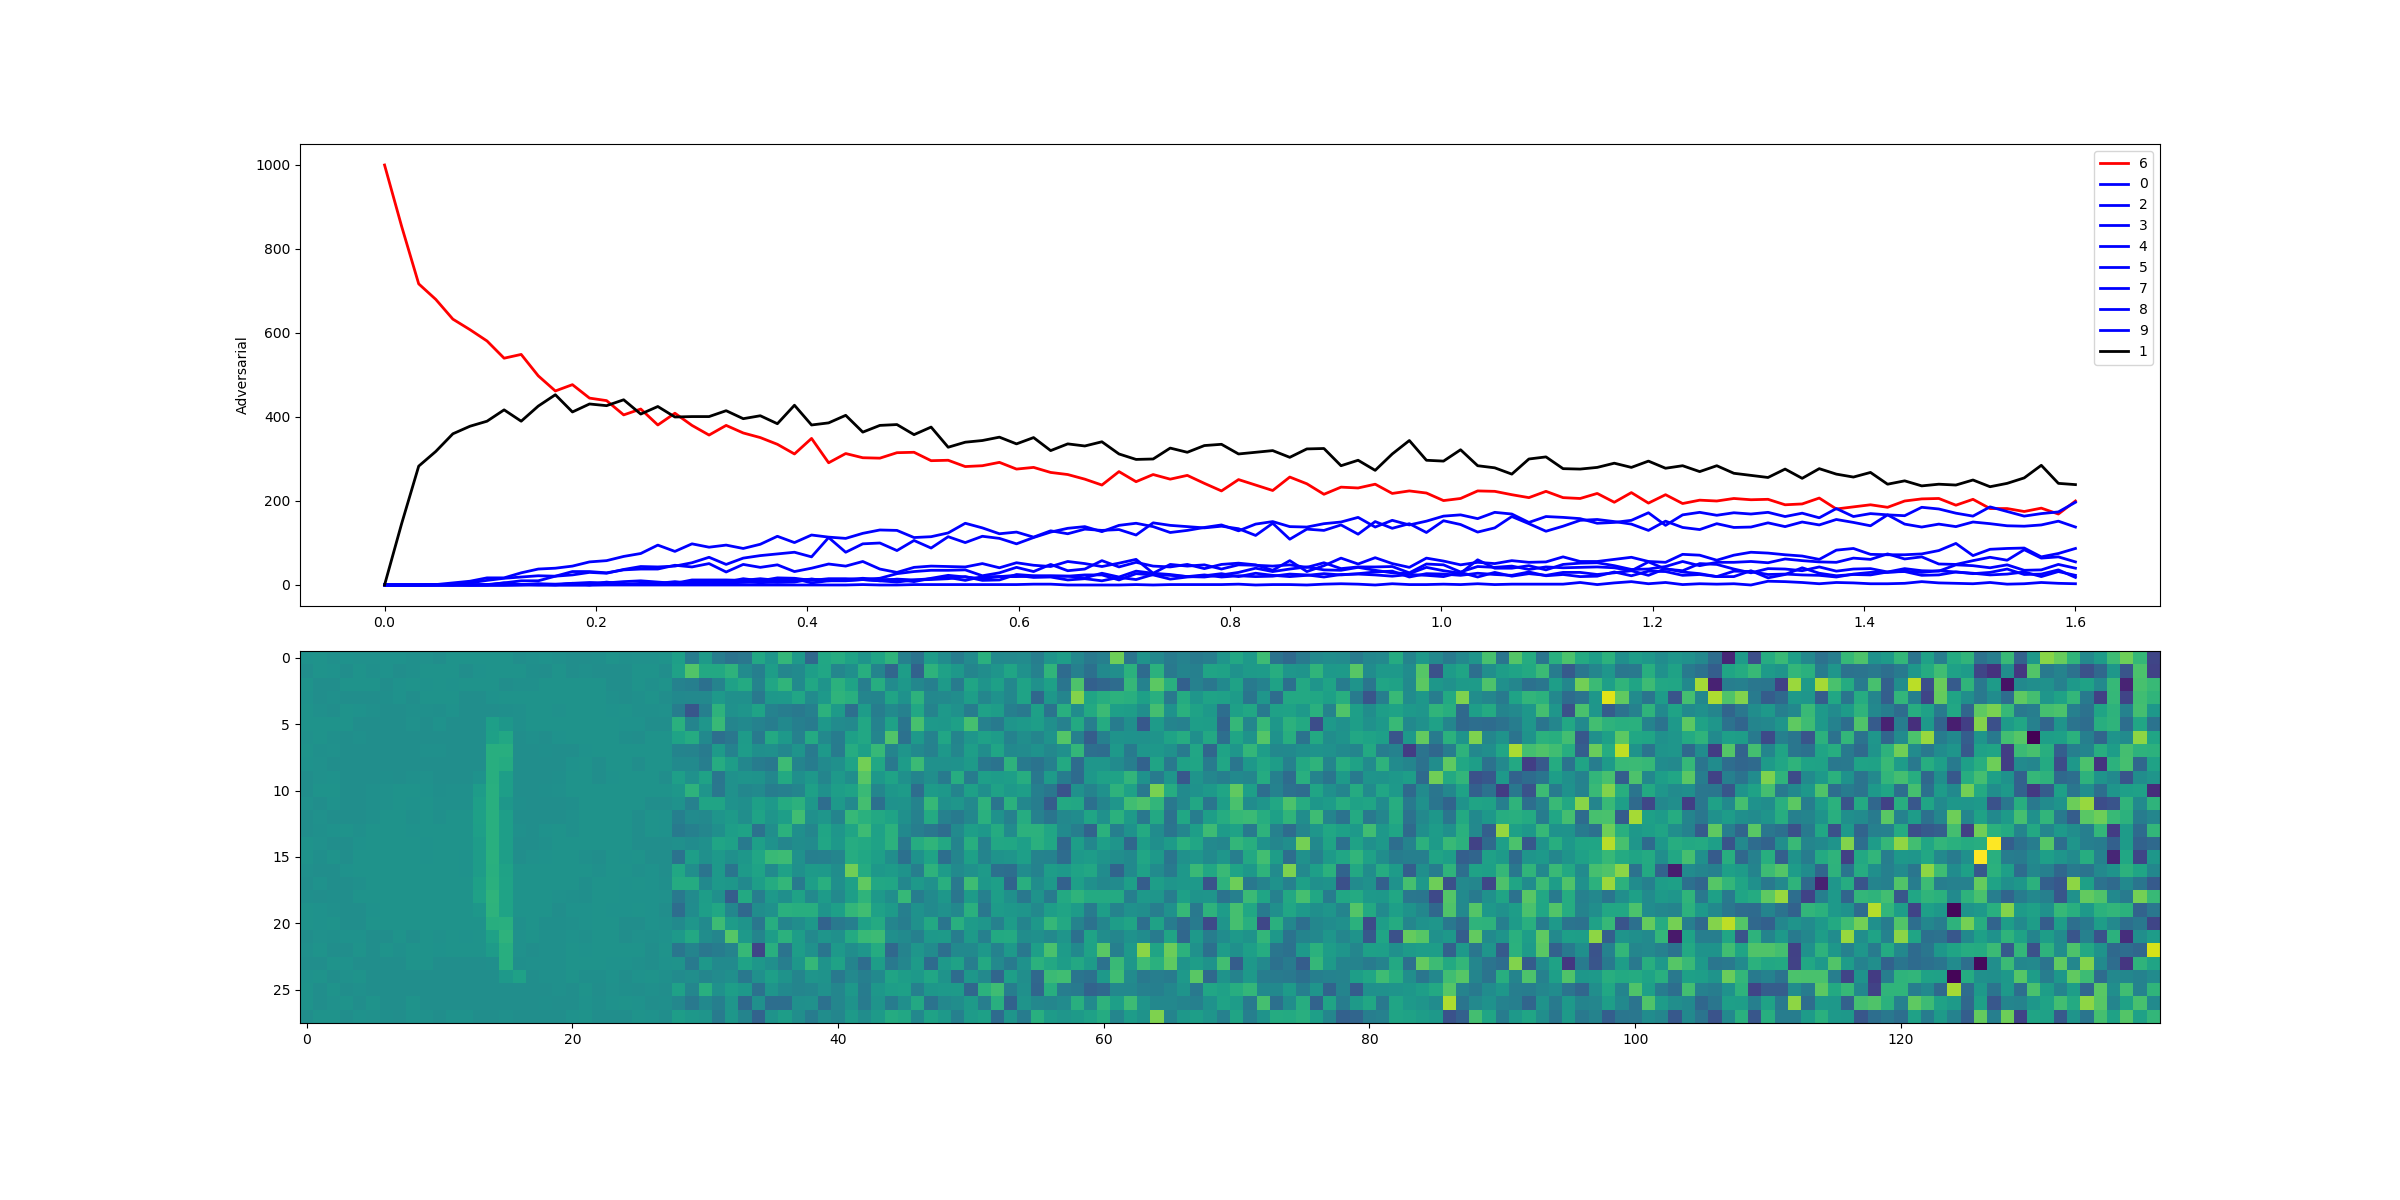
\includegraphics[trim=200 80 100 100, clip,width=7cm]{c2_figures/Image918-O1A6_varx40.png}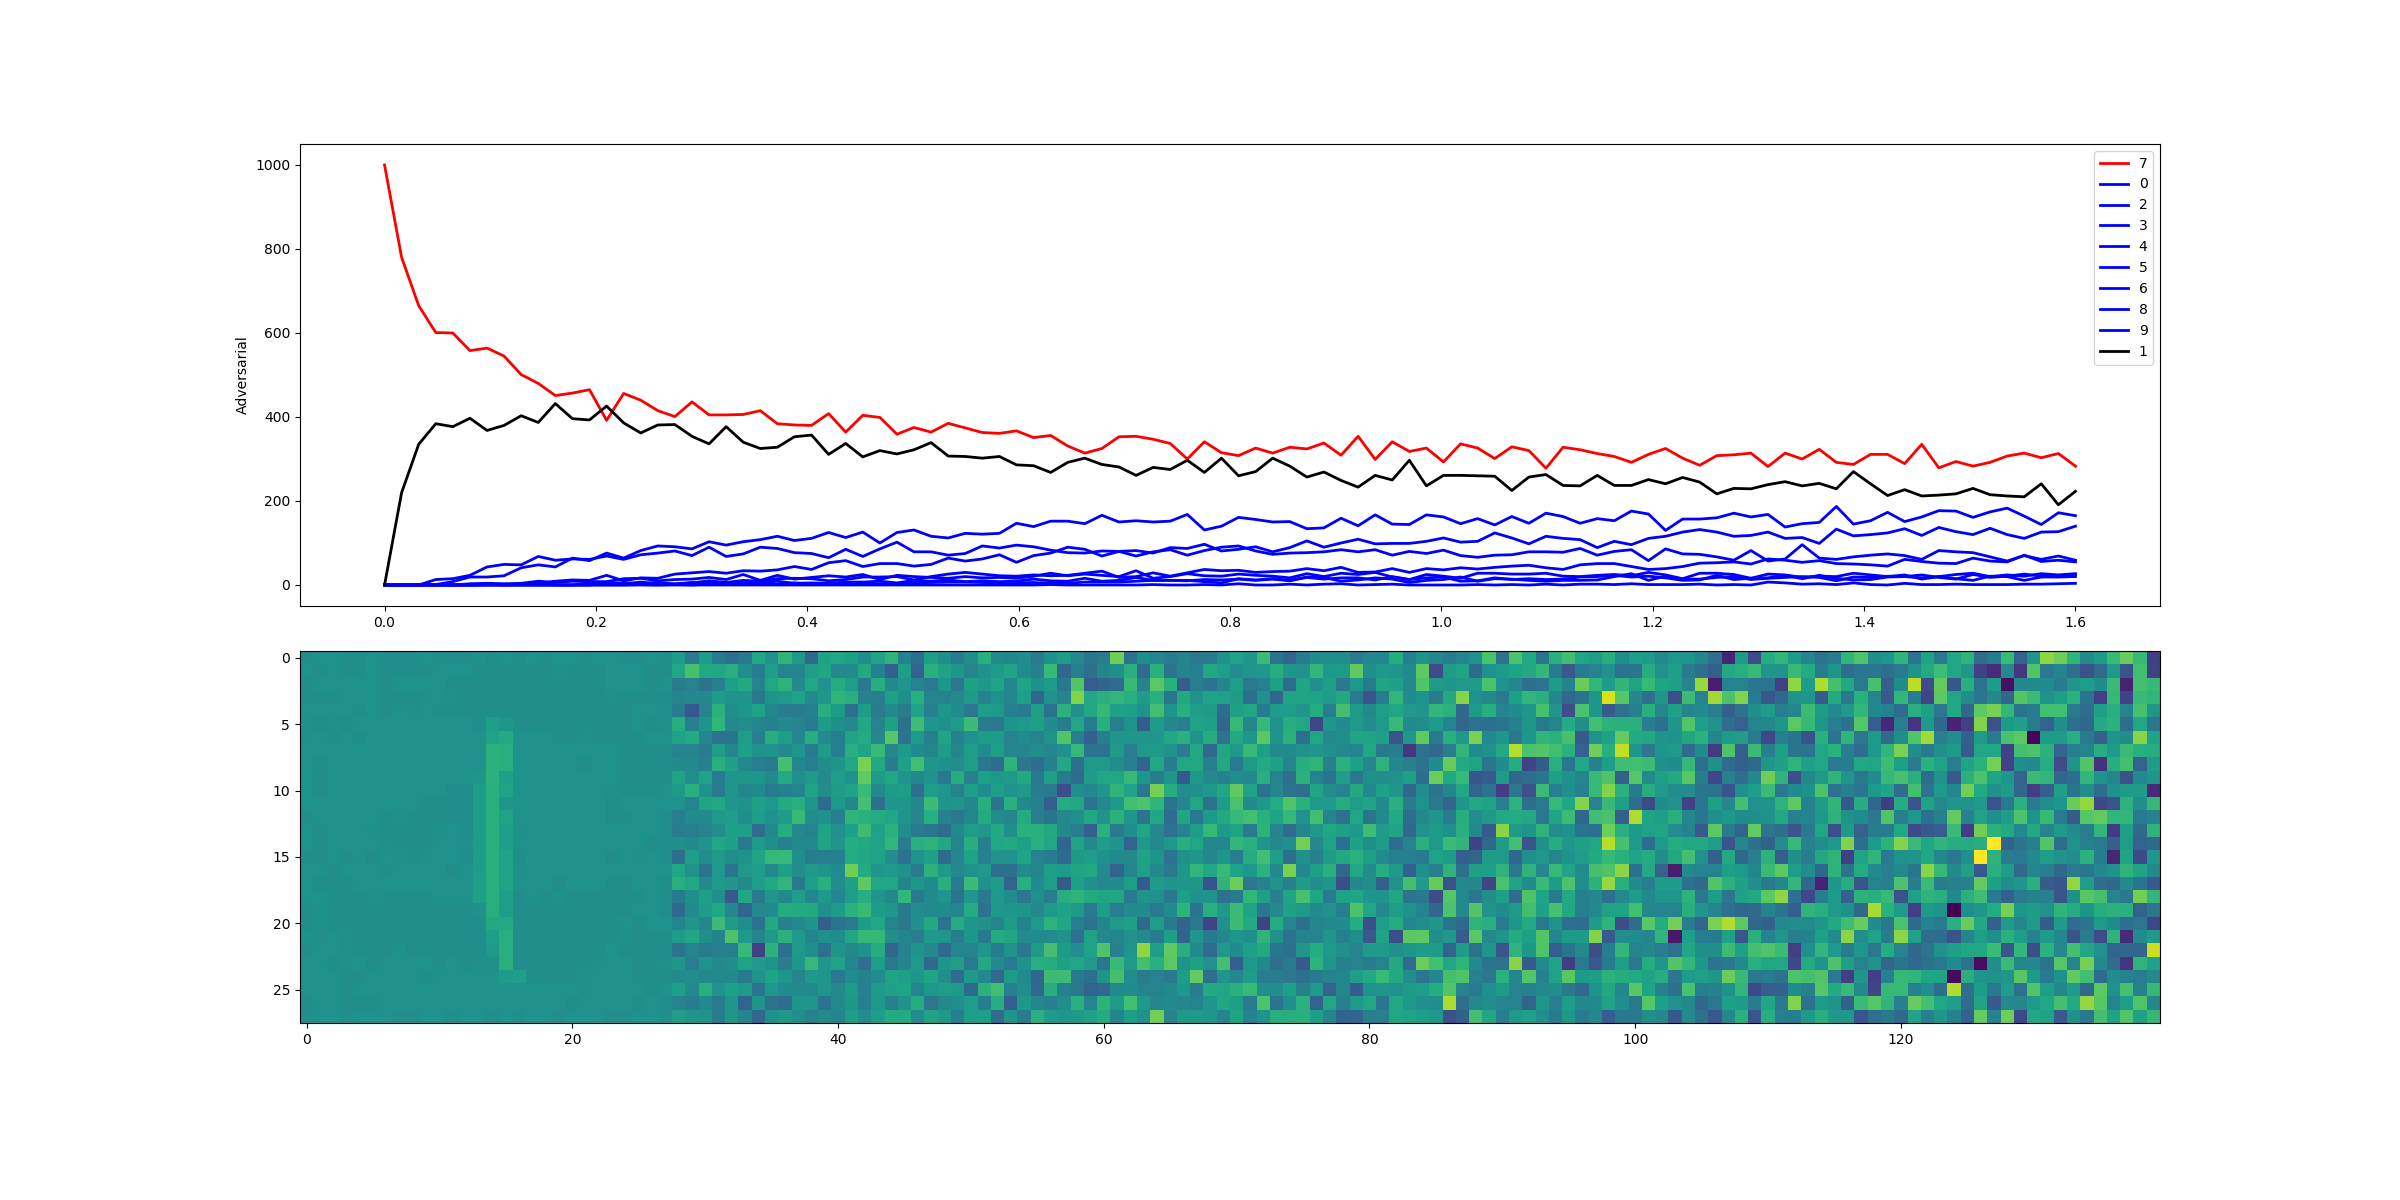
\includegraphics[trim=200 80 100 100, clip,width=7cm]{c2_figures/Image918-O1A7_varx40.png}
% 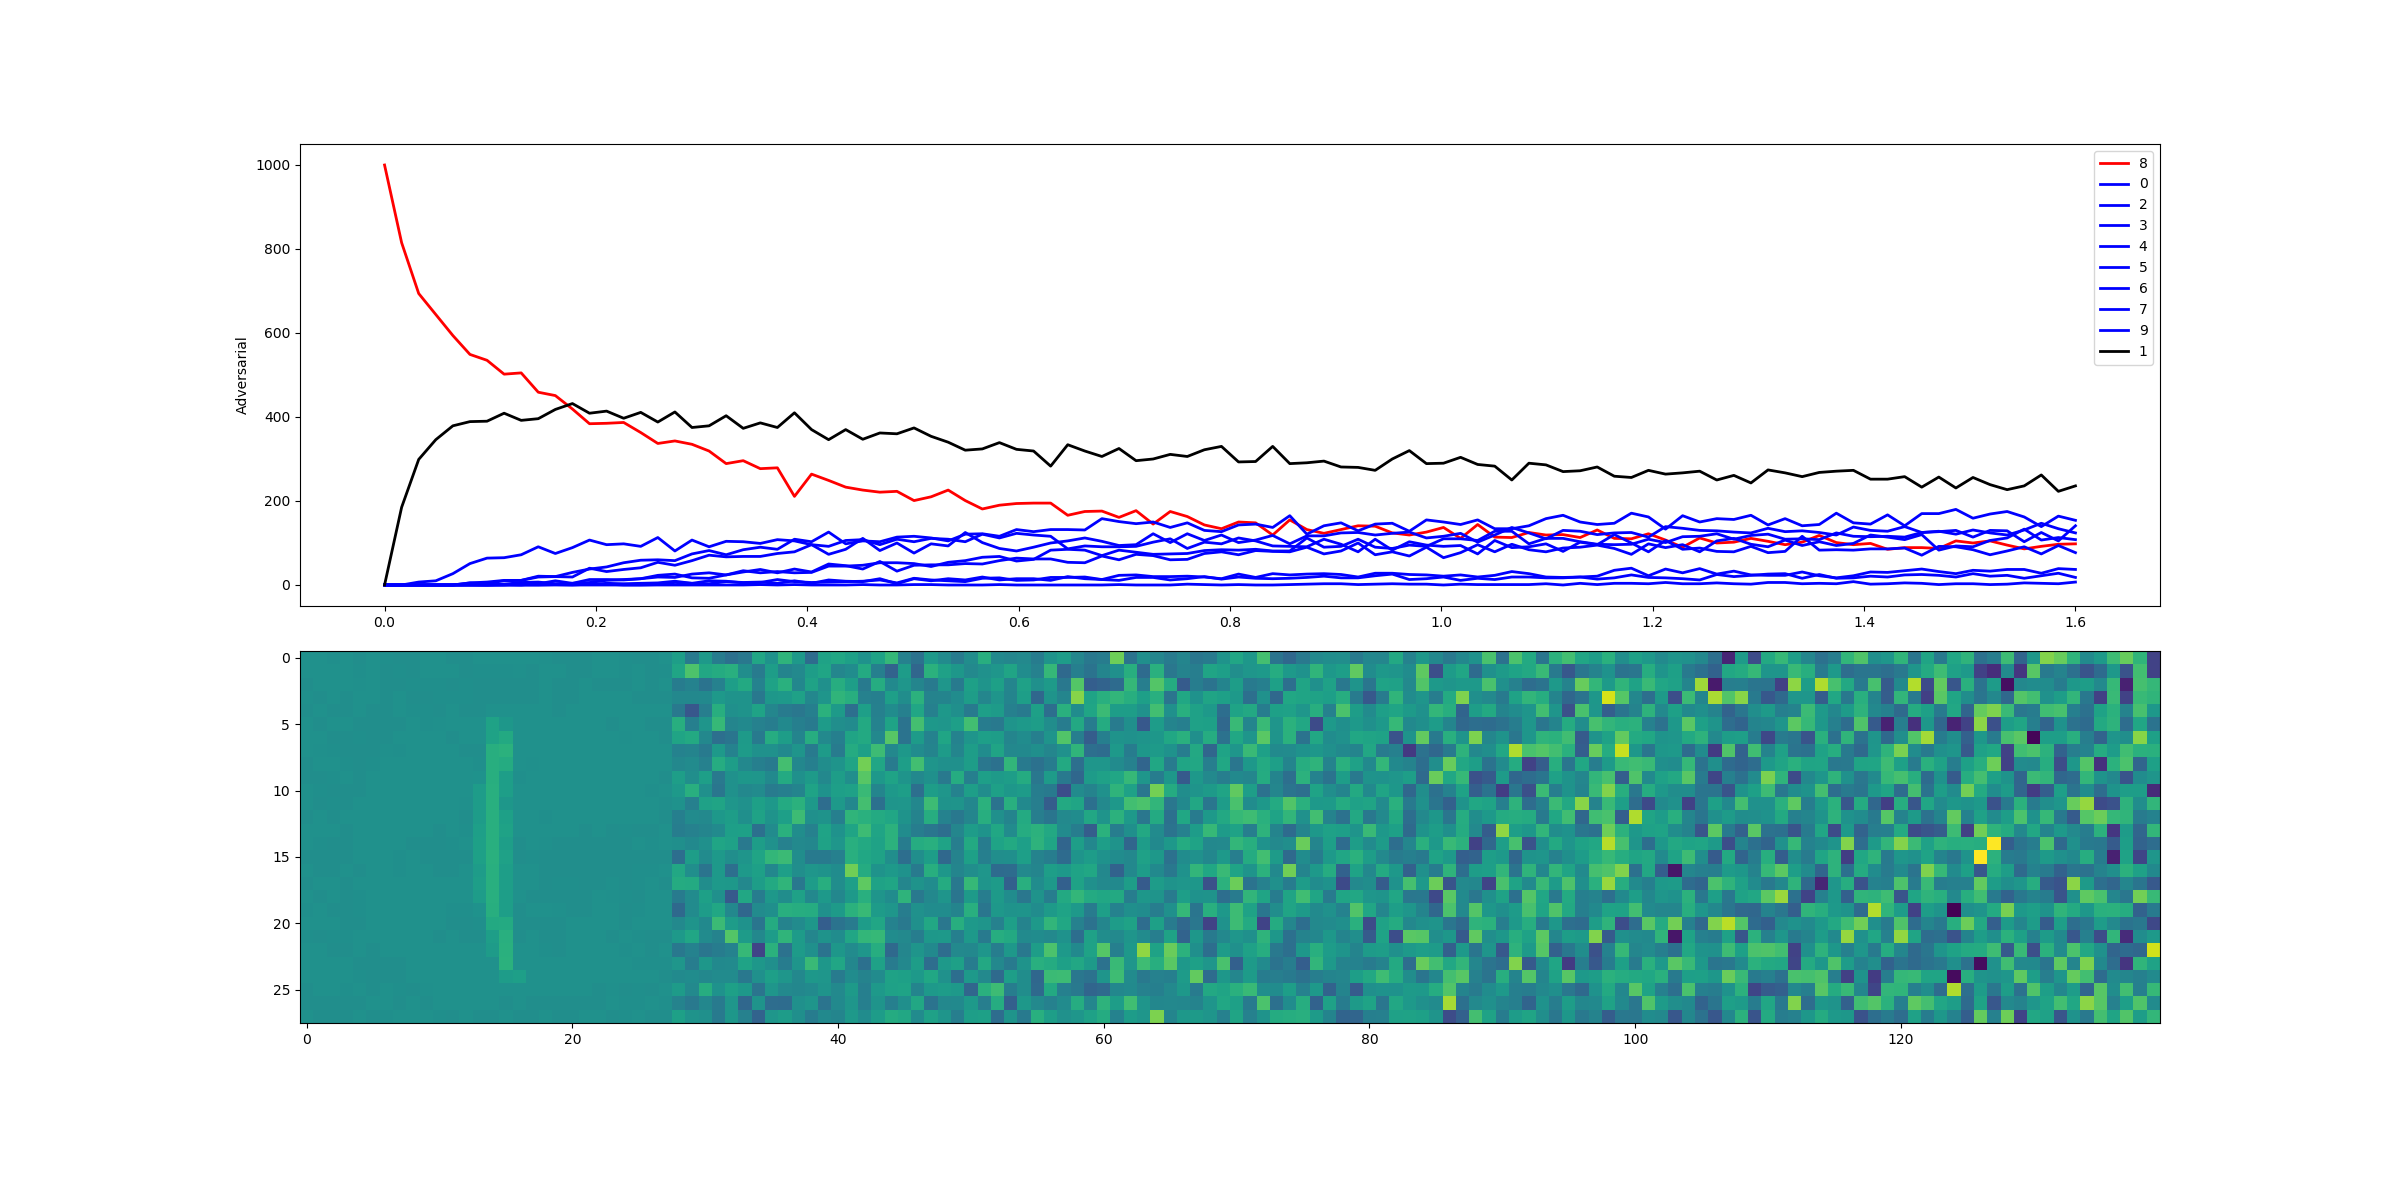
\includegraphics[trim=200 80 100 100, clip,width=7cm]{c2_figures/Image918-O1A8_varx40.png}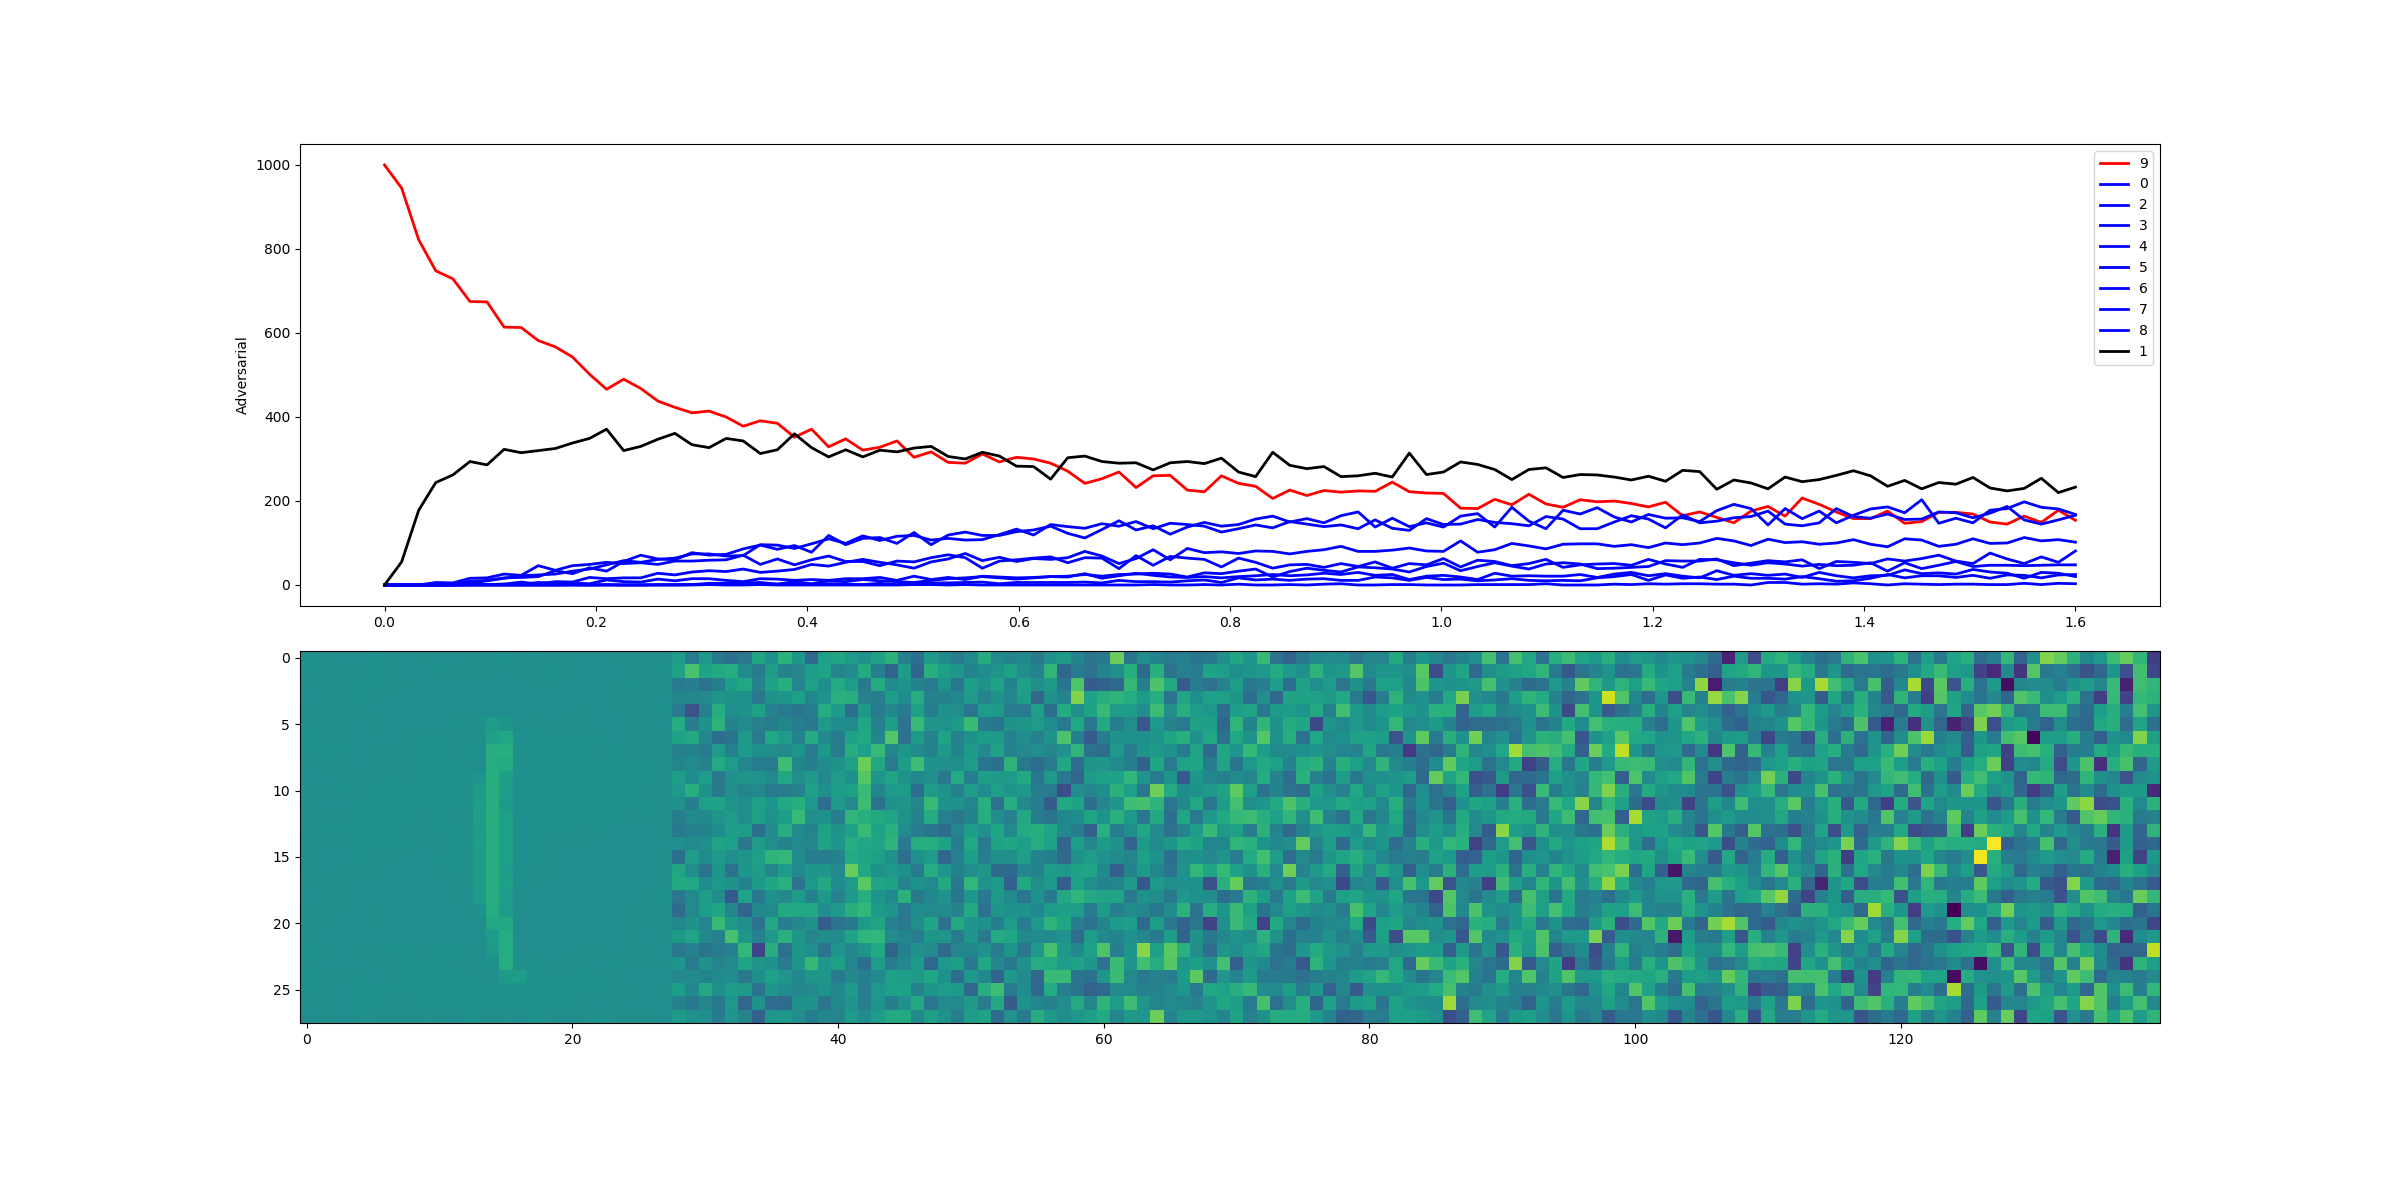
\includegraphics[trim=200 80 100 100, clip,width=7cm]{c2_figures/Image918-O1A9_varx40.png}
% \caption{Frequency of each class in {\it natural} samples with increasing variance around adversarial examples to a $1$ targeted to $6$ (top left), $7$ (top right), $8$ (bottom left), and $9$ (bottom right). The adversarial examples were generated using IGSM. The original class is shown as a black curve, adversarial in red, all others are blue. Bottom shows example sample images. }
% \label{fgsmh}
% \end{figure}


% The neighborhoods around datapoints and adversarial examples are sampled using Gaussians with varying standard deviation $\sigma$, and Algorithm \ref{bracketing} is used to approximate $\gamma$-persistence corresponding to $\gamma=0.7$. The resultant $0.7$-persistence $\sigma$ statistically identifies examples as being $(0.7,\sigma)$-stable, meaning that 70\% of the samples drawn from a Gaussian with standard deviation $\sigma$ are classified the same as the original class by the model. 

% We will consider adversarial examples in the context of two widely used datasets, MNIST digits \cite{MNIST} and ImageNet \cite{Imagenet}.

% % \subsubsection{Gamma-Sigma Stability of FGSM attacks on MNIST}

% % In these initial experiments, the neighborhood around normal and adversarial examples are analyzed via sampling. An image $x$ with classification $\ell$ is selected, adversarial noise $x_a$ is prepared 

% % \begin{figure}[t]
% %   \centering
% % 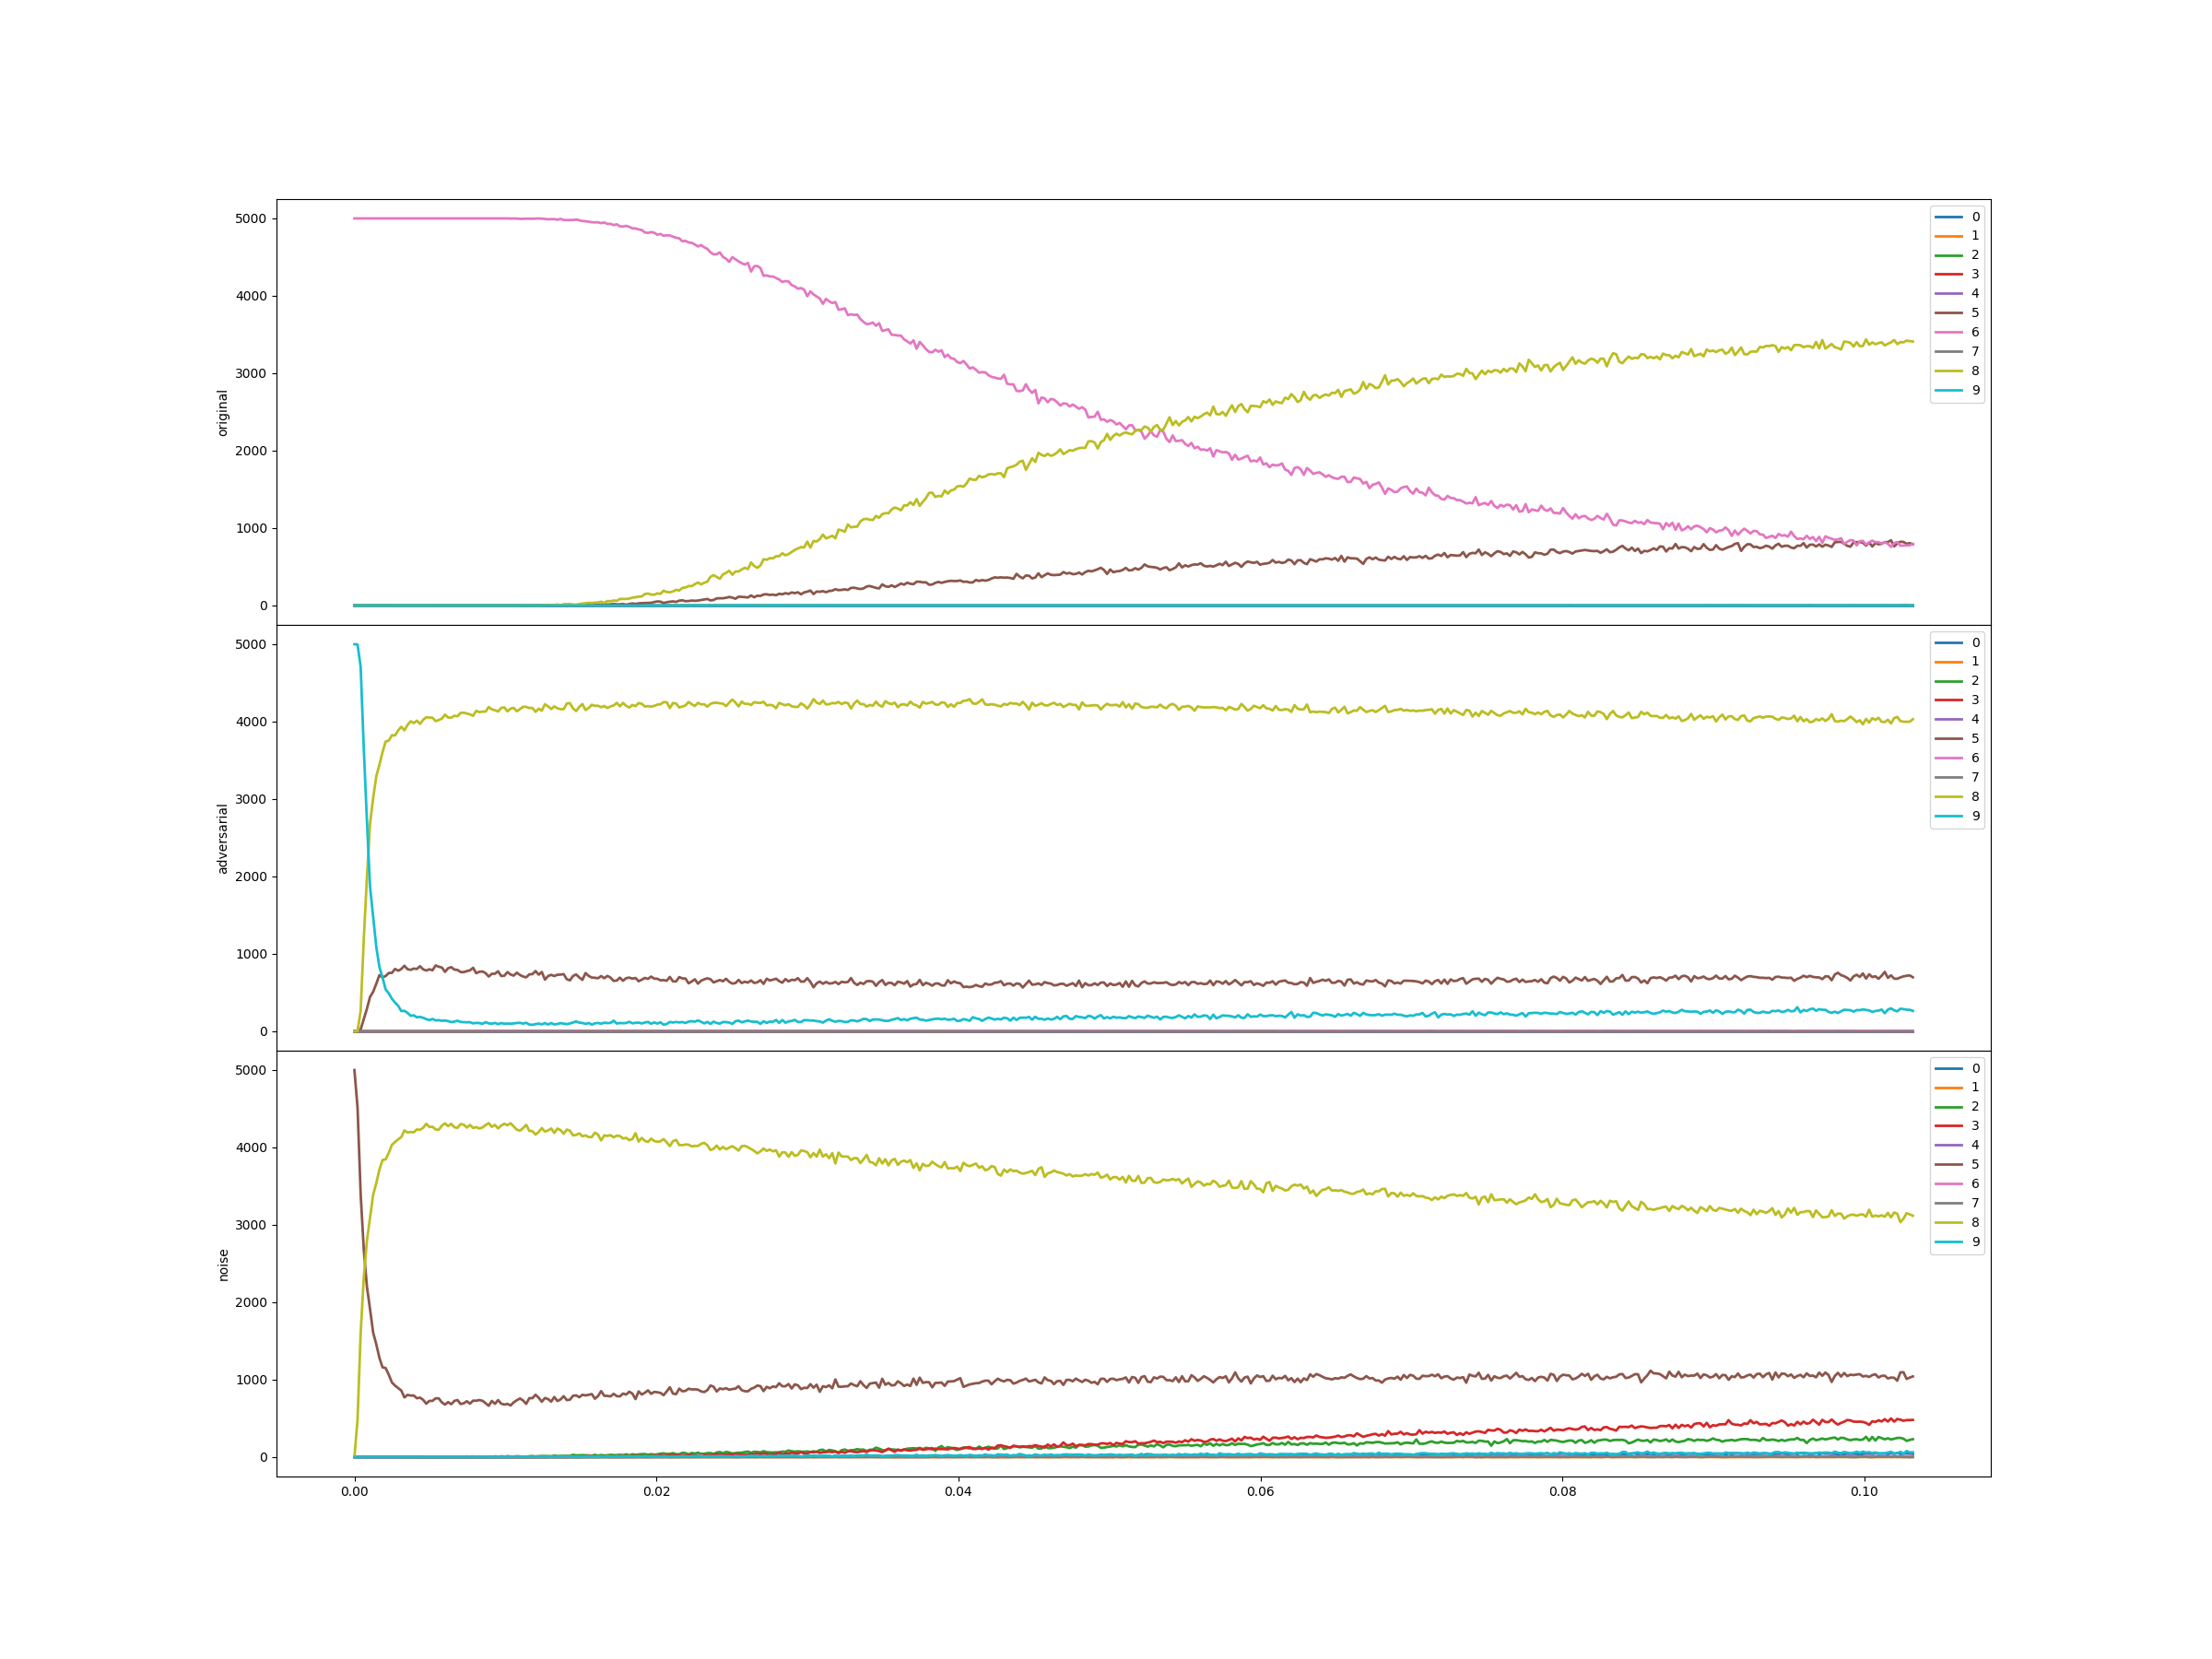
\includegraphics[width=11cm]{c2_figures/O6A9_varx40.png}
% % 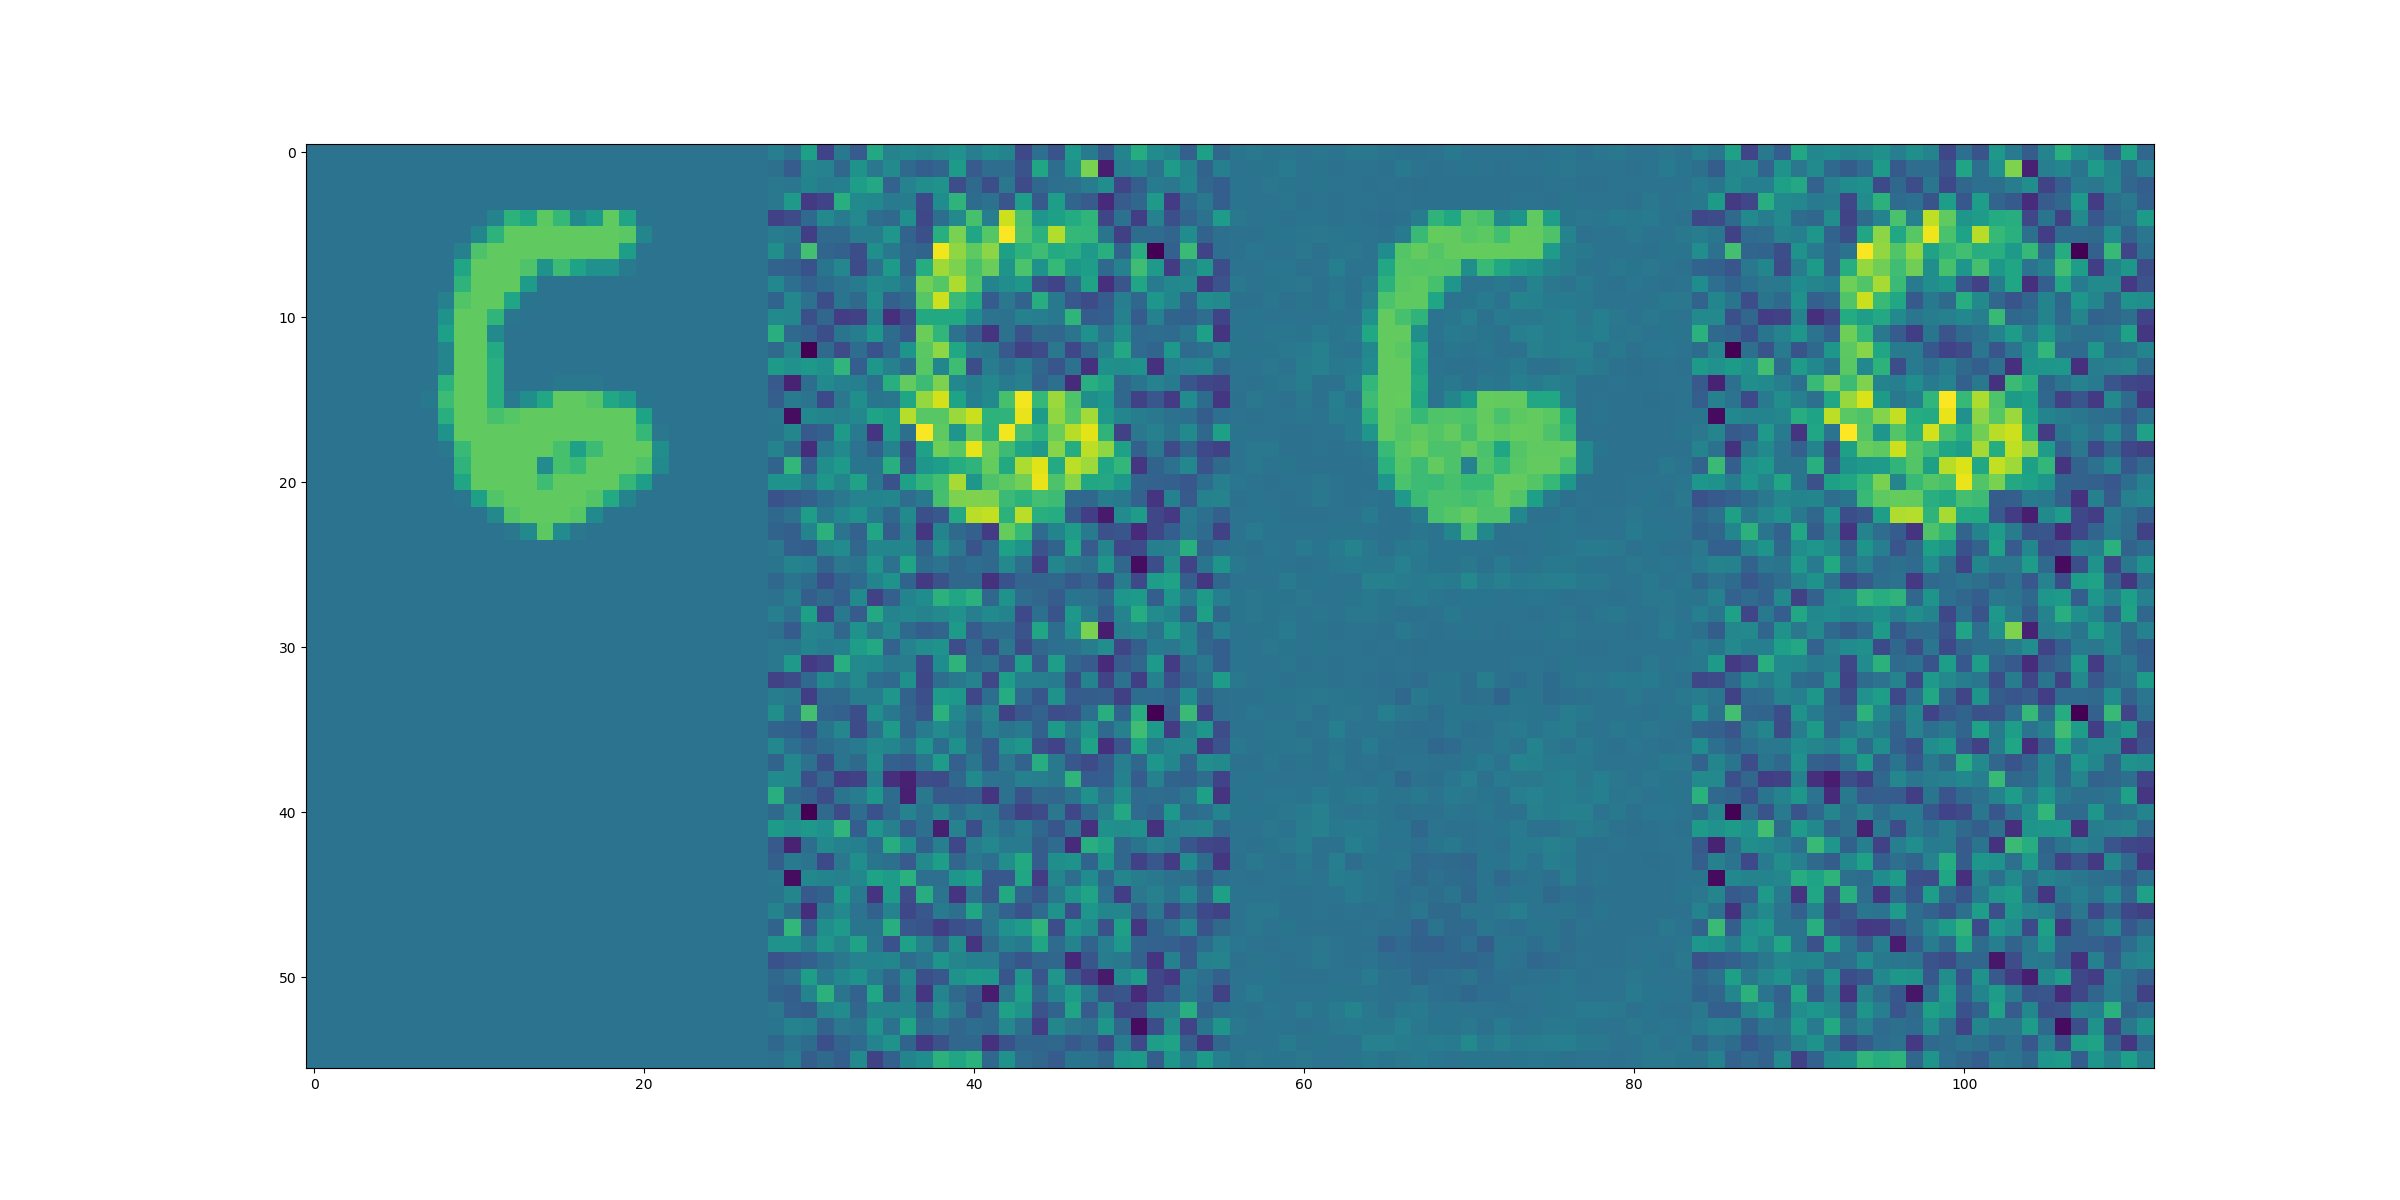
\includegraphics[width=11cm]{c2_figures/O6A9_varx40_examp.png}
% %   \caption{Top image shows how a regular image, an adversarial image,
% %     and plain noise get classified with added noise indicated on the
% %     $x$-axis. Second image shows in order the Original, IID Gaussian
% %     noise added,  adversarial noise added, and IID Gausian plus
% %     adversarial noise added. }
% % \end{figure}

% % This sampling approach was Each
% % adversarial image in this dataset was bracketted using the sampling
% % technique described above. Within Class 0 of ImageNet (tench/tinca (A
% % type of fish)), 487 samples were processed and of these, 482 met a 5\%
% % threshold, i.e. were less than 95\% of the bracketed additive noise
% % sample distances. This indicates that in exchange for 5\%
% % classification accuracy, we were able to correctly filter out 99.17\%
% % of the adversarial examples. \\




% \subsubsection{$(\gamma, \sigma)$-stability for adversarial examples on ImageNet}
% [??DG?? This section needs picture similar to the previous section] Similar to the above analysis for MNIST, an image $x$ was selected with original class "Rose-Hip," and then an perturbation $x_a$ was found using IGSM so that the sum $x + x_a$ is an adversarial example with class "Baseball." Then 50 Gaussian samples were generated for each of 1000 evenly spaced standard deviation $\sigma$ values. These samples were added to $x$ and $x+x_a$. Figure  \ref{fig:IGSMpersistenceImageNet} shows classifications are colored via a heatmap.

% \begin{figure}[p]
% 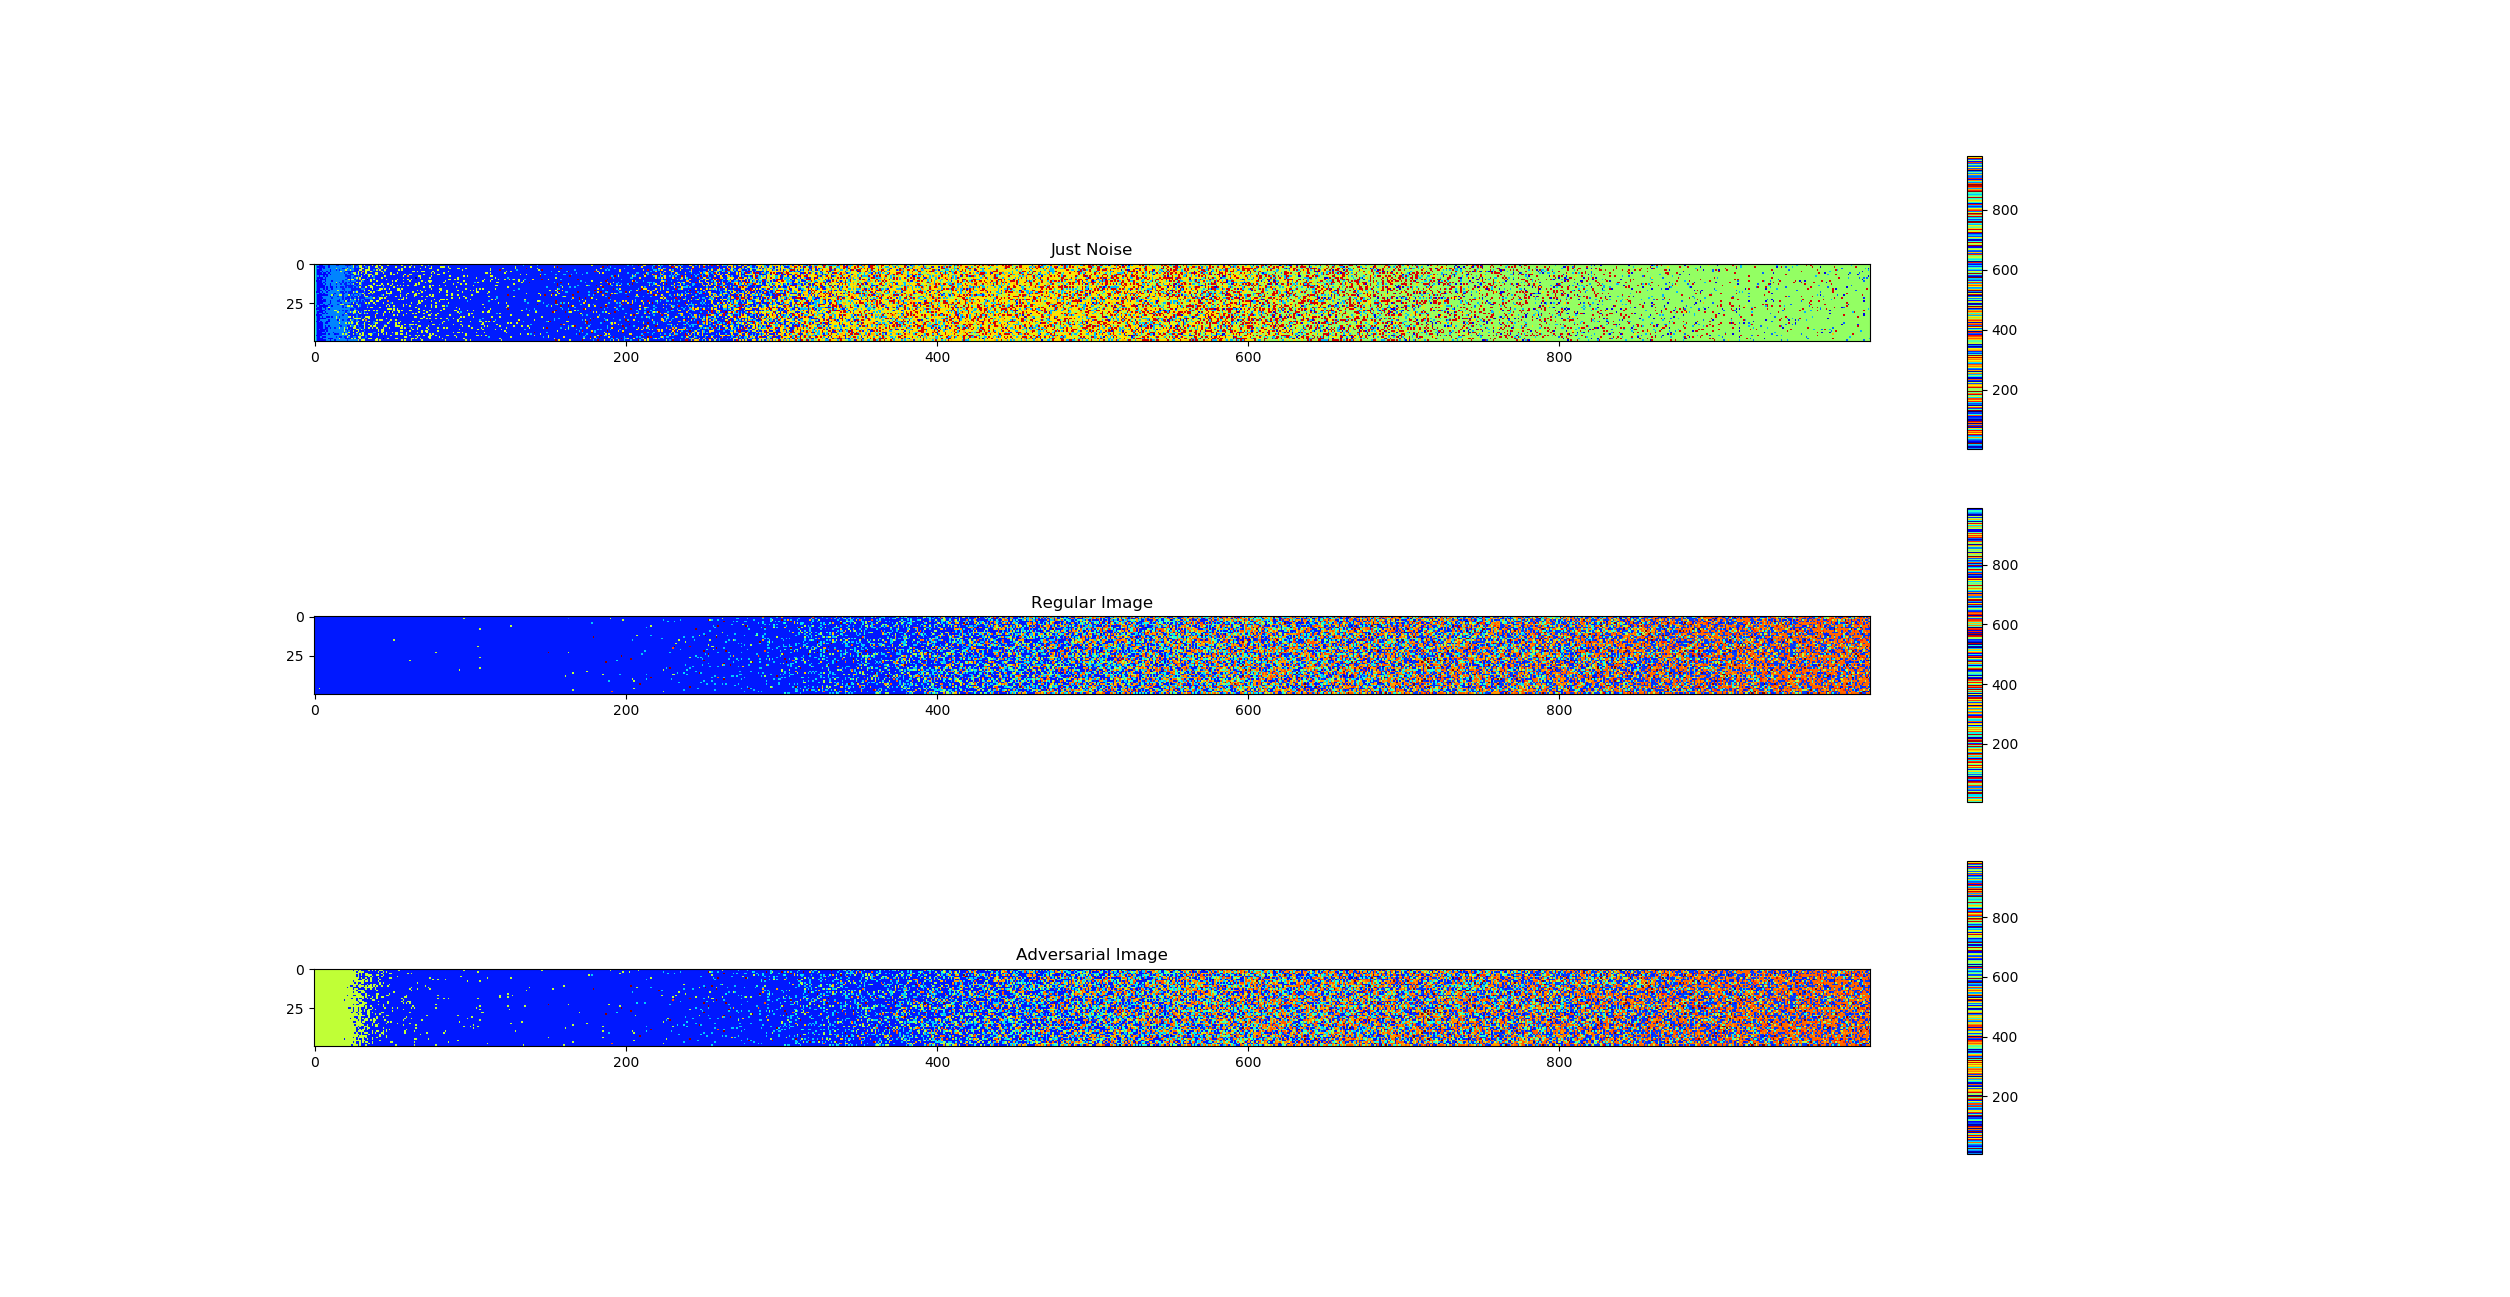
\includegraphics[width=14cm]{c2_figures/50r1000x_cmap_rand.png}
% \caption{??DG: This is not readable. Heatmaps indicating frequency in each class??? when Gaussian samples are added with given $\sigma$ values. Top starts with a pure black image,
% middle starts with $x$ (the original image), and
% bottom starts with $x + x_a$ (the adversarial image).}
% \label{fig:IGSMpersistenceImageNet}
% \end{figure}

% The $0.7$-persistence of 50 natural examples (DG: of rose hip?) are shown in Figure \ref{fig:IGSMpersistenceImageNet}. In addition, the $0.7$-persistence of the adversarial example is denoted with a red dot. 
% \begin{figure}[p]
% 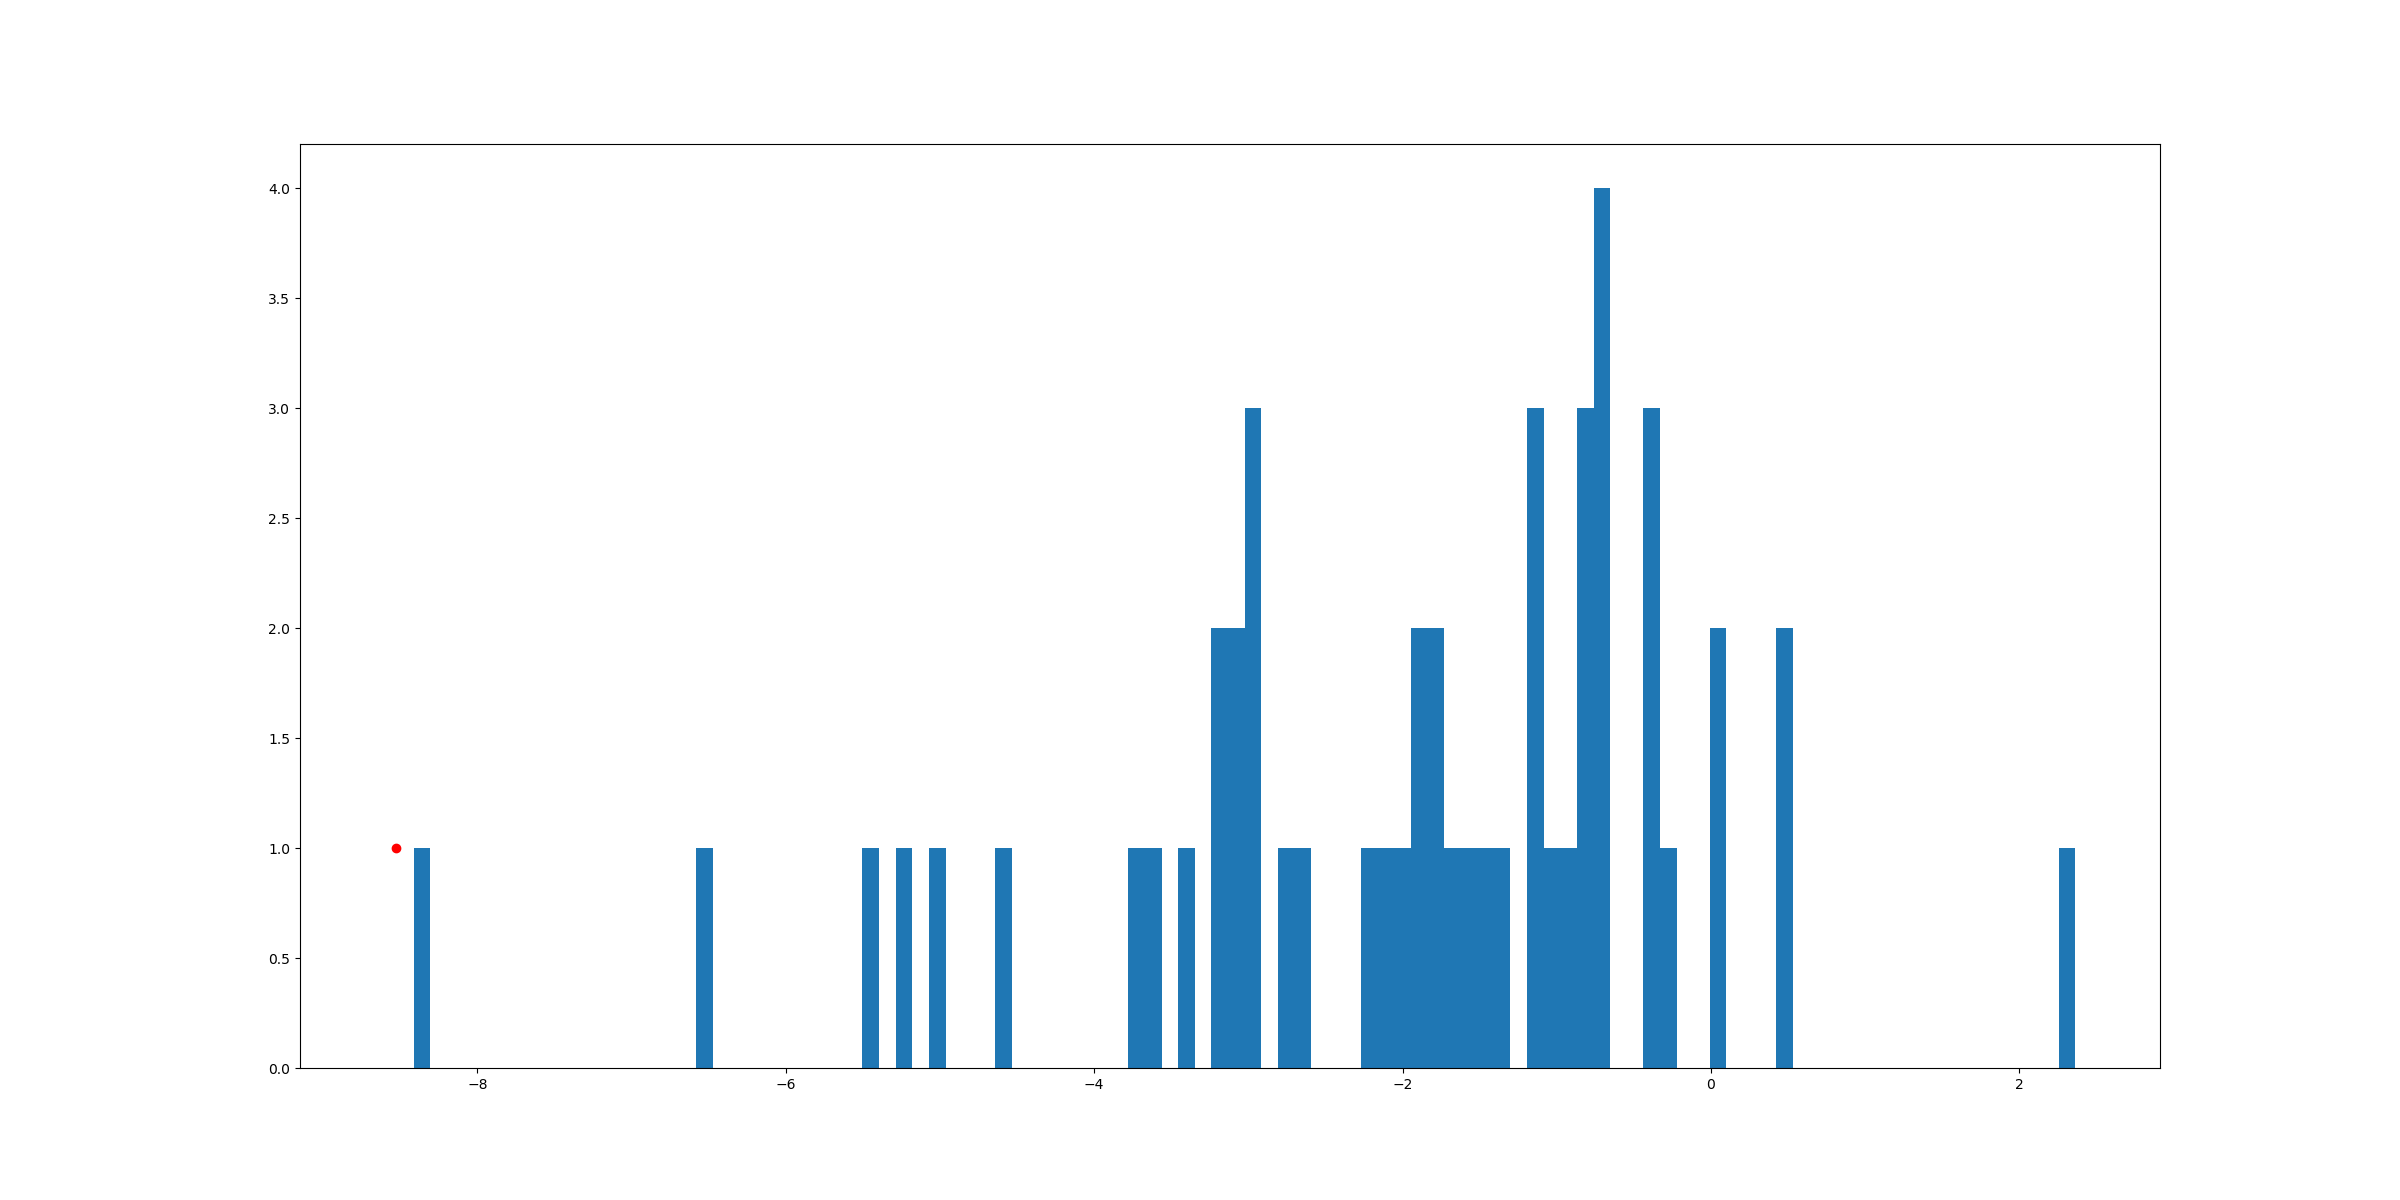
\includegraphics[trim=200 80 100 100, clip,width=12cm]{c2_figures/429-hist.png}
% \caption{Histogram of $0.7$-persistence of ImageNet examples with class "Baseball." ??DG?? Let's replace red dot with something more noticable like an x. Red dot on the left indicates the same $\sigma$ measurement for an adversarial perturbation of a "Rose-Hip" with new class "Baseball" \ref{fgsmhip}} 
% \label{imnetfgsmsamp}
% \end{figure}

% Much like the above case for MNIST, IGSM examples generated on ImageNet were much less $(\gamma,\sigma)$-stable than natural images. DG: Explain:?? 98\% of adversarial images could be distinguished by their $(\gamma,\sigma)$-stability. It should be noted that due to computational intensity of processing ImageNet samples, this dataset is significantly smaller than that used for the MNIST experiments. 

% \subsection{Effects of network complexity on persistence}
% %{Neighborhood sampling of L-BFGS adversarial examples for MNIST}

% As a further study into the relationship of network complexity with $(\gamma,\sigma)$-stability, we revisit the now classic work of \cite{Szegedy2013} on adversarial examples. In these experiments, we used L-BFGS technique from \cite{Szegedy2013} to prepare adversarial examples. The same networks and examples were be subjected to $0.7$-persistence analysis to determine any correspondence of stability with network accuracy and average distortion. 
% [??DG??: We need to define complexity and add it to the table]

% We also consider complexity of this type on convolutional DNNs, consisting of a composition of convolutional layers, followed by a truncation step that drops most of the results from the last convolutional layer, resulting in a low width layer, which is followed by some fully connected layers. 
%In our experiments, 
%a typical network is denoted ``C-Ch-$k$,'' where C reflects that this is a convolutional DNN, Ch denotes the number of channels and $k$ denotes the width of the smallest level, for instance, ``C-128-2''. 
%The ``C'' indicates my convolutional framework. The 128 indicates the number of channels per convolutional layer. The 4714 indicates the number of outputs which are \emph{discarded} from the final layer. In this case, 128 channels in my convolutional structure yields 4716 total output dimensions from the final convolutional layer. Dropping 4714 of these leaves $k = 2$ values which will be passed into the fully connected component of the network. In this way, we can look at more complicated DNNs in the following two dimensions ???
% The network has the form:

% %\vspace{.4cm}

% \begin{tabular}{|l|l|l|l|l|l|}
% \hline
%      Layer & Type & Channels & Kernel & Stride & Output Shape \\
% \hline
%      0 & Image & 1 & NA & NA & $(1, 28, 28)$ \\
%      1 & Conv & 128 & $(5,5)$& $(1,1)$& $(128, 24, 24)$\\
%      2 & Conv & 128 & $(5,5)$& $(1,1)$& $(128, 20, 20)$\\
%      3 & Conv & 128 & $(5,5)$& $(1,1)$& $(128, 16, 16)$\\
%      4 & Conv & 128 & $(5,5)$& $(1,1)$& $(128, 12, 12)$\\
%      5 & Max Pool & 128 & $(2, 2)$ & $(2, 2)$& $(128, 6, 6)$ \\
%      6 & Trunc & 1 & NA & NA & $(k)$ \\
%      7 & FC & $(k, 256)$ & NA & NA & 256 \\
%      8 & FC & $(256, 10)$ & NA & NA & 10 \\
%      \hline
% \end{tabular}

% \noindent Where $k$ is a number of desired output parameters from the convolutional component. 
% [DG: What changes if the number of channels changes? Can we give a general form.]
% We denote such a network as ``C-Ch-$k$,'' where C reflects that this is a convolutional DNN, Ch denotes the number of channels and $k$ denotes the width of the smallest level, for instance, ``C-128-2''.

% %\subsubsection{Re-examining Szegedy Results with sampling}

% Table \ref{table1} is a recreation of \cite[Table 1]{Szegedy2013} in which networks of differing complexity are trained and attacked using L-BFGS. In addition to recreating the results from \cite{Szegedy2013}, the table contains columns for the average $0.7$-persistence natural and adversarial examples for each network. The networks listed are FC10-4, a fully connected network with no hidden layers that that takes the input vector $x \in \RR^{784}$ to an output vector of $y \in \RR^{10}$ with the $\lambda*\Norm{w}_2/N$ where $\lambda = 10^{-4}$ and $N$ is the number of parameters in $w$) added as regularization to the objective function during training. FC10-2 is the same except with $\lambda = 10^{-2}$ and FC10-0 has $\lambda=1$ (a very large coefficient for regularization). FC100-100-10 and FC200-200-10 are networks with 2 hidden layers with regularization added for each layer of perceptrons with the $\lambda$ for each layer equal to $10^{-5}, 10^{-5}$, and  $10^{-6}$. Training for these networks is conducted with a fixed number of epochs. 

% \begin{table}[pt]
% \centering
% \caption{Recreation of ~\cite[Table 1]{Szegedy2013} using pytorch. New columns show average $0.7$-persistence values for adversarial and natural examples. DG: Needs more description??}
% \label{table1}
% \begin{tabular}{llllll}
% \toprule
% Network & Test Acc & Avg Dist & Success Pct & Persist (Nat) & Persist (Adv) \\
% \midrule
% FC10-4 & 92.09 & 0.123 & ?? & 0.93 & 1.68\\
% FC10-2 & 90.77 & 0.178 & ?? & 1.37 & 4.25\\
% FC10-0 & 86.89 & 0.278 & ?? & 1.92 & 12.22\\
% FC100-100-10 & 97.31 & 0.086 & ?? & 0.65 & 0.56 \\
% FC200-200-10 & 97.61 & 0.087 & ?? & 0.73 & 0.56 \\
% \midrule
% C-2-0 & 95.94 & 0.09 & 61.64 & 3.33 & 0.027 \\
% C-4-0 & 97.36 & 0.12 & 81.81 & 0.35 & 0.027 \\
% C-8-0 & 98.50 & 0.11 & 85.47 & NA & 0.0517 \\
% C-16-0 & 98.90 & 0.11 & 88.03 & 0.53 & 0.0994 \\
% C-32-0 & 98.96 & 0.11 & 86.23 & 0.78 & 0.0836 \\
% C-64-0 & 99.00 & 0.10 & 89.74 & 0.81 & 0.0865 \\
% C-128-0 & 99.17 & 0.11 & 87.87 & 0.77 & 0.0883 \\
% C-256-0 & 99.09 & 0.11 & 83.04 & 0.83 & 0.0900 \\
% C-512-0 & 99.22 & 0.10 & 88.88 & 0.793 & 0.0929 \\
% %C-128-2000 & 99.07 & 0.11 & 89.27 & 0.731 & 0.136 \\
% %C-128-4000 & 99.13 & 0.098 & 89.71 & 1.024 & 0.424 \\
% %C-128-4500 & 99.32 & 0.096 & 90.59 & NA & 0.103 \\
% %C-128-4700 & 97.48 & 0.079 & 87.16 & NA & NA \\
% %C-128-4708 & 95.69 & 0.077 & 80.90 & 0.15 & 0.0307 \\
% %C-128-4712 & 93.04 & 0.135 & 57.11 & 0.14 & 0.0296 \\
% %C-128-4714 & 78.87 & 0.211 & 41.61 & 0.059 & 0.012 \\
% %C-128-4715 & 65.99 & 0.831 & 23.61 & NA & 0.0092 \\ \hline
% \bottomrule
% \end{tabular}
% \end{table}
% DG: Why do we need distortion diagram???
% \begin{figure}[p]
% 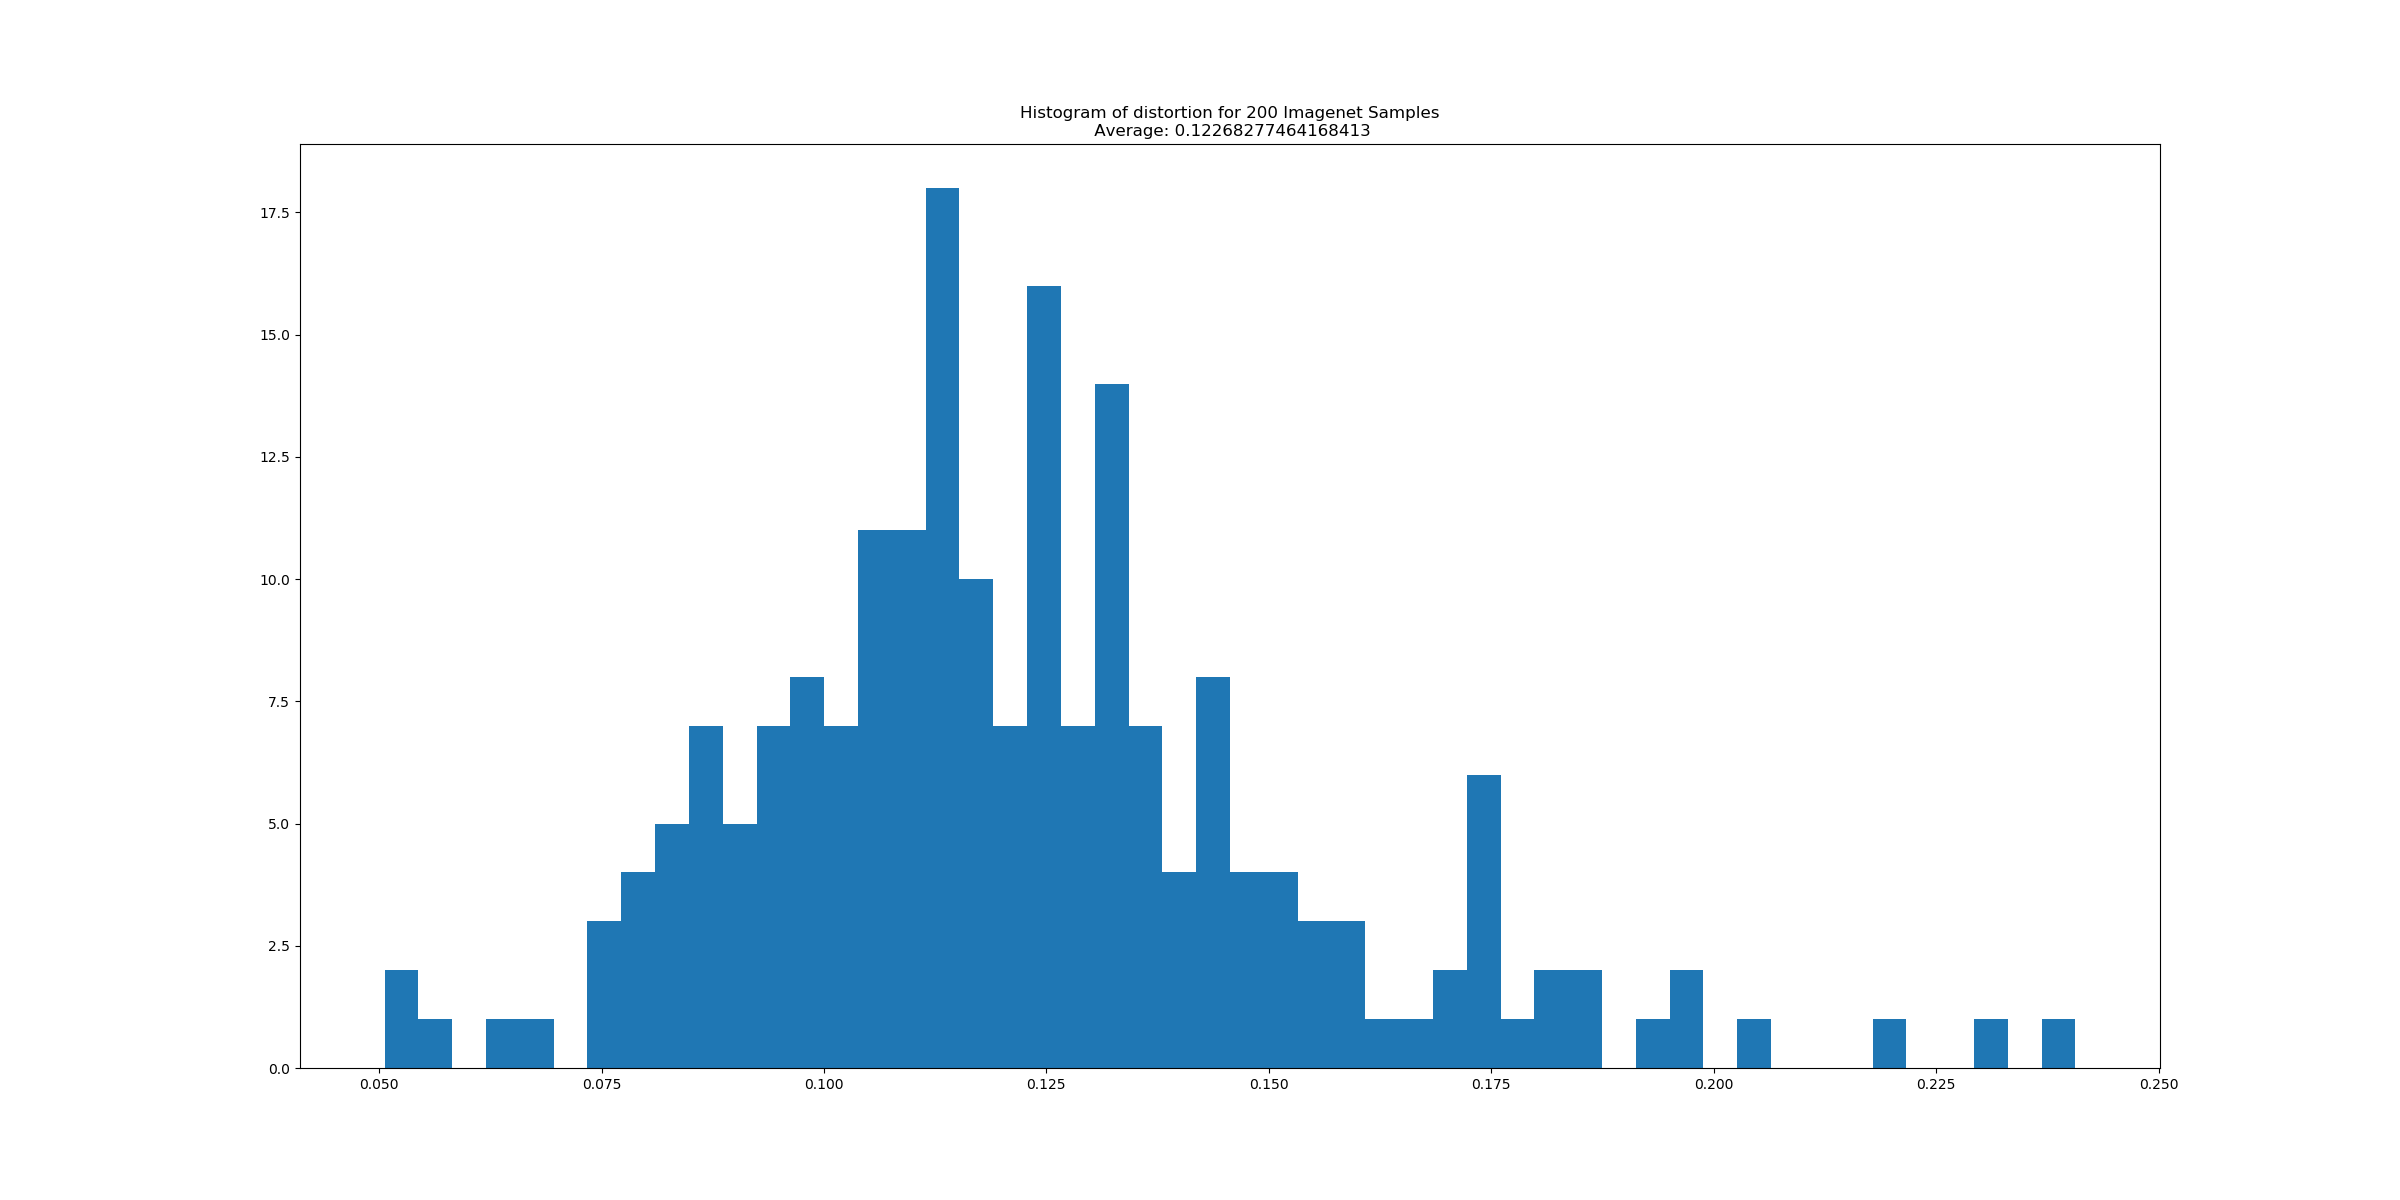
\includegraphics[trim=200 80 100 100, clip,width=7cm]{c2_figures/FC10-4-distortion_hist.png}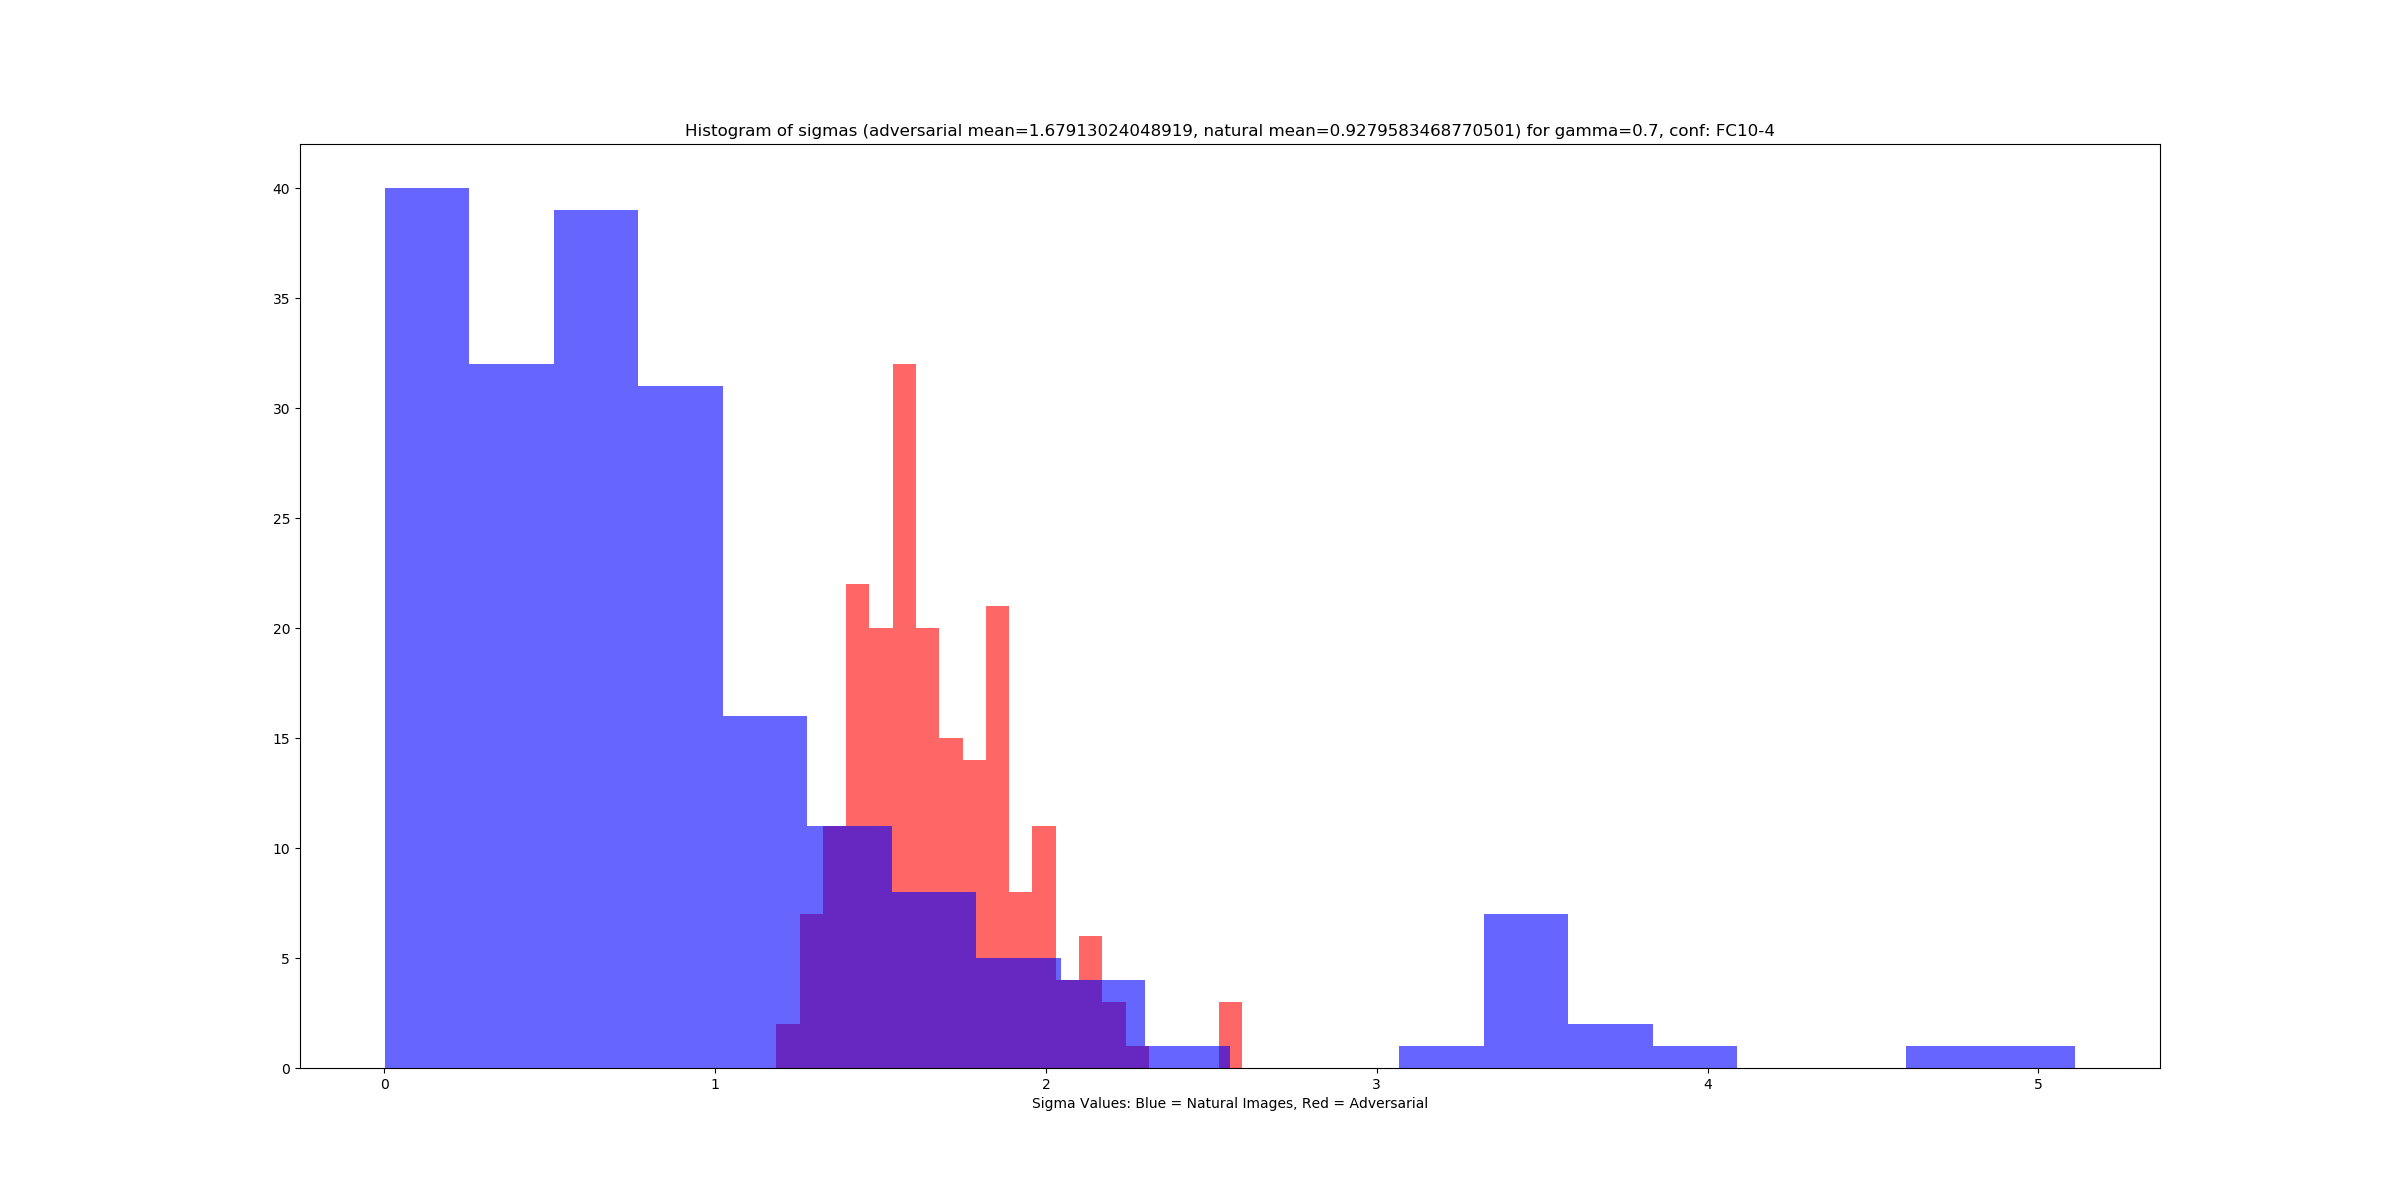
\includegraphics[trim=200 80 100 100, clip,width=7cm]{c2_figures/FC10-4-gamma1_hist.png}
% \caption{Distortion (left) and $0.7$-persistence (right) for FC-10-4 in Table \ref{table1}}
% \label{table1hist1}
% \end{figure}
% \begin{figure}[pt]
% 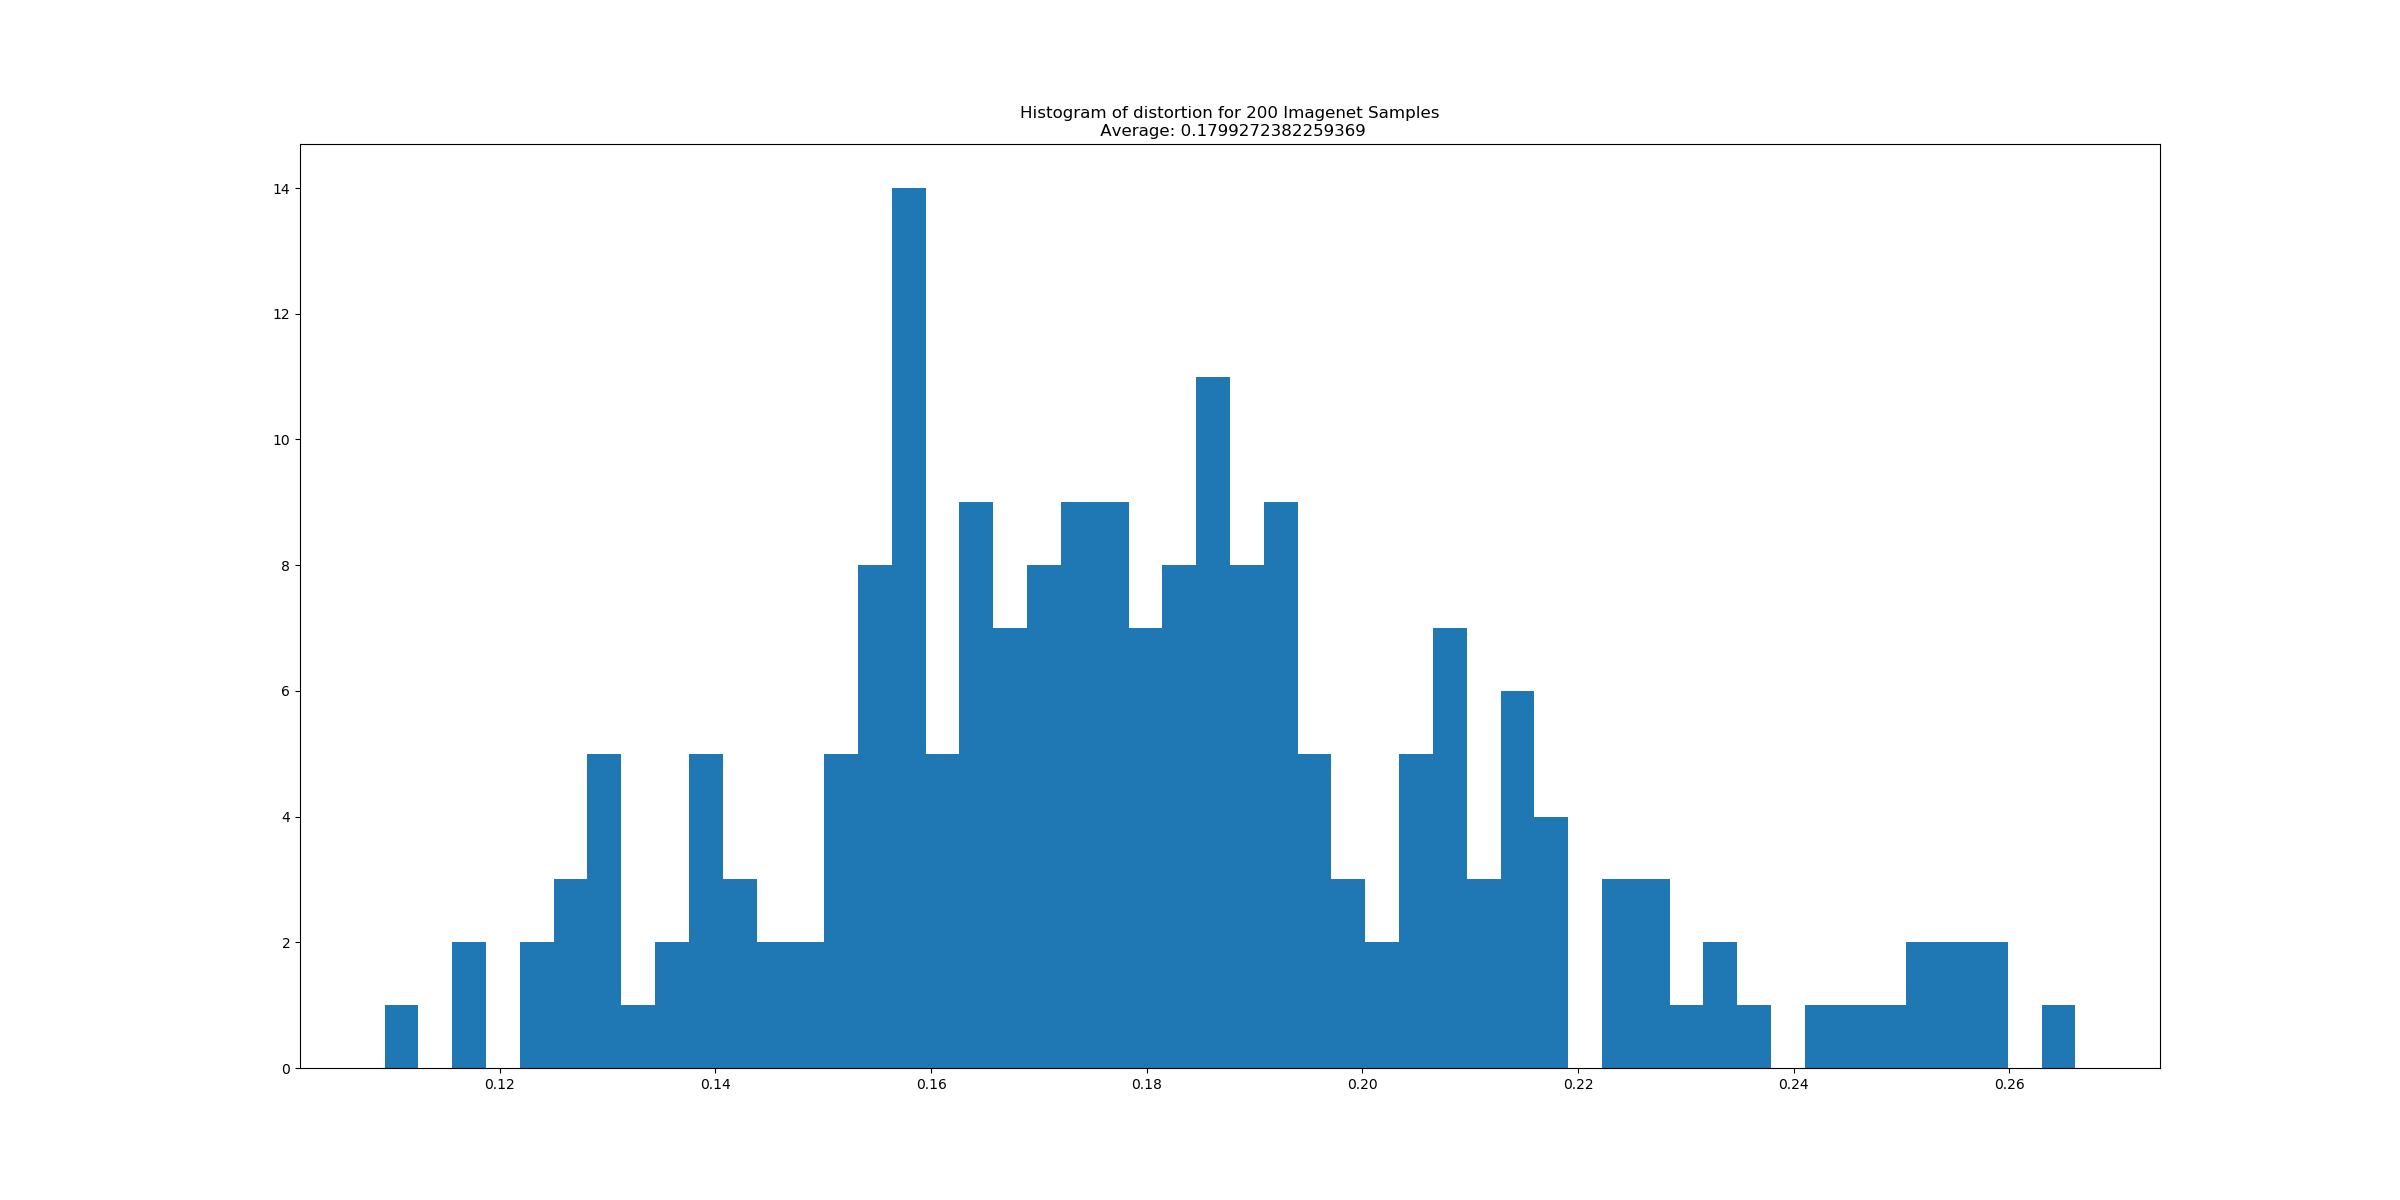
\includegraphics[trim=200 80 100 100, clip,width=7cm]{c2_figures/FC10-2-distortion_hist.png}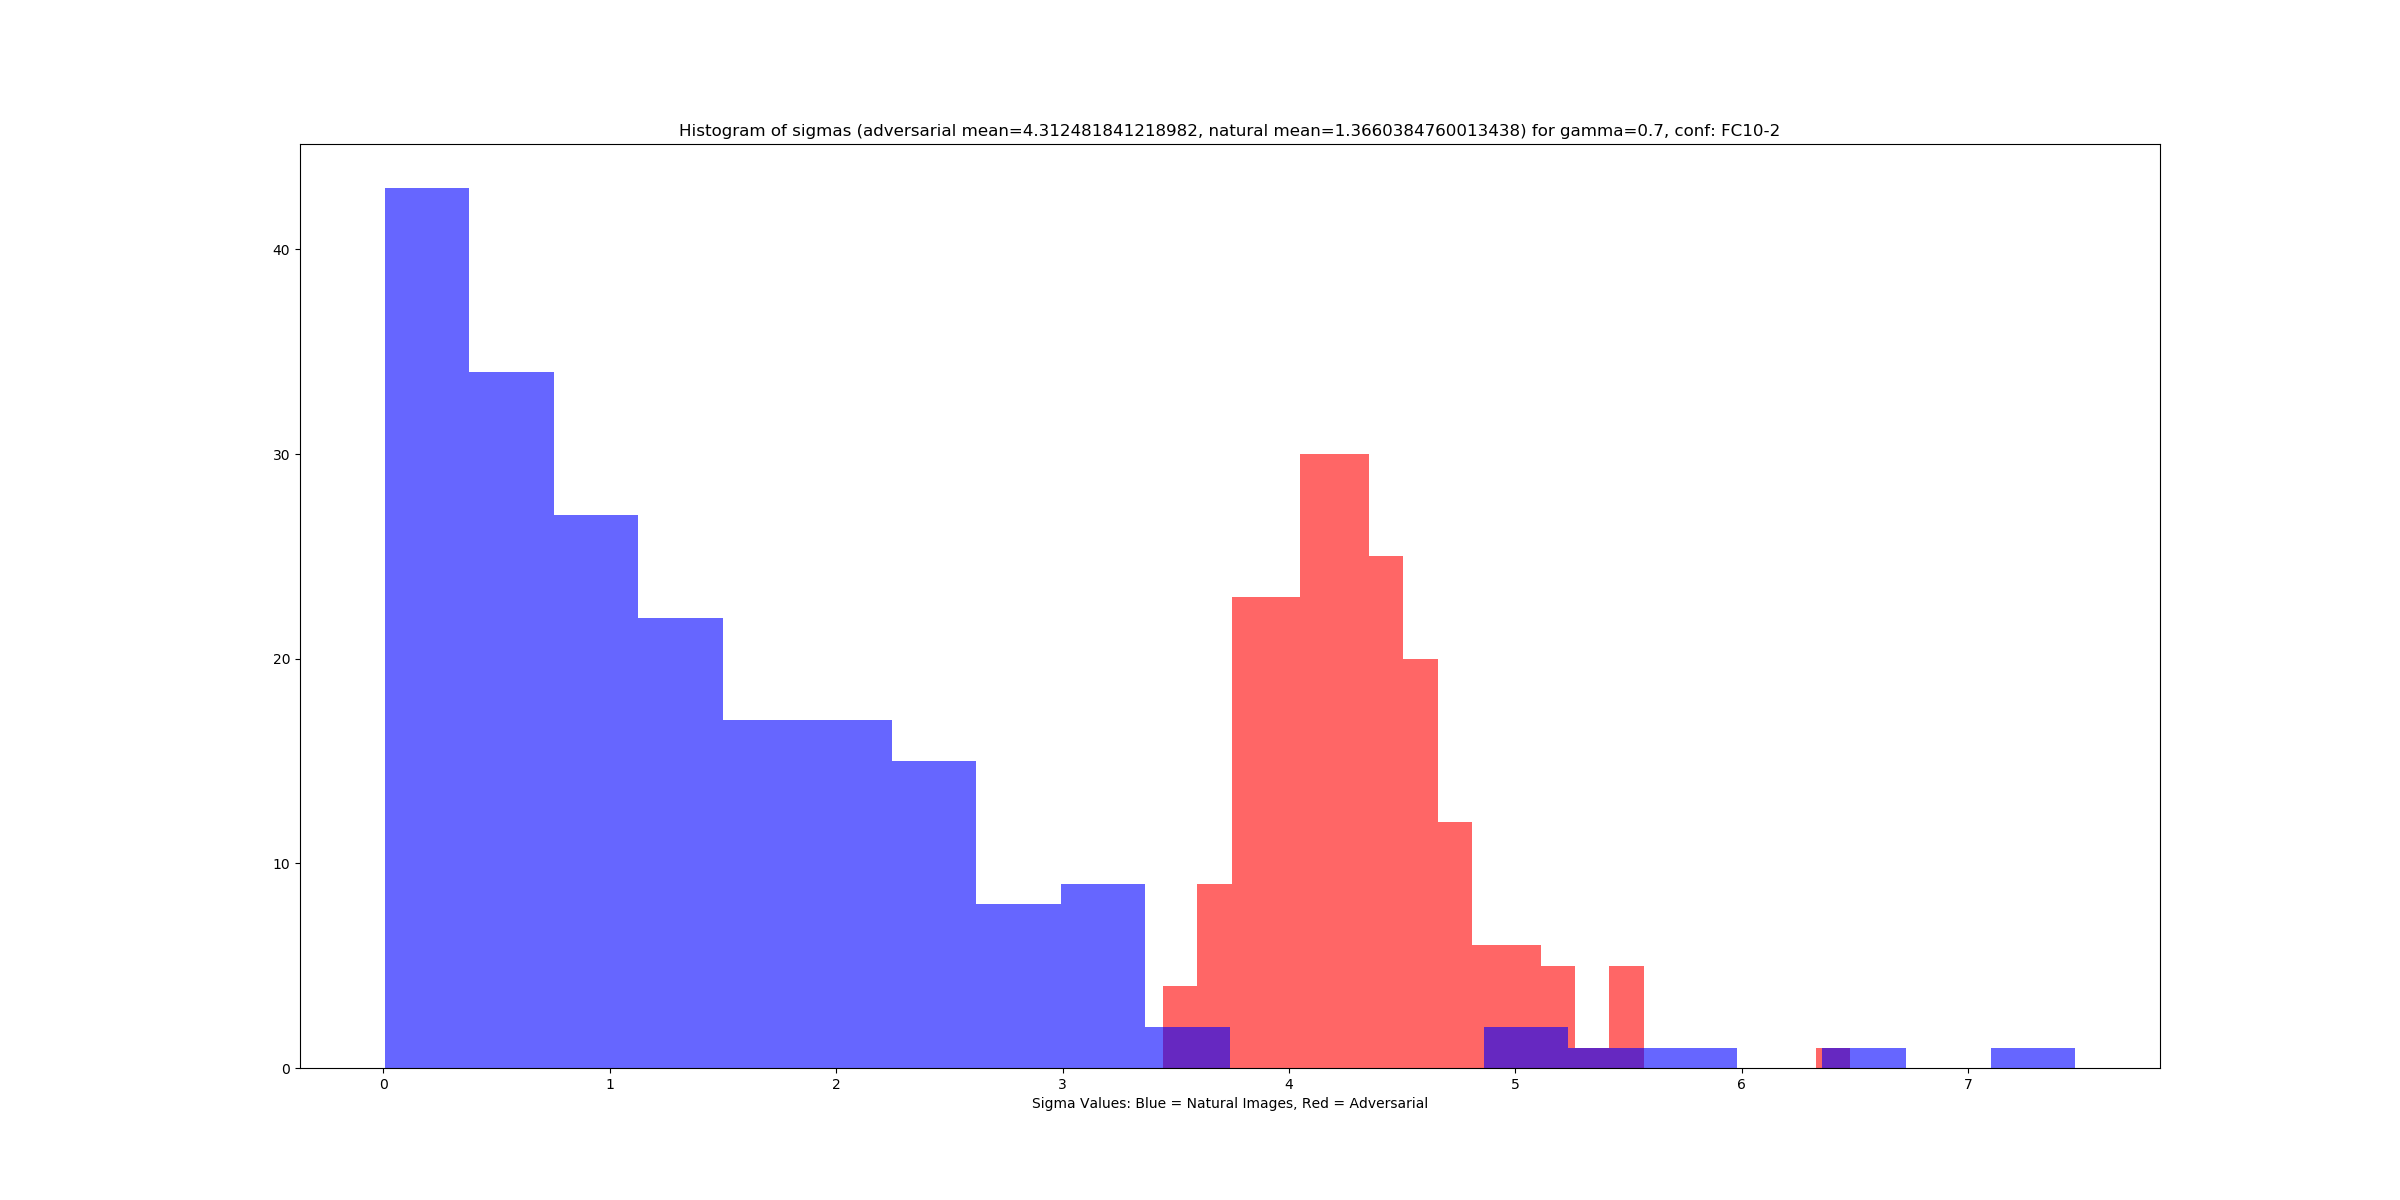
\includegraphics[trim=200 80 100 100, clip,width=7cm]{c2_figures/FC10-2-gamma1_hist.png}
% \caption{Distortion (left) and $0.7$-persistence (right) for FC10-2 in Table \ref{table1}}
% \label{table1hist2}
% \end{figure}
% \begin{figure}[p]
% 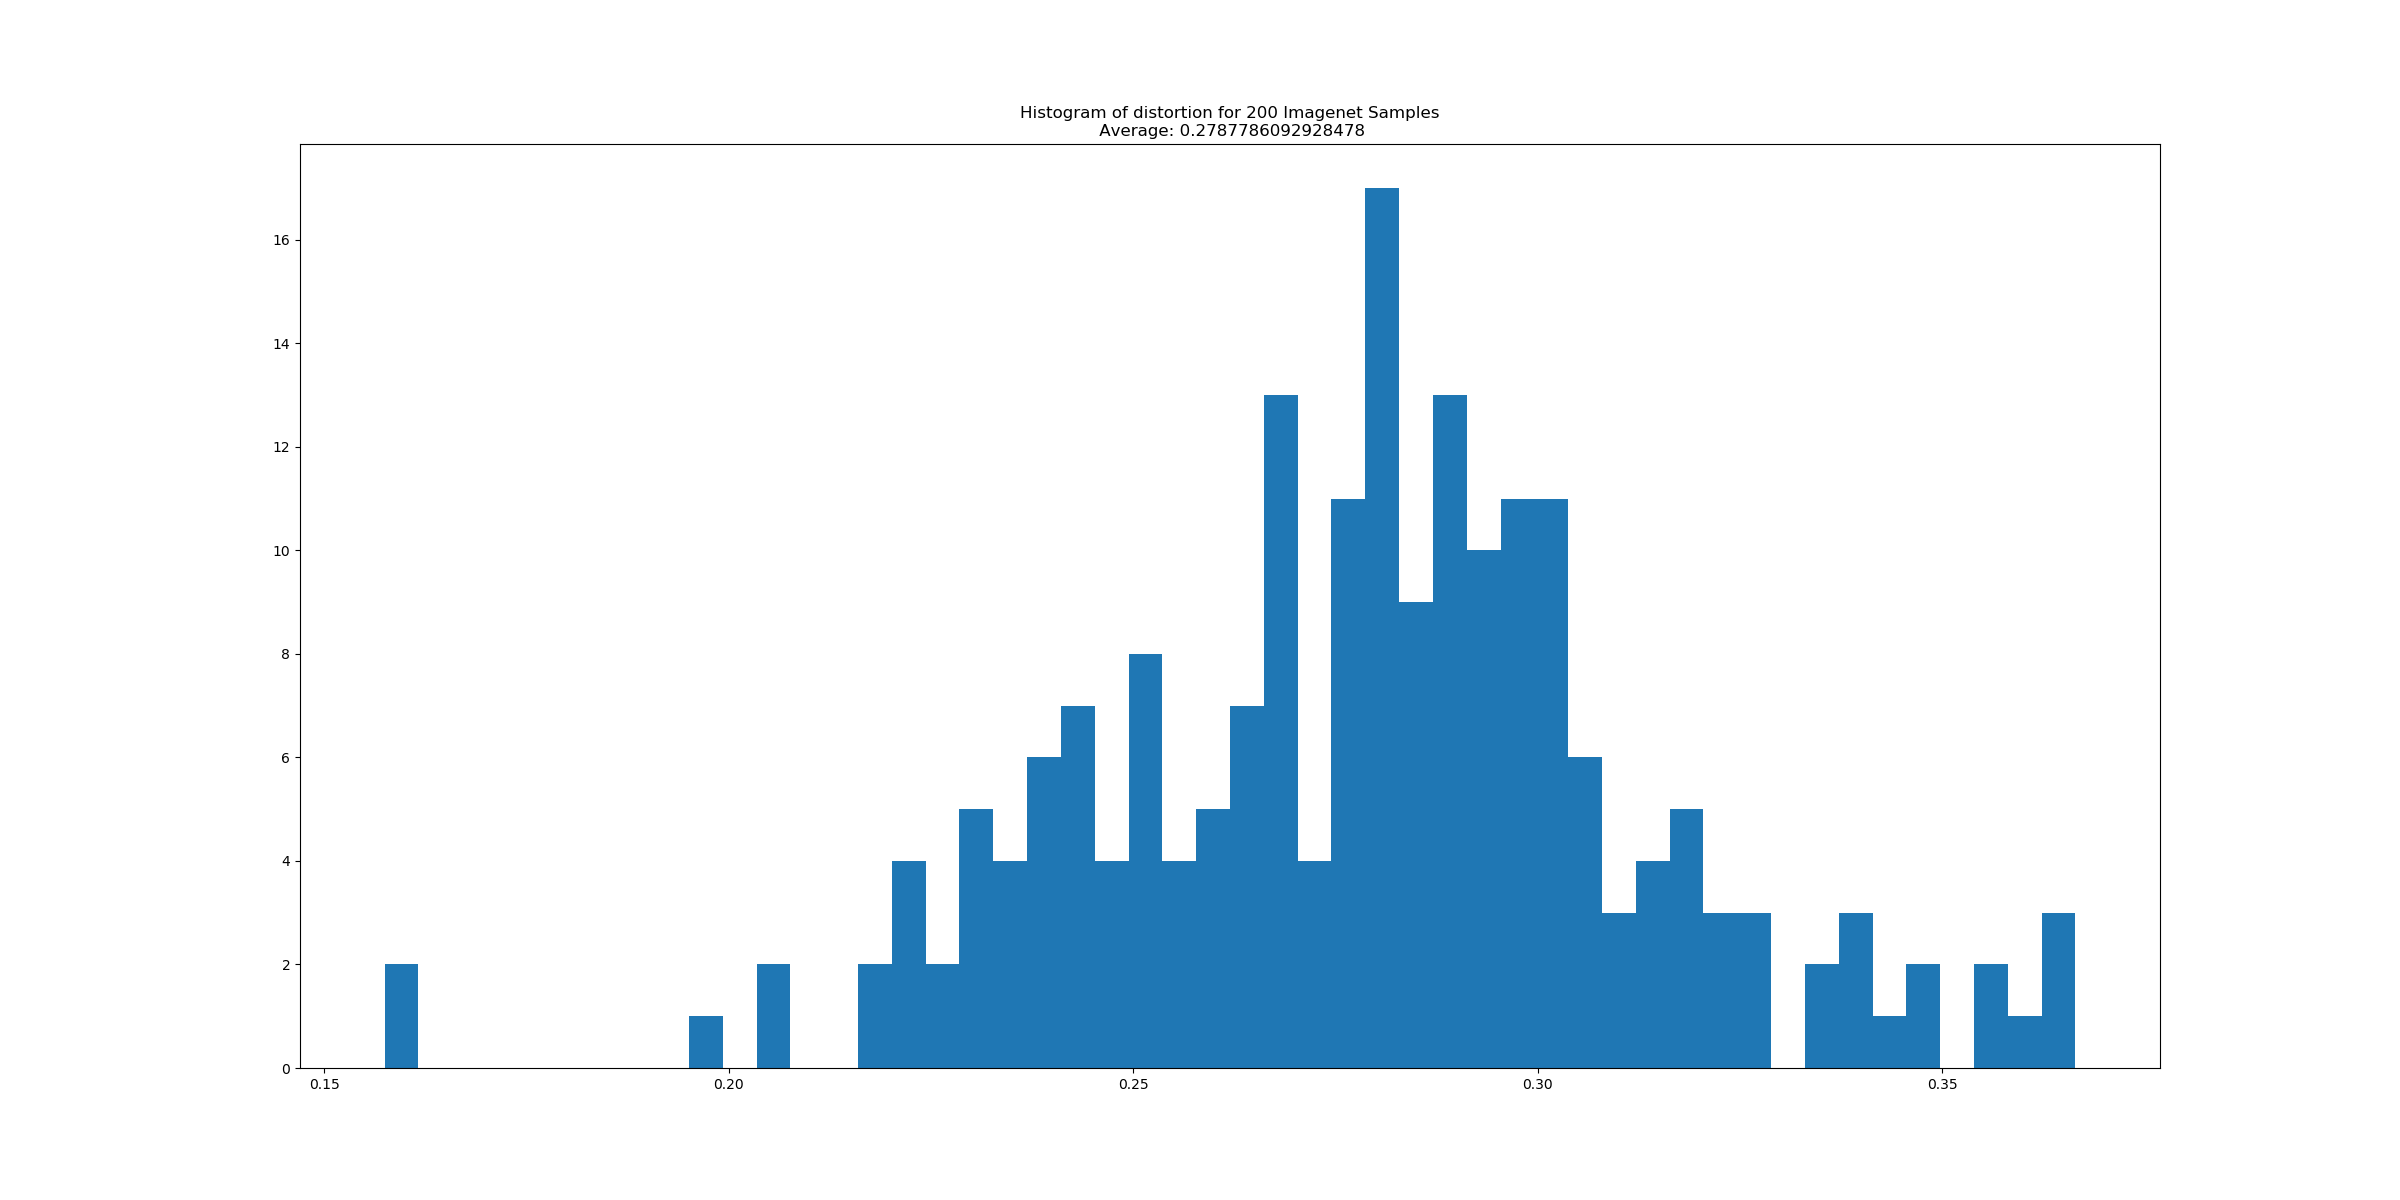
\includegraphics[trim=200 80 100 100, clip,width=7cm]{c2_figures/FC10-0-distortion_hist.png}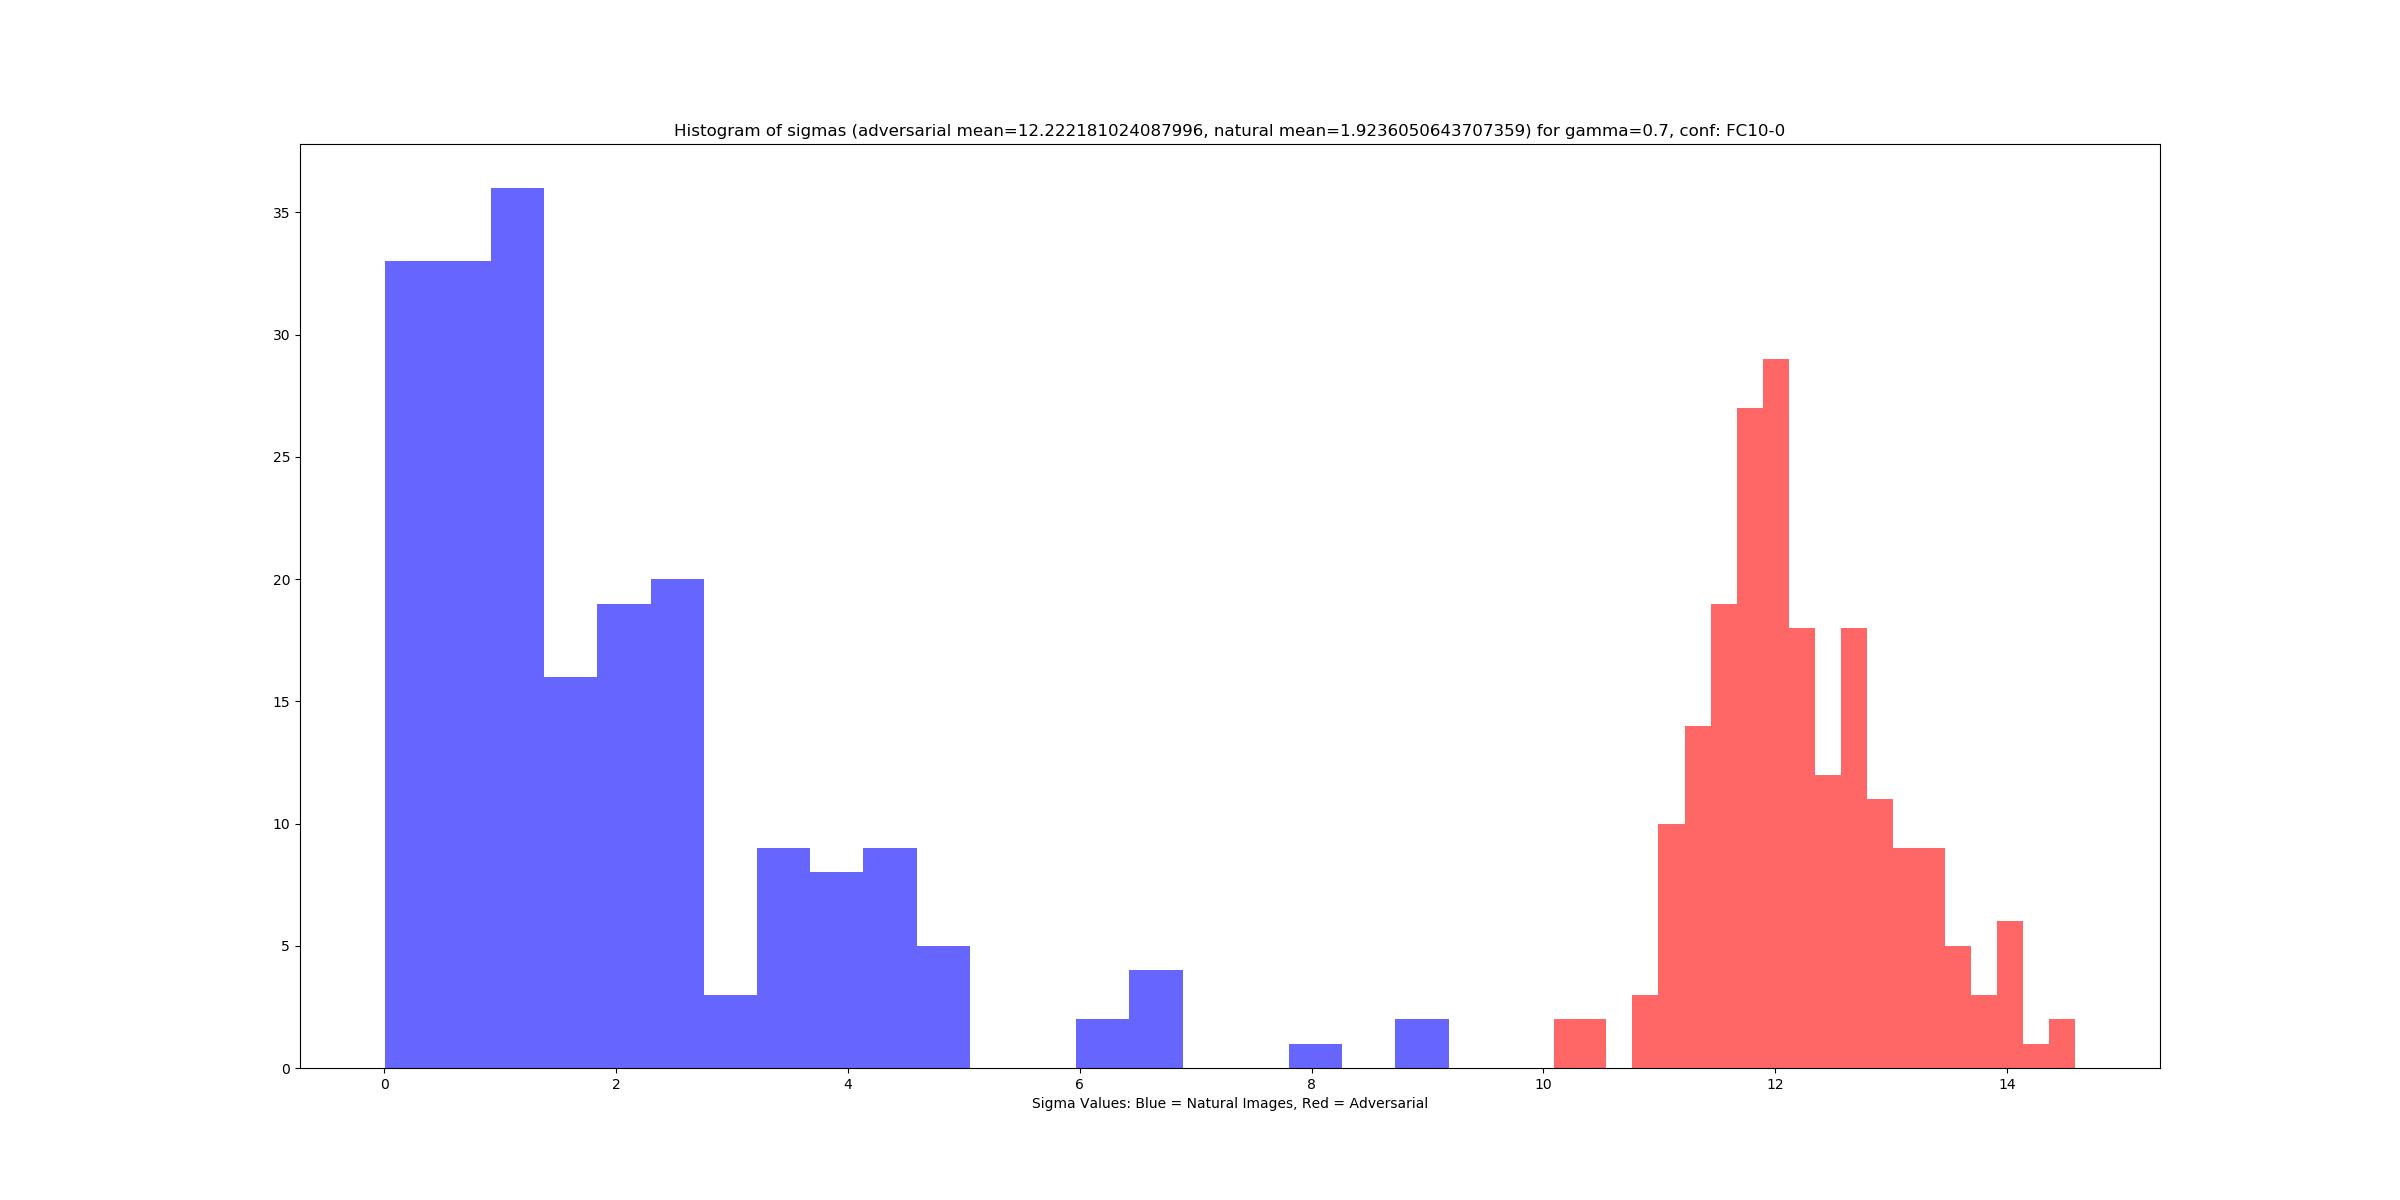
\includegraphics[trim=200 80 100 100, clip,width=7cm]{c2_figures/FC10-0-gamma1_hist.png}
% \caption{Distortion (left) and $0.7$-persistence (right) for FC10-0 in Table \ref{table1}}
% \label{table1hist3}
% \end{figure}
% \begin{figure}[p]
% 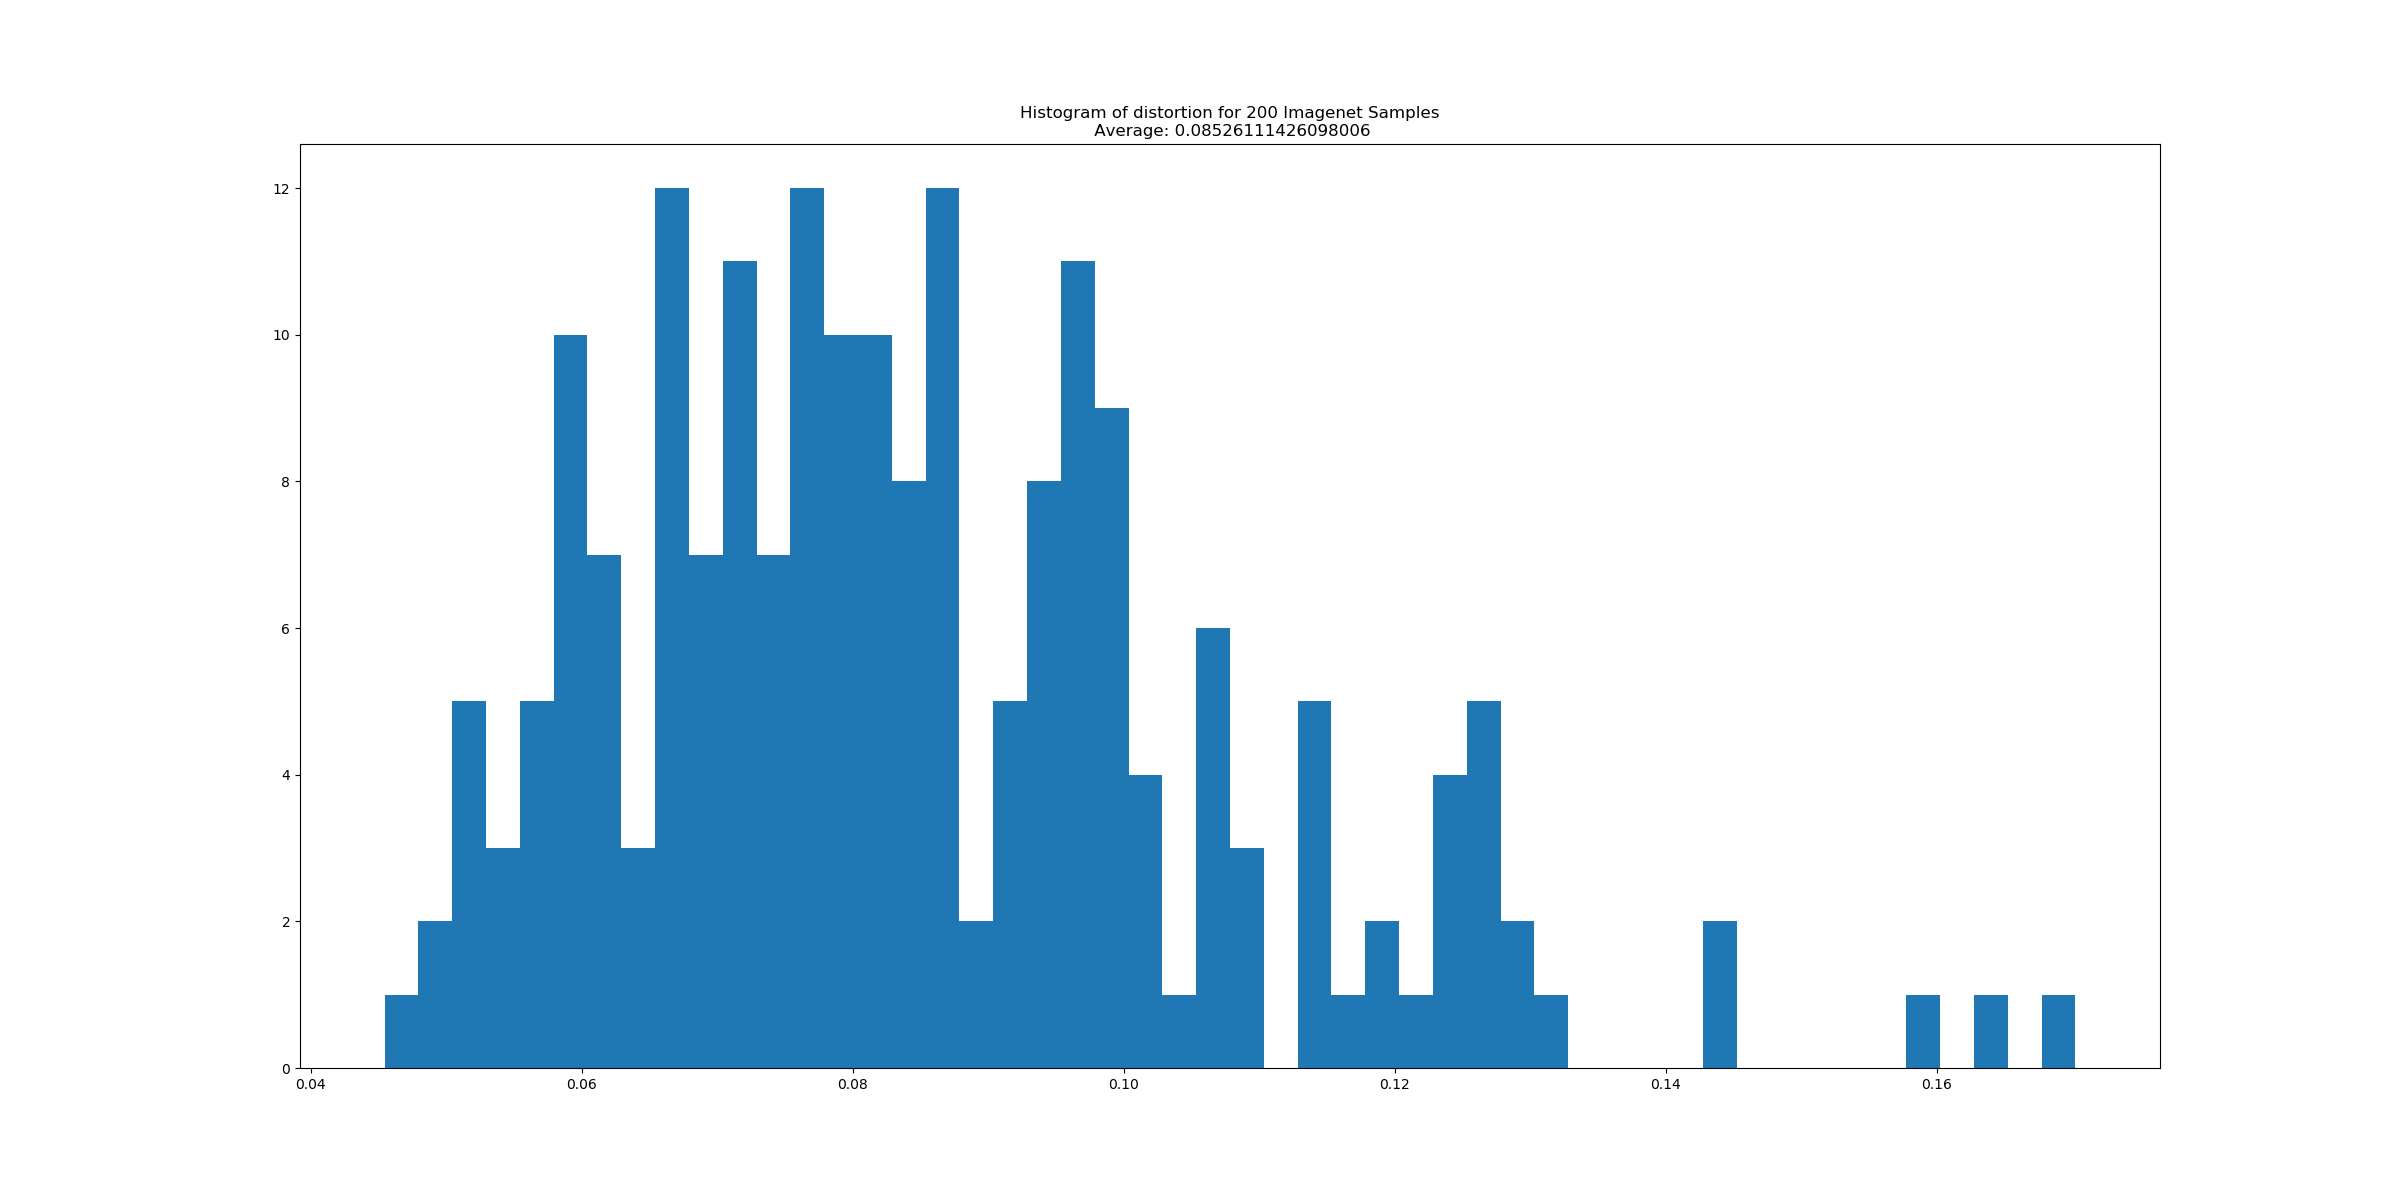
\includegraphics[trim=200 80 100 100, clip,width=7cm]{c2_figures/FC100-100-10-distortion_hist.png}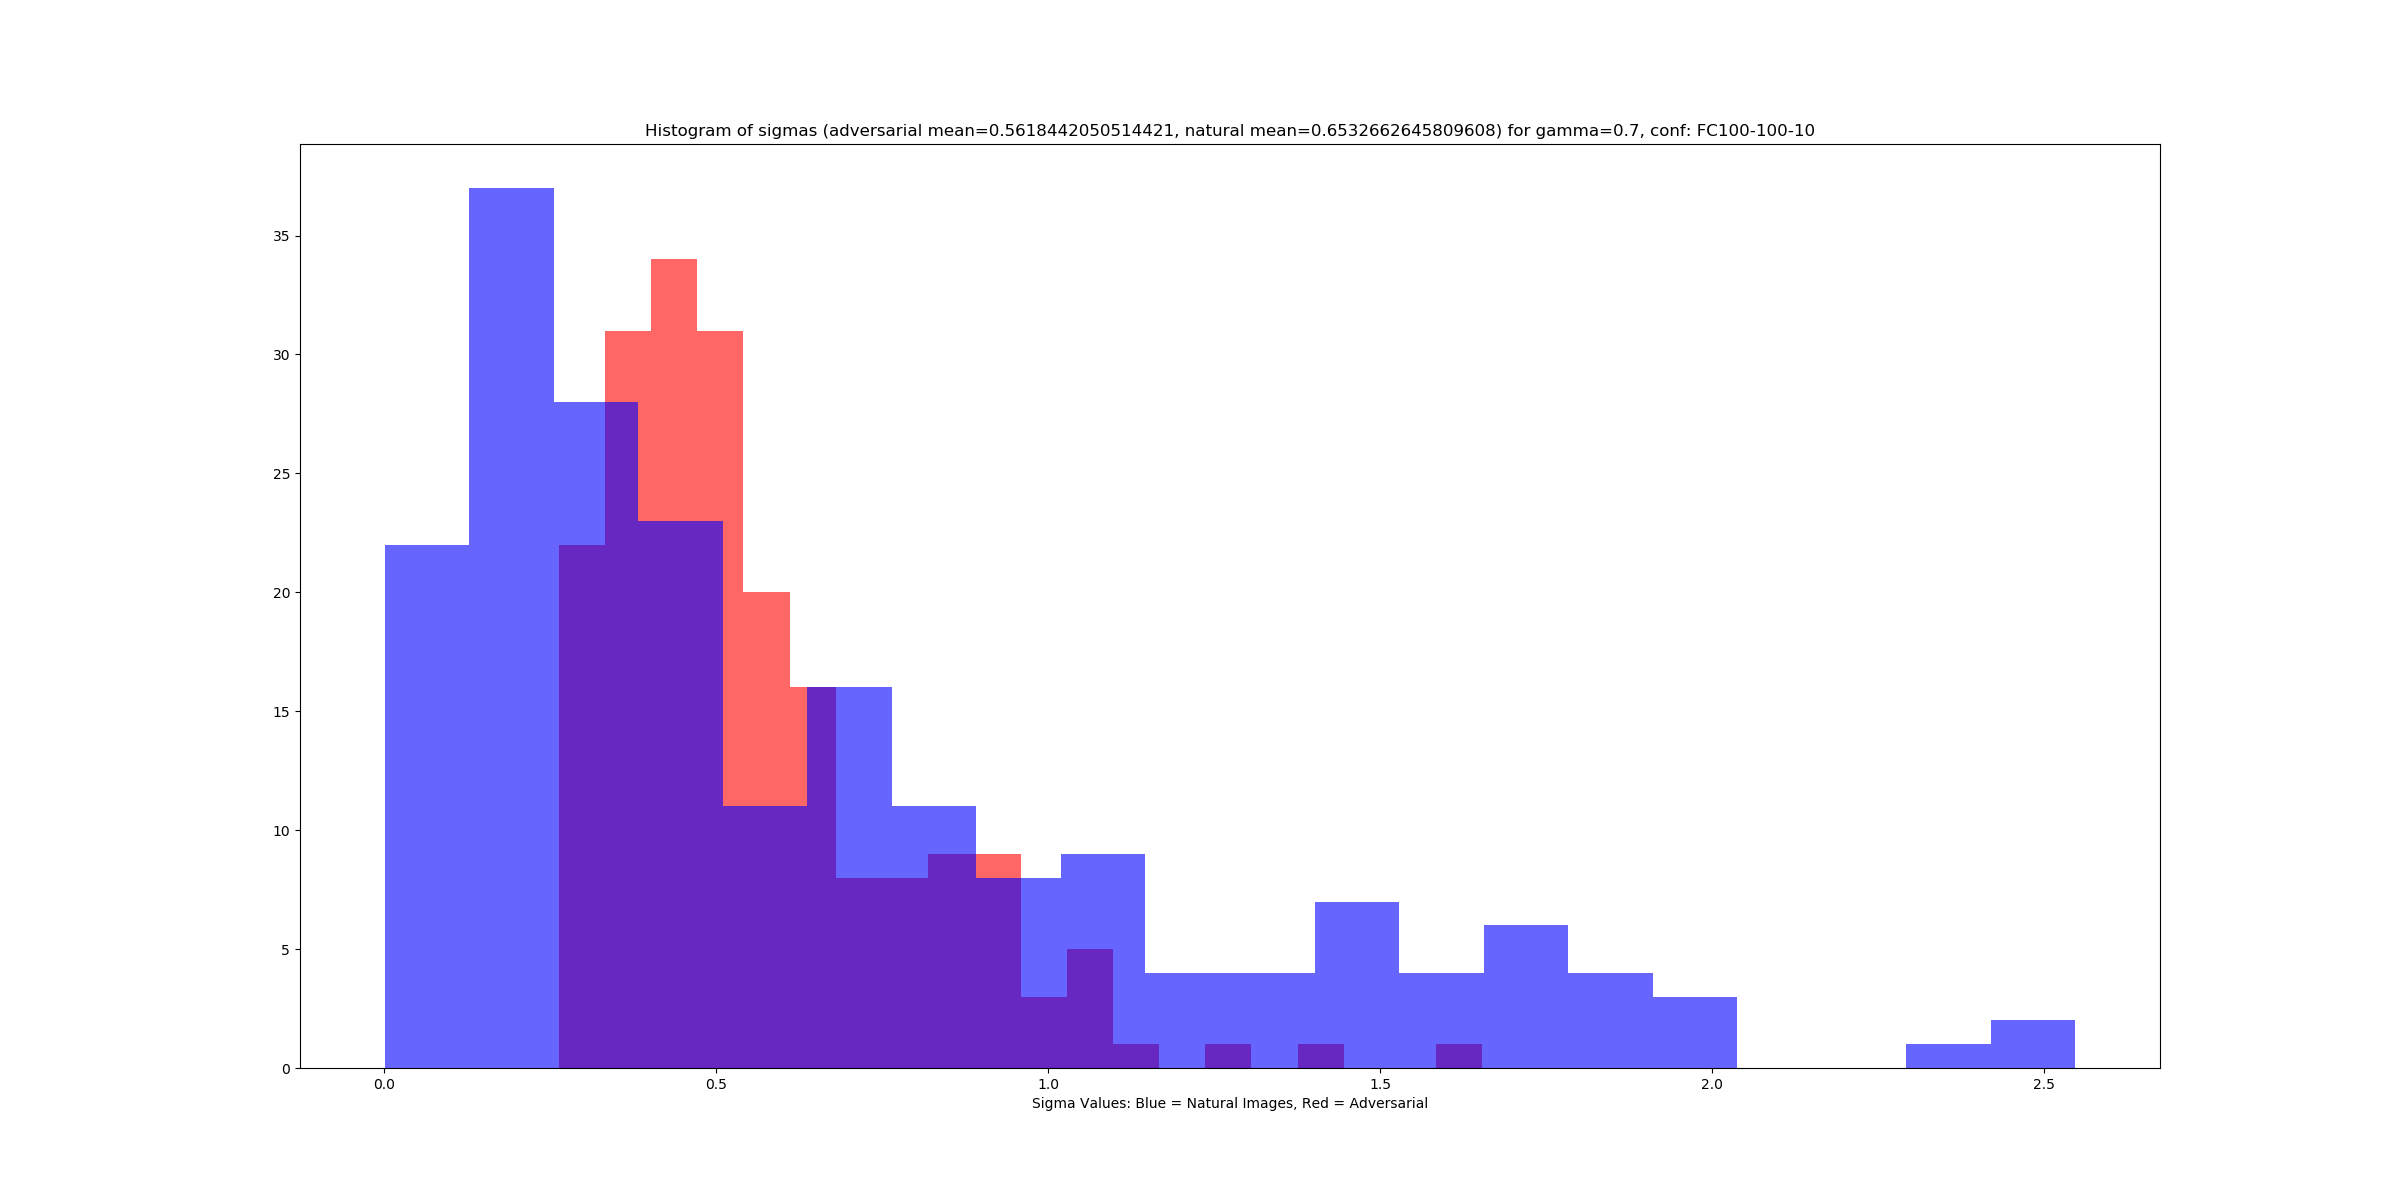
\includegraphics[trim=200 80 100 100, clip,width=7cm]{c2_figures/FC100-100-10-gamma1_hist.png}
% \caption{Distortion (left) and $0.7$-persistence (right) for FC100-100-10 in Table \ref{table1}}
% \label{table1hist4}
% \end{figure}
% \begin{figure}[p]
% 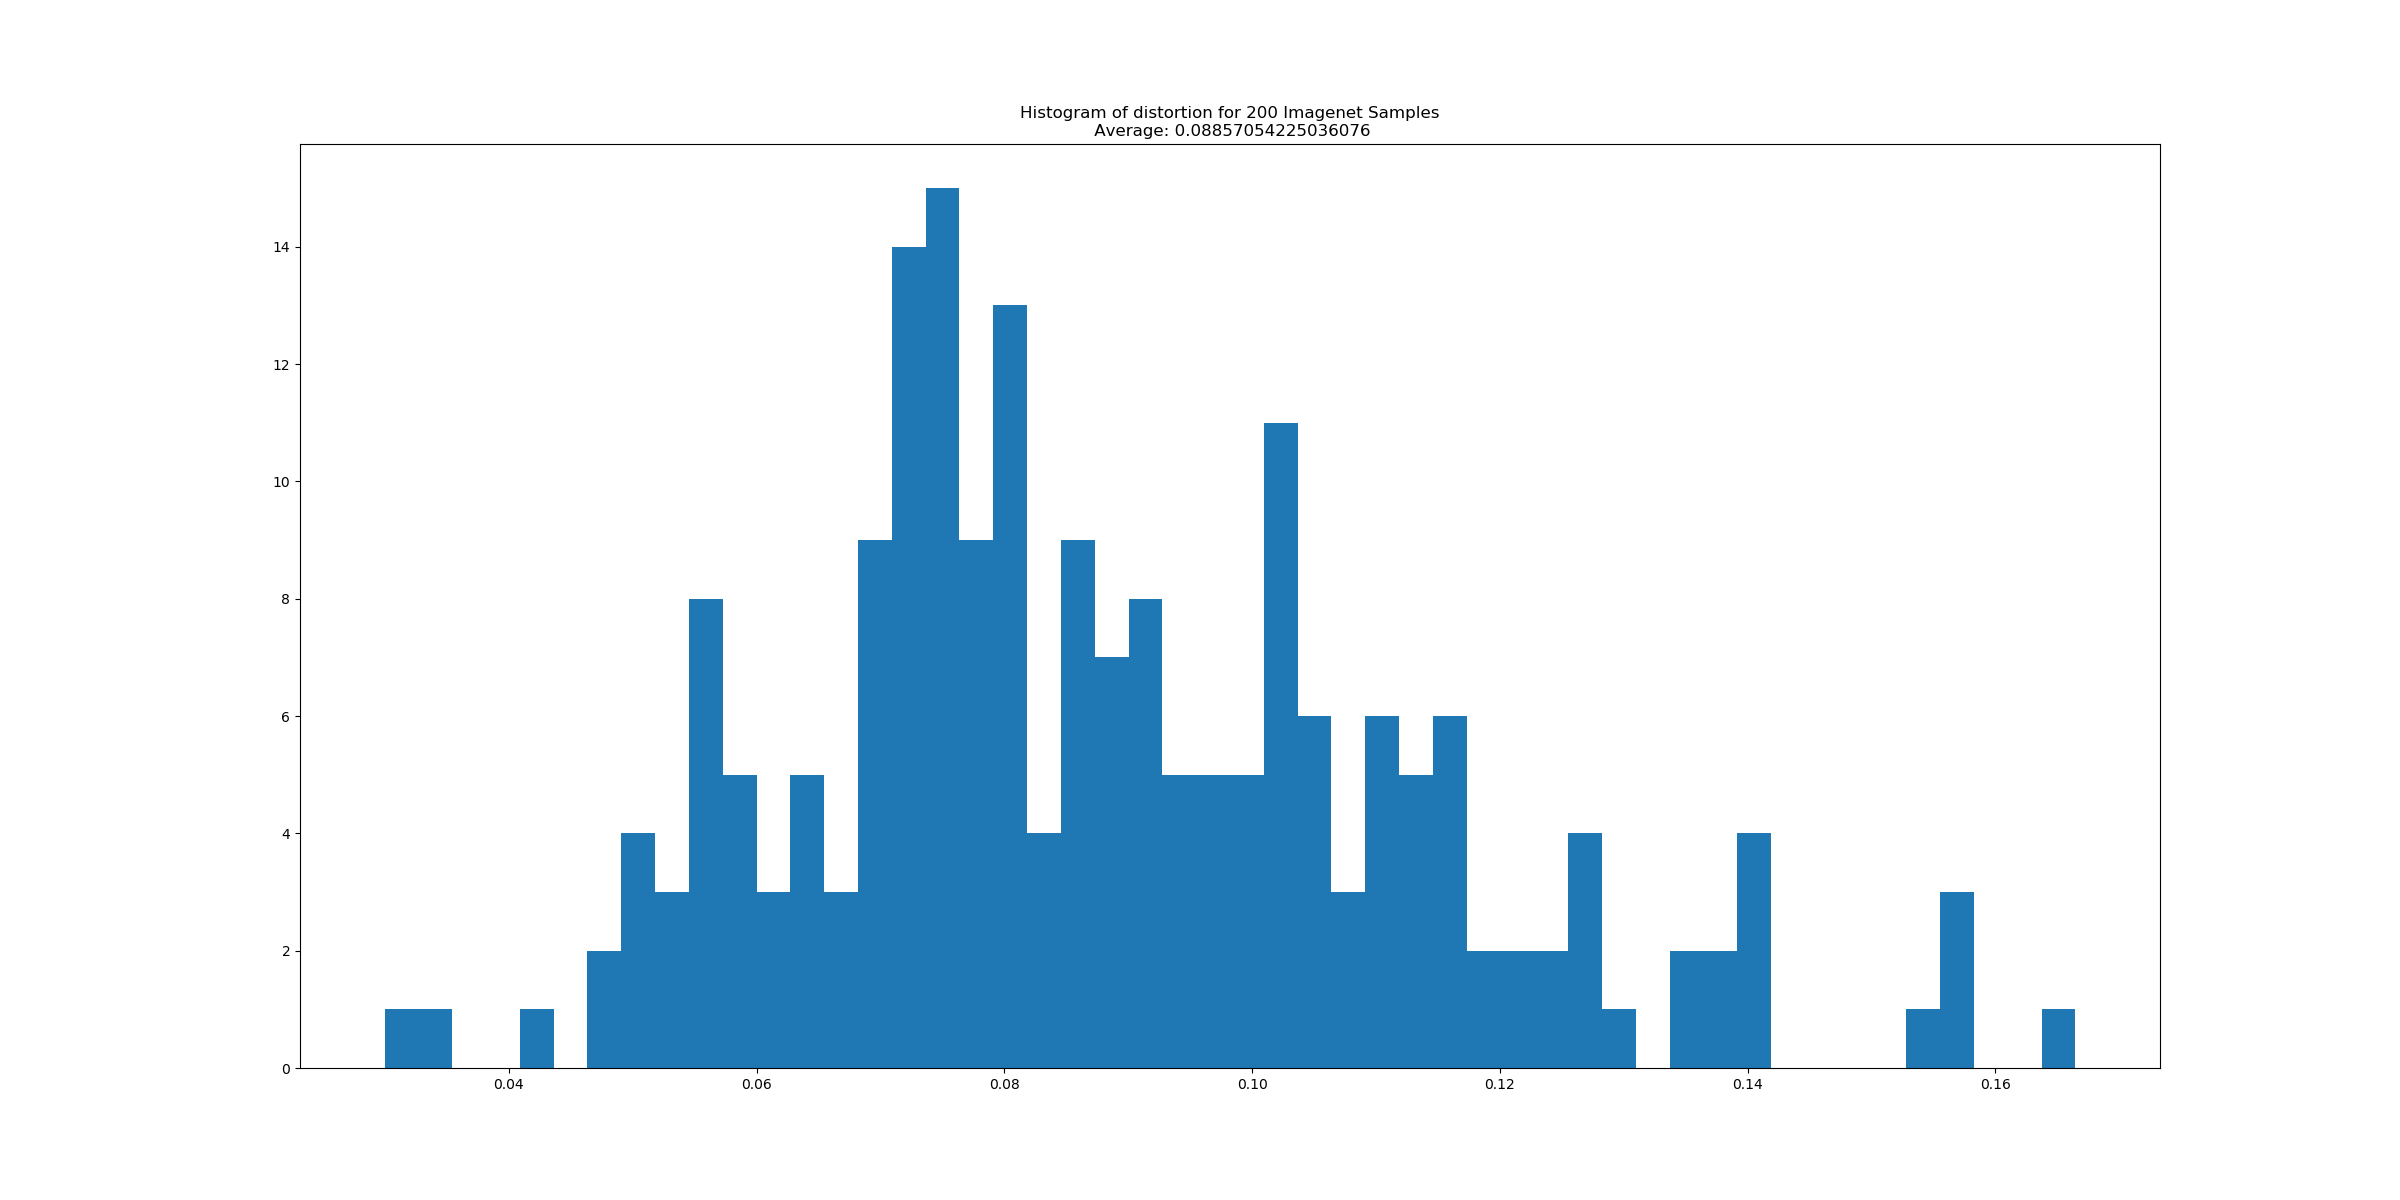
\includegraphics[trim=200 80 100 100, clip,width=7cm]{c2_figures/FC200-200-10-distortion_hist.png}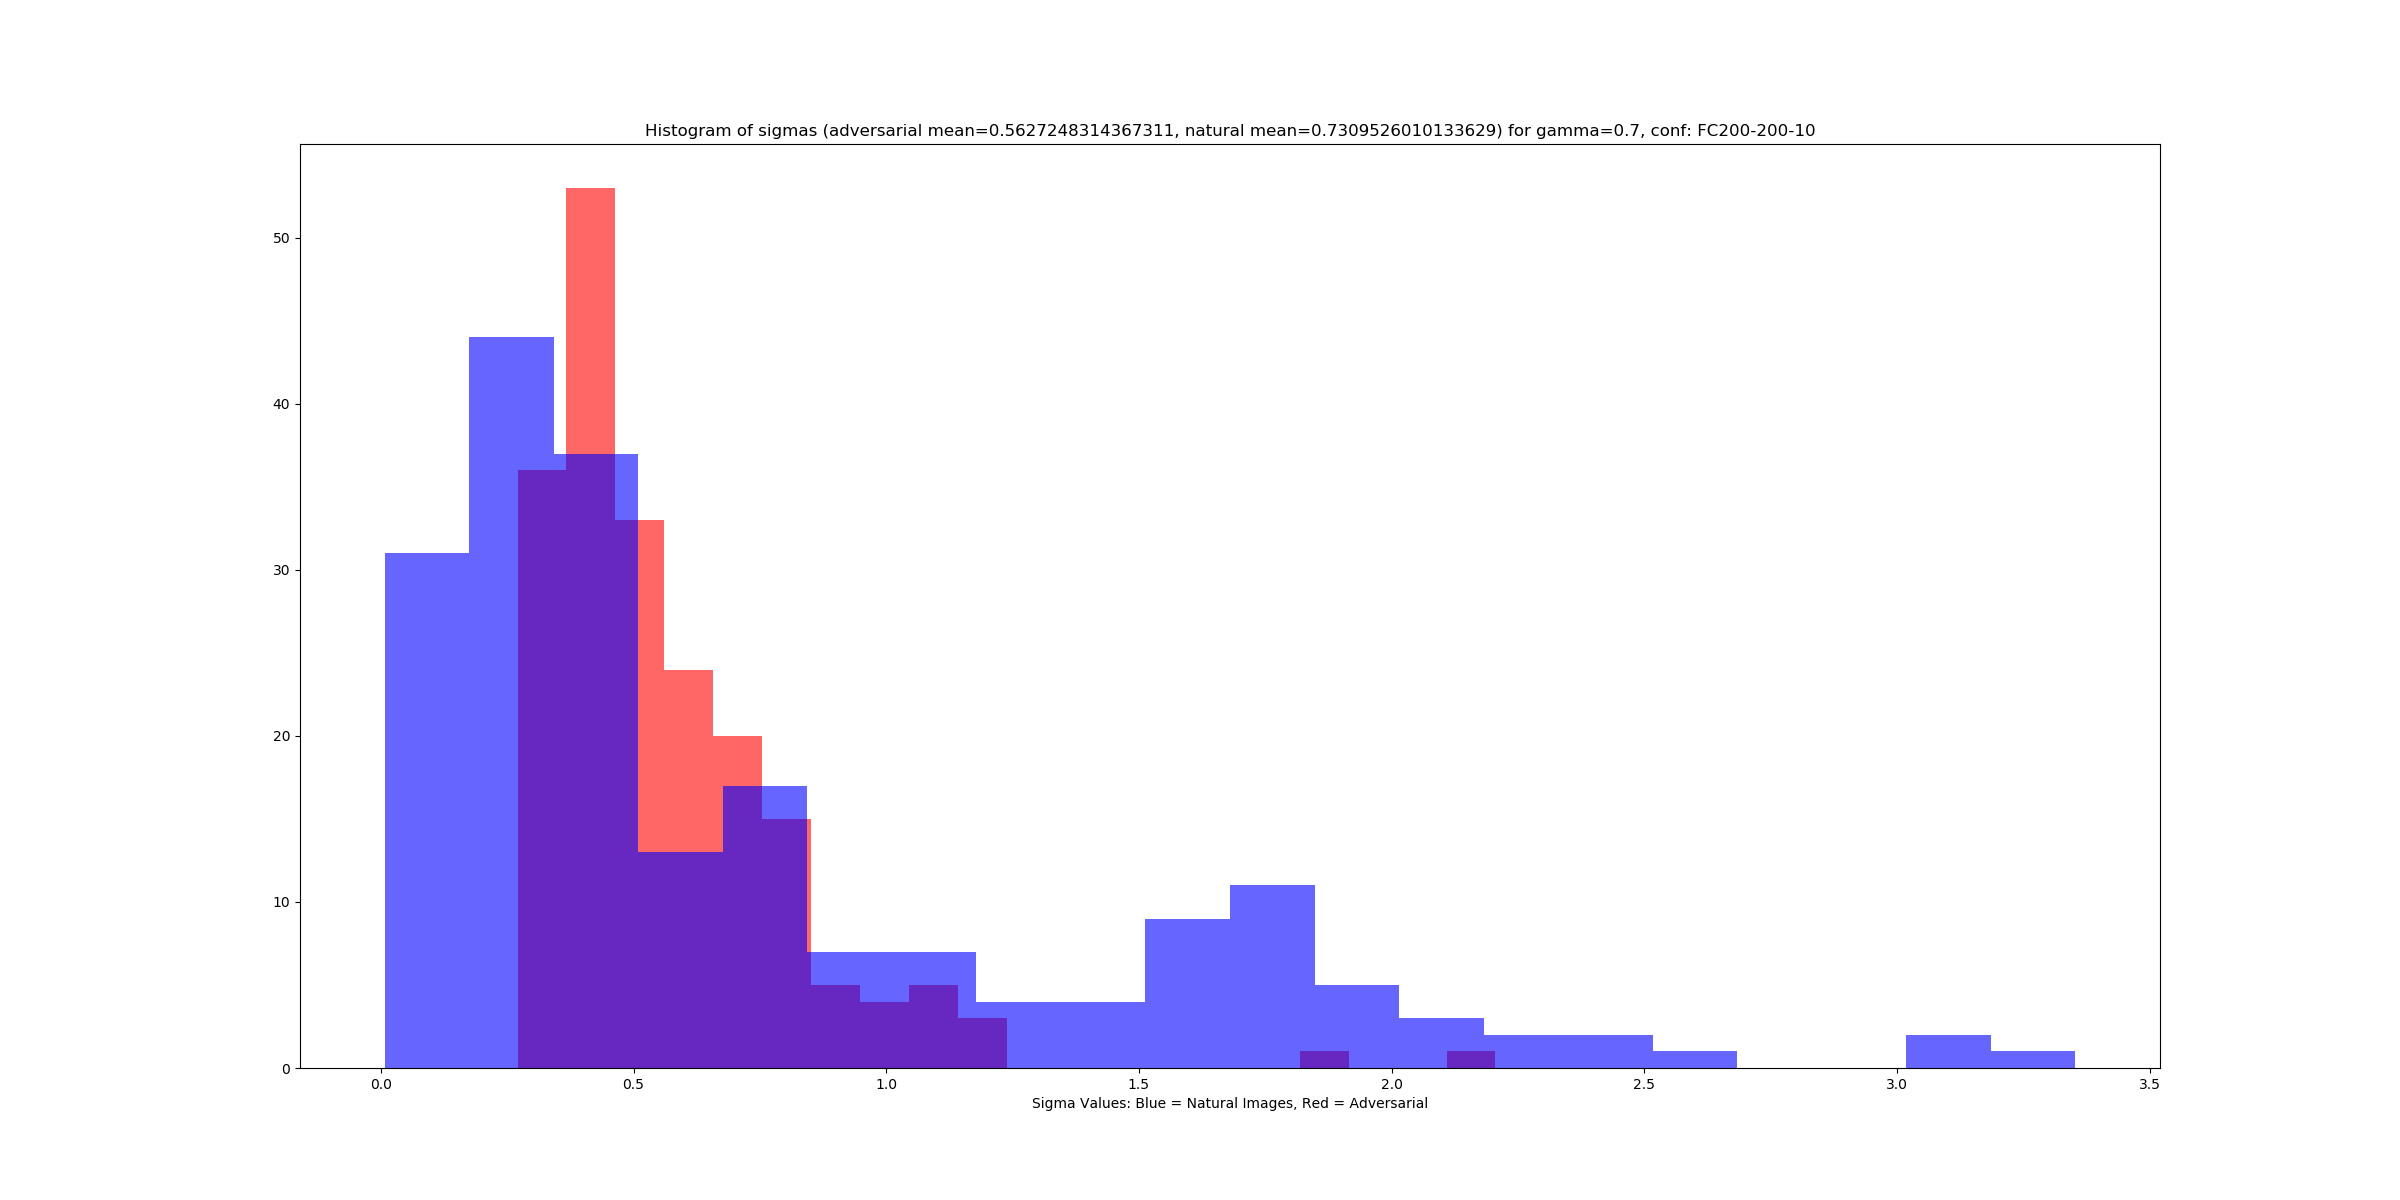
\includegraphics[trim=200 80 100 100, clip,width=7cm]{c2_figures/FC200-200-10-gamma1_hist.png}
% \caption{Distortion (left) and $0.7$-persistence (right) for FC200-200-10 in Table \ref{table1}}
% \label{table1hist5}
% \end{figure}

%\subsection{CNNs work}

% \section{Conclusion}
% In general, our intuition that adversarial examples are less stable than than natural examples is supported by the results in Table \ref{table1}. 

% The more complex neural networks tended to support less stable adversarial examples, but ones that are closer to the natural examples. 

% Need better discussion and conclusion.
% Key takeaways: 
% 1) Perturbations of adversarial examples do not tend to regress to the original class, but rather to some central class. (Is this still true for Imagenet?)

% Similar to the suggestions of ~\cite{Fawzi2018empirical}, our methods have exploited a notion of curvature based on measures with expanding concentration. A typical example of this method is the tube formulas in integral geometry based on Steiner's early work and greatly generalized to the cases of manifolds, polyhedra, and sets of positive reach \cite{morvan}. These are based on taking uniform measures on balls around the spaces. While this notion is generally considered by taking balls around entire sets, the ideas can also be used to investigate individual points. We consider Gaussian sampling instead because of its ease of use, but the idea that we can change the standard deviations is analogous to changing the radius of uniformly sampled balls. Moreover, concentration inequalities indicate that in high dimensions both cases result in concentration of measure around balls of a radius related to either the standard deviation or radius, respectively (see Section \ref{sec:concentration}). In fact, it may be the case that the differences in the estimates in Proposition \ref{prop:concentration} indicate that Gaussian sampling is, in fact, better than uniform sampling of the ball since the concentration in annuli does not depend on the standard deviation in the case of Gaussian and does depend on radius in the case of uniform.



%, Gaussian measures try to exploit similar structure, but is done in a different way by doing Gaussian sampling about a point instead of approximating curvatures of decision boundaries. Since the results in \cite{Fawzi2018empirical} are based on computing an approximation of a curvature function, they depend on an assumption of being close to the decision boundary. Our method does not need that assumption since the Gaussian sampling is not related to functions but instead based on measures. Curvatures have a close connection to tube formulas \cite{morvan}, which is related to the uniform measure on balls. These measures may not be well-behaved in high dimensions, which is one of the main reasons we choose to instead consider Gaussian measures, which factorize nicely in high dimensions.
%\todo{[DG]: These need to be expanded and placed here or elsewhere, but are extremely important.}



% In these results, we first notice that adversarial attacks generated with IGSM against MNIST are less stable than natural examples from these data sets. This difference is even more pronounced when comparing a adversarial image with other image samples from its target class. This lower stability of adversarial examples is even more pronounced among the attacks prepared via IGSM against VGG16 on ImageNet. Using this technique, we can distinguish adversarial examples prepared by these techniques from natural examples using stability as a test. 

% In the next section of experiments, Table 1 from \cite{Szegedy2013} was reconstructed and augmented with stability measurements. In this table, of the 5 networks trained on the MNIST dataset, the more complicated networks achieved higher accuracy but were defeated by adversarial examples with much less distortion than the simpler adversarial examples. We have added columns indicating the stability of natural and adversarial examples in these models. Adversarial examples generated for more complicated models were much less stable (some less stable than the corresponding natural examples). Adversarial examples generated for the less complicated networks were vastly more stable than natural examples. These results are summarized in the histograms Figure \ref{table1hist1} through \ref{table1hist5}. 

% Type 1: An image whose object measure does not exist under a random
% process $F_w$. This may be recognized in the image space if the
% manifold of measures is observed in the image space. This manifold
% should be of relatively low dimension compared with the dimension of
% the image space, and any images thatvary in directions orthogonal to
% the manifold satisfy Type 1.\\

% \vspace{.3cm}

% e.g. We can consider the image of the
% set of possible handwritten digits under a noiseless
% discretization $A$. It is assumed that the image of the manifold $M$ of
% handwritten digits in $X_O$, $A(M)$ is low dimensional in $X_I$, thus we can 

% \vspace{.3cm}

% consider an $\e$-triangulation of this manifold under $A$ with $\e$
% the resolution of $A$. A type 1 adversarial image will
% be identified as any image that varies more than $\e$ from the
% simplices connecting the triangulation of $A(M)$. 

% Type 2: A perturbation of an image that is indistinguishable under the
% imaging operation (or stochastic imaging process) from an image of an
% admissible object.

%%%%%%%%%%%%%%%%%%%%%%%%%%%%%%%%%%%%%%%%%%%(2)

% \section{Conclusion/Ongoing Work (incorporate in previous)}
% Through the work of Szegedy et al, it was discovered that more sophisticated DNNs can be fooled with smaller adversarial perturbations than less sophisticated DNNs. This speaks to a trade-off between robustness and accuracy which has continued to be an active area of research \cite{tsipras2018robustness}. In this work, we investigated this further by examining neighborhoods around adversarial and natural examples using sampling and $(\gamma,\sigma)$ stability analysis. The same trade-off was observed and we note that highly sophisticated networks admit adversarial examples with very small distortion which can often be identified by a sampling technique. We conclude that such subtle adversarial examples are often not $(\gamma,\sigma)$ stable. One direction for future work is the combination of this sampling method for analyzing neighborhoods with recent geometric interpretations of neural networks. It is theorized that most imaging datasets are samples of low-dimensional manifolds embedded in much higher dimensional representation spaces \cite{Chang2017}. By sampling neighborhoods, we can identify these manifolds and potentially train neural networks which are better restricted to them.  

% Continuing research will focus on understanding the trade-off between the sophistication (corresponding with accuracy) and the distortion and stability of adversarial examples that can be generated. Further numerical experiments can be focused on exploring the geometric properties of trained DNNs. We have observed in this report that the average distortion of examples which achieve a new adversarial class vary non-linearly among different natural images and different network structures. Investigating $(\gamma,\sigma)$ stability of points on paths between natural and adversarial examples or between different natural images may provide more insight into the geometric interpretation of classification boundaries under DNN models. In addition, there are many more adversarial attack types that can be subjected to this analysis.  We have seen that some robust networks only admit adversarial examples with very significant distortion, while other networks admit examples with much smaller distortion. In particular, there is the outstanding question of extending a definition for adversarial examples which emphasizes the subtlety of such examples. 

% Some recent work on this subject has distinguished "fooling" examples which are images that look nothing like the training \cite{nguyen2015deep}. In their work, Nguyen et al. were able to reliably identify such examples through the use of Generative Adversarial Network discriminators. One interesting experiment would be to test GAN discriminators on adversarial examples with varying distortion. If GANs can distinguish adversarial examples with high distortion, while examples with low distortion are less $(\gamma,\sigma)$ stable than natural images, this may establish a no-free-lunch classification of Adversarial Examples. Such classification would have broad implications across the field of machine-learning. 



%Kevin Lin, Mingwei
%Grant funding: BB/DG/KH/CS NSF CCF 1740858 
%Grant funding: BB/DG: NSF DMS 1937229
%Grant funding: DG: NSF DMS 1760538

